 %%%%%%%%%%%%%%%%%%%%%%%%%%%%%%%%%%%%%%%%%%%%%%%%%%%%%%%%%%%%%%%%%%%%%%
% How to use writeLaTeX: 
%
% You edit the source code here on the left, and the preview on the
% right shows you the result within a few seconds.
%
% Bookmark this page and share the URL with your co-authors. They can
% edit at the same time!
%
% You can upload figures, bibliographies, custom classes and
% styles using the files menu.
%
% If you're new to LaTeX, the wikibook is a great place to start:
% http://en.wikibooks.org/wiki/LaTeX
%
%%%%%%%%%%%%%%%%%%%%%%%%%%%%%%%%%%%%%%%%%%%%%%%%%%%%%%%%%%%%%%%%%%%%%%
\documentclass[]{tufte-book}
%\hypersetup{colorlinks}% uncomment this line if you prefer colored hyperlinks (e.g., for onscreen viewing)
\usepackage[frenchb]{babel}
\usepackage[utf8]{inputenc}
%%
% Book metadata
\title{Cosmologie Physique}
%\subtitle{Cosmologie Physique}
\author[Dominique Aubert]{Dominique Aubert}
\publisher{Ellipses}

%%
% If they're installed, use Bergamo and Chantilly from www.fontsite.com.
% They're clones of Bembo and Gill Sans, respectively.
%\IfFileExists{bergamo.sty}{\usepackage[osf]{bergamo}}{}% Bembo
%\IfFileExists{chantill.sty}{\usepackage{chantill}}{}% Gill Sans

%\usepackage{microtype}

%%


% Just some sample text
\usepackage{lipsum}

%%
% For nicely typeset tabular material
\usepackage{booktabs}

%%
% For graphics / images
\usepackage{graphicx}
\setkeys{Gin}{width=\linewidth,totalheight=\textheight,keepaspectratio}
\graphicspath{{graphics/}}

% The fancyvrb package lets us customize the formatting of verbatim
% environments.  We use a slightly smaller font.
\usepackage{fancyvrb}
\fvset{fontsize=\normalsize}

%%
% Prints argument within hanging parentheses (i.e., parentheses that take
% up no horizontal space).  Useful in tabular environments.
\newcommand{\hangp}[1]{\makebox[0pt][r]{(}#1\makebox[0pt][l]{)}}

%%
% Prints an asterisk that takes up no horizontal space.
% Useful in tabular environments.
\newcommand{\hangstar}{\makebox[0pt][l]{*}}

%%
% Prints a trailing space in a smart way.
\usepackage{xspace}

%%
% Some shortcuts for Tufte's book titles.  The lowercase commands will
% produce the initials of the book title in italics.  The all-caps commands
% will print out the full title of the book in italics.
\newcommand{\vdqi}{\textit{VDQI}\xspace}
\newcommand{\ei}{\textit{EI}\xspace}
\newcommand{\ve}{\textit{VE}\xspace}
\newcommand{\be}{\textit{BE}\xspace}
\newcommand{\VDQI}{\textit{The Visual Display of Quantitative Information}\xspace}
\newcommand{\EI}{\textit{Envisioning Information}\xspace}
\newcommand{\VE}{\textit{Visual Explanations}\xspace}
\newcommand{\BE}{\textit{Beautiful Evidence}\xspace}

\newcommand{\TL}{Tufte-\LaTeX\xspace}

% Prints the month name (e.g., January) and the year (e.g., 2008)
\newcommand{\monthyear}{%
  \ifcase\month\or January\or February\or March\or April\or May\or June\or
  July\or August\or September\or October\or November\or
  December\fi\space\number\year
}


% Prints an epigraph and speaker in sans serif, all-caps type.
\newcommand{\openepigraph}[2]{%
  %\sffamily\fontsize{14}{16}\selectfont
  \begin{fullwidth}
  \sffamily\large
  \begin{doublespace}
  \noindent\allcaps{#1}\\% epigraph
  \noindent\allcaps{#2}% author
  \end{doublespace}
  \end{fullwidth}
}

% Inserts a blank page
\newcommand{\blankpage}{\newpage\hbox{}\thispagestyle{empty}\newpage}

\usepackage{units}

% Typesets the font size, leading, and measure in the form of 10/12x26 pc.
\newcommand{\measure}[3]{#1/#2$\times$\unit[#3]{pc}}

% Macros for typesetting the documentation
\newcommand{\hlred}[1]{\textcolor{Maroon}{#1}}% prints in red
\newcommand{\hangleft}[1]{\makebox[0pt][r]{#1}}
\newcommand{\hairsp}{\hspace{1pt}}% hair space
\newcommand{\hquad}{\hskip0.5em\relax}% half quad space
\newcommand{\TODO}{\textcolor{red}{\bf TODO!}\xspace}
\newcommand{\ie}{\textit{i.\hairsp{}e.}\xspace}
\newcommand{\eg}{\textit{e.\hairsp{}g.}\xspace}
\newcommand{\na}{\quad--}% used in tables for N/A cells
\providecommand{\XeLaTeX}{X\lower.5ex\hbox{\kern-0.15em\reflectbox{E}}\kern-0.1em\LaTeX}
\newcommand{\tXeLaTeX}{\XeLaTeX\index{XeLaTeX@\protect\XeLaTeX}}
% \index{\texttt{\textbackslash xyz}@\hangleft{\texttt{\textbackslash}}\texttt{xyz}}
\newcommand{\tuftebs}{\symbol{'134}}% a backslash in tt type in OT1/T1
\newcommand{\doccmdnoindex}[2][]{\texttt{\tuftebs#2}}% command name -- adds backslash automatically (and doesn't add cmd to the index)
\newcommand{\doccmddef}[2][]{%
  \hlred{\texttt{\tuftebs#2}}\label{cmd:#2}%
  \ifthenelse{\isempty{#1}}%
    {% add the command to the index
      \index{#2 command@\protect\hangleft{\texttt{\tuftebs}}\texttt{#2}}% command name
    }%
    {% add the command and package to the index
      \index{#2 command@\protect\hangleft{\texttt{\tuftebs}}\texttt{#2} (\texttt{#1} package)}% command name
      \index{#1 package@\texttt{#1} package}\index{packages!#1@\texttt{#1}}% package name
    }%
}% command name -- adds backslash automatically
\newcommand{\doccmd}[2][]{%
  \texttt{\tuftebs#2}%
  \ifthenelse{\isempty{#1}}%
    {% add the command to the index
      \index{#2 command@\protect\hangleft{\texttt{\tuftebs}}\texttt{#2}}% command name
    }%
    {% add the command and package to the index
      \index{#2 command@\protect\hangleft{\texttt{\tuftebs}}\texttt{#2} (\texttt{#1} package)}% command name
      \index{#1 package@\texttt{#1} package}\index{packages!#1@\texttt{#1}}% package name
    }%
}% command name -- adds backslash automatically
\newcommand{\docopt}[1]{\ensuremath{\langle}\textrm{\textit{#1}}\ensuremath{\rangle}}% optional command argument
\newcommand{\docarg}[1]{\textrm{\textit{#1}}}% (required) command argument
\newenvironment{docspec}{\begin{quotation}\ttfamily\parskip0pt\parindent0pt\ignorespaces}{\end{quotation}}% command specification environment
\newcommand{\docenv}[1]{\texttt{#1}\index{#1 environment@\texttt{#1} environment}\index{environments!#1@\texttt{#1}}}% environment name
\newcommand{\docenvdef}[1]{\hlred{\texttt{#1}}\label{env:#1}\index{#1 environment@\texttt{#1} environment}\index{environments!#1@\texttt{#1}}}% environment name
\newcommand{\docpkg}[1]{\texttt{#1}\index{#1 package@\texttt{#1} package}\index{packages!#1@\texttt{#1}}}% package name
\newcommand{\doccls}[1]{\texttt{#1}}% document class name
\newcommand{\docclsopt}[1]{\texttt{#1}\index{#1 class option@\texttt{#1} class option}\index{class options!#1@\texttt{#1}}}% document class option name
\newcommand{\docclsoptdef}[1]{\hlred{\texttt{#1}}\label{clsopt:#1}\index{#1 class option@\texttt{#1} class option}\index{class options!#1@\texttt{#1}}}% document class option name defined
\newcommand{\docmsg}[2]{\bigskip\begin{fullwidth}\noindent\ttfamily#1\end{fullwidth}\medskip\par\noindent#2}
\newcommand{\docfilehook}[2]{\texttt{#1}\index{file hooks!#2}\index{#1@\texttt{#1}}}
\newcommand{\doccounter}[1]{\texttt{#1}\index{#1 counter@\texttt{#1} counter}}

%\newcommand{\newthought}[1]{{#1}} 
%\newcommand{\newthought}[1]{{#1}}
% Generates the index
\usepackage{makeidx}
%\usepackage[toc]{glossaries}
\makeindex
%\makeglossaries

\begin{document}

% Front matter
\frontmatter

% r.1 blank page
\blankpage

% v.2 epigraphs
\newpage\thispagestyle{empty}
\openepigraph{%
Manuscrit entamé le 29 Juin 2017 à l'observatoire astronomique de Strasbourg.
}{Paul Rand%, {\itshape Design, Form, and Chaos}
}
%\vfill
%\openepigraph{%
%A designer knows that he has achieved perfection 
%not when there is nothing left to add, 
%but when there is nothing left to take away.
%}{Antoine de Saint-Exup\'{e}ry}
%\vfill
%\openepigraph{%
%\ldots the designer of a new system must not only be the implementor and the first 
%large-scale user; the designer should also write the first user manual\ldots 
%If I had not participated fully in all these activities, 
%literally hundreds of improvements would never have been made, 
%because I would never have thought of them or perceived 
%why they were important.
%}{Donald E. Knuth}


% r.3 full title page
\maketitle


% v.4 copyright page
%\newpage
%\begin{fullwidth}
%~\vfill
%\thispagestyle{empty}
%\setlength{\parindent}{0pt}
%\setlength{\parskip}{\baselineskip}
%Copyright \copyright\ \the\year\ \thanklessauthor
%
%\par\smallcaps{Published by \thanklesspublisher}
%
%\par\smallcaps{tufte-latex.googlecode.com}
%
%%\par Licensed under the Apache License, Version 2.0 (the ``License''); you may not
%use this file except in compliance with the License. You may obtain a copy
%of the License at \url{http://www.apache.org/licenses/LICENSE-2.0}. Unless
%required by applicable law or agreed to in writing, software distributed
%under the License is distributed on an \smallcaps{``AS IS'' BASIS, WITHOUT
%WARRANTIES OR CONDITIONS OF ANY KIND}, either express or implied. See the
%License for the specific language governing permissions and limitations
%under the License.\index{license}

%\par\textit{First printing, \monthyear}
%\end{fullwidth}

% r.5 contents
\tableofcontents
%\listoffigures

% \listoftables

%% r.7 dedication
%\cleardoublepage
%~\vfill
%\begin{doublespace}
%\noindent\fontsize{18}{22}\selectfont\itshape
%\nohyphenation
%Dedicated to those who appreciate \LaTeX{} 
%and the work of \mbox{Edward R.~Tufte} 
%and \mbox{Donald E.~Knuth}.
%\end{doublespace}
%\vfill
%\vfill


% r.9 introduction
\cleardoublepage

\include{Intro}

%%
% Start the main matter (normal chapters)
\mainmatter

%%!TEX root = /Users/domaubert/Documents/Lectures/cosmologie/cosmo_main.tex
\chapter{Etat des connaissances}

%\textit{Ce chapitre est tiré de \textbf{The Cosmological Parameters}, Lahav et Liddle, arxiv1401.1389}
%\newline
%\newline

L'objectif de ce chapitre est de faire un court panorama de l'état de nos connaissances sur les propriétés observées de l'Univers. Les chapitres suivant seront eux consacrés à l'élaboration des concepts et des théories qui permettent de rendre compte de ces propriétés observées. 

Concernant notre connaissance des propriétés de l'Univers, elle repose souvent sur \textit{l'interprétation d'observations au travers de théories et de modèles}. Par conséquent les propriétés décrites dans ce chapitre sont essentiellement valable dans le contexte du modèle standard de la cosmologie décrit dans les chapitres suivants. Si un changement de paradigme vient à opérer, rien n'empêche à priori que ces observations soit réinterprétées et donc conduise à modifier ce que nous savons de l'Univers.

\section{Observation fondamentale : le décalage vers le rouge}
L'observation première de la cosmologie, à l'origine même de l'émergence de la discipline au début du 20ème siècle, est la constatation que tous les objets observés à grande distance sont plus "rouges" qu'attendus. La mesure du spectre de ces objets indiquent que les systèmes de raies observés, parfois complexes, sont tous à des longueurs d'ondes plus importantes que ce que l'observation de ces mêmes éléments aurait donné dans un laboratoire. On définit le décalage vers le rouge ou "redshift" par la quantité z\index{redshift}
\begin{equation}
z\equiv\frac{\lambda-\lambda_0}{\lambda_0},
\end{equation}
où $\lambda$ est la longueur d'onde\index{longueur d'onde} observée et $\lambda_0$ celle mesurée en laboratoire. De plus ce rougissement est d'autant plus grand que la source est éloignée. 

Dans le cadre du modèle standard de la cosmologie, ce rougissement est de nature \textit{cosmologique} et traduit le phénomène \textit{d'expansion} de l'Univers. Dans ce processus d'expansion, toute distance prise entre 2 points de l'Univers est amené à évoluer \sidenote{en l'occurrence à augmenter dans un modèle standard d'Univers}. Notons dès à présent que cette augmentation n'est pas le symptôme d'un déplacement des sources par rapport à leur espace local mais plutôt la conséquence d'une dilatation de l'espace entre l'observateur et la source. Cette dilatation agit également sur la longueur d'onde des photons en vol et conduit au rougissement observé. Cette dilatation agit aussi sur les densités, diluant au cours du temps de telles quantités et on peut montrer qu'elle produit des dilatations des durées, on allongeant tout types d'intervalles temporels. Enfin, cette interprétation cosmologique permet également d'expliquer pourquoi ce décalage vers le rouge est d'autant plus important que la source est éloignée.

Notons que comme le redshift croît avec la distance, $z$ est de façon indirecte un indicateur de \textit{distance} et comme la lumière nous parvient avec une vitesse finie et connue, $z$ est également un indicateur de \textit{l'époque} à laquelle la source est observée. En cosmologie, l'action de désigner un objet ou un phénomène par son redshift $z$ implique à la fois une information spectrale, spatiale et temporelle.

Le processus d'expansion a débuté il y a 13.8 milliards d'années: c'est le \textit{Big Bang}\index{Big Bang}. Aux premiers instants, les distances étaient présumément courtes, l'Univers était donc de fait très dense. Régnait également une température très élevée, qui fut amenée à décroître au cours du temps\sidenote{Par exemple la température du 'gaz de photons cosmique', le fond diffus cosmologique, est aujourd'hui de 2.73 K mais était environ 1000 fois plus chaud lorsqu'il a été libéré. }. De fait le modèle accepté permettant de décrire les origines de l'Univers est parfois dénommé modèle du \textit{Big Bang chaud}.

\section{Propriétés générales de l'Univers}
L'Univers dans lequel nous vivons peut, semble-t-il, être décrit par une poignée de paramètres. La connaissance de ceux-ci, ajoutée à la connaissance de ce que nous croyons être les bonnes lois de la physique, permet d'expliquer une très grande partie des propriétés globales de l'Univers et également une grande partie des processus astrophysiques qui subissent la cosmologie qui les entoure.  

\subsection{Paramètres cosmologiques}
Comme détaillé dans les chapitres suivant, l'Univers peut être décrit à un haut niveau de précision en considérant qu'il est homogène, isotrope et possédant une dynamique régie par les équations de la relativité générale. Toutefois cette description nécessite la connaissance à priori de certains paramètres qui permettent d'expliquer l'Univers tel qu'il est observé. A l'inverse l'observation de l'état actuel du cosmos met des contraintes sur la valeur de ces paramètres.

\paragraph{Paramètre de Hubble} Le premier paramètre est le paramètre de Hubble $H_0$ \index{Hubble!paramètre}, qui caractérise le taux d'expansion actuel. Sa valeur est d'environ 70 km/s/Mpc. On utilise parfois le paramètre de Hubble réduit $h$ tel que $H_0=100 h$ km/s/Mpc~: sa valeur est proche $h\sim 0.7$.

\paragraph{Paramètres de densité} Les différents types d'énergie présents dans l'Univers ont une grande influence sur ses propriétés et leurs contribution au budget énergétique total est caractérisé par des paramètres de densité $\Omega_i$ \index{paramètre ! densité}. En pratique c'est le rapport de la densité d'énergie de type $i$ à une densité d'énergie de référence appelée \textit{densité critique\index{densité critique}}. On distingue la densité de matière $\Omega_m$, la densité de baryons (protons+neutrons(+électrons)) $\Omega_b$, la densité de rayonnement $\Omega_r$, la densité d'énergie des neutrinos $\Omega_\nu$ et la densité d'énergie noire\index{energie noire @énergie noire} $\Omega_\Lambda$. Il faut noter que la contribution de la matière contient celle des baryons\index{baryons}, par conséquent $\Omega_m\ge\Omega_b$: actuellement on a $\Omega_m\sim 0.3$ et $\Omega_b\sim 0.05$, la différence étant la contribution apportée par une matière \textit{non baryonique}, dite matière noire\index{matière noire}. Les contributions des espèces relativistes (photons, neutrinos) est aujourd'hui négligeable, bien que ce type de particule soit très abondant en nombre.

\paragraph{Spectre de fluctuations initiales} L'Univers tel qu'observé actuellement n'est pas strictement homogène, en particulier sur des échelles inférieures à la dizaine de Mpc. Les galaxies et amas qui nous entourent trouvent leur origine dans des fluctuations\index{fluctuations de densité} initiales de densité de très faible amplitude. Ces fluctuations sont caractérisées par un spectre  $P(k)$ qui donne la distribution des amplitudes des fluctuations de taille $L=2\pi/k$. On suppose actuellement que celles-ci trouvent leur origine dans la période \textit{d'inflation} qui prédit un spectre primordial de la forme \index{spectre ! puissance} :
\begin{equation}
P(k)\sim  k^{n_s},
\end{equation} 
$n_s$ constitue également un paramètre cosmologique et les modèles inflationnaire lui prédise une valeur \textit{proche mais différente} de \index{spectre ! inflation} l'unité \sidenote{le satellite Planck mesure ainsi une valeur proche de 0.96}. L'amplitude globale du spectre doit également être paramétrée, par exemple sous la forme d'une amplitude de fluctuation sur une échelle arbitraire de 8 Mpc, notée $\sigma_8$\index{spectre ! amplitude}. Notons enfin que les modèles d'inflations prédisent un fond d'ondes gravitationnelles\index{ondes gravitationnelles}, caractérisé par un spectre de fluctuations tensorielles, similaire à celui des fluctuations de densité (dites également scalaires). Le rapport d'amplitude entre fluctuations tensorielles et scalaires est noté $r$ et sa valeur est supposée quasi-nulle.

\paragraph{Etat d'ionisation de l'Univers} Le dernier paramètre canonique de la cosmologie permet de décrire l'état d'ionisation \index{ionisation} de l'Univers au cours de son histoire. Cet état se mesure en  contraignant le nombre moyen de diffusions des photons\index{photons} sur les électrons libres du cosmos\index{electrons@électrons}. Cette quantité est notée $\tau$ avec une valeur typique $\tau \sim 0.07$. L'essentiel de ces électrons libres sont produits au cours de la réionisation de l'Univers au redshift $z_\mathrm{reion}\sim 8$: dans les modèles les plus simples $\tau$ et $z_\mathrm{reion}$ sont directement liés.

\paragraph{Modèle minimal} L'ensemble des paramètres décrit précédemment permettent de rendre compte d'une grande variétés de propriétés observables. D'autre part, certaines hypothèses permettent encore de réduire le nombre de paramètres libres. Par exemple, l'inflation prédit une courbure\index{courbure} intrinsèque nulle qui se traduit en pratique par $\sum_i \Omega_i=1$. D'autre part l'amplitude des modes tensoriels (i.e. les ondes gravitationnelles issues de l'inflation) étant attendue comme très faible, on peut aisément poser $r=0$. Enfin, le paramètre de densité de rayonnement $\Omega_r$ est très précisément mesuré, par la mesure de température précise du fond diffus\index{fond diffus} ($T=2.7255\pm0.0006$ K) et ne permet donc plus de latitude significative sur sa valeur. Enfin , en l'absence de physique exotique la densité d'énergie des neutrinos $\Omega_\nu$ est directement liée à celle des photons \sidenote{tout en étant quasi nulle aujourd'hui}. Au final, un modèle extrêmement solide peut être construit avec seulement 6 paramètres libres. Au choix typique de "sextet" est $(\Omega_b,\Omega_m, H_0,\sigma_8,n_s,\tau)$. Bien sûr d'autres combinaisons de paramètres libres sont possibles.

\subsection{Principales sondes observationnelles}

Les paramètres précédents sont contraints par l'observation croisée de différentes sondes observationnelle. La convergence de ces valeurs conduit à ce qui est communément nommé \textit{le modèle de concordance}. Voici une liste (non-exhaustive) des principales sondes cosmologiques.

\paragraph{Mesure directe de $H_0$}
Cette mesure s'effectue à l'aide de chandelles standards qui permettent de mesurer indépendamment la distance d'un objet extra-galactique et son redshift $z$. La chandelle de référence est la relation période luminosité des étoiles variables de type Céphéides\index{Céphéides} la mesure de la période permet de déterminer la luminosité intrinsèque et donc la distance. Les Céphéides sont des indicateurs primaires et permettent de calibrer des indicateurs secondaires: courbes de lumières des supernovæ, relation de Tully-Fisher, etc... Ce type d'indicateurs donne une valeur de $H_0\sim 73$ km/s/Mpc. Le fond diffus cosmologique permet également une mesure indépendante de $H_0\sim 67$ km/s/Mpc en légère tension avec les estimateurs précédents.

\paragraph{Supernovæ et cosmologie}
La grande luminosité des supernovæ permet leur détection à des distances cosmologiques. De plus certains types de supernovæ\index{supernovae}, celles dite de type 'SN1A', ont un caractère quasi standard car elles résultent de l'explosion de naine blanche dans des systèmes binaires pour lesquelles il existe une forte corrélation entre luminosité et paramètres de la courbe de luminosité. L'accélération\index{accélération} \sidenote{c'est-à-dire le fait que les distances augmentent de plus en plus rapidement aujourd'hui} de l'expansion de l'Univers a été mise en évidence pour la première fois à l'aide de ce type d'indicateurs, en proposant pour la première fois la combinaison $\Omega_m=0.3$ et $\Omega_\Lambda=0.7$. De plus ces mêmes indicateurs indiquent que la densité d'énergie noire\index{energie noire@énergie noire} est une constante, donc équivalente à une constante cosmologique\index{constante cosmologique}\sidenote{on rencontrera aussi parfois le terme d'énergie du vide}.

\paragraph{Le fond diffus cosmologique}
Le fond diffus\index{fond diffus} cosmologique (Cosmic Microwave Background, CMB) est constitué des photons produits lors de la recombinaison\index{recombinaison}, 380 000 ans après le Big-Bang. Il constitue le plus grand réservoir de photons du cosmos et présente une brillance homogène à des niveaux de 1 pour 100 000. Le CMB présente néanmoins de faibles inhomogénéités qui tracent les inhomogénéités de matière à cette époque. La structure spatiale (en fait angulaire sur le ciel) comprend des informations sur toute l'histoire de croissance des structures depuis le Big-Bang jusqu'à 380 000 ans plus tard et sur les processus de couplage entre le rayonnement et la matière. L'étude de ces fluctuations permet par exemple d'établir la platitude de la géométrie de l'Univers, fournit une mesure de la quantité de baryons $\Omega_b$\index{baryons}, confirme la nécessité d'une matière non-baryonique et l'absence d'évolution de l'énergie noire. Le CMB indique également que le spectre de fluctuation initial est consistant avec les modèles d'inflation \index{inflation} et pour l'instant les modes tensoriels restent indétectables. Enfin le nombre de diffusion \index{diffusion} des photons sur les électrons est de l'ordre de $\tau\sim 0.07$ correspondant à une réionization vers un redshift de $z\sim8$. Le CMB constitue à l'heure actuelle la sonde la plus précise et la plus complète d'informations cosmologiques. C'est l'objet d'étude de missions spatiales et sol de très grande ampleur, dont par exemple le satellite européen \textit{Planck}.

\begin{figure}[htbp]
	\centering
		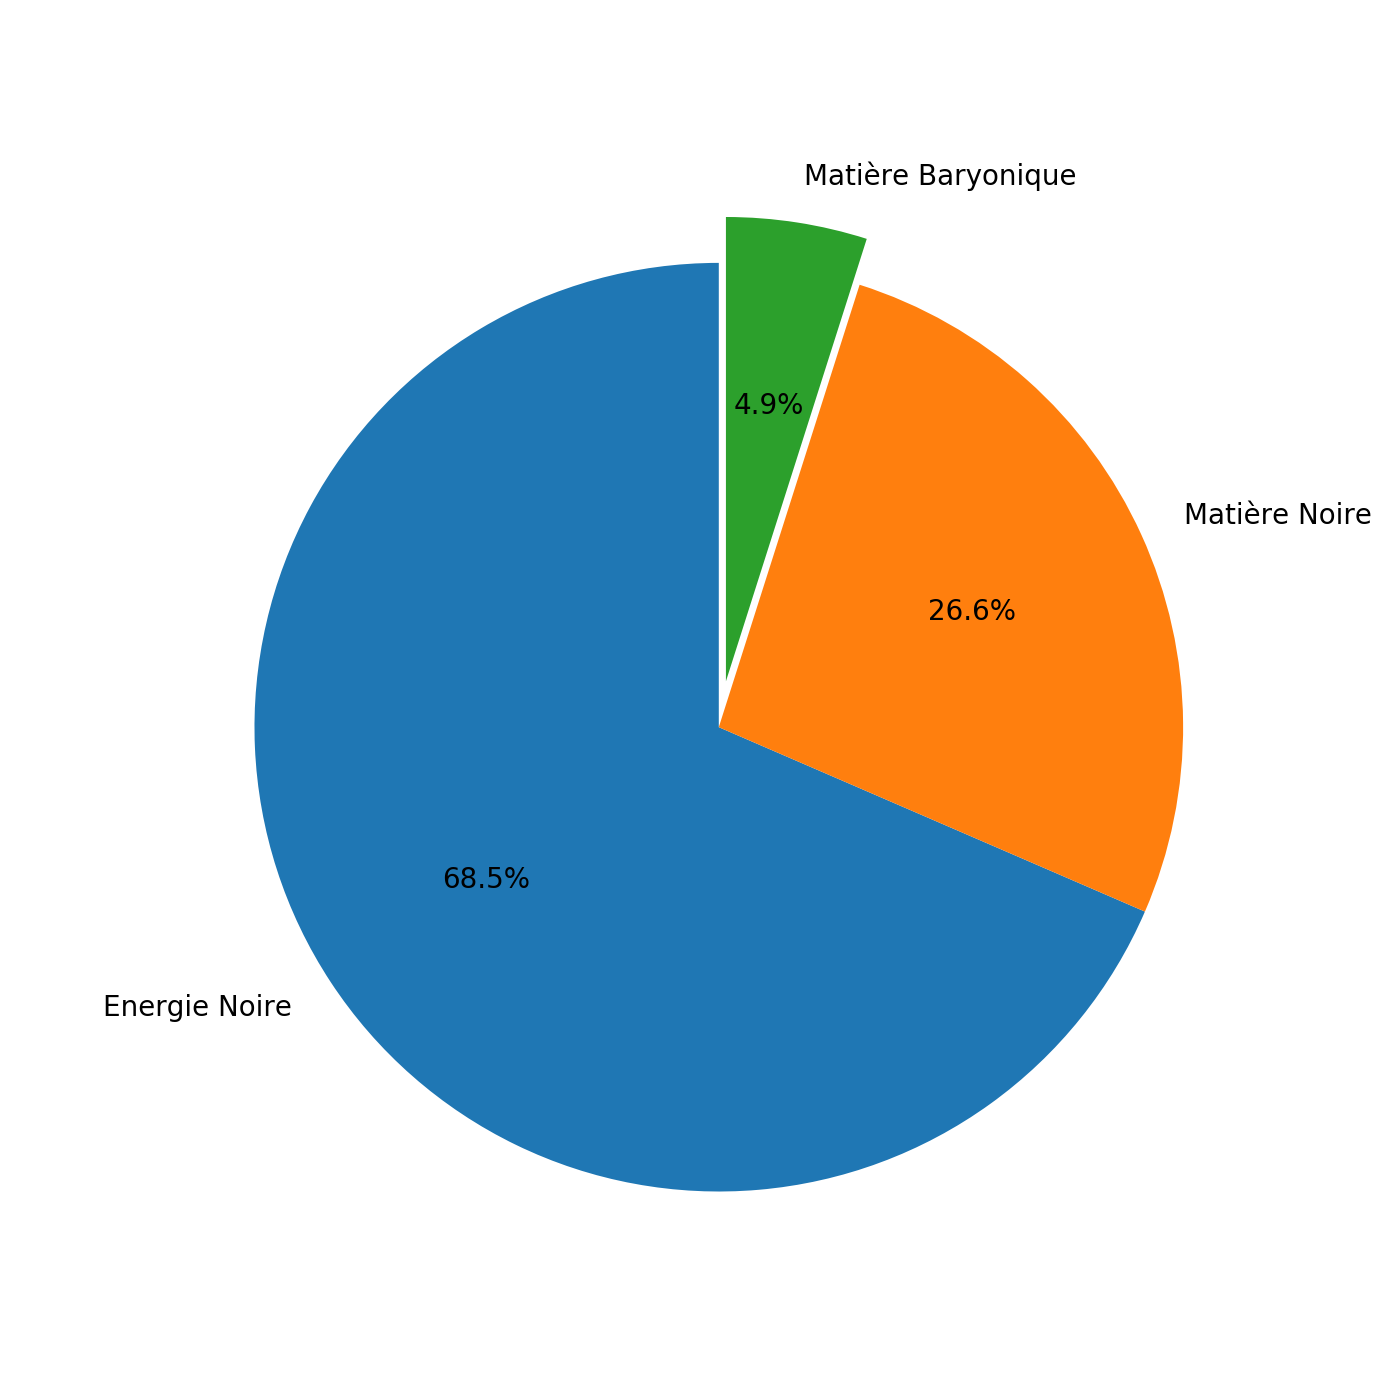
\includegraphics[height=10cm]{figs/pieplanck.png}
		\caption[Le bilan énergétique de l'Univers]{La répartition des différentes formes d'énergie au bilan énergétique total de l'Univers, d'après les mesures du satellite \textit{Planck}. On note l'absence de contribution du rayonnement et des neutrinos, dont le poids énergétique est trop faible pour pouvoir être représenté ici. La matière 'normale', désignée comme 'baryonique' et composée de protons, neutrons et électrons ne représente que $\sim 5\%$ du total. Le reste constitue le \textit{secteur sombre}.}
	\label{f:timeline}
\end{figure}


\paragraph{Grands relevés de Galaxies}
Les galaxies \index{galaxies} constituent des traceurs (biaisés) de la distribution de matière dans le cosmos. Par conséquent des efforts importants sont réalisés pour collecter de façon homogène, les positions dans le ciel et les propriétés de millions de galaxies, sous forme de grands relevés : parmi les plus connus on citera le \textit{Sloane Digital Sky Survey}, SDSS, ou bien le futur relevé fait du satellite européen \textit{Euclid}. En théorie, l'étude de la distribution spatiale de ces objets dans des grands relevés\index{grands relevés} doit permettre de contraindre le déroulé du processus de croissance des structures de l'Univers et par extension la cosmologie. Parmi les mesures les plus spectaculaires autorisées par ce type de relevés est la détection des oscillations baryoniques acoustiques\index{BAO} (BAOs) à bas redshift. Les BAOs sont déclenchés dans l'Univers pré-recombinaison et consistent en des ondes acoustiques dans le gaz baryonique entretenues par la compétition entre la pression de rayonnement et la gravitation produite par toute la matière. Ces BAOs sont gelés après la recombinaison\index{recombinaison} et se manifestent sur des échelles de 150 Mpc dans toute distribution de matière qui échantillonnent ces distances, dont le CMB et les grands relevés de galaxies.  La cosmologie issue des relevés de galaxies permet généralement de lever les dégénérescence entre paramètres, par exemple pour les estimations issues du CMB, et sont donc d'une importance essentielle. De plus les relevés opèrent à différents redshifts $z$ et offrent  des vues à différents instants d'une même sonde cosmologique (par exemple sur les BAOs) et sont donc des outils extrêmement puissants.

\paragraph{Amas de Galaxies}
Les amas de galaxies\index{galaxies ! amas} constituent les plus grands objets qui se sont effondrés gravitationnellement. Ils peuvent comprendre plusieurs milliers de galaxies et atteindre des masses allant jusqu'à $10^{15} M_\odot$. Le décompte de ces objets et leur fonction de masse permet ainsi de contraindre le champ de matière aux échelles qui viennent seulement de s'effondrer, sous l'action de la gravité\sidenote{on parle aussi de passage au régime non linéaire, en référence à la nature non linéaire des équations qui permettent de décrire ce processus}. On extrait de l'étude des amas généralement les quantités $\sigma_8\sim 0.8$ et $\Omega_m\sim0.3$. Ces amas sont généralement des émetteurs X, dont l'émissivité permet de déterminer la masse. On les détecte également dans le signal du CMB, comme des distorsions locales du spectre via l'effet Sunyaev Zeldovich\index{Effet SZ}.

\paragraph{Milieu Intergalactique}
La structure du gaz dans le milieu intergalactique\index{IGM} (IGM) nous renseigne également sur la distribution spatiale de la matière à différent redshift, via la mesure du spectre de puissance\index{spectre ! puissance} de la matière $P(k)$. La sonde la plus commune de l'IGM est la \textit{forêt Lyman-alpha}\index{forêt Lyman-$\alpha$}, qui se manifeste dans les spectres de quasars distants comme un ensemble de raies d'absorptions qui tracent la distribution de nuages absorbants le long de la ligne de visée. Dans le meilleur de cas, les BAOs\index{BAO} peuvent même être retrouvés (c'est le cas par exemple vers $z\sim2$) grâce à de multiples spectres pris le long de multiples directions vers des quasars\index{quasars} différents. Une autre application de l'étude de l'IGM pour la cosmologie consiste à observer les tunnels d'absorptions dans les spectres de quasars à très grand redshift $z>5.5$ : l'Univers y est jeune ($t<1$ Gyr) et encore neutre. La mesure de ces tunnels permet de contraindre l'histoire de réionisation\index{réionisation} de l'Univers et le paramètre cosmologique $\tau$.

\paragraph{Lentilles Gravitationnelles}
Les lentilles gravitationnelles\index{Lentilles gravitationnelles} traduisent la déformation de l'espace temps à proximité d'objets massifs, ce qui conduit également à une déformation de la trajectoire des rayons lumineux entre une source et un observateur. Dans les cas les plus spectaculaire (strong lensing) cela conduit à la production d'images multiples et à de fortes déformations de types arcs gravitationnels. Sur de grandes portions du ciel, le signal est beaucoup plus modéré bien que l'on s'attende à ce que par exemple le CMB ou bien la distribution de galaxies à un certain $z$ soient déformés par la distribution de matière entre eux et nous observateurs (weak lensing). Ces faibles déformations peuvent toutefois être analysées statistiquement pour conduire à des contraintes sur la distribution de la matière déformante $P(k)$ et à l'amplitude des fluctuations associées $\sigma_8$.

\section{Une Histoire du Cosmos}
\begin{figure}[htbp]
	\centering
		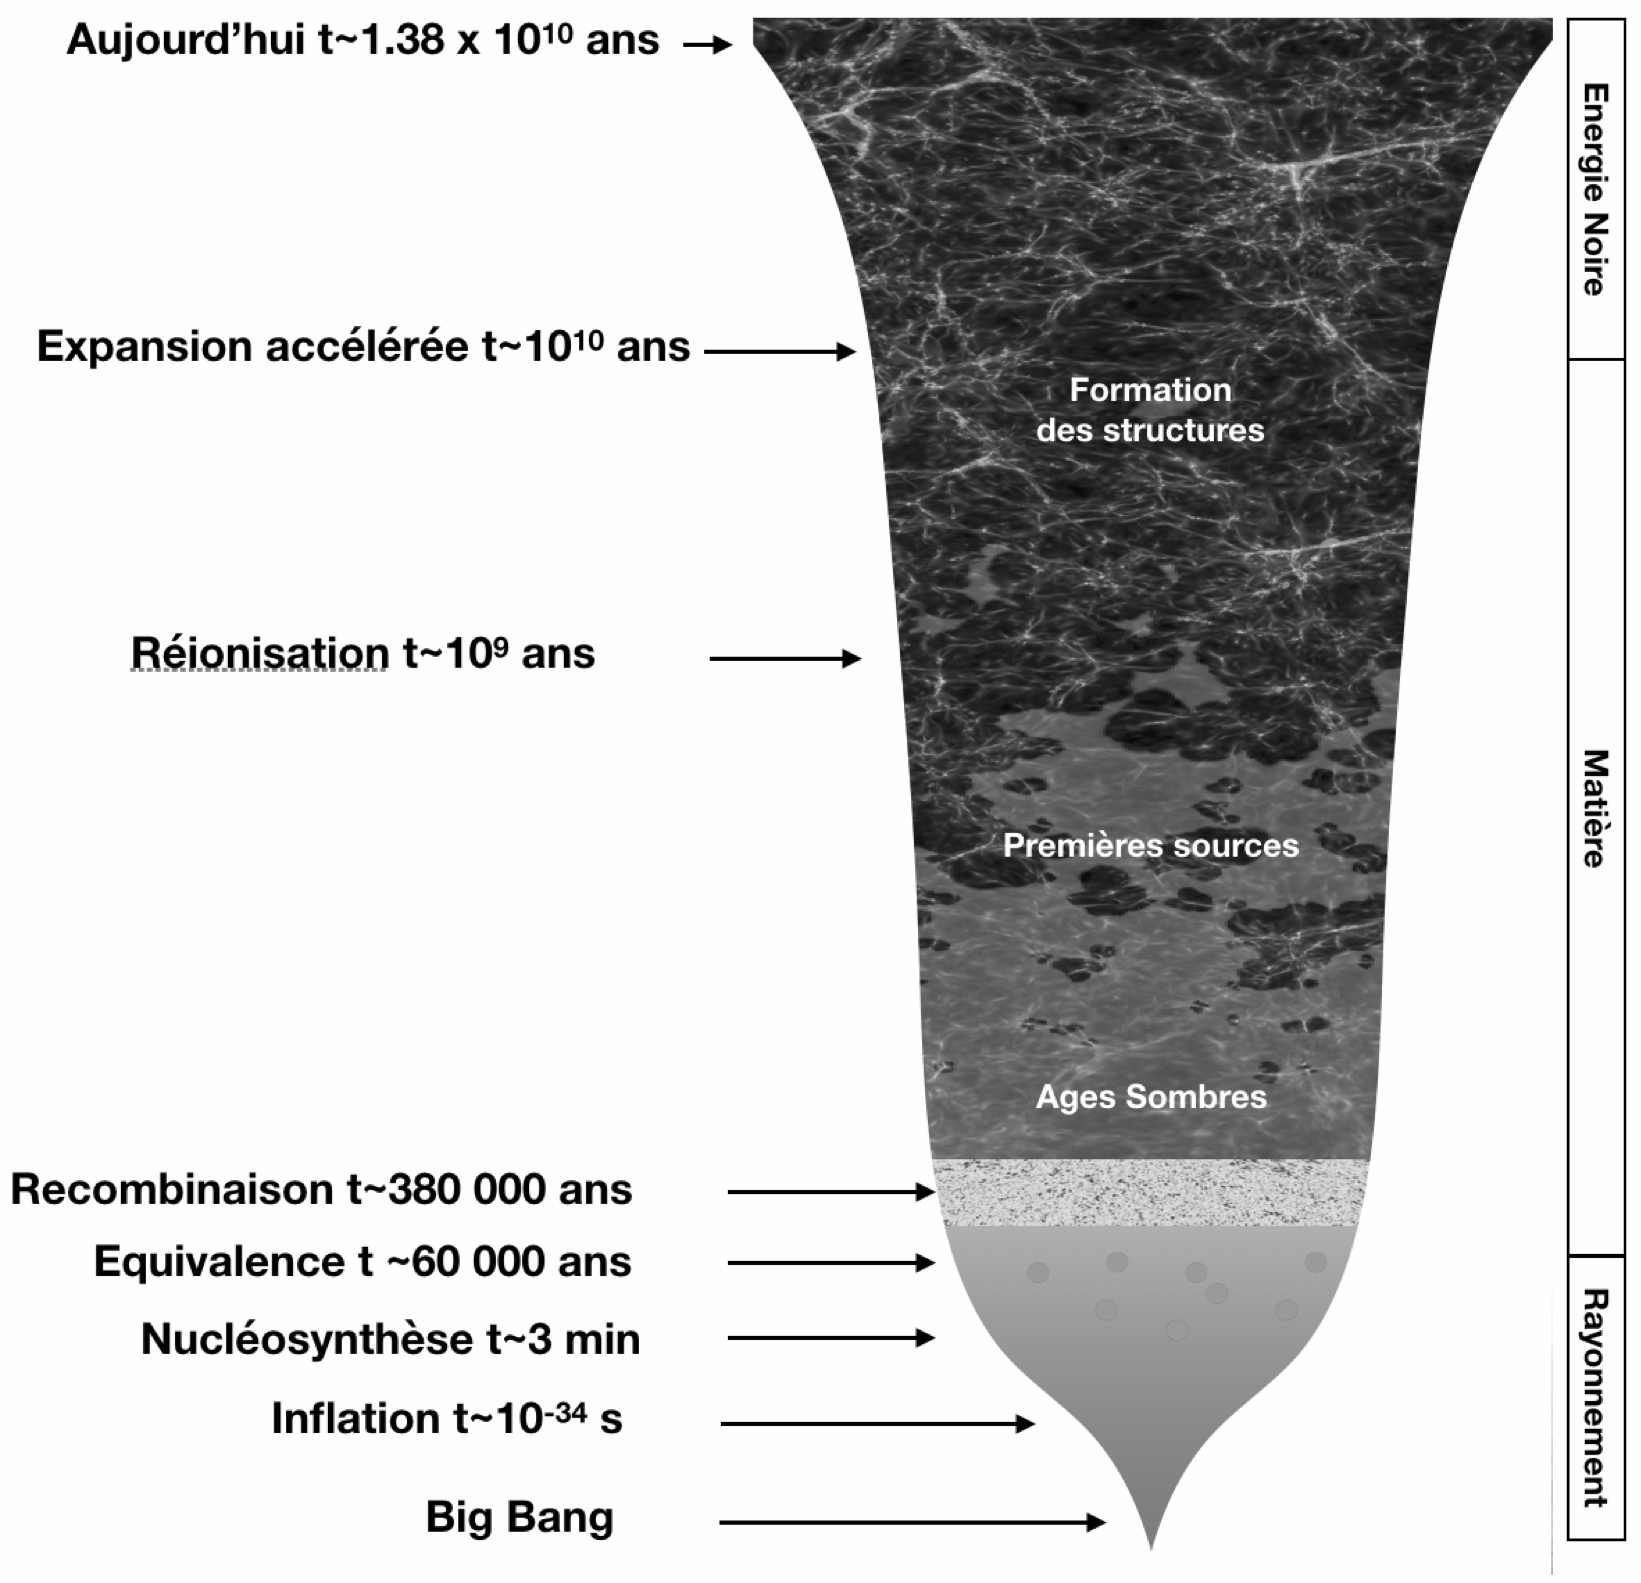
\includegraphics[height=10cm]{figs/timeline.png}
		\caption[Les grandes étapes dans l'histoire du cosmos]{Les grandes étapes dans l'histoire du cosmos. Cette frise couvre environ 13.8 milliards d'années d'évolution depuis le Big-Bang (à gauche) jusqu'à nos jours (à droite). \textit{Crédit:Planck-ESA}}
	\label{f:timeline}
\end{figure}

\newthought{Pour finir}, nous allons donner un cours descriptif des grandes étapes de l'histoire de l'Univers. Ces grandes étapes décrivent des processus physiques ou des transitions spécifiques qui opèrent à certains stades de l'évolution du cosmos et par extension sont aussi utilisés pour désignés des instants. Par exemple on parle de la réionisation pour désigner la fin du premier milliards d'années de l'Univers ou bien de l'inflation pour désigner ses premiers instants.

L'Univers a connu une phase extrêmement dense et chaude, il y a 13.8 milliards d'années. Nos théories actuelles ne nous permettent pas actuellement de remonter au delà d'un temps de Planck ($\sim 10^{-44}$ s), durée sur laquelle les effets de gravité quantique pourraient se manifester, mais à cette incertitude près, l'histoire de l'Univers débute à cette époque, nommée le \textit{Big-Bang}. A partir de cet instant, l'Univers va subir un effet d'expansion de l'espace et de baisse de sa température\index{température}. Dans le cadre du modèle cosmologique standard, les grandes étapes de son évolution sont les suivantes (cf. figure \ref{f:timeline}):
\begin{enumerate}
\item \underline{L'inflation} $t\sim 10^{-34}$ secondes\index{inflation} :  cette phase est encore spéculative et consisterait en une phase d'expansion accélérée de l'Univers dans ces instants quasi-initiaux. Si ce processus a bien eu lieu, il permettrait d'expliquer naturellement la grande homogénéité initiale de l'Univers, sa platitude et donnerait une origine quantique aux fluctuations initiales de matière qui sont à l'origine des grandes structures\index{grandes structures} actuelles de l'Univers. Ce processus aurait également été la source d'ondes gravitationnelles\index{ondes gravitationnelles} qui seraient toujours détectables et dont la découverte signerait la confirmation d'une phase d'inflation.
\item \underline{l'Univers primordial} $t<3$ minutes : au cours de cette époque l'Univers reste extrêmement chaud et dense. Il s'y déroule des processus à très haute énergie: plasma quark-gluons, confinement des quarks\index{quarks}, baryogénèse\index{baryogénèse} (i.e. l'annihilation matière anti-matière), découplage des neutrinos\index{neutrinos}, nucléosynthèse des éléments jusqu'à l'hélium\index{hélium}.
\item \underline{l'équivalence} $z=3400$ t=50 000 ans \index{equivalence@équivalence ! matière-rayonnement} l'Univers voit son bilan énergétique passer d'une domination par les espèces relativistes (le rayonnement) à une domination par la matière.
\item \underline{La recombinaison} $z=1100$ t=380 000 ans : l'Univers devient suffisamment froid (T=3000 K) et peu dense pour permettre la création d'atomes neutres et l'émission du fond diffus\index{fond diffus} cosmologique (CMB). 
\item \underline{les âges sombres} $1100>z>30$ \index{ages sombres@âges sombres} l'Univers est rempli de gaz froid et neutre. Le gaz se structure sous l'effet de la gravitation mais  n'est pas encore en mesure de former des étoiles\index{etoiles@étoiles}. 
\item \underline{la réionisation} $30>z>6$ le gaz parvient à des densité lui permettant de se convertir en étoiles. Ces étoiles vont émettre un rayonnement ionisant\index{ionisation} qui vont réioniser ($x_\mathrm{HI}\sim0.0001$) et réchauffer totalement l'Univers ($T\sim 10000$). C'est les stades initiaux de la formation des galaxies\index{galaxies}.
\item \underline{la formation des galaxies et des grandes structures} $30>z>0$ à partir de la formation des première étoiles vont se former les premières galaxies. Elles vont croître de façon hiérarchique \index{formation hiérarchique} par assemblage de petits objets pour former les plus gros, sous l'effet de processus d'instabilité gravitationnelle\index{instabilité gravitationnelle} dominés par une matière non baryonique. Les amas de galaxies\index{galaxies ! amas} vont apparaître vers $z=1$.
\item \underline{Accélération de l'expansion cosmique} $z\sim 0.3$, $t\sim 10$ milliards d'années. Le bilan énergétique de l'Univers devient dominé par l'énergie noire\index{energie noire @énergie noire}, induisant une expansion accélérée de l'Univers.
\item \underline{Aujourd'hui} $z=0$. L'Univers a 13.8 milliards d'années \index{age ! Univers}.
\end{enumerate}



%\chapter{Prélude: Cosmologie newtonienne\index{cosmologie Newtonienne}}

Ce chapitre est à la fois optionnel et indispensable : optionnel, car le reste de l'ouvrage n'en dépend pas et les quelques points qui y sont abordés sont décrits bien plus en détail dans les chapitres suivants. Il n'en reste pas moins indispensable en ce qu'il permet d'introduire facilement et simplement beaucoup de concepts utilisés couramment en cosmologie.

Ce prélude porte sur un modèle \textit{Newtonien} de cosmologie\index{cosmologie Newtonienne}. Ce modèle possède une portée limitée, mais permet une introduction progressive à certains concepts et à certains modes de raisonnements propres à la cosmologie. On discutera de sa validité et des hypothèses sous-jacentes en fin de chapitre, après en avoir exploré tous les recoins.

\newthought{Considérons} un «gaz de galaxies» \index{galaxie} homogène et isotrope au sein duquel on trace un volume sphérique de rayon $R$ et d'origine $O$. Au sein de ce volume, chacune de ces galaxies est repérée grâce à un rayon vecteur $r(t)$, variable au cours du temps (voir Fig. \ref{f:newton}). Ce modèle repose sur l'hypothèse que toutes ces galaxies vont voir leur position évoluer \textit{radialement} par rapport à $O$ suivant une loi homothétique:
\begin{equation}
r(t)=a(t)r_0.
\end{equation}
$r(t)$ est le rayon à un instant donné tandis que $r_0$ est le rayon mesuré pour chacune de ces galaxies à un instant arbitraire $t_0$. La dépendance temporelle est encodée dans le facteur d'échelle \index{facteur d'échelle}\sidenote{appelé aussi \textit{facteur d'expansion}}, $a(t)$. Ce dernier est un facteur sans dimension et dont on voit que par définition:
\begin{equation}
a(t_0)=a_0=1.
\end{equation}
Cet instant $t_0$ peut être choisi arbitrairement, mais il est d'usage de dire qu'il correspond au \textit{moment présent} : pour $t<t_0$ on regarde le système dans le passé et $t>t_0$ il s'agit du futur. De même, toute quantité indicée avec $0$ est prise à sa valeur aujourd'hui et par exemple $r(t_0)=r_0$.

\begin{figure}[htbp]
	\centering
		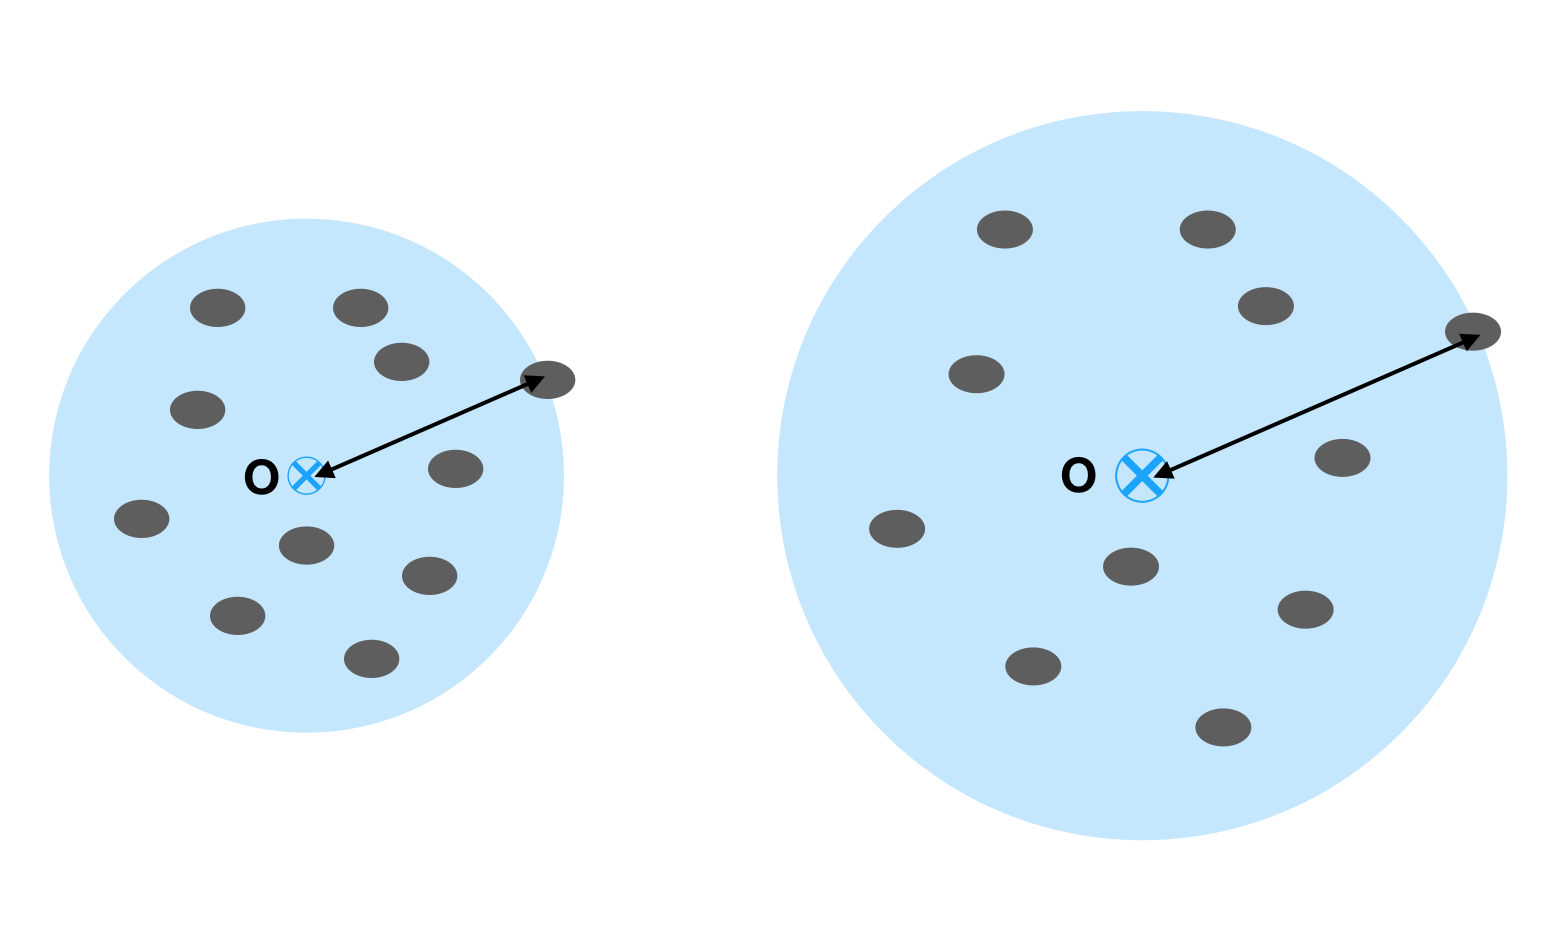
\includegraphics[height=6cm]{figs/newton.png}
	\caption[le modèle cosmologique Newtonien]{Le modèle Newtonien. La sphère représente une portion de gaz de galaxies, uniforme et isotrope centrée sur $O$. Seules quelques galaxies sont représentées ici sous forme d'ellipses : la plus éloignée d'entre elles fournit le rayon maximum de notre \textit{volume de contrôle} (montré ici sous la forme d'une flèche). Deux instants sont représentés ici, le temps s'écoulant de la gauche vers la droite et le volume subit alors une transformation homothétique. Notons que la galaxie la plus éloignée reste toujours la même à tous les instants.}
	\label{f:newton}
\end{figure}

Dès à présent, on peut constater que la notion de distance à l'origine n'est pas univoque : elle peut désigner la distance à un moment donné ou bien la distance variant au cours du temps. Pour lever cette ambiguïté, on appelle $r(t)$ \textit{la distance physique}\index{distance!physique}: à chaque instant elle représente l'intervalle qui sépare physiquement une galaxie de l'origine. De même on appelle $r_0$ la distance \index{distance!comobile} comobile : c'est la distance mesurée à un instant de référence $t_0$, mais on peut également la considérer comme une mesure effectuée dans un système de coordonnées en mouvement avec la matière (d'où le nom comobile). Enfin, le facteur d'expansion peut également être envisagé comme une mesure du rayon en unité du rayon comobile.

Si on considère maintenant le bord externe de notre volume de contrôle $R(t)$, celui-ci subit la même loi d'expansion\index{expansion} $R(t)=a(t)R_0$ \sidenote{se faisant on considère que ce rayon est «attaché» ou ancré à une galaxie, la galaxie la plus externe }. Ce volume de contrôle est sphérique, il évolue au cours du temps et son expression précise est:
\begin{equation}
V(t)=\frac{4\pi}{3} R(t)^3 = a(t)^3\frac{4\pi}{3} R_0^3= a^3 V_0.
\end{equation}
Son volume varie en $a^3$, comme tous les volumes attachés à de la matière. De même on peut aisément démontrer que sa surface varie en $a^2$ comme toutes les surfaces attachées à de la matière: dans les deux cas, la dépendance de ces quantités par rapport aux longueurs impose une certaine dépendance par rapport au facteur d'expansion. Ce type d'arithmétique est très fréquente en cosmologie et peut être aisément étendue à d'autres quantités, par exemple la densité de galaxies dans notre volume de contrôle:
\begin{equation}
n=\frac{N_\mathrm{gal}}{\frac{4\pi}{3} R(t)^3}=a^{-3} n_0.
\end{equation}
À cause de la dilution des longueurs et des volumes, la densité décroît au cours du temps avec une puissance $-3$ du facteur d'expansion. 

Notons dès à présent que la masse ou le nombre de galaxies restent invariants malgré l'évolution des distances. Dit autrement, le flux\index{flux} net au travers de la surface de contrôle est nul : aucune galaxie ne rattrape ou ne se fait dépasser par une galaxie initialement plus interne ou plus externe. En effet si $R_{0,a}<R_{0,b}<R_{0,c}$ alors à chaque instant $R_a<R_b<R_c$.

\newthought{La cinématique} de ce système mérite aussi d'être étudiée. La vitesse de fuite de chacune de ces galaxies est simplement donnée par:
\begin{equation}
\dot r= r_0 \dot a = \frac{\dot a}{a} r.
\end{equation}
À un instant $t$ donné, la vitesse de fuite\index{vitesse!fuite} est donc directement proportionnelle à la distance d'une galaxie : plus elle est éloignée de l'origine, plus elle s'en éloigne rapidement. Cela est cohérent avec l'absence de flux net au travers des limites du volume de contrôle. Le rapport de proportionnalité varie au cours du temps et est noté $H(t)$:
\begin{equation}
H(t)=\frac{\dot a}{a}.
\end{equation}
Dans ce cadre Newtonien, cette fonction est l'analogue à la fonction de Hubble \index{Hubble!fonction} que nous rencontrerons par la suite et nous retrouvons cette propriété observée dans notre univers. La vitesse de récession\index{vitesse!récession} des objets est proportionnelle à leur distance:
\begin{equation}
v=Hr
\label{e:hubblenewt}
\end{equation}
Cette loi dite \textit{de Hubble} est linéaire\index{linéaire}, ce qui a une grande importance. En effet, si la loi avait été quadratique ($v\sim r^2$) ou bien à vitesse de récession constante ($v\sim r^0$), on peut aisément montrer que l'homogénéité\index{homogénéité} initiale est détruite, ce qui n'est pas une propriété désirable de notre modèle d'Univers. Par ailleurs, on peut également démontrer que cette hétérogénéité serait dépendante du point de vue ou de l'origine utilisée, ce qui est une autre propriété indésirable. Cette loi de Hubble\index{Hubble!loi}, linéaire, est la seule qui permette de conserver une homogénéité et une égalité des points de vue.

\newthought{L'énergétique} du système nous est à présent accessible. Calculons la quantité d'énergie disponible dans ce gaz de galaxies, que ce soit sous forme cinétique ou potentielle. L' énergie cinétique \index{energie@énergie!cinétique} est obtenue en sommant l'énergie cinétique de chaque coquille de rayon $r$ et d'épaisseur $dr$ en récession \sidenote{$\rho$ désigne la densité massique de galaxies. Elle est indépendante de $r$, le système étant homogène}:
\begin{equation}
E_c=\int_0^R dE_c=\int_0^R \frac{1}{2}\rho  v^2(r) 4\pi r^2  dr.
\end{equation}
En utilisant la loi de Hubble (Eq. \ref{e:hubblenewt}) et la relation entre masse et densité, on obtient aisément l'expression suivante pour l'énergie cinétique totale du gaz en expansion\sidenote{M désigne la masse dans le volume de contrôle (conservée au cours du temps) et R le rayon de ce dernier}:
\begin{equation}
E_c=\frac{3}{10} M H^2 R^2.
\end{equation}
On y retrouve aisément une dépendance en vitesse au carré \sidenote{via le terme $Hr$}. De même l' énergie potentielle \index{energie@énergie!potentielle} totale de gravitation se trouve en intégrant l'énergie potentielle de chaque coquille \sidenote{l'énergie potentielle de gravitation est considérée nulle à l'infini. L'énergie potentielle d'une coquille de rayon $r$ ne dépend que de $M(<r)$, la masse à l'intérieur de son rayon. }:
\begin{equation}
E_p=\int_0^3 dE_p=-\int_0^R \frac{GM(<r)}{r}dm.
\end{equation}
Ayant $M(<r)=4/3\pi \rho r^3$ et $dm= 4\pi r^2 \rho dr$, on obtient:
\begin{equation}
E_p=-\frac{16 \pi^2 G}{3} \rho^2 \frac{R^5}{5}= -\frac{3}{5}\frac{GM^2}{R},
\end{equation} 
expression pour laquelle on retrouve bien une forme d'énergie potentielle de gravitation.

\section{Quelques éléments de dynamique}
Après avoir étudié ces quelques propriétés simples de notre modèle Newtonien, nous allons procéder à une première analyse de son évolution. Pour ce faire nous nous en tiendrons à une simple analyse énergétique. À partir des expressions des énergies cinétiques et potentielles, calculons l'énergie mécanique \index{energie@énergie!mécanique} totale de notre système auto-gravitant:
\begin{equation}
E=E_c+E_p=\frac{3}{10} M H^2 R^2 - \frac{3}{5}\frac{GM^2}{R}.
\end{equation}
Comme tout système auto-gravitant\index{système auto-gravitant}, sa stabilité nous est donnée par le signe de son énergie mécanique. Une énergie totale positive va conduire à un système libre, avec une expansion infinie (voire asymptotiquement infinie si elle est exactement nulle) tandis qu'une énergie négative correspond à celle d'un système lié, voué à s'effondrer au bout d'un certain temps.

\newthought{Quelle condition} faut-il satisfaire pour avoir un système lié ? Écrivons l'inégalité correspondante:
\begin{equation}
\frac{3}{10} M H^2 R^2 <\frac{3}{5}\frac{GM^2}{R}.
\end{equation}
Cette inégalité peut se réécrire sous la forme d'une condition sur la densité:
\begin{equation}
\frac{3H^2}{8\pi G}< \frac{M}{4/3\pi R^3}=\rho.
\end{equation}
Dit autrement si la densité de notre gaz de galaxies est supérieure à une certaine densité critique, le système est voué à atteindre un rayon limite et à s'effondrer. Cette densité critique \index{densité critique} est donnée par:
\begin{equation}
\rho_c =\frac{3H^2}{8\pi G}
\end{equation}
et correspond exactement à la densité critique obtenue par un traitement relativiste exact. De même on montrera qu'un gaz de galaxies sous- dense, avec $\rho< \rho_c$, n'est pas lié et  connaîtra une expansion illimitée. 

Compte tenu du rôle joué par cette densité critique, il est d'usage d'exprimer les densités massiques en unités de cette densité de référence. On parle alors de paramètre de densité \index{paramètre de densité} $\Omega$:
\begin{equation}
\Omega=\frac{\rho}{\rho_c}.
\end{equation}
Un système lié voué à l'effondrement équivaut à $\Omega>1$ tandis qu'un système en expansion infinie équivaut à $\Omega<1$. Le cas limite $\Omega=1$ correspond à un comportement asymptotique avec une expansion nulle à l'infini. À nouveau, cette relation sera très exactement retrouvée dans le cadre d'un traitement relativiste complet.

\section{Équation de Friedmann}

Ce paramètre de densité $\Omega$ intervient également dans l'équation différentielle qui régit l'évolution du facteur d'expansion $a(t)$\index{facteur d'échelle}. On rappelle que ce terme encode toute l'évolution temporelle des distances dans notre modèle Newtonien d'Univers, via la relation $r(t)=a(t)r_0$. Prenons la galaxie la plus lointaine\sidenote{ce choix est arbitraire, le même raisonnement peut être tenu pour n'importe quelle galaxie à l'intérieur du volume de contrôle}, dont la distance a l'origine est donnée par $R(t)$. Comme la mécanique newtonienne peut s'appliquer, le principe fondamental de la dynamique\index{principe fondamental de la dynamique} donne \sidenote{notons que le mouvement est purement radial en l'absence de mouvements initiaux tangentiels. $M(<R)$ désigne la masse à l'intérieur du rayon R et la force ressentie par la galaxie est celle crée par toute cette masse rassemblée en O.}:
\begin{equation}
\ddot R=-\frac{GM(<R)}{R^2}.
\end{equation} 
En l'absence de flux net au travers de $R$, la masse $M(<R)$ reste constante ce qui permet d'intégrer simplement en multipliant par $2\dot R$:
\begin{eqnarray}
2\dot R \ddot R &=& -2GM\frac{\dot R}{R^2}\\
\left(\frac{\dot R}{R}\right)^2&=&\frac{8\pi G}{3}\rho +\frac{K}{R^2}
\end{eqnarray}
où $K$ désigne une constante d'intégration. On reconnaît alors dans le terme de gauche le paramètre de Hubble $H=\dot a/a=\dot R/R$. Introduisons également la valeur de ce paramètre aujourd'hui $H_0=H(t_0)$ :
\begin{equation}
H^2=H_0^2(\frac{8\pi G}{3H_0^2}\frac{\rho_0}{a^3}+\frac{K}{(R_0  H_0)^2 a^2}).
\end{equation}
On reconnaît l'expression de la densité critique\index{densité critique} prise aujourd'hui $\rho_{c0}$ dans le terme lié à la densité de matière $\rho_0$. De plus le second terme lié à la constante d'intégration doit également être sans dimension et constant, à la dépendance en $a^{-2}$ près. Pour ces raisons, cette équation est généralement présentée sous la forme suivante:
\begin{equation}
H^2=H_0^2(\frac{\Omega_m}{a^3}+\frac{\Omega_K}{a^2}).
\label{e:friednewt}
\end{equation}
qui donne l'évolution du paramètre de Hubble\index{Hubble!fonction} au cours du temps \sidenote{via la dépendance temporelle en $a(t)$}, en fonction du contenu en masse, $\Omega_m$, de notre modèle d'Univers. La constante $K$ a généré un terme supplémentaire qui ne dépend que des conditions aux limites et qui doit satisfaire\sidenote{avec $H(a_0=1)=H_0$} :
\begin{equation}
\Omega_m+\Omega_K=1.
\end{equation}
Ce terme n'est pas libre et correspond à une quantité qui possède une dépendance en inverse de la longueur au carré\sidenote{par analogie avec le terme en densité qui varie en $a^{-3}$ alors que celui-ci varie en $a^{-2}$} : il correspond à un terme de courbure intrinsèque\index{courbure}. L'équation \ref{e:friednewt} contient toute l'information pour permettre de calculer $a(t)$, connaissant $\Omega_m$ et $H_0$: elle constitue l'une des formes de l'équation de Friedmann \index{equation@équation de Friedmann}.

\newthought{Prenons un Univers critique}: dans ce type de modèle, $\Omega_m=1$ et produit une dynamique que l'on sait être asymptotiquement en expansion pour un temps infini. L'équation \ref{e:friednewt} est alors très simple à intégrer à partir de \sidenote{ici on ne considère que la solution croissante, correspondant à l'Univers observé qui s'avère être en expansion}:
\begin{equation}
\dot a=\frac{H_0}{\sqrt{a}}
\end{equation}
ou bien
\begin{equation}
\sqrt{a}da=H_0 dt.
\end{equation}
En intégrant entre $t=0$ et un temps $t$ quelconque on obtient la loi d'expansion de ce modèle d'Univers:
\begin{equation}
a(t)=\left(\frac{3}{2}H_0 t\right)^{2/3}.
\end{equation}
On reconnaît une évolution temporelle lente asymptotique avec comme dérivées du facteur d'expansion:
\begin{eqnarray}
\dot a &\sim& t^{-1/3}\\
\ddot a &<&0.
\end{eqnarray}
La dérivée tend vers 0 à l'infini et la courbure est négative, donnant une expansion qui décélère : ce comportement est typique des Univers remplis de matière. Ce modèle est appelé modèle de \textit{Einstein-de Sitter} \index{Einstein- de Sitter}.

\newthought{L'âge de l'Univers}\index{age de l'Univers@âge de l'Univers} s'obtient également très facilement : il suffit de prendre le temps correspondant à un facteur d'échelle unité, c'est à dire le temps qu'il s'est écoulé depuis $t=0$:
\begin{equation}
t_0=\frac{2}{3H_0}.
\end{equation}
On constate alors que l'inverse du facteur de Hubble actuel est l'âge de l'Univers à un facteur proche de 1 près. De fait on nomme cette quantité le \textit{temps de Hubble}\index{Hubble!temps}\sidenote{Notons que la loi de Hubble $v=Hr$ suggérait déjà que $H$ constituait l'inverse d'un temps}:
\begin{equation}
t_H=H_0^{-1}.
\end{equation} 
Dans tous les modèles d'Univers, cette quantité constitue une bonne approximation de l'âge de l'Univers. De fait toute quantité temporelle qui est désignée comme étant de l'ordre du temps de Hubble \index{Hubble!temps} est implicitement désignée comme une quantité longue ou lente en évolution. C'est l'ordre de grandeur du temps caractéristique d'évolution de l'Univers.

Remarquons d'emblée que l'âge de l'Univers prédit par ce modèle simple est problématique. Pour une valeur typique de $H_0\sim 70$ km/s/Mpc \sidenote{correspondant à un temps de Hubble $t_H\sim 14$ milliards d'années}, le modèle d'Einstein-de Sitter conduit à un âge actuel d'Univers d'environ 9.2 milliards d'années or il existe des populations d'étoiles\sidenote{par exemple au sein d'amas globulaires\index{amas globulaire}} qui présentent des âges de plus de 13 milliards d'années. Ne pouvant avoir un Univers plus jeune que son contenu, il faut envisager autre chose qu'un Univers composé uniquement de matière avec une densité critique.

\section{Commentaire sur la validité du modèle}
À ce stade, on peut s'interroger sur les conditions d'applications de ce modèle Newtonien. Rappelons que nous considérons une sphère de «gaz» de galaxies dans un Univers homogène : il s'avère que dans certains cas, le traitement Newtonien est exact. En effet, faisons l'expérience de pensée qui consiste à retirer une sphère de matériau à cet ensemble homogène : quelle est la structure de l'espace-temps au sein de ce creux nouvellement créé ? La solution est donnée par le théorème de Birkhoff\index{théorème de Birkhoff} : l'espace-temps y est plat \sidenote{De la même façon, quel est le champ Newtonien de gravitation crée à l'intérieur d'une sphère creuse? D'après le théorème de Birkhoff, la réponse est un champ de gravitation nul, dont l'équivalent relativiste est une absence de courbure de l'espace-temps.}. Par conséquent lorsque la matière est remise dans ce creux la mécanique y est celle d'un espace plat\index{espace-temps!plat}, à savoir newtonienne.

Ceci n'est toutefois vrai qu'à certaines conditions, la première étant que la matière que nous remettons dans ce volume n'y courbe pas significativement l'espace afin que l'on puisse continuer à raisonner sans relativité générale. On peut par exemple imposer que l'énergie potentielle\index{energie@énergie!potentielle} de gravitation soit faible par rapport à son énergie de masse:
\begin{equation}
\frac{GM}{Rc^2}\ll 1
\end{equation}
Par ailleurs, il faut la taille de notre volume soit petite par rapport à l'horizon\index{horizon}, pour que les effets de propagation de l'interaction gravitationnelle \sidenote{qui se fait à la vitesse de la lumière} ne se fassent pas sentir:
\begin{equation}
\frac{RH}{c}\ll 1,
\end{equation}
ce qui est équivalent à considérer une vitesse de fuite très inférieure à la vitesse de la lumière. Donc de fait, le système ne peut être ni trop grand (pour éviter les grandes vitesses) ni trop petit (pour éviter les trop grandes densités). Par contre dans le cadre de ces hypothèses, le traitement est exact.

Une autre difficulté rencontrée par ce problème est qu'il est limité à l'action de la matière seule : qu'en est-il d'un modèle à l'intérieur duquel se trouve également du rayonnement ou bien toute autre forme d'énergie ? Le cadre Newtonien ne peut répondre à cette question or l'on comprend bien que ces autres types d'énergie doivent aussi contribuer à créer de la gravitation, comme indiqué par la relativité générale\index{relativité générale}. On peut faire appel de façon ad hoc à un résultat relativiste en disant que toute forme d'énergie va contribuer sous la forme d'une densité \textit{équivalente} de matière de la forme \sidenote{$\epsilon$ désigne la densité d'énergie associée à l'énergie en question et $P$ est sa pression}:
\begin{equation}
\tilde \rho= \frac{1}{c^2}(\epsilon + 3P).
\end{equation}
Dans le cas d'une matière froide\sidenote{sans pression}, on retrouve $\tilde \rho =\rho$. Pour le cas d'un gaz de rayonnement on peut démontrer que le la densité équivalente est $\tilde \rho =2\epsilon/c^2$. Par exemple pour un corps noir\index{corps noir} \sidenote{qui est l'exemple typique d'un gaz de photons fortement couplé avec la matière}, la densité d'énergie $\epsilon$ et la pression $P$\index{corps noir!pression} sont des fonctions simples de la température \index{corps noir!température} $T$\sidenote{ici $\sigma\sim 5.6\times10^{-8}Wm^{-2} K^{-4}$ désigne la constante de Stefan-Boltzmann}:
\begin{eqnarray}
\epsilon&=&\frac{4\sigma}{c} T^4\\
P&=&\frac{4\sigma}{3c} T^4.
\end{eqnarray}
Ces relations conduisent bien à la densité équivalente décrite ci-dessus. Toutefois, cette «astuce» ne permet pas d'expliquer quel rôle joue la pression et pourquoi elle contribue à modifier la dynamique de l'espace-temps. Cet aspect sera décrit plus en détail dans le chapitre suivant.


%%!TEX root = /Users/domaubert/Documents/Lectures/cosmologie/cosmo_main.tex

\chapter{Concepts Fondamentaux}

\section{Définition de l'Univers et de la Cosmologie}
\label{s:fond_def}
 Il faut 3 constituants pour définir complètement un Univers:
\begin{enumerate}
\item un contenu en énergie, qui peut être sous diverses formes,
\item un jeu de lois physiques qui régissent l'entrejeu des différentes énergies,
\item un espace-temps\index{espace-temps}, qui est la scène sur laquelle cet entrejeu prend place.
\end{enumerate} 
L'enjeu de la \textit{cosmologie} est précisément d'étudier le contenu, les lois physiques et la structure de l'Univers. Par conséquent la cosmologie est liée aux aspects théoriques les plus fondamentaux de la physique mais également à des problèmes astrophysiques et il existe plusieurs manières de faire de la cosmologie. On cherchera par exemple à déterminer quelles sont les lois à l'œuvre dans le cosmos (point 2) , ce qui est davantage du domaine de la physique théorique, ou bien à déterminer les paramètres (point 3)  qui caractérisent la structure spatio-temporelle (e.g. sa forme ou bien son histoire) de l'Univers comme en cosmologie observationnelle. De même comprendre comment les différentes formes d'énergie (matière, lumière, etc...) s'organisent ou évoluent au cours du temps (point 1) (e.g. comment les grandes structures de l'Univers se mettent en place) permet d'avoir un éclairage sur les deux autres aspects du problème cosmologique.

\section{Principe Cosmologique}\index{principe cosmologique}
L'objectif de la cosmologie est ambitieux et cette ambition n'est pas sans obstacles. L'un des problèmes les plus importants est notre incapacité à garantir que ce que nous observons autour de nous reste valable à l'échelle du cosmos, \textit{y compris dans les régions de l'Univers qui nous serons à jamais inaccessibles}. Par exemple, rien ne garantit absolument que la neutralité électrique\index{neutralité électrique} soit vraie dans tout le cosmos ou bien que la densité de matière mesurée dans notre Univers observable soit effectivement celle de l'Univers entier\sidenote{on distingue parfois \textit{Cosmos} et \textit{Univers}, où le Cosmos est la sous-partie de l'Univers qui nous est accessible. Par simplicité, aucune différence ne sera faite entre les deux termes dans cet ouvrage.}. Aujourd'hui, il ne viendrait à l'idée de personne d'attribuer au cosmos une densité égale à celle de la Terre, pour autant c'est peu ou prou ce que nous faisons en cosmologie. 

Pour autant, \textit{nous n'avons pas le choix}. Par définition, il est impossible de connaître les propriétés de régions dont on ne peut extraire de l'information et toujours par définition, il existe de telles régions dans l'Univers. Quelle option reste-t-il à la personne désireuse de faire de la science à l'échelle de l'Univers, si ce n'est de supposer que ce qui nous est accessible est valide dans tout le cosmos ? Aucune : en l'absence d'une telle hypothèse, il est tout simplement impossible de faire de la science avec l'Univers.

Cette supposition est à la base du \textit{Principe Cosmologique}\index{principe cosmologique}. Si nous revenons sur les 3 constituants définis en début de chapitre, il est aisé de reconnaître que cette supposition implique que le contenu universel en énergie doit être le même que celui que nous constatons autour de nous. De même, la structure spatio-temporelle universelle doit être la même que celle que nous constatons dans l'Univers observable. Toutefois cette hypothèse "universaliste" implique également que nous supposons que les même lois de la nature s'appliquent dans tout le cosmos, y compris dans les régions qui nous sont inaccessibles ou pour lesquelles l'information n'est pas extractible. Le \textit{Principe Cosmologique} que nous retiendrons est le suivant : le contenu en énergie de l'Univers, sa structure spatio-temporelle et les lois qui y opèrent sont les même partout et par conséquent sont celles que nous constatons autour de nous. Notons tout de suite que cette universalité des composants s'applique aux échelles pertinentes pour la cosmologie et n'empêche pas des départs locaux aux valeurs universelles.

\subsection{Tautologie}

A ce stade, il nous semble que la cosmologie peut être définie par une tautologie~: \textit{la cosmologie est la science qui met le principe cosmologique à l'épreuve.} Si nous nous retrouvons dans une situation qui reste inexplicable dans ce que nous croyons être le jeu universel de contenu énergétique, spatio-temporel et "législatif" de l'Univers, alors les options sont réduites:
\begin{itemize}
\item soit nous continuons de croire que le principe cosmologique reste valide et c'est le détail de son contenu qui doit être révisé. Par exemple on modifiant les lois de la physique pour qu'elles rendent compte des nouveaux phénomènes tout en continuant à être une bonne description des processus locaux. C'est la voie scientifique standard.
\item soit nous renonçons au principe cosmologique et donc à l'universalité de ses composants et nous renonçons en même temps à l'ambition de décrire tout l'Univers avec la science que nous connaissons.
\end{itemize}

\subsection{Principe cosmologique pragmatique}
Le principe cosmologique est souvent décliné dans une version plus pragmatique qui est la suivante:
\begin{enumerate}
\item la gravitation est correctement décrite par la théorie de la relativité générale d'Einstein \index{relativité générale},
\item l'Univers est homogène et isotrope\index{homogénéité}\index{isotropie}.
\end{enumerate}
Le point 2 revient à appliquer au cosmos ce que nous voyons de l'état de l'Univers autour de nous (contenu, géométrie, évolution etc...). Le point 1 revient à définir les lois universelles de la gravité~: une emphase particulière est mise sur cette interaction\sidenote{On rappelle qu'on distingue 4 interactions fondamentales \index{interaction fondamentale} : la \textit{gravitation}, la \textit{force électromagnétique} et les deux forces corpusculaires\textit{ fortes} et \textit{faibles}.} car elle est la seule qui \textit{in fine} est toujours de portée infinie et donc cosmologique. Par ailleurs, une fois la théorie de relativité générale\index{relativité générale} choisie comme description correcte de la gravité, le point 2 a des conséquences sur les régimes qui vont être explorés avec cette théorie.

\section{Relativité Générale: notions}
La gravitation\index{gravitation} est centrale à l'étude de la cosmologie car elle est la seule "force"\index{force} dont l'action ne peut être écrantée et dont la portée soit infinie \sidenote{les forces corpusculaires sont de courte portée tandis que la force électromagnétique est en pratique toujours écrantée car une charge n'est jamais isolée de charges opposées sur les échelles qui nous intéressent}. De fait, elle est la seule force qui soit effective lorsque des échelles cosmologiques sont abordées. De plus la gravitation peut être décrite comme la manifestation des propriétés de l'espace-temps. Or il s'avère que la structure spatio-temporelle de l'Univers n'est pas triviale comme l'indique par exemple le phénomène d'expansion de l'Univers. Par conséquent l'observation de l'expansion du cosmos nous dit également des choses sur la façon dont la gravitation est à l'œuvre dans le cosmos. Compte tenu du rôle central de la gravitation pour les études cosmologiques, nous allons faire un aperçu de la théorie de la relativité générale\index{relativité générale} et sur son application dans le cadre cosmologique\sidenote{le lecteur intéressé pourra par exemple se reporter à l'excellent ouvrage d'introduction \textit{A first course in general relativity} par B. Schutz.}.

\subsection{Principe d'équivalence}
Le principe d'équivalence\index{principe d'équivalence} existe sous forme de différentes saveurs. La plus triviale est la suivante, où l'on considère le principe fondamental de la dynamique :
\begin{equation}
\frac{F_z}{m_i}=\ddot z.
\end{equation}
Ici l'on explique que l'accélération\index{accélération} suivant la direction z est \textit{proportionnelle} à la force appliquée au système étudié et \textit{inversement proportionnelle} à un coefficient, que l'on nomme \textit{masse inertielle}\index{masse inertielle}. Par conséquent, deux systèmes soumis à la même force vont réagir différemment selon les valeurs du coefficient $m_i$ qui les caractérisent. Intuitivement on comprend assez rapidement que ce coefficient est lié à la quantité de matière que le système possède, d'où son qualificatif de masse~: soumis à la même force, un système fortement chargé en matière réagira moins qu'un système ayant une quantité de matière plus faible. Maintenant considérons l'expression de $F_z$ si cette force se trouve être une force de pesanteur \sidenote{c'est à dire le poids}:
\begin{equation}
F_z=m_g g
\end{equation}
où g est la norme du champ de pesanteur. Cette force $F_z$ est d'autant plus forte que le coefficient $m_g$ est important~: ce coefficient caractérise également la quantité de matière dans le système et un système avec une grande quantité de masse va naturellement avoir une valeur élevée de $m_g$ et donc une pesanteur importante. Cette masse $m_g$ est aussi dénommée \textit{masse grave}\index{masse grave}.

A ce stade, nous avons donc deux coefficients qui tracent la quantité de matière dans un système physique:le premier $m_i$ lié aux équations de la dynamique, et sans aucune référence à priori à une force de pesanteur (ou de gravitation),  et le second $m_g$ qui lui pour le coup est complètement lié à la présence d'un champ de pesanteur. Il faut alors se rappeler qu'à priori, \textit{rien} ne nous informe d'une quelconque relation quantitative entre les deux et qu'il faut postuler une éventuelle relation entre les masses inertielles et graves.

Toutefois, l'expérience nous indique que tous les systèmes soumis à un champ de pesanteur donné semblent posséder la même accélération $\ddot z$ et ceci quelles que soient leurs masses inertielles et graves. Ceci implique que $m_g\sim m_i$. Plutôt qu'une vague égalité, \textit{le principe d'équivalence} stipule une exacte identité entre ces deux quantités:
\begin{equation}
m_g=m_i.
\end{equation}
Cette égalité est fortement suggérée par l'expérience, mais ne peut être démontrée comme étant absolument valide \sidenote{actuellement les mesures expérimentales excluent toute différence relative entre les 2 masses supérieure à $10^{-12}$}. Selon ce principe, la quantité de matière intervient au travers d'une valeur unique qui est \textit{la masse} $m=m_g=m_i$. On peut noter dès à présent que cette égalité confère à la gravitation un rôle spécial~: la masse \textit{inertielle} est liée à la loi décrivant la dynamique des systèmes, y compris en l'absence de gravitation. Par exemple, une particule chargée dans un champ électrique verra son accélération modulée en $q/m_i$. La force électrostatique, comme toutes les autres forces subit l'impact de ce coefficient d'origine dynamique. D'après le principe d'équivalence\index{principe d'équivalence}, la gravitation quant à elle possède \textit{dans sa propre expression} ce même coefficient, avant expression d'un quelconque problème dynamique. Elle dispose donc de façon innée d'une sorte d'élément d'information sur la façon dont la dynamique est régie, information que ne possèdent pas les autres interactions.

\subsection{Référentiel inertiel}
L'équivalence entre masse grave et inertielle a plusieurs conséquences. Comme déjà mentionné, elle permet de rendre compte de l'universalité de l'accélération de systèmes différents dans un même champ de pesanteur. C'est la fameuse expérience de la tour de Pise où des masses différentes lâchées de la même hauteur parviennent au sol au même instant car étant accélérées exactement de la même façon. Il en découle également que si l'on fait le choix d'étudier la chute libre\index{chute libre} de plusieurs objets dans un référentiel lui même en chute libre, ces objets apparaissent tous comme en "flottaison" comme si l'on avait annulé la gravitation dans ce référentiel\index{référentiel} et ceci même si ils sont tous très différents. A nouveau cela n'est possible que parce que la chute libre dans un champ de pesanteur est la même quel que soit l'objet considéré. 

\begin{figure}[htbp]
	\centering
		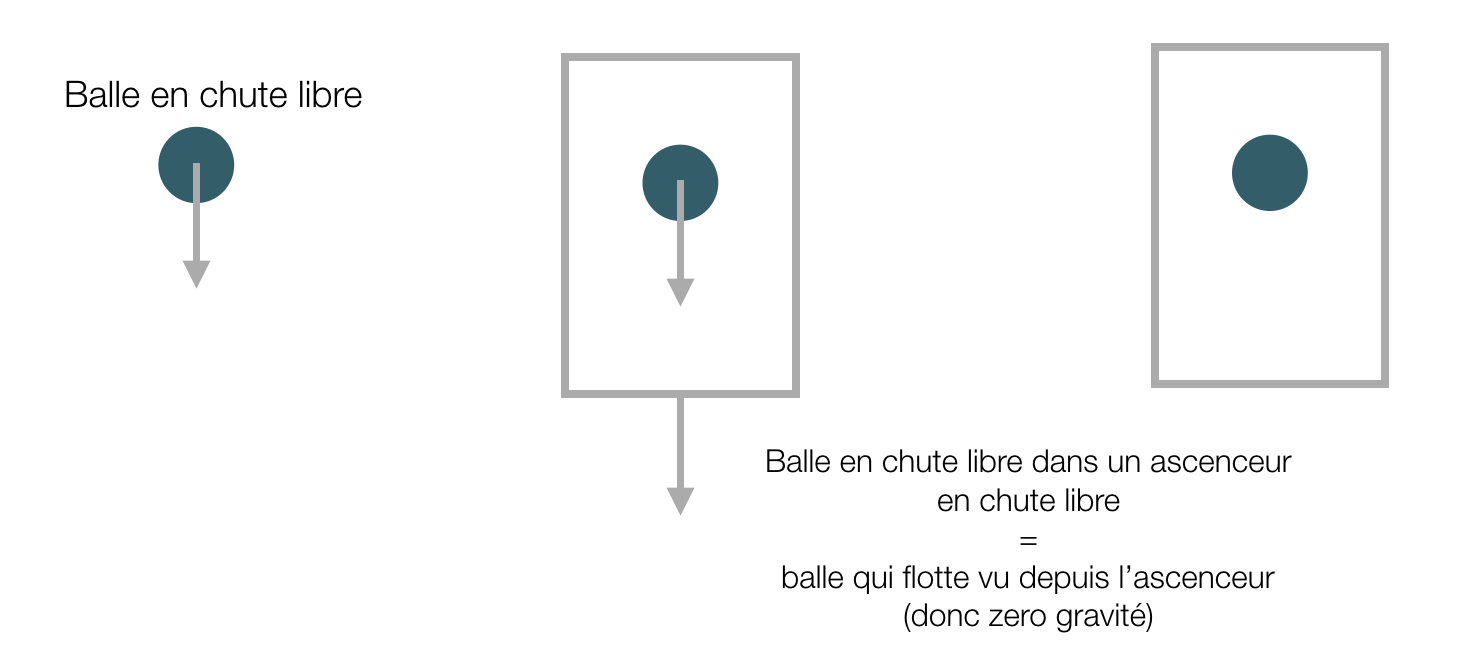
\includegraphics[height=10cm]{figs/ascenceur.png}
	\caption[Annulation du champ de pesanteur][-2cm]{Dans cette expérience de pensée, on considère une balle en chute libre dans un champ de pesanteur. Si on encage cette balle dans un ascenceur lui-même en chute libre, on crée un référentiel concrétisé par les parois de l'ascenseur, à l'intérieur duquel la balle 'flotte'. Dans ce jeu de coordonnées précis, on annule la gravitation : un observateur à l'intérieur de l'ascenseur est incapable de dire si on a éteint la gravité, ou bien si il se trouve dans un ascenceur en chute libre. Notons que comme tous les objets tombent à la même vitesse, l'observateur ne peut pas se renseigner en faisant la même expérience avec des objets divers : tous les objets, quelles que soient leurs masses et leurs compositions vont flotter de la même manière. }
	\label{f:ascenceur}
\end{figure}


Ce type de référentiel est appelé \textit{référentiel inertiel}\index{référentiel inertiel}. Généralement un tel référentiel ne peut être construit que localement et par exemple dans un champ de pesanteur radial, il est possible de construire une collection de référentiel inertiels qui annuleront la gravité localement mais aucun de ces référentiels ne peut annuler globalement le champ de pesanteur. A ce titre il est usuel de se référer à ce type de référentiel sous l'appellation \textit{référentiel localement inertiel}. Cette possibilité d'annuler localement la gravité est intrinsèquement lié à l'égalité $m_i=m_g$. Ce lien est si fort que l'on va considérer que \textit{la possibilité d'annuler la gravitation par un choix approprié de référentiel local est aussi un énoncé du principe d'équivalence}. 

\begin{figure}[htbp]
	\centering
		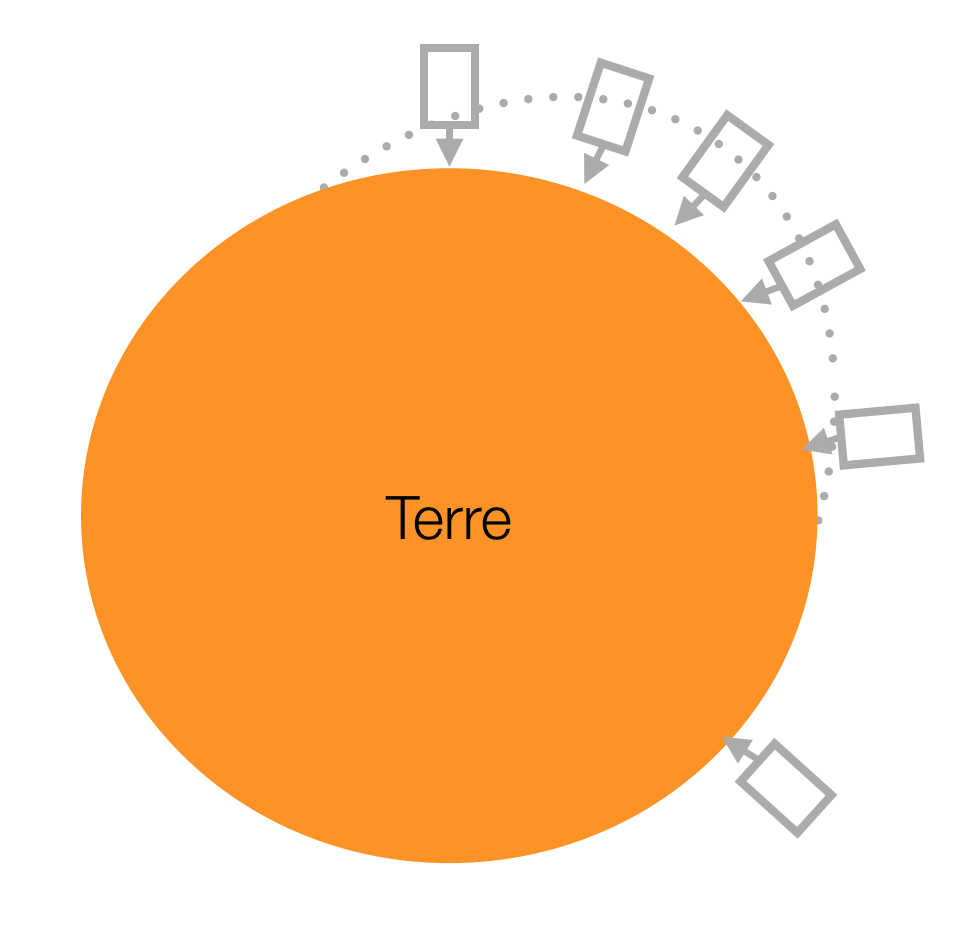
\includegraphics[height=10cm]{figs/ascradial.png}
	\caption[Référentiels localement inertiels]{Tous ces ascenseurs en chute libre, \textit{localement}, vont annuler le champ de pesanteur. En revanche, ils sont tous orientés différemment, suivant le champ de pesanteur local : on ne peut pas construire un système de référence global qui annule tous les champs de gravité. Ces référentiels inertiels sont locaux.}
	\label{f:ascradial}
\end{figure}

De fait, cette approche renverse le point de vue habituellement adopté sur le comportement mécanique des objets. Le point de vue newtonien classique consiste à supposer l'existence d'un champ de pesanteur qui va par exemple 'tordre' la trajectoire d'un objet initialement rectiligne en une parabole \sidenote{c'est le cas par exemple de la trajectoire balistique standard en $z(t)=-\frac{g t^2}{2}+V_0 t +x_0$.}. Dans l'approche relativiste, la trajectoire d'un système est toujours rectiligne dans les référentiels localement inertiels : en effet, en l'absence de pesanteur, le système se déplace toujours en ligne droite. Mais comme les référentiels ne sont pas tous 'alignés' les uns avec les autres, la trajectoire apparaît comme 'tordue' : les systèmes se propagent en ligne droite dans des systèmes de références qui ne sont pas 'alignés', créant ainsi toutes les variétés de trajectoires que nous connaissons. 


Notez qu'à l'aide d'un choix approprié de référentiel on peut également créer de la gravité. Si des systèmes libres sont placés dans un référentiel uniformément accéléré, ils percevront leur mouvement relatif comme induit par une force de gravitation. \textit{De façon générale il est impossible localement de distinguer un référentiel uniformément accéléré d'un champ de gravitation.}


\subsection{Qu'est-ce que la gravitation ?}
A nouveau, on peut créer ou "détruire" un champ gravitationnel par un choix approprié de référentiel. Or un référentiel pourrait se résumer à un ensemble de règles étalons et d'horloges ayant un certain comportement donc à un objet qui n'a qu'une nature géométrique et non pas physique. A partir de cette constatation, il est tentant de considérer alors que la gravitation n'est qu'une manifestation géométrique de l'espace dans lequel évoluent les systèmes. C'est le choix que fait la théorie de la relativité générale\index{relativité générale} (RG par la suite), où la gravitation n'est pas une force à proprement parler mais davantage une manifestation de la géométrie\index{géométrie} de l'espace-temps\index{espace-temps}. En RG, les systèmes se déplacent librement dans une géométrie qui, si elle est non triviale, produit des effets qui peuvent être interprétés comme le produit d'une interaction. A ce titre on peut dire que \textit{la gravitation n'existe pas}, elle n'est qu'une interprétation d'un effet de nature fondamentalement géométrique. 

Ainsi, on verra par la suite que c'est la courbure de cette géométrie qui produit les effets gravitationnels \sidenote{mathématiquement, cela se manifeste par des dérivées secondes de la géométrie par rapport aux variables qui décrivent l'espace-temps}. A l'inverse, une géométrie sans courbure\index{courbure}, i.e. une géométrie plane, produit un environnement sans effets de gravitation. Or il est aisé d'imaginer qu'il est toujours possible de trouver \textit{localement} un jeu de coordonnées qui rendent une géométrie plane, i.e. une transformation \textit{locale} qui permette de détruire la gravitation. Par analogie, une fonction régulière peut être approximée comme une collection de tangentes sur lesquelles il n'y a pas de courbures et qui localement sont des représentations exactes de la fonction originale. C'est une manifestation du principe d'équivalence~:\textit{il est toujours possible de trouver une transformation locale qui rende la géométrie de l'espace-temps plane}. Plus précisément c'est parce que l'on considère la gravitation comme étant de la géométrie que le principe d'équivalence se trouve naturellement réalisé.

Cette capacité à créer un jeu de coordonnées qui puisse annuler la gravitation est d'une importance majeure, pour la physique en général. En effet, comment faire pour faire de la physique en présence d'un champ de gravitation ? Il suffit d'annuler la gravitation, par un choix approprié de système de référence, pour retomber sur le cas sans gravitation et que généralement on arrive à formuler. D'un point de vue technique, si l'on parvient en l'absence de gravitation à exprimer les lois dans la nature dans une formulation qui s'accommode de changements de référentiels 'propres' \sidenote{on parle de formulation \textit{covariante}}, nous sommes capables de les exprimer en présence de gravitation car il existe toujours un 'point de vue' qui permet d'annuler ses effets. C'est le cas par exemple des lois de l'électromagnétisme, qui possèdent une telle formulation.

Cette vue de la gravité comme géométrie de l'espace-temps est l'école classique d'interprétation de la RG. Elle n'est toutefois pas sans poser problème par exemple si l'on cherche à quantifier la gravitation\index{gravitation quantique}. Si cette dernière est pure géométrie alors on peut arguer qu'il n'y a rien à quantifier et par exemple il n'y a pas de raison à priori d'invoquer l'existence d'un boson\index{boson} porteur de l'interaction, coupant court à toute tentative de quantification et donc d'unification. Si l'on estime que la quantification\index{quantification} est nécessaire alors la vision géométrique n'est qu'une interprétation, certes très puissante, d'un processus qui n'est pas pure géométrie. Dans ce cadre le principe d'équivalence devient prééminent: il faut le supposer réalisé par un mécanisme encore inconnu et sa réalisation conduit à une possible interprétation géométrique \sidenote{c'est par exemple l'approche adopté par S. Weinberg dans le livre \textit{Gravitation \& Cosmology} }. L'approche classique vue précédemment raisonne de façon inverse.

\subsection{Espace-temps et Métrique}
La théorie de la relativité générale décrit la gravitation comme une manifestation de la géométrie de l'espace-temps\index{espace-temps}. Cet espace temps possède 4 dimensions, une de temps et trois d'espace. L'outil mathématique permettant de décrire cette géométrie est la géométrie différentielle\index{géométrie différentielle}. Une quantité centrale est \textit{la métrique}\index{métrique}~: fondamentalement elle est l'outil qui permet de calculer des distances (des produits scalaires) dans une géométrie arbitraire. En notation d'Einstein\index{notation d'Einstein}\sidenote{la notation d'Einstein consiste à omettre le signe de sommation sur les indices répétés. Par exemple $g_{\alpha\beta} x^\alpha =\sum_\alpha g_{\alpha\beta} x^\alpha$ }, le calcul d'une distance\index{distance} s'écrit de la façon suivante :
\begin{equation}
ds^2=g_{\mu\nu}dx^\mu dx^\nu,
\label{e:scal}
\end{equation}
où les indices $\mu,\nu$ courent sur les indices des coordonnées, $ds^2$ est un scalaire donnant la distance couverte par un intervalle\index{intervalle} $(dx^0,dx^1,dx^2,dx^3)$. La quantité $g_{\mu\nu}$ est la métrique et permet de relier la distance aux composantes de l'intervalle\index{intervalle}. Si la géométrie est plane, la métrique aura une certaine forme et si la géométrie est courbe et complexe, cette expression sera différente. En géométrie euclidienne\index{géométrie!euclidienne} plane à 3D le calcul de distance est le suivant:
\begin{equation}
ds^2=(dx^1)^2+(dx^2)^2+(dx^3)^2.
\end{equation} 
En géométrie de Minkowski\index{géométrie!Minkowski}, correspondant à l'espace-temps plat utilisé par la relativité restreinte, le calcul devient
\begin{equation}
ds^2=(dx^0)^2 -((dx^1)^2+(dx^2)^2+(dx^3)^2)
\end{equation} 
où $dx^0=cdt$ est la composante liée au temps. L'expression générale est elle donnée par Eq. \ref{e:scal}.

Cette métrique synthétise la structure spatio-temporelle de la \textit{variété} que l'on cherche à étudier. Pour faire de la cosmologie, il faut ainsi se doter d'une telle métrique, la plus à même de représenter ce que l'on croit être les caractéristiques génériques du cosmos.

\subsection{Métrique de Friedmann-Robertson-Walker}
En se rappelant l'énoncé du principe cosmologique\index{principe cosmologique} pragmatique, la métrique devant servir à décrire l'Univers doit refléter les propriétés d'homogénéité et d'isotropie\index{homogénéité}\index{isotropie}. La métrique la plus générique satisfaisant ces contraintes est la métrique de Friedmann-Robertson-Walker (FRW)\index{Friedmann-Robertson-Walker!métrique}. A l'aide de celle-ci, l'intervalle de distance 4D est donné par:
\begin{equation}
ds^2=c^2dt^2-a(t)^2(\frac{dr_0^2}{1-Kr_0^2}+r_0^2d\theta^2+r_0^2\sin^2\theta d\phi^2).
\label{e:FRW}
\end{equation}
On note que cette métrique fait usage d'un système de coordonnées sphériques $(r_0,\theta,\phi)$ pour sa partie espace. On note également que par rapport aux exemples Euclidien et Minkowskien, FRW couple explicitement les parties temporelles et spatiales, via le facteur d'expansion \index{facteur d'échelle} $a(t)$ \sidenote{appelé aussi facteur d'échelle}.  

$r_0$ est une \textit{distance comobile}\index{distance!comobile}~: c'est une coordonnée de nature spatiale et indépendante du temps. Ici elle désigne une distance radiale prise à partir de l'origine du système de coordonnées et est également prise en compte pour calculer les contributions à l'intervalle des séparations angulaires $d\theta$ et $d\phi$. Le paramètre $K$ est un paramètre \textit{de courbure} auquel on peut éventuellement associer un rayon de courbure\index{courbure} $R_K=K^{-1/2}$ \sidenote{une simple analyse dimensionnelle montre par exemple que $Kr_0^2$ doit être sans dimension}.

Si l'on considère deux évènements sur une même ligne de visée\index{ligne de visée} (donc avec $d\theta=d\phi=0$), l'intervalle peut se représenter sous une forme
\begin{equation}
ds^2=c^2dt^2-dr^2,
\end{equation}
avec 
\begin{equation}
dr=\frac{a(t)dr_0}{\sqrt{1-Kr_0^2}}.
\label{e:phydist}
\end{equation}
Ici $dr$ désigne la distance \textit{physique}\index{distance!physique} de la partie spatiale (donc 3D) de l'intervalle que nous étudions. Cette distance dépend du temps, donc de l'instant considéré, et est modulé par une éventuelle courbure. A proximité de l'origine ($r_0\rightarrow 0$) ou dans des régimes de très faible courbure ($R_K\rightarrow\infty$ ou $K\rightarrow 0$), distance physique et distance comobile sont directement reliées par :
\begin{equation}
dr=a(t)dr_0.
\end{equation}

\begin{figure}[htbp]
	\centering
		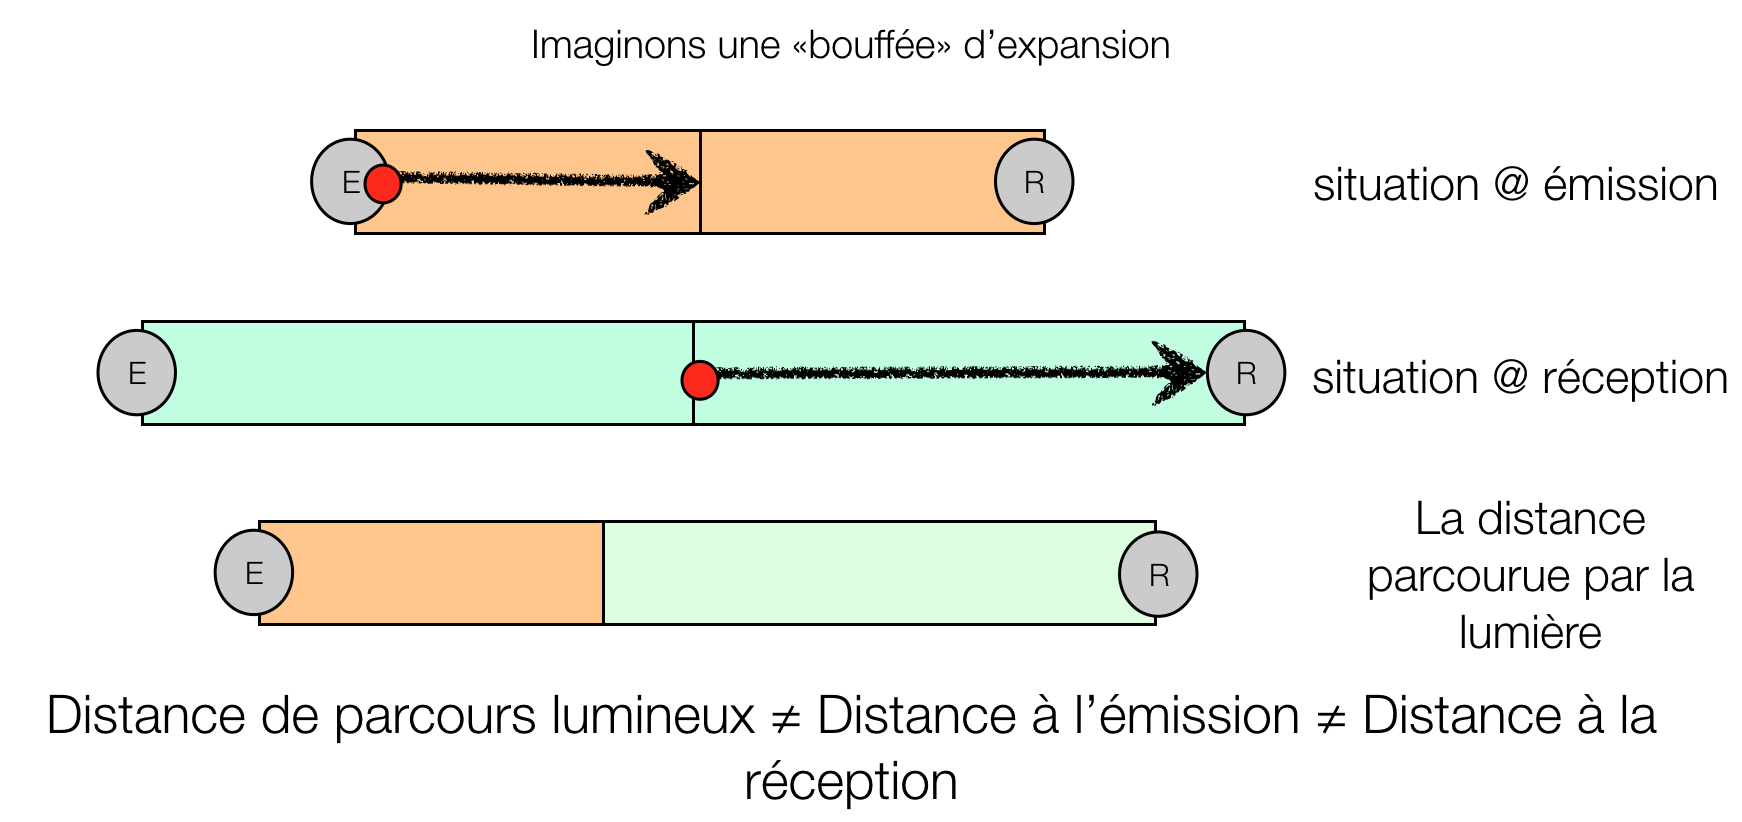
\includegraphics[height=10cm]{figs/dlum.png}
	\caption[Distance de parcours lumineux]{On considère un photon émis en E et reçu en R. Pour simplifier, les distances subissent une expansion instantanée au moment où le photon a parcouru la moitié de la distance initiale entre E et R. 3 distances peuvent être également considérées dans cette expérience de pensée : la distance physique entre E et R \textit{à l'émission} (représentée par 2 blocs courts), la distance physique entre E et R \textit{à la réception} (représentée par 2 blocs longs) et la distance effectivement parcourue par le photon entre l'émission et la réception (représentée par un bloc long et un bloc court). Ces trois distances sont différentes dans un Univers non statique. }
	\label{f:dlum}
\end{figure}

Là où la distance comobile était une quantité statique, la distance physique est une quantité évolutive, dont la dépendance temporelle est encodée par le facteur d'expansion $a(t)$. Notons que si l'on considère le parcours d'un photon\index{photon} sur un intervalle infinitésimal ($t$ est alors quasi constant et $r_0<<1$) alors $dr=cdt$ et la distance physique est celle effectivement parcourue par le rayon lumineux. Considérons à présent un intervalle non-infinitésimal : si la géométrie intrinsèque de l'Univers est plane, nous avons $K=0$ et la distance de parcours lumineux \index{distance de parcours lumineux} \textit{dans ce cas précis} vaut 
\begin{equation}
D_L=\int_{t_e}^{t_r} dr=\int_{t_e}^{t_r}a(t)dr_0,
\end{equation}
où $t_e$ et $t_r$ désignent les instants d'émission et de réception de ce photon sur notre intervalle. Or cette quantité est différente des distances physiques mesurées à l'instant $t_e$ et à l'instant $t_r$:
\begin{eqnarray}
r(t_e)=a(t_e)r_0 &\ne & D_L\\,
r(t_r)=a(t_r)r_0  &\ne & D_L
\end{eqnarray}
car $a(t)$ varie au cours de la trajectoire du photon. On a donc 3 distances différentes (voir aussi la figure \ref{f:dlum}) alors que les extrémités sont identiques dans les 3 cas : ces 3 définitions sont valides mais il faut savoir exactement de quoi il est question \sidenote{en particulier, les articles 'grand public' entretiennent fréquemment cette confusion} ! Par ailleurs, si la courbure de l'espace est positive et non nulle, $K>0$, alors 
\begin{equation}
 D_L>\int_{t_e}^{t_r} a(t)dr_0
\end{equation}
et dans le cas d'une courbure négative, $K<0$
\begin{equation}
D_L<\int_{t_e}^{t_r} a(t)dr_0.
\end{equation}
Cette différence traduit le fait que la lumière voyage en épousant à chaque instant la géométrie de l'espace qu'elle parcourt \sidenote{la lumière parcourt des \textit{géodésiques} de l'espace-temps}, rallongeant ou raccourcissant son trajet par rapport à la distance physique 'brute' des points qu'elle relie. 

De façon générale, la courbure\index{courbure} induit un départ de la distance physique par rapport à une fonction simple de la distance comobile. Considérons à nouveau la distance physique en se plaçant à un instant donné et en calculant $r(t)$ entre 2 points A et B, séparés d'une distance comobile $R_0$ le long d'une direction avec $(\theta,\phi)$ donnés. En pratique il s'agit d'intégrer l'équation \ref{e:phydist} tout en considérant $t$ constant. On a alors
\begin{eqnarray}
&&a(t)R_0\\
r(t)&=&a(t)R_K \arcsin(R_0/R_K)\\
&&a(t)R_K \mathrm{argsh}(R_0/R_K)
\end{eqnarray}
pour une courbure $R_K=K/|K|^{3/2}$ respectivement nulle, positive et négative. Notons que les termes de courbure sont indépendants du temps. Les trois solutions peuvent être résumées sous la forme d'une équation unique $r(t)=a(t)S_K(r_0)$. A nouveau, les distances physiques sont des fonctions du temps qui ne dépendent que de la variation temporelle du facteur d'expansion $a(t)$. Si $a$ est un fonction croissante, \textit{toutes} les distances physiques augmentent avec le temps et on parle d'Univers en expansion\index{expansion}. A l'inverse, $a(t)$ peut être une fonction décroissante du temps dans certains modèles, auquel cas l'Univers est en contraction\index{contraction}.

Pour finir, mentionnons que les distances physiques aujourd'hui sont obtenues en prenant la valeur du facteur d'expansion aujourd'hui. Ces types de quantités mesurées aujourd'hui sont notées par convention avec l'indice 0. Par exemple le temps qui a pu s'écouler depuis le Big-Bang\index{Big-Bang} jusqu'à aujourd'hui est noté $t_0$ : c'est la définition même de l'âge actuel de l'Univers\index{age de l'Univers@âge de l'Univers}. De même le facteur d'expansion aujourd'hui est noté $a_0=a(t_0)$.
\textit{Par convention} le facteur d'expansion est normalisé à cette valeur actuelle et 
\begin{equation}
a_0=a(t_0)=1.
\end{equation}
Il en découle que 
\begin{equation}
r(t_0)=S_K(r_0).
\end{equation}
et dans le cas sans courbure, on constate que la distance physique mesurée aujourd'hui est égale à la distance comobile $r(t_0)=r_0$.

\begin{figure}[htbp]
	\centering
		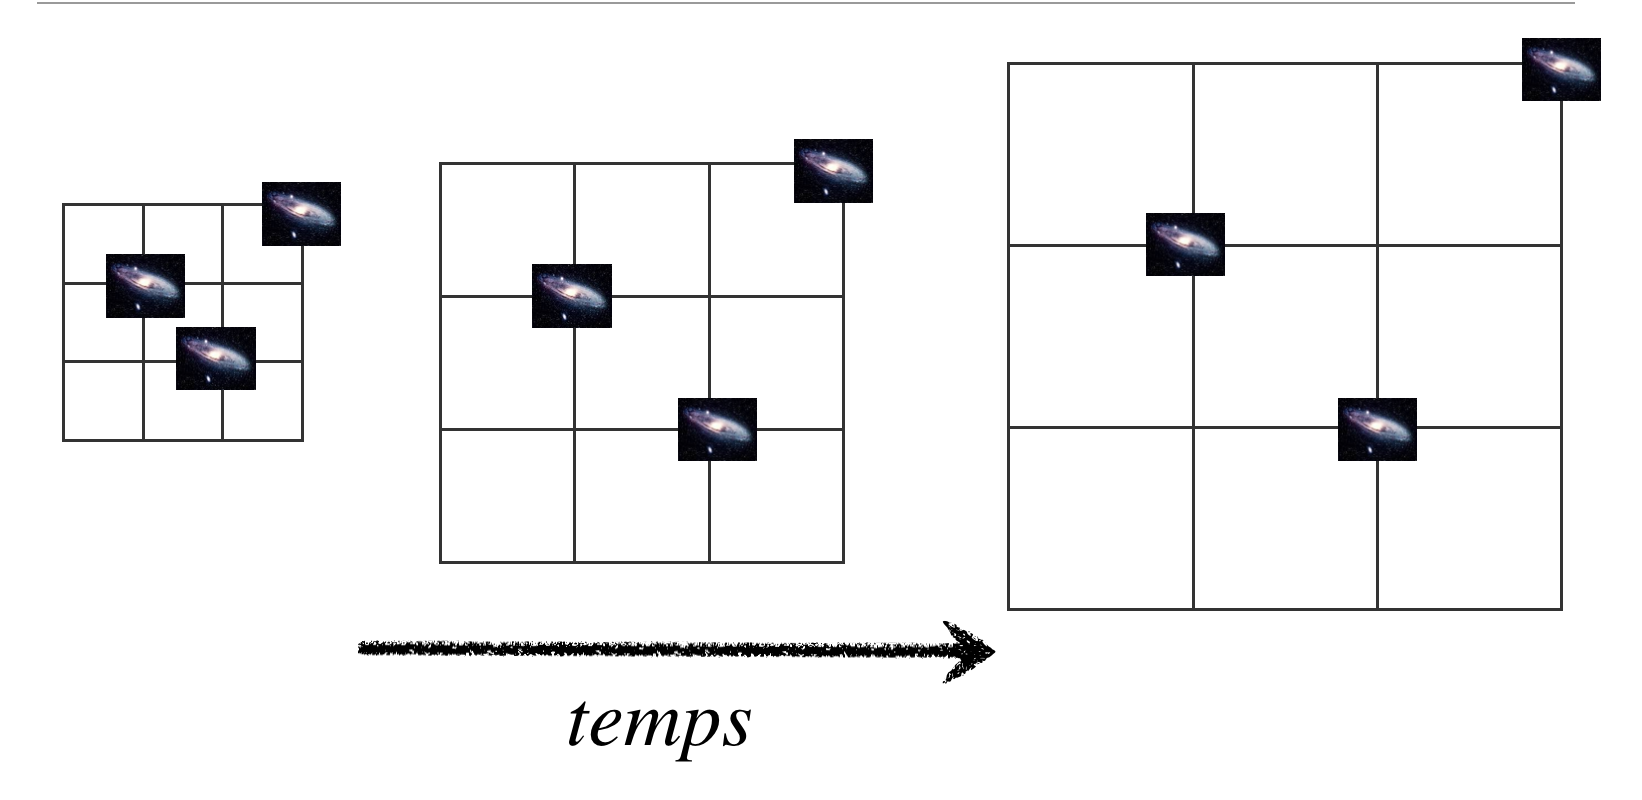
\includegraphics[height=10cm]{figs/grille.png}
	\caption[Coordonnées comobiles et expansion]{Une représentation schématique de la différence entre distance comobile et physique. Ces trois galaxies s'éloignent les unes des autres au cours du temps sous l'effet de l'expansion de l'Univers : l'espace se "dilate" comme indiqué par la grille dont les carreaux deviennent de plus en plus grands. La distance comobile est la distance mesurée en unités de carreaux : ces distances ne varient pas au cours du temps, car les galaxies sont immobiles par rapport à leur espace local. La distance physique, est la vraie distance mesurée avec une règle sur cette page : de façon évidente celle-ci varie pour toutes les paires de galaxies. Notons que ces distances physiques varient mais fondamentalement les galaxies sont toutes immobiles par rapport à l'espace sur lesquelles elles reposent.}
	\label{f:grille}
\end{figure}

\subsection{Facteur d'expansion, Loi de Hubble}
La distance physique $r(t)$ entre deux points peut être simplement dérivée au cours du temps.
\begin{equation}
\dot r(t)= \dot a S_K(r_0) =\frac{\dot a}{a}r(t).
\end{equation}
On définit la \textit{fonction de Hubble}\index{Hubble!fonction} comme la fonction dépendante du temps donnée par :
\begin{equation}
H(t)=\frac{\dot a}{a}.
\label{e:hubble}
\end{equation}
A l'aide de cette nouvelle fonction, le taux de variation des distances peut s'exprimer comme une fonction linéaire de la distance, \textit{la loi de Hubble}\index{Hubble!loi}
\begin{equation}
\dot r(t) = H(t) r(t).
\label{e:hubble2}
\end{equation}
Si $a$ est une fonction croissante, les distances physiques varient d'autant plus qu'elles sont importantes.

Plusieurs remarques peuvent être faites à propos des Eqs \ref{e:hubble} et \ref{e:hubble2}.  La première est que la fonction de Hubble n'est pas une constante temporelle, en revanche sa valeur ne dépend pas du point de l'espace considéré : on peut considérer que c'est une constante \textit{spatiale} de valeur donnée dans tout l'Univers à un instant donné. Suivant la convention générique en cosmologie, sa valeur actuelle est notée avec un indice 0 et vaut environ
\begin{equation}
H_0 \sim 70 \mathrm{km/s/Mpc}.
\end{equation}
Cette valeur est déterminée expérimentalement via par exemple la mesure conjointe des distances et des vitesses de fuites d'objets à grande distance. Cette mesure nécessite une connaissance de la luminosité\index{luminosité} intrinsèque de ces objets \sidenote{on parle aussi de chandelles standards} : par comparaison avec leur luminosité apparente, la distance peut être déduite tandis que la vitesse s'obtient à partir du décalage vers le rouge\index{redshift}. Un diagramme de Hubble\index{Hubble!diagramme} peut alors être construit pour obtenir la valeur de $H_0$ (voir Fig. \ref{f:hubblediag}).
\begin{figure}[htbp]
	\centering
		\includegraphics[height=10cm]{figs/hubble.png}
	\caption[Diagramme de Hubble]{Diagramme de Hubble représentant la vitesse de fuite de différentes sondes astrophysiques à partir des données de Freedman et al. (2000). La ligne trace la relation attendue pour une valeur $H_0=72$ km/s/Mpc tandis que chaque point représente un objet dont la distance et la fuite sont connues. Les objets considérés sont soit des supernovæ (points bleus) soit des galaxies (points orange, vert et rouge) dont les distances sont déterminées avec 3 techniques différentes. On note que les supernovæ permettent de sonder les distances les plus lointaines et sont donc les plus contraignantes pour la mesure du paramètre de Hubble. }
	\label{f:hubblediag}
\end{figure}

On peut constater au vu des unités employées et au vu de la structure de l'équation \ref{e:hubble}, que le paramètre de Hubble a la dimension de l'inverse d'un temps. On définit ainsi le temps de Hubble par $t_H=H^{-1}$~: on verra par la suite que ce temps de Hubble\index{Hubble!temps} est une bonne approximation de l'âge de l'Univers\index{age de l'Univers@âge de l'Univers}. 

La seconde remarque porte sur le caractère linéaire de l'équation \ref{e:hubble2}~: on peut montrer que cela permet de conserver le caractère isotrope et homogène des points de vue (cf. Fig. \ref{f:canard}), comme exigé par le principe cosmologique\index{principe cosmologique}. Si la loi avait été constante ($\dot r \sim r^0$) ou bien quadratique ($\dot r\sim r^2$), l'homogénéité aurait été perdue. 

La dernière remarque porte sur le fait que la loi donnée par l'Eq. \ref{e:hubble2} donne l'impression que des récessions supraluminiques\index{supraluminique} sont autorisées ($\dot r>c$)~: il s'avère que cela est exact, mais le taux de variation de distance calculé ici n'implique pas de déplacement par rapport à un référentiel local inertiel (qui lui serait limité par $c$)\sidenote{ et qui est le régime d'application de la relativité restreinte} mais se rapporte à une dilatation  même de l'espace~: dit rapidement, ceci n'est pas la vitesse d'un corps en déplacement. Par exemple, insistons sur le fait que cette dilatation ne permet pas de transmettre d'information\index{information}.

\begin{figure}[htbp]
	\centering
		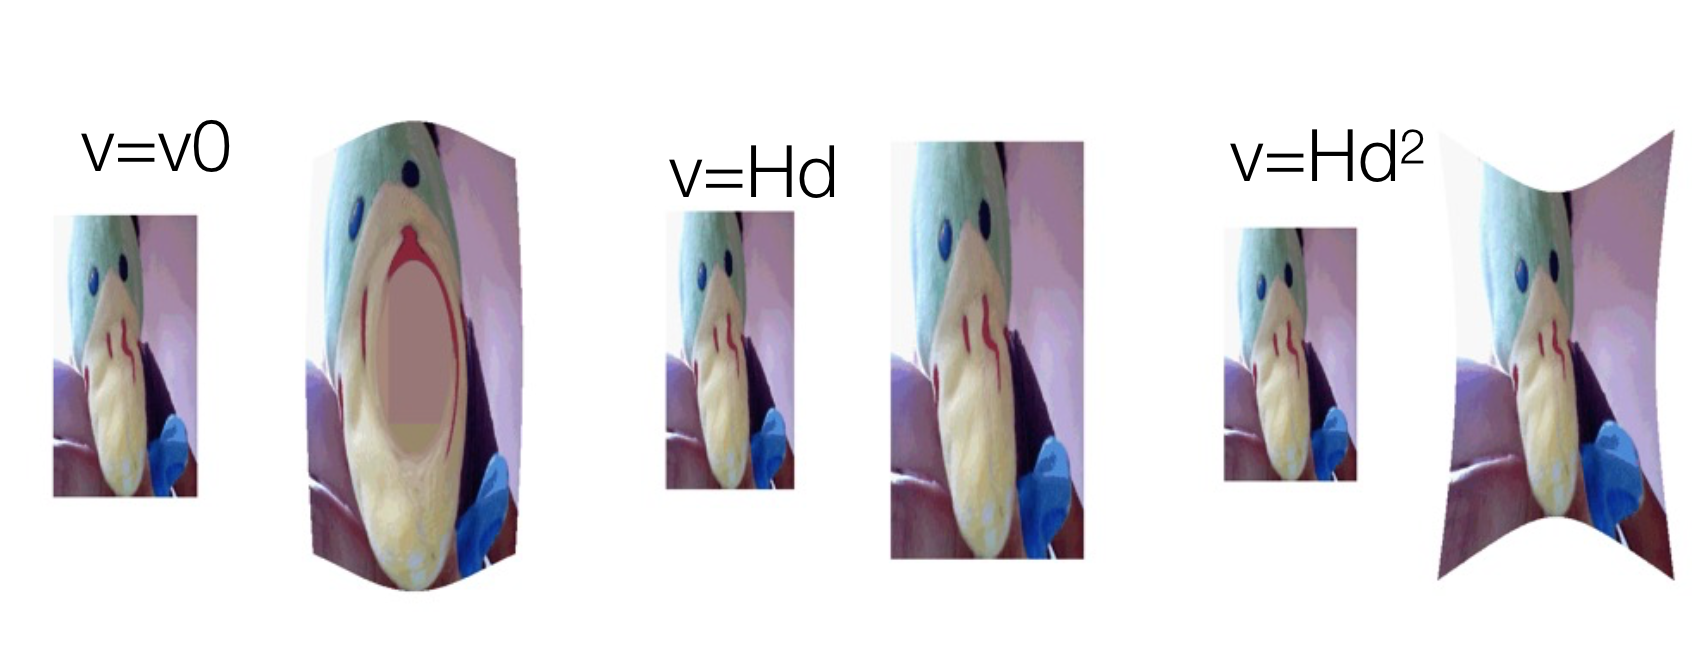
\includegraphics[height=6cm]{figs/canard.png}
	\caption[loi de Hubble et homogénéité]{La loi de Hubble établi une relation linéaire entre vitesse et distance physique. L'image du milieu montre comment une image est déformée par une telle loi linéaire, en fonction de la distance du pixel au centre de l'image : le canard devient plus grand mais n'est en pratique pas déformé. Les deux autres exemples montrent le même type de transformation mais en appliquant une déformation constante en fonction de la distance ou bien une déformation variant comme le carré de la distance. Dans ces 2 cas, le canard est déformé : si ce type de transformation avait été appliquée à un milieu homogène, cette dernière aurait été brisée. Par ailleurs, cette brisure dépendrait du choix de l'origine, en contradiction avec le principe d'homogénéité des points de vues.}
	\label{f:canard}
\end{figure}

\subsection{Décalage vers le rouge}
Nous venons de voir que la forme de la métrique FRW\index{Friedmann-Robertson-Walker!métrique} conduit naturellement à la Loi de Hubble. Dans le même ordre d'idée, la métrique FRW conduit naturellement à une modification de la perception des intervalles temporels. Si l'on considère par exemple l'émission d'un photon\index{photon} depuis un point E jusqu'à sa réception au point R, l'intervalle séparant les deux évènements est nul, $ds^2=0$, comme c'est toujours le cas pour une particule sans masse et se déplaçant à la vitesse de la lumière. Soit $E$ l'origine du système de référence, alors E et R se trouvent sur un seul et même rayon-vecteur ($d\theta=d\phi=0$) et FRW permet d'écrire:
\begin{equation}
\int_{t_E}^{t_R}c\frac{dt}{a(t)}=\int_{r_E}^{r_R}\frac{ dr_0}{\sqrt{1-Kr_0^2}}.
\end{equation}
Considérons un second photon qui va effectuer le même parcours mais en étant émis à l'instant $t_E+\delta_E$ et reçu à l'instant $t_R+\delta_R$. Dans un espace-temps statique, on s'attend à obtenir $\delta_E=\delta_R$. Pour ce second photon FRW permet d'écrire:
\begin{equation}
\int_{t_E+\delta_E}^{t_R+\delta_R}c\frac{dt}{a(t)}=\int_{r_E}^{r_R}\frac{ dr_0}{\sqrt{1-Kr_0^2}}.
\end{equation}
Notons que les bornes d'intégration du second membre restent inchangées, le second photon passant par les 2 même endroits en coordonnées comobiles: par conséquent les 2 intégrales temporelles des 2 photons sont identiques permettent d'écrire la relation :
\begin{equation}
\int_{t_E}^{t_E+\delta_E}c\frac{dt}{a(t)}=\int_{t_R}^{t_R+\delta_R}c\frac{dt}{a(t)}.
\end{equation}
Si l'on suppose que les délais temporels\index{délais temporels} $\delta_E$ et $\delta_R$ sont suffisamment petits par rapport au temps typique d'évolution du facteur d'expansion $a$, alors l'on obtient que le délai mesuré à la réception diffère du délai à l'émission:
\begin{equation}
\delta_R=\frac{a(t_R)}{a(t_E)} \delta_E.
\end{equation}
Cette relation est valable pour tous les délais~: si la métrique n'est pas statique $a(t_E)\neq a(t_R)$, les délais sont modifiés. Par exemple on constate que les courbes de lumières de supernovæ\index{supernovæ} sont affectées par cette modification des délais (voir Fig. \ref{f:wSN}). De même les flux\index{flux} de photons\sidenote{flux qui sont des nombres de photons reçus par intervalle de temps} subissent une "dilution" cosmologique à cause d'une modification de la durée s'écoulant entre 2 photons successifs. Enfin la \textit{longueur d'onde} $\lambda=cT$ est directement proportionnelle à une durée (la période). La longueur d'onde\index{longueur d'onde} d'un rayonnement électromagnétique reçu aujourd'hui est donc aussi affectée~:
\begin{equation}
\lambda_0=\frac{\lambda_E}{a(t_E)}
\end{equation}
où on a utilisé la convention $a(t_0)=1$. Il en découle que le décalage vers le rouge\index{redshift} est donné par
\begin{equation}
z = \frac{\lambda_0-\lambda_E}{\lambda_E}=\frac{1}{a_E}-1.
\end{equation}
Si le facteur d'expansion était plus petit dans le passé (comme attendu pour un Univers en expansion), le décalage vers le rouge (ou \textit{redshift}) est positif ou nul. Notons qu'à aucun moment il n'est fait mention de vitesse de déplacement de source ou de récepteur. Le seul effet est celui d'un espace-temps non-statique qui donne un effet similaire à un effet Doppler mais qui en aucun cas ne nécessite que la source ou l'émetteur possèdent une vitesse non-nulle par rapport à son référentiel localement inertiel.

\begin{figure}[htbp]
	\centering
		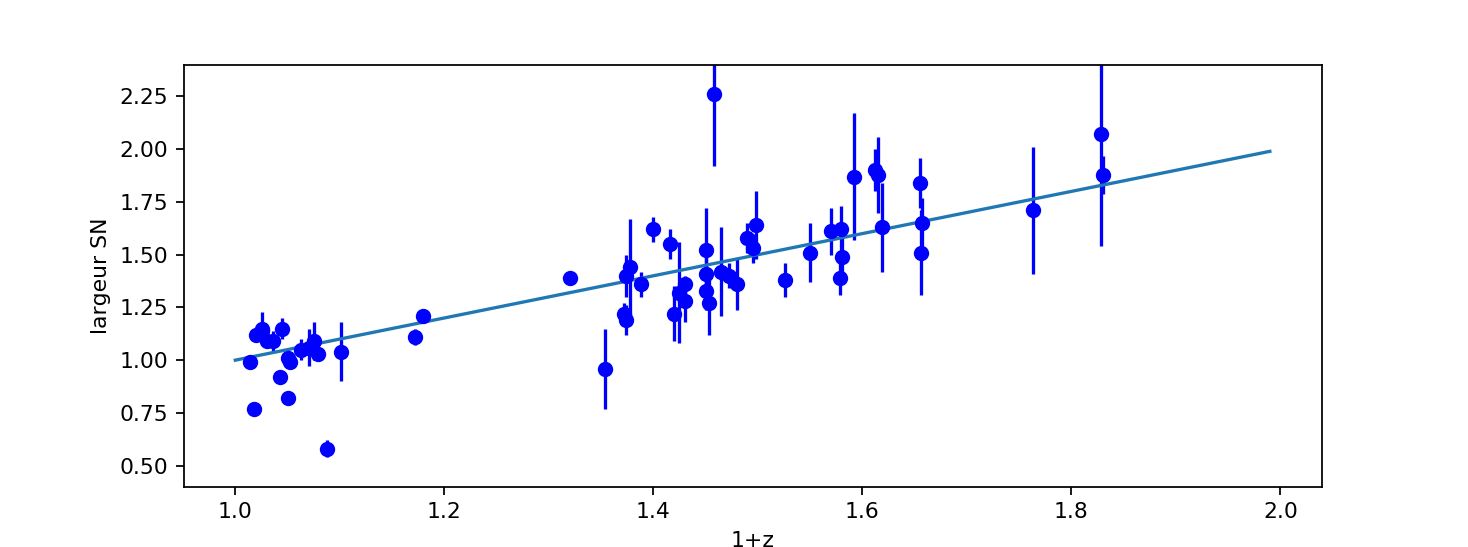
\includegraphics[height=6cm]{figs/wSN.png}
	\caption[Durée des supernovæ en fonction du redshift]{Un exemple de mesure des durées des supernovæ cosmologiques en fonction du redshift. Tous ces objets ont des courbes de lumières identiques car correspondant à l'explosion d'objets très similaires (des naines blanches d'environ 1.4 $M_\odot$). On constate que la durée des courbes de lumières associées varient en suivant une loi en $1+z$ où $z$ est le redshift : c'est l'effet cosmologique de dilatation des durées qui opère ici. Données issues de Goldhaber et al. 2001.}
	\label{f:wSN}
\end{figure}

\subsection{Source de la gravitation}
A ce stade, l'élément essentiel qui reste à préciser est la loi qui régit l'évolution du facteur d'expansion et par extension celle de la métrique FRW\index{Friedmann-Robertson-Walker!métrique}. Plus généralement quelles sont les lois qui permettent de relier la métrique $g_{\mu\nu}$ (donc la structure de l'espace-temps) aux sources de la gravitation ? Ces relations sont connues et portent le nom d'équations d'Einstein\index{equation d'Einstein@équation d'Einstein}. Leur détermination exacte est une démarche relativement complexe mais le cheminement logique qui aboutit à leur obtention peut être aisément décrit. 

Un bon point de départ est l'équation de champ de la gravitation Newtonienne, à savoir l'équation de Poisson\index{equation de Poisson@équation de Poisson}. Elle relie la densité de matière $\rho$ au potentiel gravitationnel\index{potentiel gravitationnel} $\phi(x)$, qui est une fonction simple du champ de gravitation~:
\begin{equation}
\Delta \phi =\rho.
\label{e:poisson}
\end{equation}
Clairement, le potentiel gravitationnel a pour source la densité de matière. En RG, l'objectif est d'obtenir une équation de champ analogue mais reliant $g_{\mu\nu}$ à ses sources. Disons d'emblée que dans le régime des champs faibles( dans lequel la gravitation Newtonienne s'applique) métrique et potentiel gravitationnel sont directement relié.

Quelles sont à priori les sources de la métrique en RG ? Une première tentative peut être effectuée en considérant directement la densité de matière \index{densité!matière}$\rho$ comme source~: c'est le cas quand les champs sont faibles et la matière est source de gravitation donc de géométrie. Toutefois on sait également que la masse en tant que telle ne joue pas de rôle central dans les théories relativistes, c'est davantage \textit{l'énergie}\index{energie@énergie} $E$ qui joue un rôle de premier plan. 

La \textit{densité} énergie serait-elle cette source ? Il est clair qu'elle doive jouer un rôle, par exemple au travers de la densité d'énergie de masse $\rho c^2$, ce qui reviendrait simplement à considérer la contrepartie énergie de la source de gravité Newtonienne. La difficulté de cette option réside dans le fait que l'énergie n'est pas directement une quantité fondamentale, y compris en relativité restreinte~: l'énergie n'est qu'une composante d'un concept plus vaste qui est l'énergie-impulsion \sidenote{par ailleurs la valeurs de l'énergie dépend du système de référence choisi, ce qui plaide en sa défaveur}. Par conséquent si l'énergie source la gravité en RG, c'est au travers de l'énergie-impulsion\index{energie@énergie!énergie-impulsion} et non seule. Plus précisément c'est au travers d'une \textit{densité} d'énergie-impulsion.

Si on note l'énergie impulsion $(P^0,P^1,P^2,P^3)$ où $P^0=E$ (en supposant $c=1$), on arrive à des expressions de densités de type:
\begin{equation}
\frac{dP^\mu}{dx^\alpha dx^\beta dx^\gamma}.
\end{equation}
Notons que $\alpha,\beta,\gamma$ désigne toutes les coordonnées disponibles, \textit{temps} compris. Bien sûr la densité d'énergie sus-mentionnée fait partie des sources:
\begin{equation}
\frac{dE}{dx dy dz},
\end{equation}
tandis que l'expression suivante est tout aussi légitime pour constituer un terme source de la gravité:
\begin{equation}
\frac{dP_x}{dtdydz}.
\end{equation}
Cette dernière expression désigne une force ($dP_x/dt$) divisée par une surface $dydz$ à $x$ constant\sidenote{c'est littéralement le flux de $P$ par unité de temps au travers de la surface $dydz$ perpendiculaire à $dx$}, à savoir une pression suivant la direction $x$\index{pression}. Notons qu'une pression est homogène à une densité d'énergie.

En généralisant cette expression, on obtient le tenseur des contraintes ou \textit{tenseur énergie-impulsion}
\begin{equation}
T^{\mu\delta} = \frac{dP_\mu}{dx^\alpha dx^\beta dx^\gamma}.
\end{equation}
obtenu en considérant la densité de la composante $\mu$ de $P$ sur la "surface" de coordonnées $x^\delta$ constante. C'est la source de la métrique, qui généralise la densité de masse du cas newtonien.  Comme mentionné ci-dessus, la densité d'énergie a donc un rôle à jouer mais également la pression, de même que le cisaillement \sidenote{qui est une force parallèle à une surface, complémentaire à la pression qui est perpendiculaire à une surface}. Par la suite la contribution d'un type d'énergie à la dynamique de l'espace-temps devra s'évaluer au vu de toutes ces quantités. 

Notons que $T$ obéit à une équation analogue à généralisation de la conservation de l'énergie\index{conservation de l'énergie} dans un espace-temps quelconque : 
 \begin{equation}
 \nabla_\nu T^{\mu\nu}=0,
 \label{e:divT}
 \end{equation}
 cette relation est tensorielle et non triviale et définit une "conservation" globale de l'objet $T$. La densité d'énergie est l'une des composantes de cet objet et n'est pas généralement conservé \textit{individuellement}, ne serait-ce que parce que l'expression de la densité d'énergie dépend du système de coordonnées choisi.

A ce stade, le terme source de la dynamique de l'espace-temps est connu, reste à expliciter l'opérateur différentiel qui agit sur la métrique et qui joue un rôle analogue au laplacien de l'équation \ref{e:poisson}. En d'autres termes quel est le tenseur $G$ , fonction de la métrique qui permette d'avoir:
\begin{equation}
G^{\mu\nu}=T^{\mu\nu}.
\end{equation}
Sans rentrer dans les détails, on cherchera à obtenir un opérateur différentiel du second ordre, tout comme pour l'équation de Poisson\index{equation de Poisson@équationde Poisson} newtonienne. De plus il faut que l'équation \ref{e:divT} soit satisfaite par $G$. L'opérateur différentiel du second ordre le plus simple permettant de satisfaire à cette contrainte est le \textit{tenseur d'Einstein}\index{tenseur d'Einstein}
\begin{equation}
G^{\mu\nu}=R^{\mu\nu}-\frac{R}{2}g^{\mu\nu}
\label{e:einstein}
\end{equation}
où $R^{\mu\nu}$ est le tenseur de Ricci\index{tenseur de Ricci} ou \textit{tenseur de courbure} et qui dépend de dérivées de second ordre de $g^{\mu\nu}$. $R$ est la trace de ce tenseur et est appelé aussi scalaire de courbure ou scalaire de Ricci.

Pour résumer, l'équation de champ de la gravité dans le cadre de la relativité générale décrit le comportement de la métrique en fonction du contenu local en énergie, via :
\begin{equation}
G^{\mu\nu}=T^{\mu\nu}.
\label{e:RG}
\end{equation}
Plusieurs remarques peuvent être faites à ce stade. La première est que nous sommes passé d'une équation scalaire dans le cas newtonien à une équation tensorielle avec dans l'absolu $ 4\times 4=16$ équations couplées à résoudre. Toutefois le tenseur d'énergie-impulsion\index{energie@énergie-impulsion} est symétrique et au final seules 10 équations restent réellement indépendantes dans le cas générique. De plus si les sources d'énergies possèdent un certain degré d'isotropie (comportement de fluide parfait\index{fluide parfait}\sidenote{c'est-à-dire un fluide sans viscosité ni cisaillement} par exemple) les composantes anisotropes de la pression ne rentrent pas en jeu et le système peut encore être réduit. La seconde remarque porte sur la structure du tenseur d'Einstein (Eq. \ref{e:einstein}). On constate ainsi que l'opérateur est non linéaire  en métrique (via par exemple $\frac{R}{2}g^{\mu\nu}$), ce qui rend l'équation de champ particulièrement complexe à résoudre dans le cas général. On constate également que la métrique $g^{\mu\nu}$ est elle-même source de courbure. Cela est particulièrement manifeste en écrivant l'équation \ref{e:RG} avec un terme supplémentaire:
\begin{equation}
G^{\mu\nu}=T^{\mu\nu}+\Lambda g^{\mu\nu}
\label{e:modifeins}
\end{equation}
où $\Lambda$ est un scalaire constant dans l'espace-temps. Compte tenu de $\nabla_\mu g^{\mu \nu}=0$, il en découle que l'équation \ref{e:modifeins} reste valable et dans ce cas  la métrique est également source de courbure. Notons que le scalaire $\Lambda$ introduit dans l'équation Eq. \ref{e:modifeins} s'interprète comme une \textit{constante cosmologique}\index{constante cosmologique}.

\section{Équations de Friedmann}
Comme indiqué dans la section précédente, l'hypothèse d'un Univers homogène et isotrope conduit à une forme de la métrique donnée par FRW\index{Friedmann-Robertson-Walker!métrique}. Considérant de plus que la relativité générale fournit une bonne description de la dynamique de l'espace temps, on est en principe capable de résoudre les équations d'Einstein pour une métrique FRW. Le résultat de cette opération est \textit{l'équation de Friedmann}. Elle repose sur la RG, sur la métrique de FRW et considère que le contenu en énergie de l'Univers est bien décrit par des "fluide" parfaits\index{fluide parfait}, de pression isotrope et sans viscosité.

L'équation de Friedmann\index{equation de Friedmann@équation de Friedmann} est une relation scalaire qui relie le facteur d'expansion $a(t)$, qui restait la dernière quantité non précisée de la métrique, au contenu en énergie de l'Univers~:
\begin{equation}
\frac{\ddot a}{a}=-\frac{4\pi G}{3c^2}(\rho c^2 +3 P),
\label{e:friedmann}
\end{equation}
où $\rho c^2$ est la densité d'énergie de l'Univers et $P$ sa pression, qui sont toutes deux fonctions du temps et donc de $a$. On constate que comme prévu, la dynamique de l'espace temps est lié à son contenu énergétique. Notons que \textit{à priori} le second terme est défini positif, donc la dynamique de l'Univers semble être décélérée $\ddot a<0$. Un modèle d'Univers se définira à partir d'une solution de cette équation différentielle, qui elle même dépendra du contenu en énergie. C'est l'objet du chapitre suivant.
%%!TEX root = /Users/domaubert/Documents/Lectures/cosmologie/cosmo_main.tex

\chapter{Dynamique de l'Univers Homogène}
Nous savons dorénavant que les distances $r$ entre deux points de l'Univers peuvent évoluer au cours du temps, suivant une simple loi d'échelle:
\begin{equation}
r(t)=a(t)r_0
\end{equation}
où $r_0$ désigne la distance actuelle entre 2 points. La facteur sans dimension $a(t)$ encode toute la dépendance temporelle de l'évolution des distances dans l'Univers homogène. Reste à présent à déterminer l'évolution temporelle de ce facteur $a(t)$, appelé aussi \textit{facteur} ou \textit{paramètre} d'expansion.
En particulier l'un des objectif est de parvenir à comprendre l'histoire observée de notre Univers avec un Big-Bang ($a\rightarrow 0$ quand $t\sim 0$), des distances qui augmentent avec le temps ($\dot a>0$) et une expansion récente accélérée ($\ddot a>0$ quand $t\sim t_0$).

\section{Fluides Cosmologiques}

\begin{figure}[htbp]
	\centering
		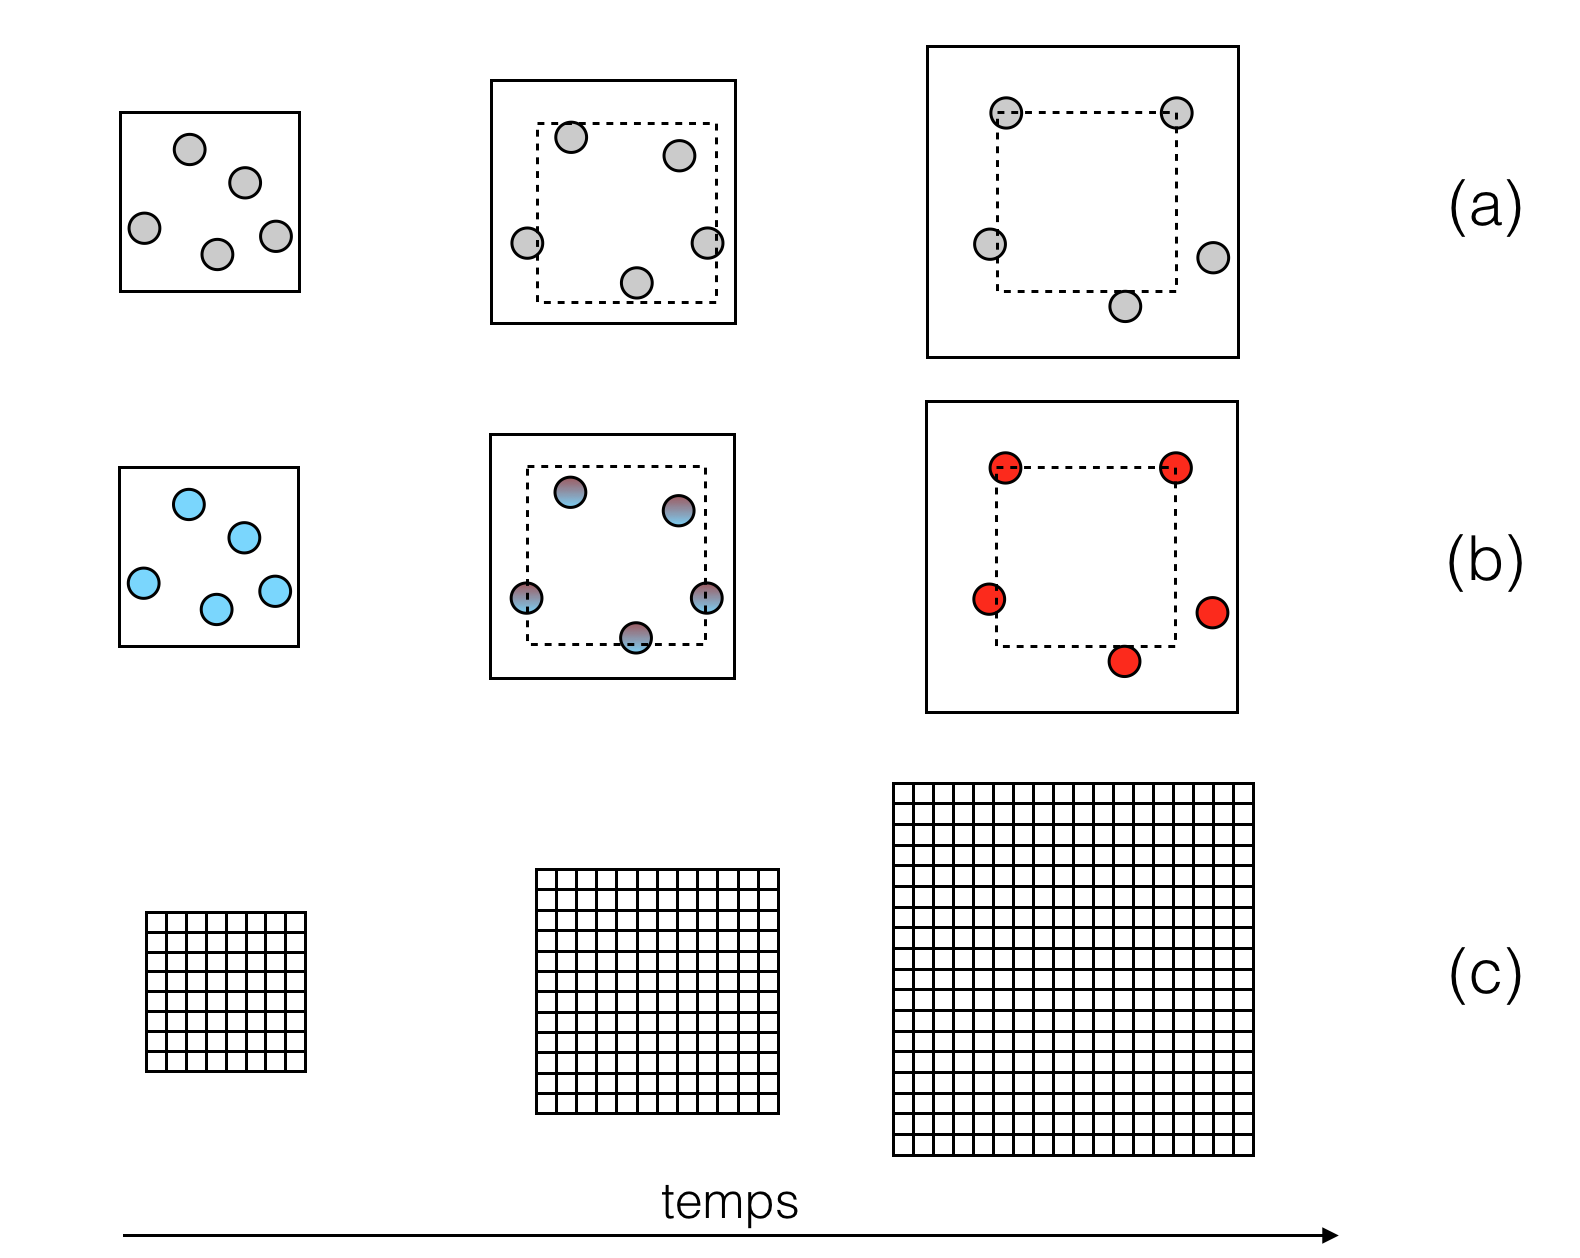
\includegraphics[height=10cm]{figs/fluides.png}
	\caption{Evolution schématique des 3 fluides cosmologiques sous l'effet de l'expansion. Pour la matière non-relativiste (a), le nombre de particules reste constant, l'énergie totale est constante et la densité d'énergie diminue avec le volume. Pour la matière relativiste (b), le nombre de particules reste constant mais l'énergie individuelle de chacune diminue sous l'effet du rougissement cosmologique: l'énergie totale diminue et la densité d'énergie diminue sous le double effet du rougissement et de la dilution. Pour le 'volume' (c), la densité d'énergie est constante dans chaque élément de volume (représenté par une case) et l'énergie totale à l'intérieur du volume de contrôle augmente avec l'expansion.}
	\label{f:fluides}
\end{figure}

On désigne par \textit{fluides} les différentes formes sous lesquelles l'énergie-impulsion se trouve stockée dans l'Univers. Ces fluides opèrent comme termes  sources de l'équation de Friedmann (Eq. \ref{e:friedmann}) et régissent donc la dynamique de l'espace-temps. 

Ces fluides sont supposés isotropes et parfaits (non visqueux): leur pression se résume donc à un scalaire comme pour un fluide "standard". Par la suite on distinguera 3 types de fluides cosmologiques:
\begin{itemize}
\item la \textit{matière} qui désigne plus précisément la matière non-relativiste et qui se distinguera par une pression négligeable,
\item le \textit{rayonnement} qui désigne par abus de langage toute forme de matière relativiste. Sa pression est non nulle,
\item le \textit{volume} qui désigne une forme d'énergie dont la densité volumique est constante. Comme expliqué par la suite, on parle aussi de \textit{vide}.
\end{itemize}
Ces 3 fluides cosmologiques sont définis par des densités d'énergie et des pressions dont les comportements diffèrent, notamment en fonction du paramètre d'expansion $a$. Par la suite, on pourra démontrer que leurs contributions à l'histoire de la dynamique de l'Univers vont se faire à différentes époques et suivant différentes dépendances temporelles.

Afin de comprendre leurs influences respectives sur la dynamique du cosmos, la procédure à suivre sera toujours plus ou moins identique. Rappelons l'expression de l'équation de Friedmann:
\begin{equation}
\frac{\ddot a}{a}=-\frac{4\pi G}{3c^2}(\rho c^2 +3 P).
\end{equation}
Nous voyons que la dépendance temporelle de $a(t)$ (décrite par le membre de gauche de l'équation) est 'sourcée' par les quantités du membre de droite qui caractérisent la matière contenue dans l'Univers.
Pour intégrer cette équation et trouver une expression pour $a(t)$, il s'agit donc de connaitre la densité d'énergie du fluide cosmologique ainsi que la pression qui l'accompagne: ces quantités constituent les \textit{sources} de la variation de $a$ et donc de la dynamique des distances dans l'Univers. 

Notons que dans le cas général, $\rho=\rho(t)=\rho(a)$ et $P=P(t)=P(a)$. Le terme source va donc varier au cours du temps (ou de façon équivalente en fonction de la valeur du facteur d'expansion), et va donc modifier le comportement de $a(t)$. Si jamais plusieurs fluides se trouvent être présents simultanément, chacun aura sa propre contribution au terme source de l'équation de Friedmann dont l'expression devient alors:
\begin{equation}
\frac{\ddot a}{a}=-\frac{4\pi G}{3c^2}\sum_i^\mathrm{fluides}(\rho_i c^2 +3 P_i).
\end{equation}

Généralement, la densité d'énergie $\rho_i c^2$ est facilement obtenue en faisant un bilan du nombre de particules du fluide considéré. Ici le fluide est considéré comme libre, non-soumis à une interaction extérieure, et chacun de ses éléments emmène une énergie:
\begin{equation}
E^2=p^2c^2+m^2c^4,
\end{equation}
constitué de son énergie cinétique et de son énergie de masse.

La pression nécessite généralement un peu plus d'effort. Afin d'évaluer cette pression, une approche consiste à considérer que la \textit{variation} d'énergie interne avec le volume est due au travail des forces de pression. Ainsi si on considère un volume de contrôle que l'on fait varier d'une quantité $dV$, la variation interne d'énergie est proportionnelle à cette pression:
\begin{equation}
dE=-PdV,
\label{e:therm1}
\end{equation}
il ne s'agit ni plus ni moins que d'une application du premier principe de la thermodynamique. En cosmologie, la source de variation du volume d'un contour est la dynamique de l'Univers, via le facteur d'expansion. Ainsi le volume $V$ mesuré à n'importe quel instant peut être exprimé en fonction du volume mesuré aujourd'hui, $V_0$, du même contour:
\begin{equation}
V=V_0a^3,
\end{equation}
d'où l'expression suivante pour la variation $dV$
\begin{equation}
dV=V_03a^2da=3V\frac{da}{a}.
\label{e:dV}
\end{equation}
Notons par exemple que le taux de variation du volume est donné par:
\begin{equation}
\frac{dV}{dt}=3HV
\end{equation}
et fait intervenir le paramètre de Hubble, $H(a)=\dot a/a$.

\subsection{La matière non-relativiste}
Le premier fluide considéré est la matière non-relativiste, celle qui nous est la plus familière. On y trouve les baryons et toute forme de matière noire froide. Cette matière se caractérise par une énergie par particule dominée par l'énergie de masse et une énergie cinétique négligeable devant cette dernière ($pc\ll mc^2$)~:
\begin{equation}
E\sim mc^2.
\end{equation}
Supposons un volume de contrôle $V$ à l'intérieur duquel se trouve $N$ particules non-relativistes (voir Fig. \ref{f:fluides} (a)). A l'intérieur, la densité d'énergie vaut:
\begin{equation}
\rho_m c^2=\frac{Nmc^2}{V}=\frac{Nmc^2}{a^3V_0}=\rho_{m0}c^2\frac{1}{a^3}.
\label{e:densm}
\end{equation}
Ici la masse d'une particule est supposée constante et le volume de contrôle contient toujours le même nombre de particules. Cette dernière hypothèse revient à considérer qu'il n'y a aucune création ou destruction nette de particules et que le flux net au travers de la surface délimitant ce volume est nul : pour un Univers homogène, donc sans variations spatiales susceptibles de générer des mouvements de matière, cette dernière hypothèse est raisonnable. L'équation \ref{e:densm} nous renseigne sur l'évolution temporelle de la densité d'énergie de la matière non-relativiste. Dans un Univers en expansion, $a$ est une fonction croissante du temps :  on constate alors que cette densité diminue au cours du temps, par simple dilution d'un nombre constant de particules (et donc d'énergie totale) dans un volume de plus en plus grand. Toujours dans le cas d'un facteur d'expansion croissant avec le temps, on constate que la densité d'un tel fluide était plus importante dans le passé.

Qu'en est-t-elle de la pression de ce fluide non relativiste ? Si l'on met à profit l'équation \ref{e:therm1}, on obtient:
\begin{equation}
P_m=-\frac{dE_m}{dV}
\end{equation}
où $E_m$ est l'énergie totale dans le volume de contrôle considéré. Dans le cas présent cette énergie est complètement dominée par l'énergie de masse, qui est constante dans ce volume, y compris lorsque le volume est modifié par la dynamique de l'Univers. Par conséquent, pour un fluide non-relativiste, la pression est considérée comme négligeable:
\begin{equation}
P_m=0.
\end{equation}
Ceci n'est pas une totale surprise: en effet nous avons défini ce fluide non-relativiste comme étant \textit{absolument froid}, i.e. avec une contribution nulle (en pratique négligeable) de l'énergie cinétique à son énergie interne totale. Pour mémoire, la pression est une manifestation des mouvements microscopiques des particules individuelles: celles-ci étant figées, il en résulte une pression égale à zéro.

\subsection{La Matière Relativiste}
On désigne par matière relativiste toute forme de matière pour laquelle la contribution de son énergie cinétique domine celle de son énergie de masse. Pour une particule de ce fluide, nous avons $mc^2\ll pc$ et son énergie individuelle est donnée par:
\begin{equation}
E\sim pc,
\end{equation}
où $p$ désigne l'impulsion de la particule. Cela concerne bien évidemment les photons mais également toute particule très légère comme les neutrinos. Supposons le même volume de contrôle que pour la matière non relativiste, avec une densité $N$ de particules chacune porteuse d'une énergie $pc$ (voir Fig. \ref{f:fluides} (b)). Comme précédemment, la densité d'énergie de ce volume de contrôle est donnée par:
\begin{equation}
\rho_rc^2=\frac{Npc}{V}.
\end{equation}
Toutefois, contrairement à la masse, l'impulsion est sensible à la dynamique de l'Univers puisqu'elle peut s'exprimer en fonction de la longueur d'onde qui elle-même subit les effets de rougissement cosmologique:
\begin{equation}
p=\frac{hc}{\lambda}=\frac{hc}{a\lambda_0}=\frac{p_0}{a}.
\end{equation}
Il en résulte une dépendance temporelle de la densité d'énergie relativiste qui est différente de celle trouvée précédemment pour la matière non-relativiste~:
\begin{equation}
\rho_rc^2=\frac{Np_0c}{ a^4 V_0}=\rho_{r0}c^2\frac{1}{a^4}.
\end{equation}
Comparée à la matière non-relativiste, la densité d'énergie varie ici plus rapidement (et baisse plus rapidement si $a$ croît avec le temps). La raison est simple~: en plus de l'effet de dilution géométrique s'ajoute une baisse de l'énergie individuelle portée par chaque particule à cause du rougissement cosmologique.

Calculons maintenant la pression comme taux de variation de l'énergie totale avec le volume:
\begin{equation}
P_r=\frac{dE_r}{dV}=-\frac{d(Npc)}{dV}.
\end{equation}
Grâce à l'équation \ref{e:dV} la pression peut être réexprimée en fonction de la densité d'énergie:
\begin{equation}
P_r=Nc\frac{d(p)}{dV}=Nc\frac{dp}{da}\frac{da}{dV}=-Nc\frac{-p_0}{a^2}\frac{a}{3V}=\frac{1}{3}\rho_rc^2.
\end{equation}
Dans ce cas la pression est non nulle et est une fonction simple de la densité d'énergie. A nouveau cela n'est pas une surprise puisque nous avons défini ces particules comme ne possédant qu'une énergie cinétique, qui est la source de pression.

\subsection{Le "Volume"}
De prime abord, le dernier type de fluide est de nature hypothétique et est \textit{défini} par une densité d'énergie constante:
\begin{equation}
\frac{dE_v}{dV}=\Lambda=\mathrm{const.}
\end{equation}
On appellera ce fluide "volume" car il ne repose pas sur l'existence d'une particule le composant mais davantage sur une quantité d'énergie qu'apporte nécessairement un volume donné. Remarquons que si le volume de contrôle augmente (sous l'effet d'un facteur d'expansion croissant par exemple), la quantité d'énergie présente dans ce volume de contrôle augmente aussi (voir Fig. \ref{f:fluides} (c)).  On parle aussi d'énergie du "vide", puisqu'une telle énergie est présente y compris en l'absence de matière.

Compte tenu de cette définition, la densité d'énergie vaut:
\begin{equation}
\rho_vc^2=\rho_{v0}c^2,
\end{equation}
tandis que la pression vaut
\begin{equation}
P_v=-\rho_vc^2.
\end{equation}
On constate qu'un tel type de contribution énergétique produit une pression \textit{négative}. A l'inverse du comportement d'un fluide standard, son énergie interne augmente avec son volume, le 'vide' ne subit pas de détente. Cela résulte de la non-variation de la densité d'énergie à l'intérieur du volume de contrôle même si celui-ci évolue sous l'effet du facteur d'expansion.

A nouveau ce fluide est une hypothèse de travail. Toutefois il s'avère que ce type de fluide exotique permet une bonne représentation de la dynamique \textit{observée} des distances dans l'Univers. Ce fluide est la fameuse \textit{énergie noire}, dont la nature nous échappe complètement actuellement et qui permet de rendre compte de l'accélération observée de l'expansion de l'Univers. La densité d'énergie étant constante dans le temps et dans l'espace, on parle aussi de \textit{constante cosmologique}.

\section{Epoques de domination}
\begin{figure}[htbp]
	\centering
		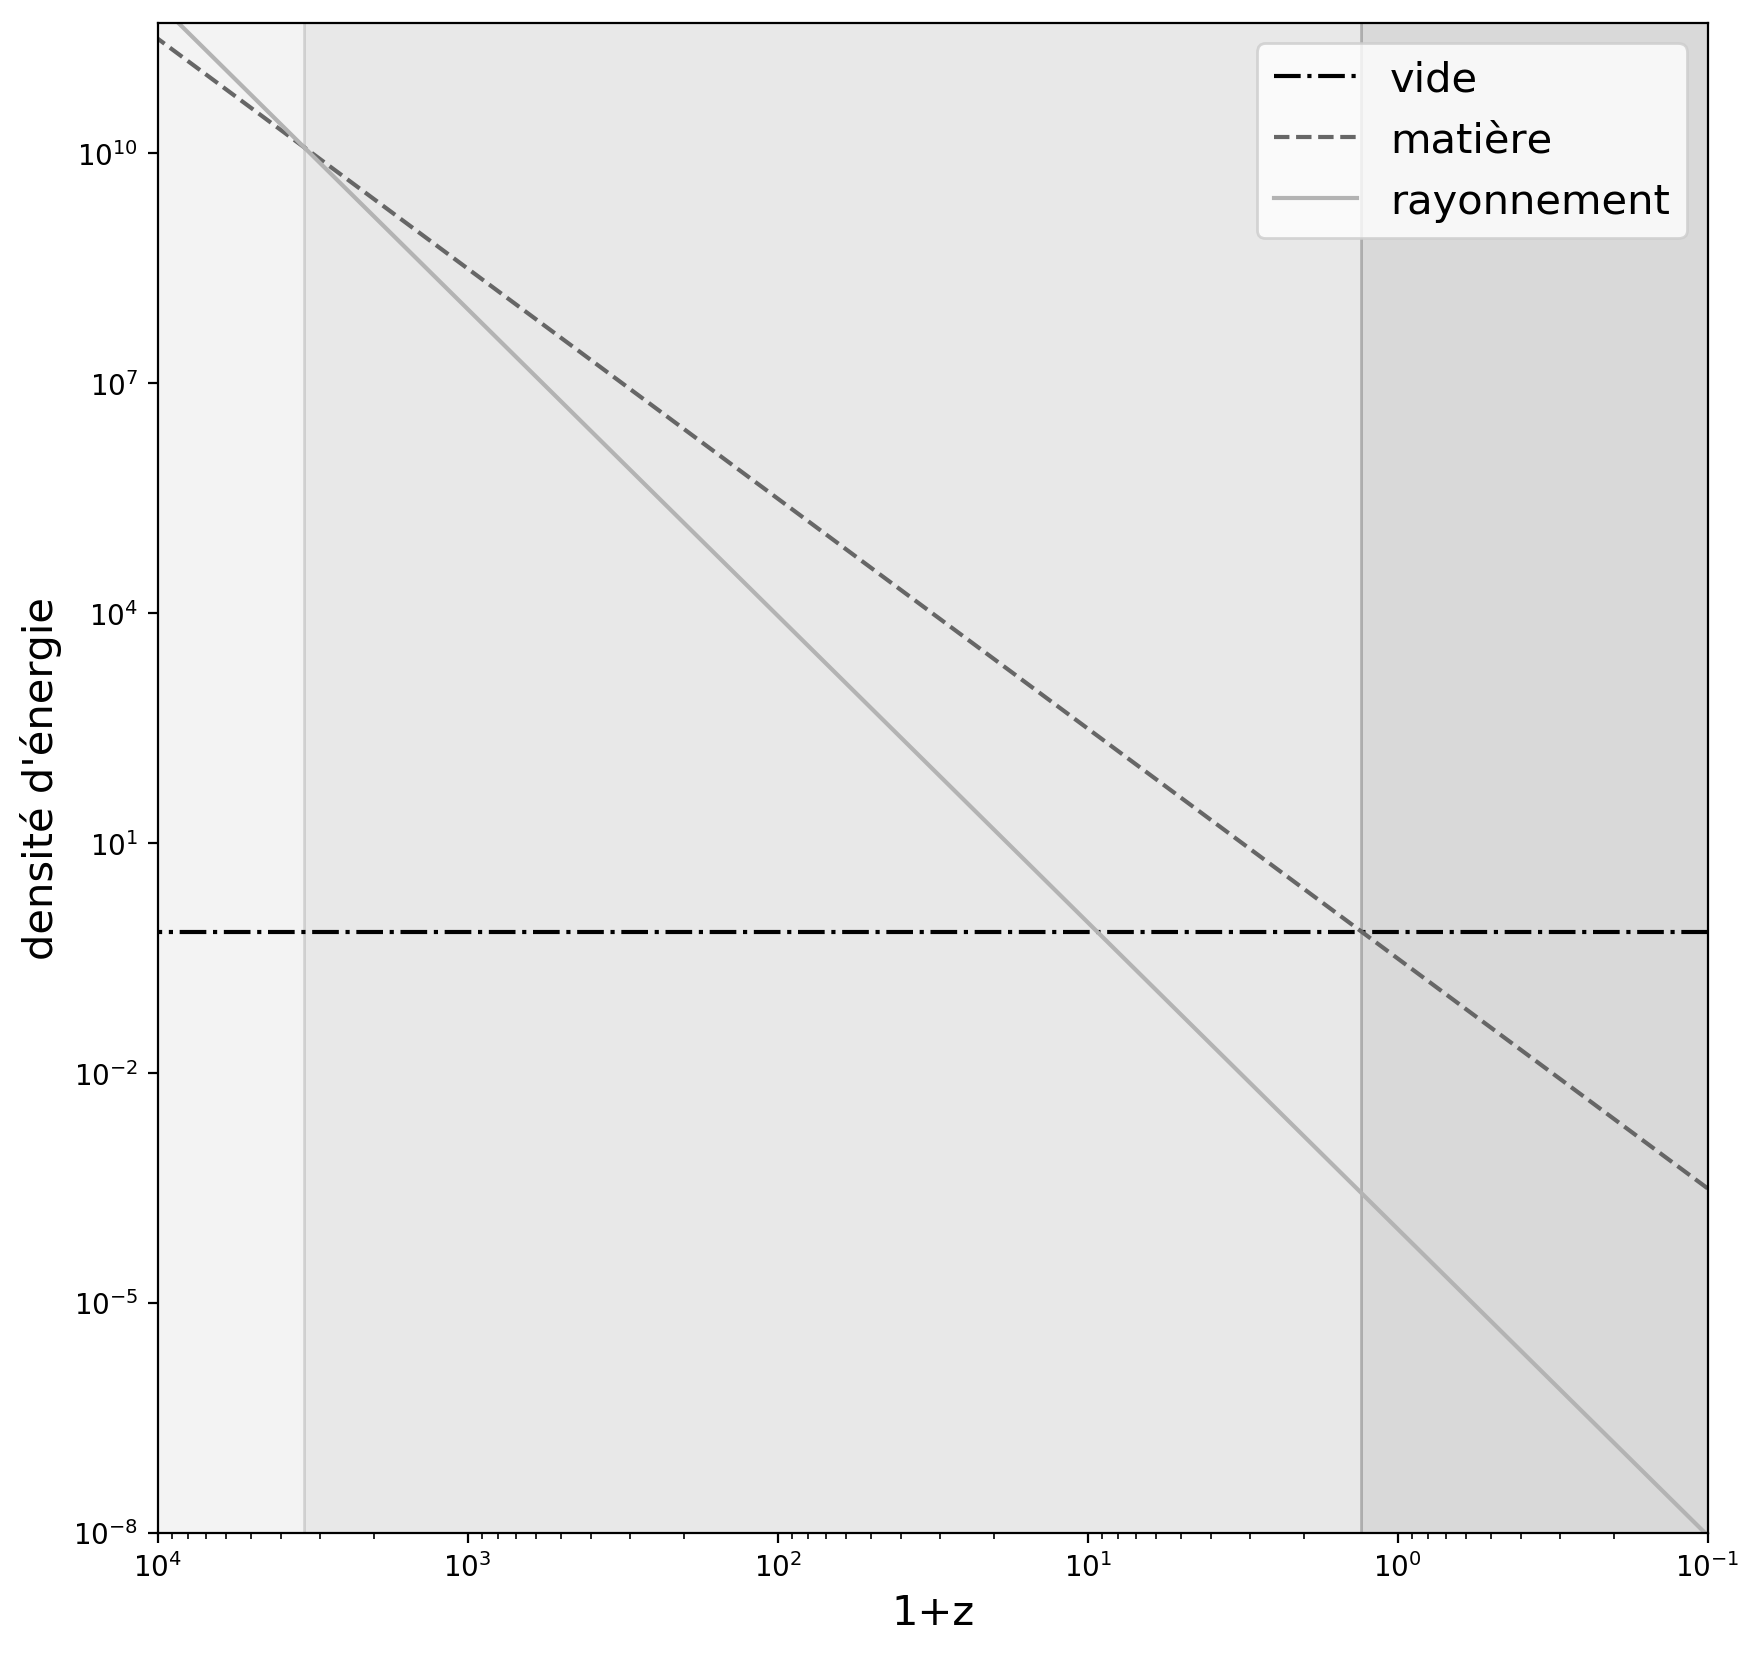
\includegraphics[height=10cm]{figs/era.png}
	\caption{Evolution temporelle de la densité d'énergie des 3 fluides cosmologiques pour une cosmologie standard. Le temps s'écoule de la droite vers la gauche, avec une domination successive du rayonnement, de la matière et du vide.}
	\label{f:era}
\end{figure}
Le bilan des trois fluides étudiés est donné dans la table suivante. On notera qu'on utilise la nomenclature standard des trois fluides: "matière" pour la matière non relativiste, "rayonnement" pour la matière relativiste et "vide" pour l'énergie de volume.
\begin{table}[h]
\begin{center}
\begin{tabular}{|c|c|c|c|}
\hline 
 & Caractéristique & Densité d'énergie & Pression \\ 
\hline 
Matière & $E\sim mc^2$ & $\rho_mc^2 =a^{-3}\rho_{m0}c^2$& $P_m=0$\\ 
\hline 
Rayonnement & $E\sim pc$ & $\rho_rc^2 =a^{-4}\rho_{r0}c^2$ & $P_r=\rho_rc^2/3$ \\ 
\hline 
Vide & $dE/dV\sim \mathrm{cst}$ & $\rho_vc^2 =\rho_{v0}c^2$ & $P_v=-\rho_vc^2$ \\ 
\hline 
\end{tabular} 
\end{center}
\caption{Les 3 fluides cosmologiques}
\end{table}

En réinjectant ces résultats dans l'équation de Friedmann (eq. \ref{e:friedmann})  on obtient une expression détaillée du terme source qui permet déjà d'entrevoir certaines caractéristiques de la dynamique des distances dans l'Univers:
\begin{equation}
\frac{\ddot a}{a}=-\frac{4\pi G}{3}(\frac{\rho_{m0}}{a^3}+2\frac{\rho_{r0}}{a^4}-2\rho_{v0}).
\label{e:esource}
\end{equation}
Dans un premier temps, il apparaît que la matière et le rayonnement ont un même effet qualitatif et tendent à décélérer la variation du facteur d'expansion (en imposant $\ddot a<0$). Cette décélération est d'autant plus faible que les distances  sont grandes (i.e. $\ddot a \rightarrow 0$ quand $a$ augmente) et que les densités d'énergies associées sont faibles, permettant d'anticiper sur une sorte de "régulation". A l'inverse, le "vide" produit une accélération de la variation de $a$ (avec $\ddot a>0$)~: cela résulte du terme de pression négative qui produit une contribution nette positive de ce fluide au terme source de l'équation de Friedmann. Notons que cette contribution reste constante au cours du temps, avec $\ddot a$ augmentant avec $a$, indiquant dès à présent un effet "catastrophique" non régulé. 

Enfin on constate que les contributions au terme source de l'équation de Friedmann ont des dépendances temporelles différentes en fonction du fluide considéré (voir Fig. \ref{f:era}). En supposant une évolution de $a$ croissante au cours du temps, il apparaît qu'entre le rayonnement (qui varie en $a^{-4}=(1+z)^4$) et la matière (qui varie en $a^{-3}=(1+z)^3$), la première domine aux époques correspondants aux faibles valeurs de $a$ (donc généralement au début) tandis que la matière doit prendre le dessus aux plus grandes valeurs du facteur d'expansion (donc généralement plus tard). Il existe donc une époque où ces deux fluides ont exactement la même densité d'énergie~: cette époque est appelée \textit{l'époque d'équivalence}. Avant, la matière relativiste domine, après la matière non-relativiste dicte la dynamique de l'Univers.

Mais qu'en est-il de la densité d'énergie du vide, dont la valeur est par définition constante? Le verdict est sans appel: compte tenu du fait que les densités d'énergie des deux autres fluides sont des fonctions décroissantes de $a$, il existe \textit{toujours} une valeur seuil du paramètre d'expansion au delà de laquelle le vide domine. Tout modèle d'Univers avec une énergie du vide finira par être dominé par cette dernière, pour peu que l'on attende suffisamment longtemps.

Pour finir, disons clairement que les relations obtenues entérinent la non-conservation de l'énergie totale du Cosmos. Pour un Univers dominé par une énergie du vide de densité d'énergie constante, l'expansion implique nécessairement des volumes croissants et donc une énergie totale croissante.  Même en l'absence de ce fluide inconnu, le rougissement individuel des photons fait que l'énergie totale stockée dans la matière relativiste doit décroître : la densité d'énergie varie en $a^{-4}$ et le volume en $a^3$ conduisant à une énergie totale non constante, inversement proportionnelle à $a$. Seul un Univers contenant uniquement de la matière non-relativiste, par conservation du nombre de particules d'énergie constante, garantit à priori une conservation de l'énergie totale : cet Univers n'est toutefois pas le nôtre qui contient à minima du rayonnement en plus de cette matière. Rappelons que cette non-conservation n'est pas problématique : la relativité générale ne garantit pas de façon générale la conservation du scalaire 'énergie' mais propose une relation plus complexe, plus générale sur le \textit{tenseur} énergie-impulsion. Par ailleurs, on peut se souvenir que la conservation de l'énergie est une traduction de l'invariance par translation temporelle du résultat d'une expérience donnée\footnote{de même que l'invariance par translation spatiale implique une conservation de l'impulsion ou l'invariance par rotation implique une conservation du moment cinétique} : dans un Univers où la géométrie possède une évolution, cette invariance n'est bien sûr pas garantie.

\subsection{Paramètre de densité $\Omega$}

A ce stade il nous faut introduire une nouvelle expression, le paramètre de densité $\Omega$, qui apparaît naturellement lorsque l'on intègre l'équation \ref{e:esource}. Cette intégration se fait naturellement en multipliant l'équation \ref{e:esource} par $2\dot a a$, qui permet d'obtenir:
\begin{equation}
\left(\frac{\dot a}{a}\right)^2=H(a)^2=\frac{8\pi G}{3}(\frac{\rho_{m0}}{a^3}+\frac{\rho_{r0}}{a^4}+\rho_{v0}-\frac{k}{a^2}).
\end{equation}
Notez l'introduction d'une constante d'intégration $k$ que nous discuterons par la suite. Le terme de gauche n'est autre que le carré du paramètre de Hubble au cours du temps: aussi pour des raisons de symétrie, il est tentant de multiplier le terme de droite par $H_0$, ce qui permet d'écrire:
\begin{equation}
H^2=H_0^2(\frac{\Omega_m}{a^3}+\frac{\Omega_r}{a^4}+\Omega_v-\frac{\Omega_k}{a^2}).
\label{e:hubblea}
\end{equation}
C'est cette équation qu'il faudra intégrer par la suite pour obtenir l'évolution temporelle du facteur d'échelle $a$ et elle introduit les paramètre de densités (dans l'ordre) de la matière, du rayonnement, du vide et de la constante d'intégration. Ces quantités sont sans dimension et égales à:
\begin{equation}
\Omega=\frac{\rho_0 c^2}{\rho_c c^2},
\end{equation}
où $\rho_c$ désigne la \textit{densité critique} dont l'expression est donnée par:
\begin{equation}
\rho_c=\frac{3H_0^2}{8\pi G}.
\end{equation}
Les paramètres de densités sont donc l'expression des densité d'énergie \textit{mesurées aujourd'hui} des différents fluides en unités de cette densité critique.

Si l'on applique l'équation \ref{e:hubblea} aujourd'hui quand $a=a_0=1$ on obtient une contrainte que doivent satisfaire tous les paramètres de densité, à savoir:
\begin{equation}
\Omega_m+\Omega_r+\Omega_v= 1+\Omega_k.
\end{equation}
Que représente $\Omega_k$ ? Si l'on remonte à l'expression des équations d'Einstein qui ont servi à produire l'équation de Friedmann, ce terme apparaît comme une courbure constante intrinsèque et est lié au coefficient de courbure $K$ de la métrique FRW (eq. \ref{e:FRW}). Si $\Omega_k>0$, donc $\Omega_m+\Omega_r+\Omega_v>1$ alors cela équivaut à une courbure positive donc sphérique. A l'inverse $\Omega_m+\Omega_r+\Omega_v<1$ produit une courbure négative de type hyperbolique. Enfin, $\Omega_k=0$  (correspondant à $\Omega_m+\Omega_r+\Omega_v=1$) est la marque d'une géométrie plane. 

Il est a noter qu'une simple inspection de la contribution de $\Omega_k$ au terme source de l'équation $\ref{e:hubblea}$ nous renseigne sur sa nature. En effet, on peut constater que les dépendances en $a$ de tous les paramètres en densité sont liés aux dépendances des densités d'énergies associées~: la matière est en $a^{-3}$ (densité d'énergie inversement proportionnelle au volume), le rayonnement en $a^{-4}$ (densité d'énergie inversement proportionnelle au volume + effet de rougissement) et le vide en $a^0$ (densité d'énergie constante en temps et en espace). Pour $\Omega_k$, on constate une dépendance en $a^{-2}$ comme le serait celle d'une courbure qui a bien la dimension du carré de l'inverse d'une longueur.

\subsection{Valeurs expérimentales des paramètres de densité}
Il existe plusieurs manières de déterminer ces quantités par l'observation, dont le détail sera donné par ailleurs. On peut toutefois donner dès à présent les valeurs standards de ces paramètres. 

Dans un premier temps, on constate que l'Univers possède une géométrie de courbure nulle. De même la contribution actuelle des espèces relativistes est proche de zéro. Enfin, on constate actuellement que l'Univers est en expansion ($\dot a>0$) et en accélération ($\ddot a>0$) ce qui indique une contribution significative de la densité d'énergie du vide. Au bilan voici qualitativement la répartition des différentes sortes d'énergie aujourd'hui:
\begin{itemize}
\item $\Omega_k<0.001$,
\item $\Omega_r\sim0.0001$,
\item $\Omega_m\sim 0.31$,
\item $\Omega_v\sim 0.69$.
\end{itemize}
On peut ajouter à ses paramètres la valeur actuelle du paramètre de Hubble $H_0=67$ km/s/Mpc et du paramètre de densité des baryons $\Omega_b\sim 0.049$.  Il en résulte un paramètre de densité pour la matière non baryonique de l'ordre de $\Omega_c=\Omega_m-\Omega_b\sim0.27$. Avec ce jeu de paramètres, le temps nous séparant du Big Bang (à savoir l'âge de l'Univers) est $t(a=1)=t_0\sim13.8$ milliards d'années. 

On constate que nous vivons actuellement dans un Univers dominé par l'énergie du vide. L'équivalence entre matière et rayonnement se produit pour $1+z_e=\Omega_m/\Omega_r$ et donne 
\begin{equation}
z_e\sim 3100
\end{equation}
correspondant à un Univers âgé de $t_e\sim 60 600$ ans. De même l'Univers a commencé à être dominé par le vide quand $1+z_\Lambda=(\Omega_v/\Omega_m)^{1/3}$ et donne
\begin{equation}
z_\Lambda\sim 0.3
\end{equation}
correspondant à un Univers âgé de $t_\Lambda\sim 10.2$ milliards d'années. 

Si l'on rassemble tous ces résultats, on observe que l'Univers est passé par 3 phases successives de domination de chacun des 3 fluides (voir aussi Fig. \ref{f:era}). Dans un premier temps, le bilan énergétique de l'Univers est dominé par le \textit{rayonnement}, au cours des 60 000 premières années. Puis c'est la \textit{matière} qui va  être le contributeur majeur de la dynamique de l'Univers pendant quelques milliards d'années. Enfin \textit{le vide} devient le fluide dominant, ce qui est toujours le cas aujourd'hui et dont la primauté ne fera que s'accentuer dans le futur.

\section{Modèles d'Univers}
Nous sommes à présent armés pour étudier des modèles simples d'Univers. L'équation maîtresse de ce type d'étude est l'équation \ref{e:hubblea} et l'objectif est d'obtenir l'expression de $a(t)$, la dépendance temporelle du facteur d'expansion. En toute généralité, cela nécessite de connaître les paramètres de densités et la solution ne peut être obtenue que par intégration numérique. Il existe toutefois toute une classe de modèles simples qui peuvent être résolus analytiquement et qui fournissent un bon aperçu du comportement quantitatif de la dynamique de l'Univers dans des cas plus généraux.

\subsection{Modèle d'Einstein-de Sitter : $\Omega_m=1$}
Ce modèle a une grande importance historique car il fut longtemps privilégié du fait de son caractère naturel. Le modèle \textit{Einstein-de Sitter}, appelé aussi \textit{Univers poussière}, considère un Univers plat et composé uniquement de matière, $\Omega_m=1$.  L'équation \ref{e:hubblea} devient alors simplement:
\begin{equation}
H(a)=\frac{\dot a}{a}=\frac{H_0}{a^{3/2 }}.
\end{equation}
Elle s'intègre facilement pour donner:
\begin{equation}
a(t)=\left(\frac{3H_0t}{2}\right)^{2/3}.
\end{equation}
ou bien
\begin{equation}
t=\frac{2}{3H_0}a^{3/2}.
\end{equation}
L'équation horaire du facteur d'expansion donne une loi de puissance "faible", décélérée comme attendue. Ce modèle inclut également un Big-Bang :
\begin{equation}
\lim_{t \to 0} a(t)=0
\end{equation}
impliquant des distances faibles et donc un Univers dense aux premiers instants.

L'âge de l'Univers peut également être déterminé en posant simplement $a=1$:
\begin{equation}
t_0=\frac{2}{3H_0}.
\end{equation}
On constate que le temps de Hubble mesuré aujourd'hui $t_H=H_0^{-1}$ est à peu de chose près l'âge de l'Univers. Prenant $H_0=67$ km/s/Mpc on obtient alors un âge d'Univers proche de 9.6 milliards d'années, bien en dessous de l'âge estimé de certaines étoiles par exemple ou de certains amas globulaires.  Bien que naturel, ce modèle ne permet pas d'expliquer l'âge observé de l'Univers. 

Une option longtemps envisagée fut de considérer une Univers à géométrie hyperbolique avec $\Omega_m<1$ auquel cas l'âge de l'Univers devient:
\begin{equation}
t_0=\frac{2}{3H_0\sqrt{\Omega_m}}.
\end{equation}
Pour $\Omega_m\sim0.3$ comme observé, on obtient un âge d'Univers compatible avec les plus vieux objets astronomiques, mais au prix d'une géométrie non plane. De plus il ne permet pas de produire une accélération de l'expansion, telle qu'observée aujourd'hui.

\subsection{Univers-Lumière, $\Omega_r=1$}
Dans ce cas, le contenu énergétique de l'Univers est dominé par le rayonnement et nous savons que ce n'est pas le cas aujourd'hui. Toutefois toute la physique de l'Univers primordial ($t<3$ minutes) se fait dans un régime où les espèces relativistes sont dominantes, comme dans ce modèle d'Univers-Lumière. Le principe est le même que précédemment où le paramètre de Hubble est donné par 
\begin{equation}
H(a)=\frac{\dot a}{a}=\frac{H_0}{a^2},
\end{equation} 
qui donne après intégration
\begin{equation}
a(t)\sim\sqrt{t}.
\end{equation}
Comme pour l'Univers poussière, ce modèle prédit un Big-Bang. L'expansion y est également décélérée avec toutefois une loi de puissance légèrement moins forte pour la variation temporelle du facteur d'expansion $a(t)$ (puissance $1/2$ au lieu de $2/3$). Cette différence trouve son origine dans une dilution plus rapide du terme source associé au rayonnement, avec une décroissance en $a^{-4}$ au lieu de $a^{-3}$.

\subsection{Univers de Sitter, $\Omega_v=1$}
Cet Univers est dominé par le vide avec une densité d'énergie constante et $\Omega_v=1$. Comme l'Univers lumière, ce modèle dit de \textit{de Sitter} ne peut être une représentation fidèle du cosmos observé mais il peut nous permettre d'avoir une vue qualitative de la dernière phase de la dynamique de l'Univers, régie par l'énergie du vide. Dans ce modèle, l'intégration de l'équation \ref{e:hubblea} donne 
\begin{equation}
t=H_0^{-1}\int_\epsilon^a\frac{da}{a},
\end{equation}
où l'on ne peut intégrer que depuis un temps arbitrairement faible mais non nul $\epsilon$ et ceci pour garantir la convergence de l'intégrale. La résolution de cette équation donne une loi d'expansion \textit{exponentielle}
\begin{equation}
a(t)=\epsilon e^{H_0 t}.
\end{equation}
Contrairement au deux modèles précédents, un tel Univers ne permet pas d'atteindre des distances arbitrairement faibles aux premiers instants et ne prédit pas de Big-Bang. Notons également que le paramètre de Hubble ne varie pas au cours du temps dans ce modèle:
\begin{equation}
H(t)=\frac{\dot a}{a}=H_0.
\end{equation}

Clairement, l'expansion est accélérée et est liée à l'absence de "dilution" de la densité d'énergie associée au vide~: bien qu'il y ait expansion, cela ne conduit pas à une diminution du terme source de l'équation de Friedmann. L'expansion ne peut être tempérée sous forme de loi de puissance douce et produit une dépendance exponentielle du facteur d'échelle. 

Pour finir, il faut mentionner que les théories de l'inflation suggèrent une histoire d'expansion primordiale (pour un Univers plus jeune que $10^{-34}$ seconde) de même nature, avec une évolution exponentielle de $a(t)$.  Comme expliqué dans le chapitre dédié à la période d'Inflation, cela suggère l'existence d'un champ (pour l'instant inconnu) dont le potentiel varie lentement (et donc une densité d'énergie quasi-constante) et à même d'entretenir cette expansion exponentielle.

\subsection{Cas général, modèle standard $\Lambda$CDM}
Dans une cosmologie arbitraire, l'évolution du facteur d'échelle ne peut être obtenue qu'en intégrant numériquement l'équation \ref{e:hubblea}, mais cette tâche ne présente aucune difficulté particulière avec les bons outils. 

La figure \ref{f:aexpcosmo} présente différents modèles de cosmologie. On note par exemple, qu'un modèle extrêmement dominé par $\Omega_\Lambda$ possède une évolution exponentielle typique et repousse le Big-Bang loin dans le passé. A l'inverse, un modèle d'Univers sur-dense conduit à une évolution bornée, où les distances atteignent une distance maximale pour évoluer ensuite vers un Big-Crunch, où toutes les distances dans l'Univers tendent vers 0. Les modèles dominés par la matière possèdent tous une décélération caractéristique (qu'on peut remarquer via la courbure négative de $a(t)$).

Parmi ces modèles figure le modèle standard de la cosmologie, dit $\Lambda$CDM dont les paramètres de densité sont proches de $\Omega_m=0.3$ et $\Omega_v=0.7$.  Dans ce cas précis, le Big-Bang a eu lieu il y a environ 13.5 milliards d'années, suivi d'une période d'accélération décélérée dominée par la matière pour quelques milliards d'années. La courbure de $a(t)$ s'inverse alors pour passer dans un régime d'expansion accélérée et c'est la période dans laquelle nous nous trouvons actuellement.  C'est parce qu'il ajuste le mieux les observations et en particulier cette dernière phase d'expansion accélérée que ce modèle $\Lambda$CDM constitue la modèle standard de la cosmologie : cet ajustement se fait au prix de l'inclusion d'une énergie du vide dont les effets sont apparents mais dont la nature nous échappe aujourd'hui complètement.

\begin{figure}[htbp]
	\centering
		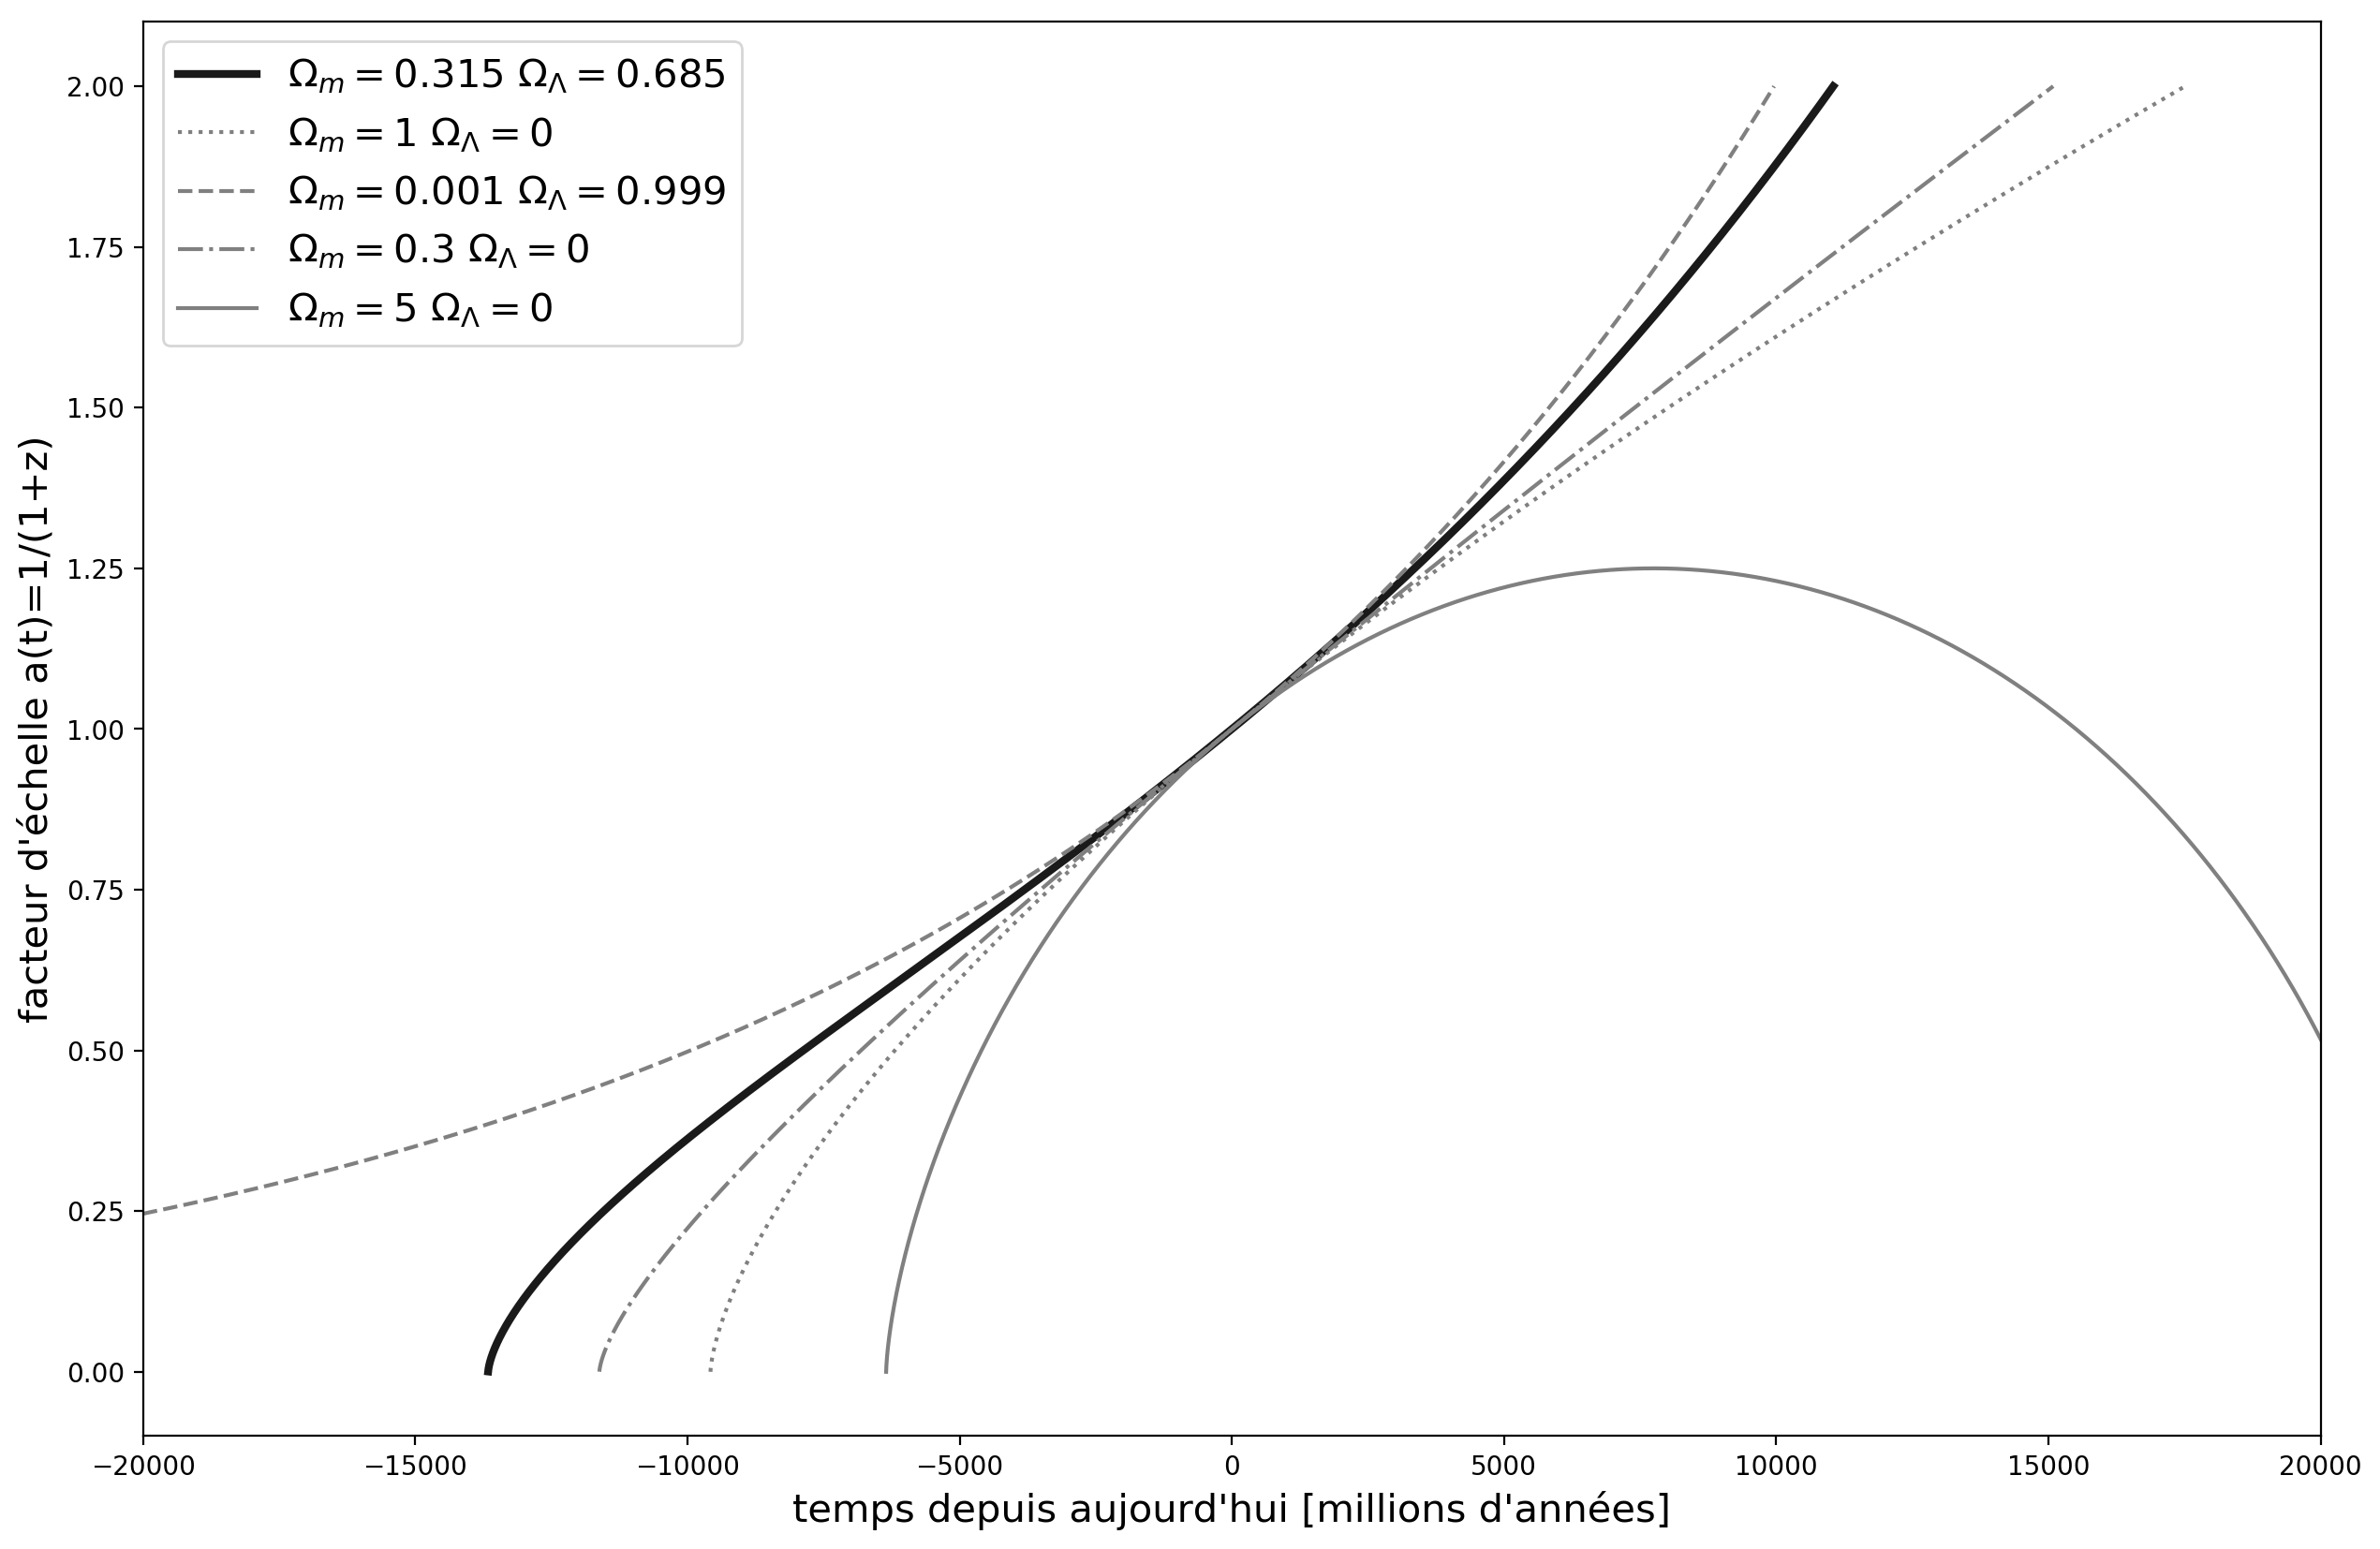
\includegraphics[height=10cm]{figs/a2t_cosmo.png}
	\caption{Evolution temporelle du facteur d'échelle $a(t)$ pour différentes cosmologies. Ici om désigne le paramètre de densité de la matière et ov désigne celui de l'énergie noire. Notez que le facteur d'échelle est normalisé à 1 pour $t=0$.}
	\label{f:aexpcosmo}
\end{figure}
%%!TEX root = /Users/domaubert/Documents/Lectures/cosmolog/cosmo_main.tex

\chapter{l'Univers Chaud}
Dans ce chapitre nous allons étudier de premières bases se rapportant à l'Univers quasi-primordial âgé de quelques minutes au plus. Durant cette période, la dynamique de l'Univers est régie par les espèces relativistes, avec une dépendance temporelle du facteur d'expansion en $a(t)\sim\sqrt{t}$~: durant ces époques les influences respectives de la matière et de la constante cosmologique sont faibles. Ces premiers instants sont proches du Big-Bang et l'Univers s'y trouve dense et chaud~: ces conditions sont propices aux interactions entre atomes et particules subatomiques. C'est durant cette époque que les abondances des particules reliques\index{particule relique} et des éléments légers\index{element légers@élément légers}\sidenote{terme qui désigne les éléments de faible nombre de masse tels que H, He, Li ou Be} sont fixées~: c'est de ces abondances dont nous allons discuter dans ce chapitre.

\section{Equilibre \& Gel de Réactions}
Les deux concepts fondamentaux des processus qui règlent les abondance\index{abondance} sont les notions \textit{d'abondance à l'équilibre}\index{abondance à l'équilibre} et de \textit{gel des réactions}\index{gel des réactions}. Dans notre cas, le terme d'abondance désigne la densité numérique d'une espèce atomique, subatomique, isotopique, etc... Par exemple l'abondance des atomes\index{atome} d'hydrogène se note $n_H$ et s'exprime en atomes par $m^3$. Les réactions qui permettent de modifier ces abondances font généralement intervenir d'autres réactifs. La photoionisation\index{ionisation} par exemple se caractérise par la réaction suivante:
\begin{equation}
n_H+\gamma \leftrightarrow n_{H+} + e^-,
\end{equation}
et dépend non seulement de l'abondance des atomes d'hydrogène\index{hydrogène} mais également de celle du nombre de photons\index{photon!UV} ionisants \sidenote{en l'occurrence surtout des photons ultra-violets}. Toutefois dans un très grand nombre de cas, la variation d'une espèce peut s'écrire comme ne dépendant que de sa propre abondance \textit{à l'équilibre} $n_e$ et d'un taux de réaction\index{taux de réaction} $\Gamma$ constant. Soit $n$ une abondance quelconque, son évolution pourra être suivie par une équation différentielle du type:
\begin{equation}
\frac{dn}{dt}=-\Gamma (n-n_e).
\end{equation}
Celle-ci est simple à comprendre. Si une abondance est déjà à l'équilibre\index{équilibre} $n=n_e$ et son abondance, par définition, ne varie pas. Si son abondance est supérieure à l'équilibre, le taux de réaction va agir comme une force de rappel\sidenote{on note que l'équation différentielle est similaire à celle décrivant la dynamique d'un ressort}, traduisant de fait une tendance à favoriser les réactions de destruction de l'espèce étudiée. A l'inverse si l'abondance est en déficit par rapport à l'équilibre, les réactions vont avoir tendance à la rétablir à des valeurs plus élevées. Notons que  l'inverse du taux de réactions fournit un temps caractéristique de retour à l'équilibre $t_e=\Gamma^{-1}$.

Toutefois il existe une autre manière de faire varier la densité numérique d'une espèce dans le contexte qui est le nôtre: il s'agit de la dilution cosmologique, déjà rencontrée dans le chapitre précédent. En effet, compte tenu de l'expansion de l'Univers\index{expansion}, si l'on dispose d'un certain nombre de particules d'un type donné dans un certain volume, sa \textit{densité} va évoluer même en l'absence de réaction (c'est à dire de destructions/créations). Ainsi la densité numérique d'une espèce donnée varie cosmologique de la façon suivante:
\begin{equation}
n=\frac{n_0}{a^3},
\end{equation}
ce qui ne fait que traduire l'équation différentielle suivante:
\begin{equation}
\frac{dn}{dt}=-3Hn,
\end{equation}
où $H$ est la fonction de Hubble usuelle \index{Hubble!fonction}, fonction du temps ou du paramètre d'expansion $H=\dot a/a$ \sidenote{le facteur 3 est typique de la dilution cosmologique d'une quantité \textit{volumique}, qui dépend du cube de la longueur}. Comme déjà indiqué, le temps de Hubble\index{Hubble!temps} $t_H=H^{-1}$ fournit le temps caractéristique d'évolution significative des distances dans le cosmos.

Dans le cas cosmologique général, les deux procédés se superposent et l'abondance d'une espèce arbitraire est régie par une équation de type:
\begin{equation}
\frac{dn}{dt}=-3Hn-\Gamma (n-n_e),
\label{e:reac}
\end{equation}
cette équation demande en toute généralité à être résolue numériquement. Toutefois 2 cas limites se détachent facilement:
\begin{itemize}
\item si $H\gg \Gamma$ : l'expansion est beaucoup plus efficace que les réactions. C'est un régime où le 2nd terme de l'équation \ref{e:reac} peut être négligé, on retrouve $n\sim a^{-3}$ et le nombre de particules dans un volume en expansion donné est \textit{constant}. On dit que l'espèce est \textit{gelée}.
\item si $H\ll \Gamma$ : on peut négliger la dilution cosmologique et les temps de retour à l'équilibre sont très courts. L'abondance est celle de l'équilibre, qui est éventuellement une fonction du temps $n\sim n_e(a)$.
\end{itemize}

En règle générale $H$ et $\Gamma$ sont tous deux fonctions du temps et $\Gamma$ a tendance à dominer au début de l'histoire de l'Univers (quand les densités et températures sont très élevées) pour être ensuite dominé par $H$. En effet à ces époques, la dynamique est dominée par le rayonnement et 
\begin{equation}
H\sim\frac{1}{a^2}
\end{equation}
tandis qu'un taux de réaction est du type $\Gamma\sim \sigma v n$ où $v\sim a^{-i}$ est une vitesse typique des réactifs, $\sigma$ une section efficace et $n\sim a^{-3}$ une densité volumique de réactifs. En supposant une section efficace de réaction constante, on a une dépendance de $Gamma$ en facteur d'expansion $a$ qui est au moins de l'ordre de :
\begin{equation}
\Gamma \sim \frac{1}{a^{3+i}}.
\end{equation}
La vitesse décroit avec la température, dont on verra qu'elle décroît avec le paramètre d'expansion $a$ et donnant $i>0$ : les taux de réactions dépendent plus fortement de l'histoire d'expansion pour dominer puis être dominés par $H$ au cours de la croissance de$a$. Par conséquent l'histoire typique de l'abondance d'une espèce suit d'abord celle de l'équilibre avant d'être gelée et n'être plus modifiée que par la dilution cosmologique. Cette transition porte le nom de "gel" ou \textit{freeze-out} en anglais\index{gel des réactions}.



\section{Statistique d'un gaz}
La question qui se pose à présent est celle de déterminer l'abondance à l'équilibre d'une espèce (hydrogène, photons, neutrinos, etc....). Celle-ci nous est donnée par la physique statistique\index{statistique d'un gaz}.

On se place dans le cas simple d'une particule libre\index{particule libre}\sidenote{non soumise à un potentiel extérieur}, auquel cas son énergie ne dépend que de son impulsion $\vec p$, ou bien de façon équivalente que de son vecteur d'onde\index{vecteur d'onde} $\vec k =\vec p /\hbar$ \sidenote{ici $\hbar=\frac{h}{2\pi}$ désigne la constante de Planck réduite}:
\begin{equation}
E^2=p^2c^2+m^2c^4=\hbar^2 c^2 k^2 +m^2c^4
\end{equation}
 Plus précisément l'énergie d'une particule ne dépend que de la norme $k$ du vecteur d'onde\index{nombre d'onde}. Par conséquent, l'ensemble des points dans l'espace des $\vec k$ qui fournissent une énergie donnée sont à l'intérieur d'une coquille de rayon $k$. De plus, le peuplement de cet espace est quantifié : en effet les nombres d'ondes accessibles (i.e. les impulsion accessibles) doivent être de la forme $\vec k = (n_x,n_y,n_z) 2\pi/L $ où $L$ désigne la taille de la "cuve" dans laquelle s'effectue l'étude et où le triplet est un triplet de valeurs entières. Par conséquent, une particule ne peut se trouver que sur les nœuds d'une maille pavant cet espace. 

Ces considérations nous permet d'évaluer le \textit{nombre d'états accessibles à une énergie E donnée}\index{nombre d'états}. Ce nombre est donné par le rapport entre le volume de l'espace des $\vec k$ à énergie $E$ donnée (la coquille):
\begin{equation}
4\pi k^2 dk
\end{equation} 
et le volume occupé par un état unique (le volume de la maille):
\begin{equation}
(2\pi/L)^3.
\end{equation}
On obtient alors le nombre d'états accessible à une particule libre d'énergie $E$ à $dE$ près \index{densité d'états}
\begin{equation}
N(E)dE=\frac{4\pi k^2 dk}{(2\pi/L)^3}.
\label{e:densetat}
\end{equation}

\begin{figure}[htbp]
	\centering
		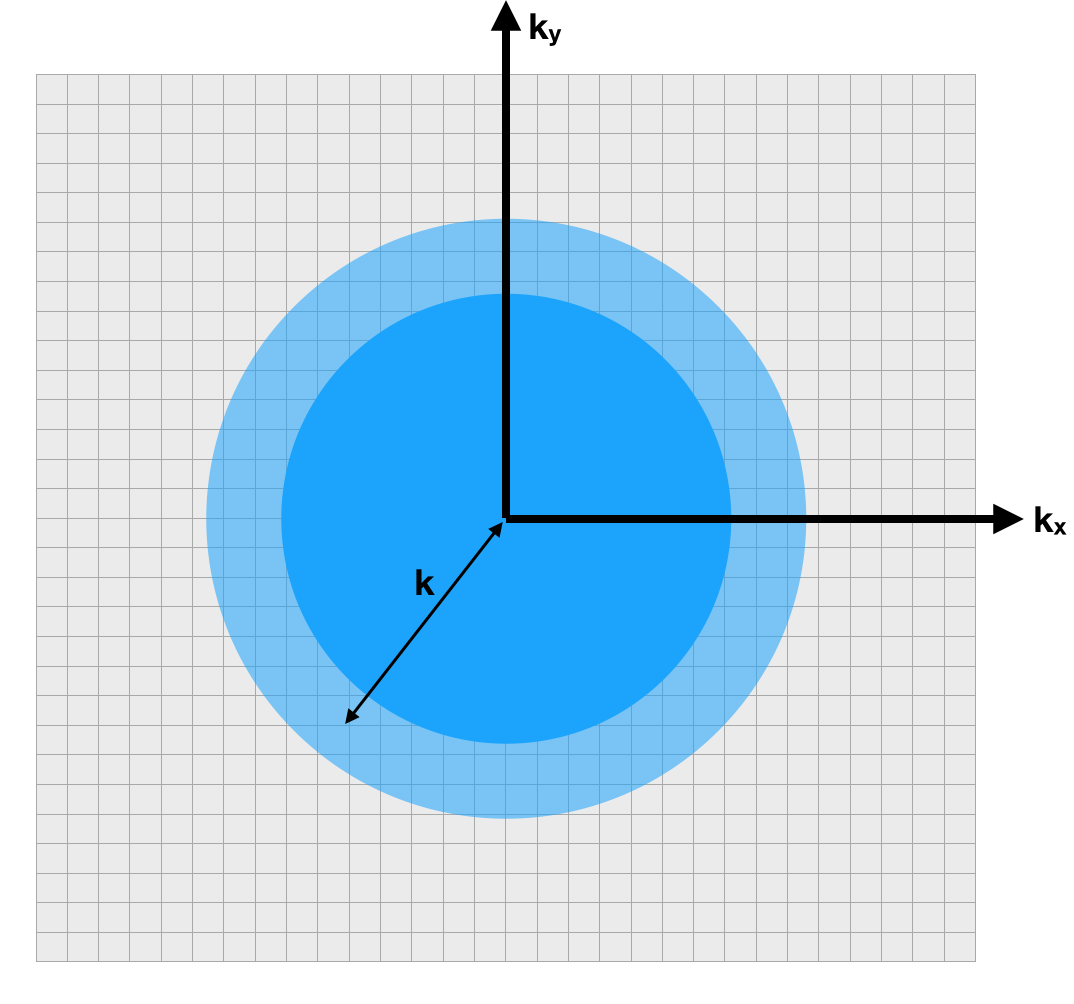
\includegraphics[height=12cm]{figs/k.png}
	\caption[Calcul de la densité d'état libres]{Comment calculer le nombre d'états d'énergie donnée ? Les états sont quantifiés et 'positionnés' sur une maille correspondant à des valeurs de $k_x$ et $k_y$ multiples de $2\pi/L$. Tous les états de même énergie partagent le même module $k$ : leur nombre est donc donné par la surface de la coquille ($2\pi k dk$) divisé par la surface d'un élément de la maille ($(2\pi/L)^2$). A 3D, ce nombre devient $4 \pi k^2 dk / (2\pi/L)^3$.}
	\label{f:k}
\end{figure}

L'équation \ref{e:densetat} n'est pas suffisante pour calculer l'abondance d'une particule: elle nous renseigne sur la quantité d'états accessible mais reste à déterminer combien de particules résident sur un état donné. Le \textit{niveau d'occupation}\index{niveau d'occupation d'un état} dépend du type de particule: si celle-ci est un fermion\index{fermion}\sidenote{une particule dont le spin est demi-entier comme l'électron ou  le proton} alors elle est soumise au principe d'exclusion de Pauli qui stipule qu'un état quantique donné ne peut être occupé, au plus, que par une particule. Si celle-ci est un boson\index{boson}\sidenote{une particule dont le spin est entier, comme le photon}, cette restriction ne s'applique pas. Plus précisément, les niveaux d'occupation sont donnés par les statistiques de Fermi-Dirac\index{Fermi-Dirac} et Bose-Einstein\index{Bose-Einstein}
\begin{equation}
n(E)=\frac{g(E)}{\exp(\beta(E-\mu))\pm 1}.
\label{e:BEFD}
\end{equation}
Le signe positif (resp. négatif) au dénominateur désigne la statistique de Fermi-Dirac\index{Fermi-Dirac!statistique} (resp. Bose-Einstein \index{Bose-Einstein!statistique}).La quantité $\beta=1/k_B T$ dépend est une représentation de la température\index{température}, $\mu$ est le potentiel chimique\index{potentiel chimique} de l'espèce étudiée et $g(E)$ est la dégénérescence\index{dégénerescence} d'un état d'énergie $E$. Cette dernière quantité dépend également de la particule considérée. On note que dans le cas d'une statistique de Fermi-Dirac, s'appliquant aux fermions, $n(E)\le g(E)$: cela découle du principe d'exclusion de Pauli\index{principe d'exclusion} l'occupation est au mieux égale à la dégénérescence du niveau d'énergie. A l'inverse les bosons, soumis à la statistique de Bose-Einstein, peuvent avoir des niveaux d'occupation arbitrairement grands.

A ce stade, l'abondance d'une particule peut être déterminée et le nombre total de particules d'une espèce donnée dans une cuve de volume $V=L^3$ à température $T$ est
\begin{equation}
N=\int_{E_{\mathrm{min}}}^\infty n(E)N(E) dE.
\label{e:abondance}
\end{equation}
Notons que cette intégrale porte sur toutes les énergies, depuis la plus faible jusqu'aux infinis. Cette valeur plancher de l'énergie dépend de la particule considérée. Par exemple pour une particule de masse nulle\sidenote{telle le photon}, on aura $E_\mathrm{min}=0$ tandis que pour une particule massive on aura $E_\mathrm{min}=mc^2$, correspondant à un état de repos (et donc d'impulsion minimale) absolu.

\section{Les photons}
Le cas des photons\index{photon} permet d'illustrer le calcul de la section précédente tout en étant d'une grande pertinence cosmologique: ils appartiennent aux particules dites relativistes et c'est elles qui dominent le budget numérique actuel de l'Univers. 

Le calcul de l'abondance des photons nécessite de préciser d'abord les quelques nombres nécessaires à sa bonne conduite. Dans un premier temps, les photons sont des particules de masse nulle, donc leur énergie est faite d'impulsion pure:
\begin{equation}
E_\gamma=pc=\hbar c k.
\end{equation} 
On rappelle que la densité d'états accessibles possédant une norme $k$ donnée a pour expression 
\begin{equation}
\frac{N(k)dk}{V}=\frac{4\pi k^2 dk}{V}\left(\frac{L}{2\pi}\right)^3=\frac{4\pi (E/\hbar c)^2 dE}{\hbar c V}\left(\frac{L}{2\pi}\right)^3.
\end{equation}
Par conséquent la densité volumique d'états d'énergie E accessible aux photons est donnée par:
\begin{equation}
\frac{N(E)dE}{V}=\frac{1}{2\pi^2}\frac{E^2dE}{(\hbar c)^3}.
\end{equation}
De plus le photon est sa propre antiparticule\index{antiparticule} et participe par exemple aux équations de désintégrations:
\begin{equation}
A + \bar{A} \leftrightarrow \gamma+\gamma.
\end{equation}
Or $\mu_A=-\mu_{\bar{A}}$ donc $\mu_\gamma=0$. Enfin le photon autorise deux hélicités par état d'énergie et possède un spin entier et obéit donc à la statistique de Bose-Einstein\index{Bose-Einstein!statistique}. L'état d'occupation d'un niveau d'énergie E est donc donné par :
\begin{equation}
n(E)=\frac{2}{e^{\frac{E}{k_B T}}-1}.
\end{equation}
D'où son abondance à l'équilibre:
\begin{equation}
n_\gamma=\frac{1}{(\hbar c)^3\pi^2}\int_0^\infty\frac{E^2dE}{e^{\frac{E}{k_B T}}-1}.
\end{equation}
On reconnait dans l'intégrale la distribution de Planck\index{Planck!distribution}, qui par définition décrit la distribution spectrale d'énergie d'un gaz de photons à l'équilibre, comme présent par exemple dans un corps noir\index{corps noir}. Cette intégrale peut être conduite analytiquement conduisant à \sidenote{en utilisant l'expression de la fonction \textit{zéta} de Riemann avec $\zeta(3)=\frac{1}{\Gamma(3)} \int_0^\infty \frac{x^2}{e^x-1}dx$.} :
\begin{equation}
n_\gamma \approx 0.244 \left(\frac{k_BT}{\hbar c}\right)^3 \mathrm{m}^{-3}.
\label{e:densphot}
\end{equation}

Aujourd'hui la température\index{température!gaz de photons} du gaz de photons du cosmos est de l'ordre de 2.73 K, correspondant à une densité de photons actuelle de :
\begin{equation}
n_\gamma\approx 410 \mathrm{cm}^{-3}.
\end{equation}
Pour mémoire, la densité d'atomes d'hydrogène\index{hydrogène!densité} actuelle (espèce qui domine la population de baryons) est de l'ordre de l'atome par $m^3$, on est donc dans un rapport de $10^{8-9}$,  extrêmement en faveur des photons. Une évaluation plus précise du rapport baryon/photon\index{rapport baryon/photon} $\eta$ est donnée par:
\begin{equation}
\eta \approx 5\times 10^{-10}\frac{\Omega_b h^2}{0.02}
\end{equation}
Cette surabondance de lumière résulte du processus de désintégration des particules massives que nous étudieront par la suite. 

\section{Histoire de la Température}

Si l'on examine à nouveau l'expression de la densité de photon (Eq. \ref{e:densphot}), on constate que celle ci varie en $n_\gamma \sim T^3$\index{photon!densité}. Ainsi si l'on considère une cuve de volume $V$ elle contient à un redshift $z$ donné le nombre de photons suivant:
\begin{equation}
N_\gamma(z) \sim V(z) T(z)^3.
\end{equation}
Or compte tenu de leur gigantesque domination numérique, ce nombre de photons doit être \textit{constant}: aucun processus (absorption/émission, à priori par des baryons extrêmement peu nombreux par rapport aux photons) ne peut changer $N_\gamma$ de façon significative. Toutefois, une cuve de taille donnée verra ses limites évoluer sous l'effet de la dynamique de l'Univers. En particulier $V=V_0 a^3$ d'où la loi d'évolution de la température des photons\index{température!photon}
\begin{equation}
T_\gamma=\frac{T_0}{a}=T_0 (1+z),
\end{equation}
avec $T_0=2.73K$. De plus compte tenu de la domination quasi totale des espèces relativistes sur le bilan numérique des particules du cosmos (comme illustrée par la valeur de $\eta$), on peut presque considérer que cette température est celle du cosmos. 

Une autre démonstration de cette relation repose sur le fait que le spectre doit conserver sa forme de courbe de Planck\index{Planck!distribution}, y compris sous l'effet de l'expansion, car c'est effectivement ce qui est observé aujourd'hui. Or le nombre de photons qui tombe dans une bande d'énergie $dE$ est, à une constante multiplicative près\sidenote{avec $V=a^3 V_0$ et $E=\frac{E_0}{a}$.},
\begin{equation}
V \frac{E^2 dE}{e^{\frac{E}{k_B T}}-1}=V_0 \frac{E_0^2 dE_0}{e^{\frac{E_0}{k_B aT}}-1}.
\end{equation}
Pour que le spectre reste inchangé, il faut 'neutraliser' la dernière dépendance en $a(t)$ qui se trouve dans le terme de l'exponentielle, en imposant que $a(t) T$ reste constant, redonnant ainsi l'expression précédente.


Aujourd'hui l'Univers est froid, mais par le passé celui-ci était plus chaud, en plus d'être plus dense comme expliqué dans les chapitres précédents. Notons pour finir que les photons du cosmos ne sont plus à l'équilibre thermodynamique à proprement parler depuis la production du fond diffus cosmologique\index{fond diffus cosmologique} : aujourd'hui ces photons n'interagissent plus avec les baryons, interactions qui auraient permis de maintenir le bain de photons à l'équilibre. Toutefois dans le passé plus chaud et plus dense, ces interactions existaient et un régime de fort couplage permettait de garantir un couplage matière rayonnement suffisant pour que la situation "thermodynamique" de l'Univers s'apparente à celle d'un corps noir\index{corps noir}. Cette situation a cessé (380 000 ans après le Big Bang comme nous le verrons) mais la domination des espèces relativistes est telle qu'aucun processus n'est en mesure de changer significativement la fonction de distribution des photons: en l'absence de processus permettant cette modification, le gaz de photons a pu conserver la mémoire d'une période antérieure d'équilibre thermodynamique\index{équilibre!thermodynamique}.

Par la suite nous considèrerons des époques durant lesquelles le bilan énergétique de l'Univers est dominé par les espèces relativistes durant lesquelles le facteur d'expansion varie en :
\begin{equation}
a\sim \sqrt t.
\end{equation}
Il en découle les lois d'échelles suivantes \sidenote{on rappelle que le MeV désigne 1 million d'électrons-volts et constitue une énergie équivalente à $1 MeV \sim 1.6 \times 10^{13} J$}:
\begin{equation}
T\approx\frac{10^{10} K}{\sqrt{t\mathrm{(sec)}}} \approx \frac{1}{k_B}\frac{1 \mathrm{MeV}}{\sqrt{t\mathrm{(sec)}}}.
\end{equation}
Ces lois permettent déjà de se faire une idée des hautes températures en place durant les phases primordiales de l'Univers et donc permettent d'anticiper que des processus très énergétiques sont en mesure d'être effectifs. Par exemple les énergies typiques du LHC\index{LHC} sont de l'ordre du TeV $=1e6$ MeV: elles correspondent aux énergies typiques dans un Univers de $10^{-12}$ secondes. De plus ces lois d'échelles permettent d'anticiper que certaines époques joueront un rôle pour certaines particules quand l'énergie typique du cosmos est de l'ordre de leur énergie de masse : par exemple l'électron\index{electron@électron} possède une énergie de masse proche du MeV ( 511 keV exactement) et donc il est probable que son abondance soit significativement modifiée lorsque l'Univers aura un âge correspondant à cette masse (à savoir de l'ordre de la seconde).


\section{Evolution des abondances}
Pour une "particule" quelconque, l'expression précise de son abondance\index{abondance} va dépendre de son caractère relativiste ou non. Il existe des particules pour lesquelles ce caractère reste inchangé au cours du temps, comme les photons par exemples, mais en général, une particule aura tendance à être considérée comme relativiste aux premiers instants de l'Univers puis évoluera plus tard vers le régime non-relativiste, avec comme conséquence une variation, parfois radicale, de son abondance au cours du temps.

L'énergie d'une particule libre\index{particule libre} est donnée par :
\begin{equation}
E=\sqrt{p^2c^2+m^2c^4}.
\end{equation}
 Une particule est dite \textit{ultra-relativiste}\index{particule!ultra-relativiste} si son énergie de masse\index{energie@énergie!masse} est considérée comme négligeable devant son énergie cinétique\index{energie@énergie!cinétique}, $pc\gg mc^2$, auquel cas $E\sim pc$. C'est notamment le cas du photon, étudié en détail dans la section précédente. A l'inverse, une particule est dite \textit{non-relativiste}\index{particule!non-relativiste} si son énergie de masse constitue l'essentiel de son énergie totale $pc \ll mc^2$. Cela correspond au fluide "matière" développé dans le chapitre précédent et dans ce cas $E\sim mc^2 (1+ p^2/2m) \sim mc^2$. L'utilisation de l'une ou l'autre de ces expressions pour l'énergie dans l'équation \ref{e:abondance} va conduire à des expressions différentes des abondances.
 
 \paragraph{Cas ultra-relativiste\index{particule!ultra-relativiste}}
Ce cas correspond à celui étudié précédemment pour les photons : en effet, si l'on parle du principe que la masse d'une particule est négligeable, elle en devient quasi similaire à un photon et son abondance n'en diffère que par le facteur de dégénérescence et par la statistique à utiliser (BE ou FD). En conséquence, l'abondance d'une particule dans ce régime ultra-relativiste sera proche de celle des photons. Un calcul précis donne l'abondance suivante pour un \textit{boson}\index{boson}
\begin{equation}
n_B=n_\gamma\frac{g_B}{2},
\end{equation}
tandis que si la particule étudiée est un fermion\index{fermion}
\begin{equation}
n_F=n_\gamma\frac{3g_F}{8}.
\end{equation}
A un facteur proche de l'unité près, l'abondance d'une particule relativiste est essentiellement celle des photons $n\sim n_\gamma$.

\paragraph{Cas non relativiste\index{particule!non-relativiste}}
Dans ce régime, l'énergie d'une particule est la somme de l'énergie cinétique classique et de son énergie de masse, $E\sim p^2/2m +mc^2$ et l'occupation statistique des énergies (cf. eq. \ref{e:BEFD}) devient la statistique de  Maxwell-Boltzmann\index{Maxwell-Boltzmann!statistique}, donnée par\sidenote{généralement cette statistique devient valable quand $e^{\frac{\min{E}-\mu}{k_B T}}\ll 1$. Or on verra ci-dessous que ce régime non relativiste est précisément décrit par une température faible devant l'énergie de masse $k_BT \ll mc^2$ avec $\min E =mc^2$}:
\begin{equation}
g e^{-\frac{E-\mu}{k_B T}}.
\end{equation}
 L'abondance est alors donnée par l'expression suivante \sidenote{on note que l'intégrale porte sur $\infty$ alors qu'elle devrait être bornée pour satisfaire l'hypothèse non-relativiste. Toutefois, l'intégrand est une gaussienne dont la décroissance est très rapide : l'erreur est donc faible et permet de reconnaître l'expression de la (moitié de la) variance d'une distribution normale.}
\begin{equation}
n=\frac{g}{2\pi^2 \hbar^3}e^{-\frac{mc^2-\mu}{k_BT}}\int_0^\infty p^2 e^{-\frac{p^2}{2mk_B T}}dp.
\end{equation} 
 Le calcul de son abondance donne une quantité qui dépend directement de la température\index{température}
\begin{equation}
n=ge^{\frac{\mu}{k_BT}}\left(\frac{m k_B T}{2\pi\hbar^2}\right)^{3/2}e^{-\frac{mc^2}{k_B T}}\sim e^{-\frac{mc^2}{k_B T}}.
\label{e:nonrel}
\end{equation}


Compte tenu de l'évolution de la température, qui décroit avec le temps, l'abondance décroît de façon exponentielle. La réaction typique permettant cette décroissance est une réaction de \textit{désintégration}:
\begin{equation}
A+\bar A \leftrightarrow \gamma+\gamma,
\end{equation}
avec un déplacement de l'équilibre vers la droite de cette équation, i.e. vers le réservoir de photons.

\paragraph{Transition}
Se pose alors la question de la détermination du régime dans lequel se trouve une particule. Il s'avère que la température d'un gaz de particule est liée à l'énergie cinétique et $E_c\sim k_B T$. Par conséquent à haute température, $k_B T\gg mc^2$, une particule tend à être ultra-relativiste\sidenote{on a la vitesse $v\sim\sqrt{k_B T}$ qui tend à devenir non-négligeable devant $c$.} tandis qu' à basse température $k_B T\ll mc^2$, celle-ci tend à être non relativiste. On sait également que la température de l'Univers décroît au cours du temps, donc pour une particule massive donnée, il se trouvera toujours une époque reculée où cette particule est relativiste, suivie par une époque où elle basculera dans le régime non-relativiste. La transition entre les deux régimes opère lorsque l'énergie cinétique typique est de l'ordre de l'énergie de masse\index{energie@énergie!masse}
\begin{equation}
k_B T(z^*)=mc^2.
\end{equation}
Sachant que la température du rayonnement\index{température!rayonnement} varie en $T_\gamma\sim (1+z)$ et qu'à l'équilibre un fort couplage existe, la transition opère à un redshift $z^*$ donné par :
\begin{equation}
1+z^*=\frac{mc^2}{k_B T_0}.
\end{equation}
 On constate ainsi qu'une particule passera dans le régime non relativiste d'autant plus rapidement qu'elle sera massive. A l'inverse, une particule de masse nulle ne pourra jamais, comme attendu, basculer dans le régime non relativiste.
 

 
 \section{Abondances résiduelles}
 
\begin{figure}[htbp]
	\centering
		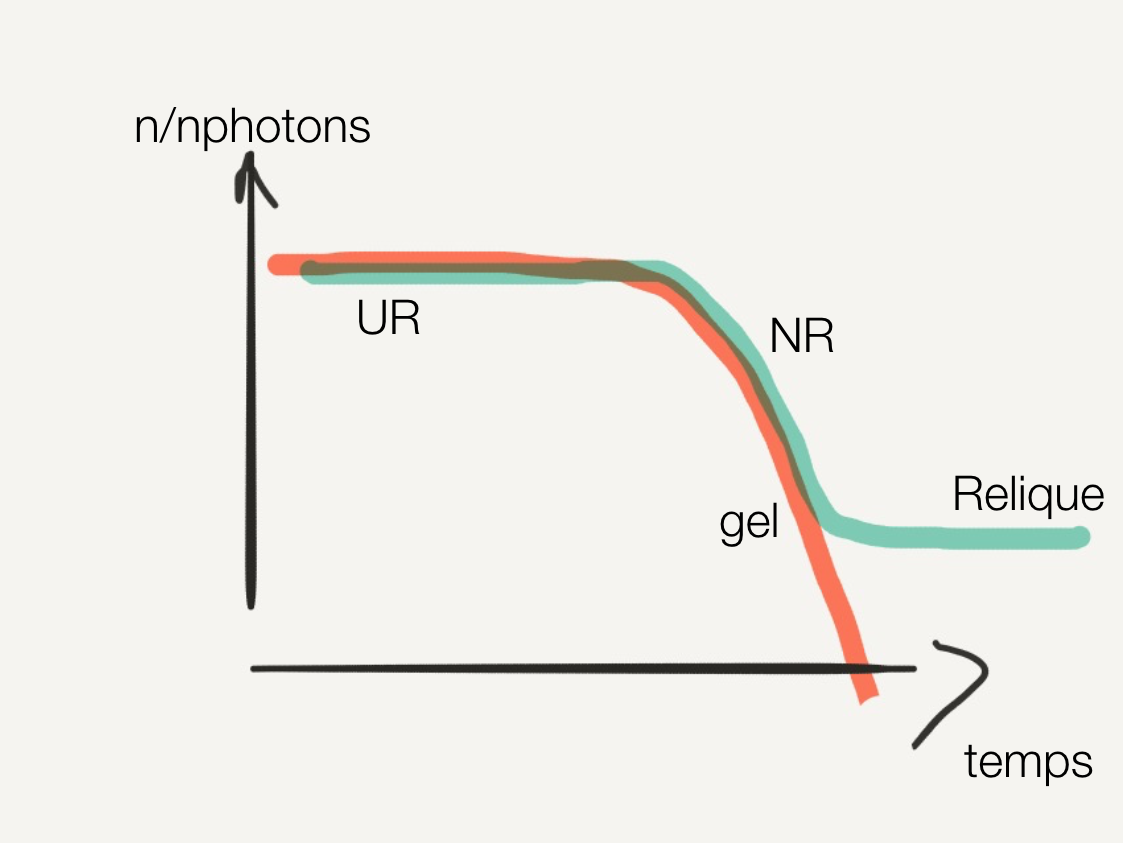
\includegraphics[height=12cm]{figs/freeze.png}
	\caption[Evolution schématique de l'abondance d'une particule relique.]{Evolution schématique de l'abondance d'une particule relique. Dans le régime ultra-relativiste (UR), la particule se comporte comme un photon et son abondance est similaire. Le passage au régime non relativiste (NR) provoque la décroissance de l'abondance, exponentielle, typique d'une particule massive. Son abondance deviendrait négligeable sans le 'gel' (freeze-out)~: la dilution cosmologique ainsi que l'absence de réactifs ou la baisse de température vont stabiliser la densité numérique de la particule à une abondance non nulle. }
	\label{f:freeze}
\end{figure}
 
 
  En résumé, l'abondance\index{abondance!à l'équilibre} à l'équilibre d'une particule passe par 2 étapes distinctes:
 \begin{itemize}
 \item à grand $z>z^*$, nous avons $k_B T \gg mc^2$ et $n\sim n_\gamma$
 \item à bas  $z<z^*$, nous avons $k_B T \ll mc^2$ et l'abondance décroît de façon exponentielle. Elle se désintègre et son abondance devient très inférieure à l'abondance des photons, $n\ll n_\gamma$.
 \end{itemize}
Or nous avons vu précédemment que les réactions qui permettent le maintien de cet équilibre vont "geler"\index{gel des réactions}\sidenote{appelé aussi \textit{Freeze-out}} et découpler une espèce de la "soupe" de particules en interaction: après ce gel, l'abondance d'une espèce va rester celle de l'équilibre au moment du découplage. Ce gel peut opérer avant ou après $z^*$. Si une particule gèle pour $z>z^*$, elle se trouvait dans son régime relativiste, en grande abondance. Un tel type de particule va rester très abondante jusqu'à nos jours et c'est par exemple le cas des neutrinos\index{neutrinos}. Si à l'inverse elle gèle pour $z<z^*$, alors celle-ci avait déjà entamé sa désintégration durant laquelle son abondance décroît de façon exponentielle. Par conséquent la particule est en très faible abondance et aujourd'hui son abondance doit être très faible devant celle des photons (et donc des neutrinos). C'est le scénario essentiellement de toutes les particules massives, que l'on appelle aussi \textit{particules reliques}\index{particules reliques} car elles auront survécu à ce processus.
 
 \section{Asymétrie Matière-Antimatière\index{asymétrie matière-antimatière}\index{antimatière}}
Pour conclure ces considérations sur la physique de l'Univers chaud et énergétique, quelques mots sur l'asymétrie matière-antimatière. Les baryons ont un nombre quantique baryonique de valeur +1 et on peut leur associer des \textit{antibaryons}, de nombre baryonique -1 : le proton et le neutron possèdent ainsi des antibaryons que sont l'antiproton et l'antineutron \sidenote{dans le cas de l'antiproton, cela se manifeste notamment par une charge électrique opposée et donc négative}. Au delà de ces considérations sur ces nombres quantiques, l'assemblage d'antibaryons permet de faire de l'antimatière qui en tout autre point ressemble beaucoup à la matière normale : ces 2 types opposés partagent par exemple la même masse et toute réaction de type matière peut en principe être réalisée dans sa version antimatière \sidenote{on parle de réaction conjuguée}.

Lorsque les particules reliques sont en phase de désintégration et voient leurs abondances chuter de façon exponentielle, l'un des canaux privilégié de cette baisse est précisément le processus d'annihilation\index{annihilation} matière-antimatière. Soit une particule $A$ et son antiparticule $\bar A$, leur éventuelle rencontre conduit à la production d'énergie pure sous forme de photons:
\begin{equation}
A+ \bar A \leftrightarrow \gamma.
\end{equation}
 Ce processus est extrêmement efficace et on peut montrer qu'en cas d'abondance initiale égale entre particules et antiparticules, l'abondance des particules reliques devraient être de l'ordre de :
 \begin{equation}
 \eta=\frac{n_B}{n_\gamma}\sim10^{-18}
 \end{equation}
 or nous venons de voir que l'ordre de grandeur observé actuellement du rapport baryons sur photons $\eta$ est environ $10^9$ plus grand. Ceci suggère fortement que le gel des abondances des baryons a été dicté par l'absence de réactifs de type antibaryons plutôt que par une perte d'efficacité de la réaction, avec un excès en faveur de la matière de l'ordre de :
 \begin{equation}
 \frac{n_A-n_{\bar A}}{n_A+n_{\bar A}}\sim10^{-9}.
 \end{equation}
 Par ailleurs, nous constatons autour de nous une absence d'abondance significative d'antimatière, qui autrement se manifesterait par la production de photons gamma à très haute énergie lors de rencontre avec la matière \sidenote{les photons produits par les annihilation emportent une énergie $mc^2$, donc de l'ordre du GeV pour des protons-antiprotons par exemple.} Tout indique qu'il existait une asymétrie dans les abondances initiales de particules et d'antiparticules, faible mais non nulle et suffisante pour que notre Univers soit aujourd'hui dominé par la matière.
 
Ceci étant posé, comment expliquer une telle asymétrie ? Une première possibilité est qu'il s'agisse simplement d'une des caractéristique de notre Univers. Une seconde possibilité est qu'il existe des mécanismes qui sont capables de transformer une situation initialement symétrique en situation présentant une légère surabondance de matière : ces processus auraient étés à l'oeuvre lors d'un évènement que l'on nomme la \textit{Baryogénèse}\index{Baryogénèse}. Aujourd'hui, nous ne savons pas quand elle a eu lieu\sidenote{si elle a eu lieu} et sous quelles modalités exactes : par contre dès 1967, Sakharov posa 3 conditions\index{conditions de Sakharov} qui doivent être satisfaites à minima pour que la Baryogénèse ait pu prendre place :
\begin{enumerate}
\item il faut des réactions qui ne conservent pas le nombre baryonique:
\begin{eqnarray}
A + \bar B &\leftrightarrow& C
\end{eqnarray}
C'est une condition minimale pour qu'une situation symétrique puisse évoluer vers une asymétrie.
\item il faut que les réactions conjuguées aient des taux de réactions différents.
\begin{eqnarray}
A + \bar B &\leftrightarrow& C\\
\bar A + B &\leftrightarrow& \bar C.
\end{eqnarray}
En effet, pour une réaction qui ne conserve pas le nombre baryonique, la réaction conjuguée est également possible : si elles sont toutes aussi efficaces, le nombre baryonique global reste nul et la symétrie n'est pas brisée.
\item si les 2 conditions précédentes sont réalisées, nous obtenons une population en $C$ et $\bar C$ asymétrique. Toutefois, il ne faut pas l'équilibre thermodynamique soit maintenu : comme vu précédemment l'abondance d'une particule à l'équilibre ne dépend que de sa masse, qui est identique pour les 2 types de matière. Il faut figer le déséquilibre créé et par exemple empêcher que nos réactions puissent retourner à l'état initial symétrique:
\begin{eqnarray}
A + \bar B &\rightarrow& C\\
\bar A + B &\rightarrow& \bar C.
\end{eqnarray}
\end{enumerate}
\begin{figure}[htbp]
	\centering
		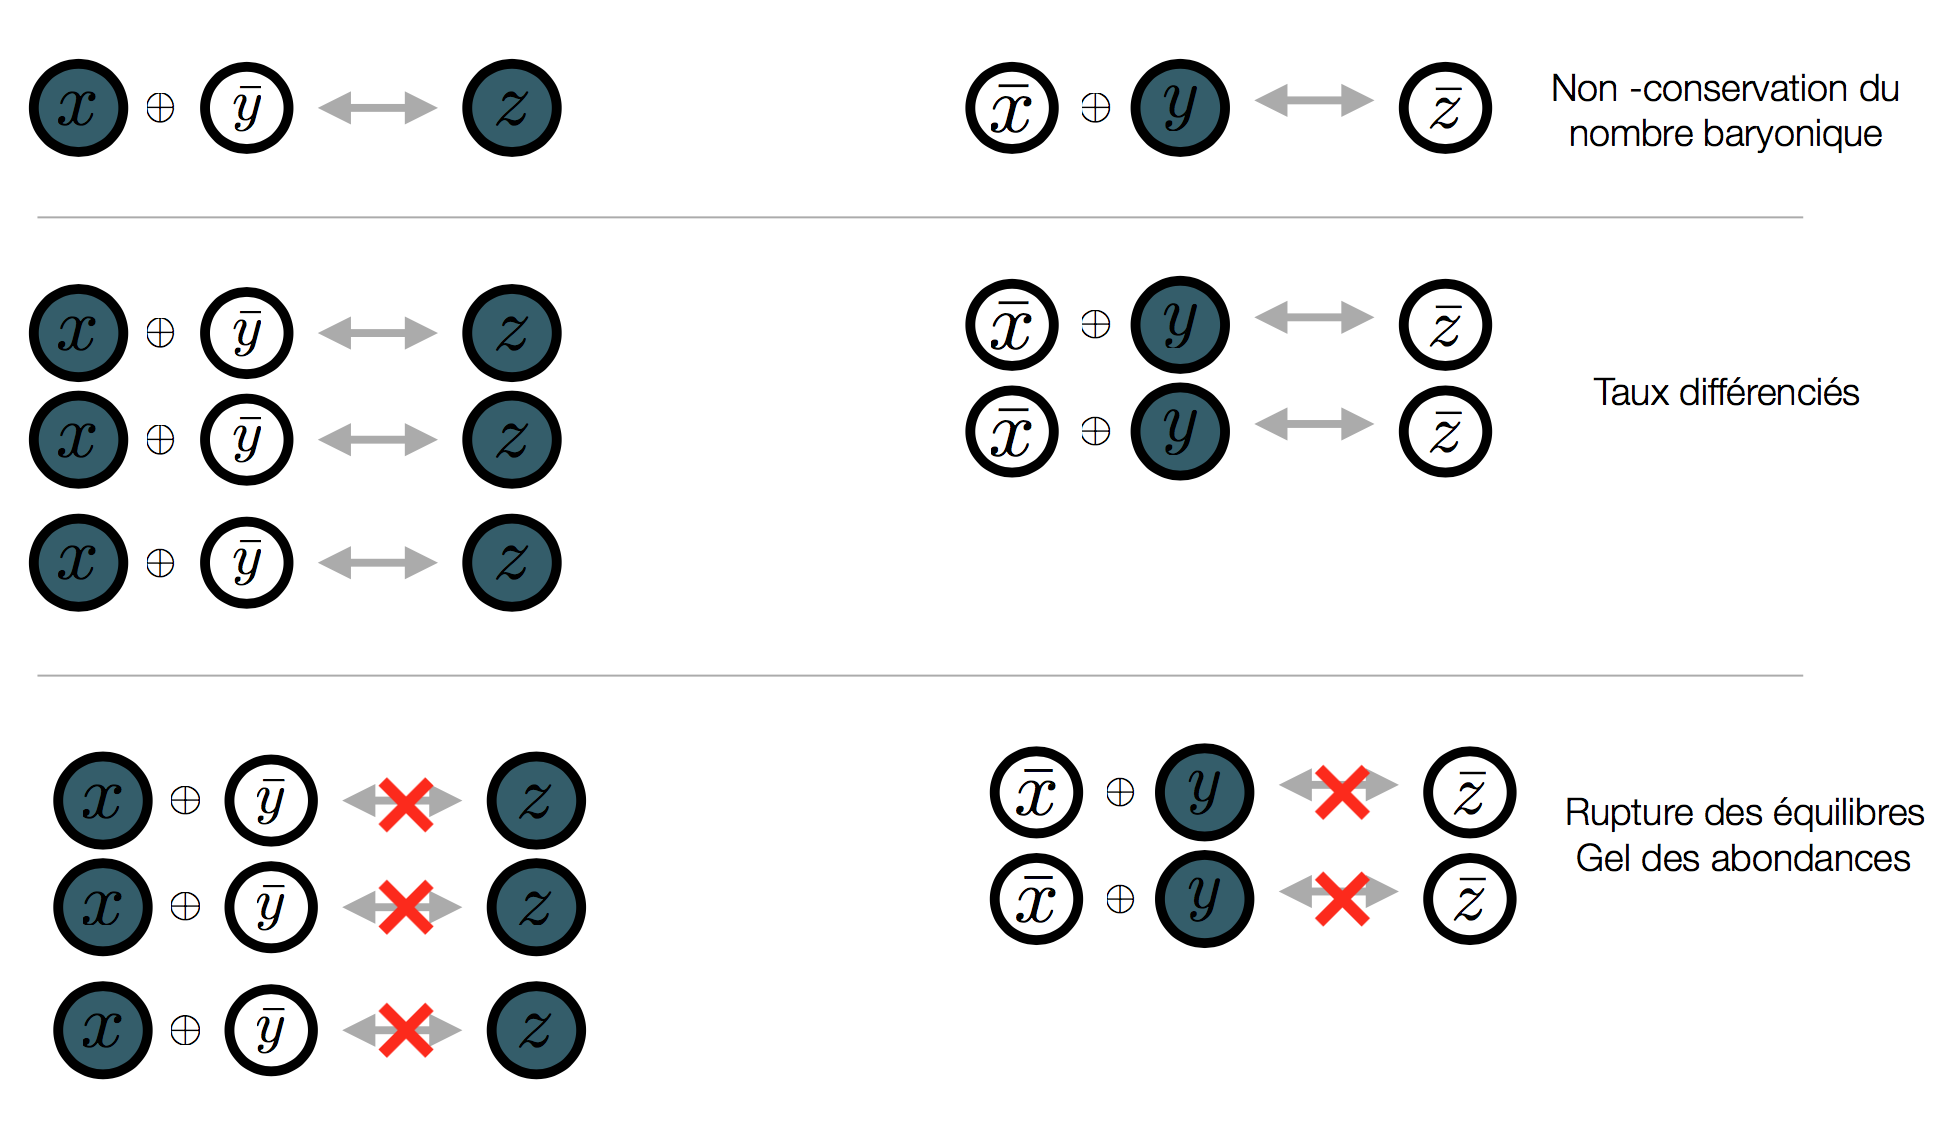
\includegraphics[height=12cm]{figs/sakharov.png}
	\caption[Les conditions de Sakharov]{Les conditions de Sakharov, nécessaires à l'existence d'une Baryogénèse à l'origine de l'asymétrie matière-antimatière. Il faut des réactions qui ne conservent pas le nombre de baryons, qui opèrent à des taux différents quand elles sont réalisées avec de l'antimatière et un procédé qui gèle l'équilibre thermodynamique et conserve l'asymétrie conservée. Initialement, l'abondance des particules $x,\bar x, y, \bar y$ présentait une symétrie matière-antimatière, symétrie qui est brisée pour l'abondance finale des particules $z$ et $\bar z$.}
	\label{f:sakharov}
\end{figure}

 Il s'avère que ces 3 conditions sont réunies dans la nature. Il existe des réactions qui ne conservent pas le nombre baryonique (condition 1), les taux de réaction des transformations conjuguées sont différenciées (condition 2)\sidenote{c'est notamment ce qui est testé lors des mesures de violations de conjugaison-parité (CP) dans les grands accélérateurs} et pour finir l'Univers, en particulier à cause de la baisse de température induite par l'expansion, fait régulièrement sortir des particules de l'équilibre thermodynamique en gelant les interactions. Ces conditions sont nécessaires mais non suffisantes : aujourd'hui la Baryogénèse apparaît comme une possibilité de principe mais dont on ne sait pas actuellement si elle a eu lieu et dans quelles conditions.
 
%%!TEX root = /Users/domaubert/Documents/Lectures/cosmologie/cosmo_main.tex

\chapter{Histoire thermique de l'Univers et Nucléosynthèse primordiale}

Dans ce chapitre nous allons voir comment les processus à l'œuvre dans l'Univers chaud vont conduire aux abondances observées actuellement des principales particules élémentaires et des éléments légers. Ces processus se déroulent pour $t<3$ minutes, dans un Univers dont la dynamique est dominée par les espèces relativistes.

\section{Quelques étapes}
On rappelle que 2 processus sont en compétition: l'annihilation qui tend à faire décroître de façon exponentielle l'abondance d'une particule donnée et le gel qui tend à figer l'abondance de cette particule en la soustrayant au bain de réactions environnant. La séquence suivante donne un aperçu de la cascade de processus qui opèrent lors de la baisse de température de l'Univers, induite par l'expansion ($T=T_0(1+z)$). La séquence suivante démarre au confinement des quarks dans les nucléons.
\newline
\begin{itemize}
\item $T\sim 3\cdot 10^{12}$ K : ($t\sim 10^{-5}$ sec , $kT \sim 250$ MeV) : confinement des quarks. Particules présentes $p,n, \pi^+,\pi^0, \pi^-, e,\bar e, \mu \bar \mu$ + neutrinos ($\nu_e,\bar \nu_e, \nu_\mu, \bar \nu_\mu$).\\
Les particules $\tau, \bar \tau$ sont déjà annihilées à ce stade et les neutrinos associés $\nu_\tau, \bar \nu_\tau$ sont gelés.
 \item $T\sim 10^{12}$ K : désintégration des pions
 \item $T\sim 10^{11}$ K : désintégration des muons et gel des neutrinos associés
 \item $T\sim 6 \cdot 10^{9}$ K : ($kT \sim 500$ keV, t$\sim 1$ s) désintégrations des électrons. Gel des $\nu_e$ et gel des abondances relatives de $n$ et $p$.
 \item $T\sim 10^9$ K : démarrage de la nucléosynthèse
 \item $T\sim 3000$ K : recombinaison, production du fond diffus
\end{itemize}

\paragraph{Entropie et fond neutrino} 
Parmi les étapes mentionnées précédemment on constate que les neutrinos se découplent de la 'soupe cosmique' en des époques très réculées et toujours dans leur régime relativiste. Lors du passage des électrons dans le régime non relativiste (qui opère plus tard), ces même neutrinos ne peuvent donc servir de canaux de désintégration car ils n'intéragissent plus avec ceux-ci via l'interaction faible. Cette désintégration se fait donc uniquement suivant:
\begin{equation}
e^-+e^+\rightarrow \gamma
\end{equation}
Ce processus opère à entropie constante, donc l'entropie des électrons est reversée sur les photons et non vers le neutrinos. On peut montrer que la densité d'entropie de bosons et fermions sont reliées par:
\begin{equation}
s_F=\frac{7}{8}\frac{g_F}{g_B} s_B
\end{equation}
Par conséquent la nouvelle entropie des photons, post-anihilation des électrons est :
\begin{equation}
s'_\gamma=s_\gamma+s_{e+}+s_{e-}=\frac{11}{4}s_\gamma.
\end{equation}
De plus l'entropie d'une espèce relativiste est une fonction directe du cube de sa température. Donc nous avons d'une part une espèce relativiste qui aura évolué de façon passive  (les neutrinos avec $s'_\nu=s_\nu$) et une autre qui aura augmenté grâce aux électrons. Donc en fin de désintégration :
\begin{equation}
s'_\gamma=\frac{11}{4} s_\nu
\end{equation}
ou bien
\begin{equation}
T_\nu=\left(\frac{4}{11}\right)^{1/3} T_\gamma
\end{equation}
Le gaz de neutrino doit être plus froid que celui de photons. Le fond neutrino peut en principe être mesuré aujourd'hui (même si cela reste encore pratiquement impossible) et doit donc présenter une température de  $T_{\nu,0}=1.95 K$.

\section{Synthèse de l'hélium}
La synthèse de l'hélium constitue l'évènement majeur de la production des éléments légers lors de la phase chaude du Big-Bang. L'abondance finale de cet élément va essentiellement dépendre du matériau à disposition et donc de la quantité de nucléons disponible.

\paragraph{Rapport neutron/proton}
 Environ 1 seconde après le Big-Bang, les nucléons (protons et neutrons) ne sont plus relativistes et leurs abondances (notées $p$ et $n$ respectivement pour les protons et neutrons) sont régies par une statistique de type Maxwell-Boltzmann:
\begin{equation}
p\approx n \sim e^{-\frac{m_p c^2}{k_B T}}.
\end{equation}
Les abondances des deux nucléons suivent des évolutions similaires car leurs masses sont proches : le proton est constitué du triplet de quarks $uud$  et possède une masse de $m_p=938.27$ MeV, tandis que le neutron est composé du triplet $udd$, pour une masse $m_n=939.56$ MeV. En toute rigueur néanmoins, l'écart de masse $\Delta m=m_n-m_p=1.3$ MeV suffit pour favoriser l'abondance du proton par rapport à celle du neutron, dont l'évolution en abondance est plus rapide. Le rapport d'abondance est donné par:
\begin{equation}
\frac{n}{p}=e^{-\frac{\Delta m}{k_B T}},
\end{equation}
Le gel des réactions impliquant neutrons et protons se produit environ 2 secondes après le Big-Bang. A cet instant le rapport neutrons sur protons vaut:
\begin{equation}
\left(\frac{n}{p}\right)_\mathrm{gel}\approx\frac{1}{6}.
\end{equation}

\paragraph{Synthèse du Deutérium}
Le Deutérium est un noyau composé d'un proton et d'un neutron et il fait office d'étape intermédiaire vers la production d'hélium. La production de cet élément se fait via la réaction:
\begin{equation}
p+n\leftrightarrow D+\gamma ,
\label{e:deut}
\end{equation}
cette équation doit satisfaire l'équilibre des potentiels chimiques:
\begin{equation}
\mu_p +\mu_n =\mu_D (+0).
\end{equation}
A partir de l'équation \ref{e:nonrel}, ces potentiels chimiques peuvent être extraits pour chaque espèce. En appliquant alors l'égalité des potentiels on obtient l'équation de Saha:
\begin{equation}
X_D=n \times \frac{g_D}{g_n g_p} \left(\frac{2\pi \hbar^2}{kT}\right)^{3/2}\left(\frac{m_D}{m_n m_p}\right)^{3/2} \times e^{\frac{B}{kT}},
\end{equation}
où $X_D=\frac{n_D}{p}$ est le rapport deutérium sur proton et $B=2.22$ MeV est l'énergie de liaison de l'élément. Il est d'usage d'exprimer l'abondance de neutrons $n$ en fonction de l'abondance de photons $n\sim \eta n_\gamma$:
\begin{equation}
n\approx 0.244 \eta \left(\frac{k_BT}{\hbar c}\right)^3.
\end{equation}
La dépendance globale de l'abondance du deutérium peut alors se résumer à:
\begin{equation}
X_D\sim(k_BT)^{3/2}\eta e^{\frac{B}{k_B T}}.
\label{e:saha}
\end{equation}
Il apparaît une énergie caractéristique donnée par l'énergie de liaison $B\approx 2$ MeV~: à première vue, en se plaçant quelques secondes après le Big-Bang, la température a suffisamment baissé pour pour que le deutérium devienne suffisamment abondant, via le terme exponentiel de l'équation de Saha. Toutefois les réactifs sont peu abondants ou à l'inverse les photons sont extrêmement nombreux et empêche un déplacement significatif de l'équation \ref{e:deut} vers la production de deutérium : dans l'équation \ref{e:saha} cela se manifeste par le terme $\eta \ll 1$ qui amortit le terme exponentiel. Il faut donc attendre une évolution significative de la température pour que in fine le deutérium puisse être produit en quantité abondante. Ce blocage au niveau du deutérium au cours de la chaîne de synthèse de l'hélium constitue un goulot d'étranglement: on parle de \textit{deutérium bottleneck}.

\paragraph{radioactivité $\beta$} En pratique il faut attendre environ 100 secondes, au bout duquel $k_B T\sim 0.1$ MeV pour que l'abondance de deutérium soit suffisante pour poursuivre la synthèse des éléments légers. Pendant ce délai, le rapport $n/p$ continue de décroît sous l'effet de la radioactivité $\beta$ qui conduit à la transformation de neutrons en protons via l'émission d'électrons. La durée de vie du neutron étant de l'ordre de 15 minutes, la modification du rapport est faible mais réelle. A la fin du deutérium bottleneck, nous avons:
\begin{equation}
\left(\frac{n}{p}\right)_\mathrm{bottleneck} \sim \frac{1}{7}
\end{equation}

\paragraph{synthèse de l'hélium et autres éléments légers}
Le deutérium devenant disponible, l'hélium peut être synthétisé. L'énergie de liaison de ce noyau est très importante $B_{He}\sim 30$ MeV, la synthèse est quasi immédiate et quasi totale quand les températures typiques sont de l'ordre de $k_B T < 0.1$ MeV : l'intégralité des neutrons se trouvent piégés dans les noyaux d'hélium (2 protons + 2 neutrons). Disposant à cet instant de 7 protons pour chaque neutrons, cela conduit à une fraction de masse sous forme d'hélium donnée par
\begin{equation}
Y_\mathrm{He}\sim 25\%
\end{equation}
En nombre, l'hélium représente seulement $10\%$ des noyaux, le reste étant quasi-exclusivement des protons, i.e. des noyaux d'hydrogène.

\begin{figure}[htbp]
	\centering
		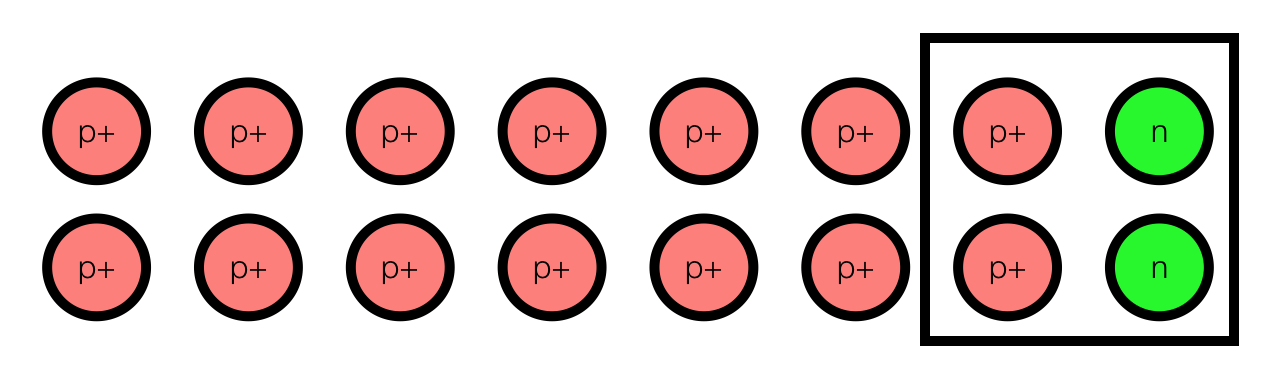
\includegraphics[height=12cm]{figs/helium.png}
	\caption{La situation après la fin du goulot du 'Deutérium'. Chaque groupe de 8 nucléons contient environ 1 neutron : un noyau d'hélium peut donc être fabriqué pour 16 nucléons, donnant un rapport de masse final d'environ 25\%.}
	\label{f:helium}
\end{figure}

Quelques éléments supplémentaires sont également produits. Par exemple le Li$^7$ est un élément produit en faible quantité à partir de l'hélium, ainsi que He$^3$ qui est un résidu des réaction de production de He$^4$. D'autres éléments comme Be$^7$ et H$^3$ sont également synthétisés mais leur temps de vie courts par rapport à l'âge de l'Univers font que ces éléments ne sont plus présent aujourd'hui. De façon générale c'est la grande stabilité du noyau d'hélium standard qui lui confère ce rôle prédominant: les autres éléments de masse voisine sont beaucoup plus instables (avec des énergies de liaison plus faibles) et sont donc peu enclin à se former. Il est ainsi communément dit que la nucléosynthèse primordiale s'arrête avec He$^4$, 3 minutes (i.e. une grosse centaine de secondes) après le Big-Bang. Les éléments plus lourd ne pourront être produit que via des processus stellaires, notamment via la réaction triple $\alpha$ qui conduit à la production de carbone.

\section{Nucléosynthèse et Cosmologie}

\begin{figure}[htbp]
	\centering
		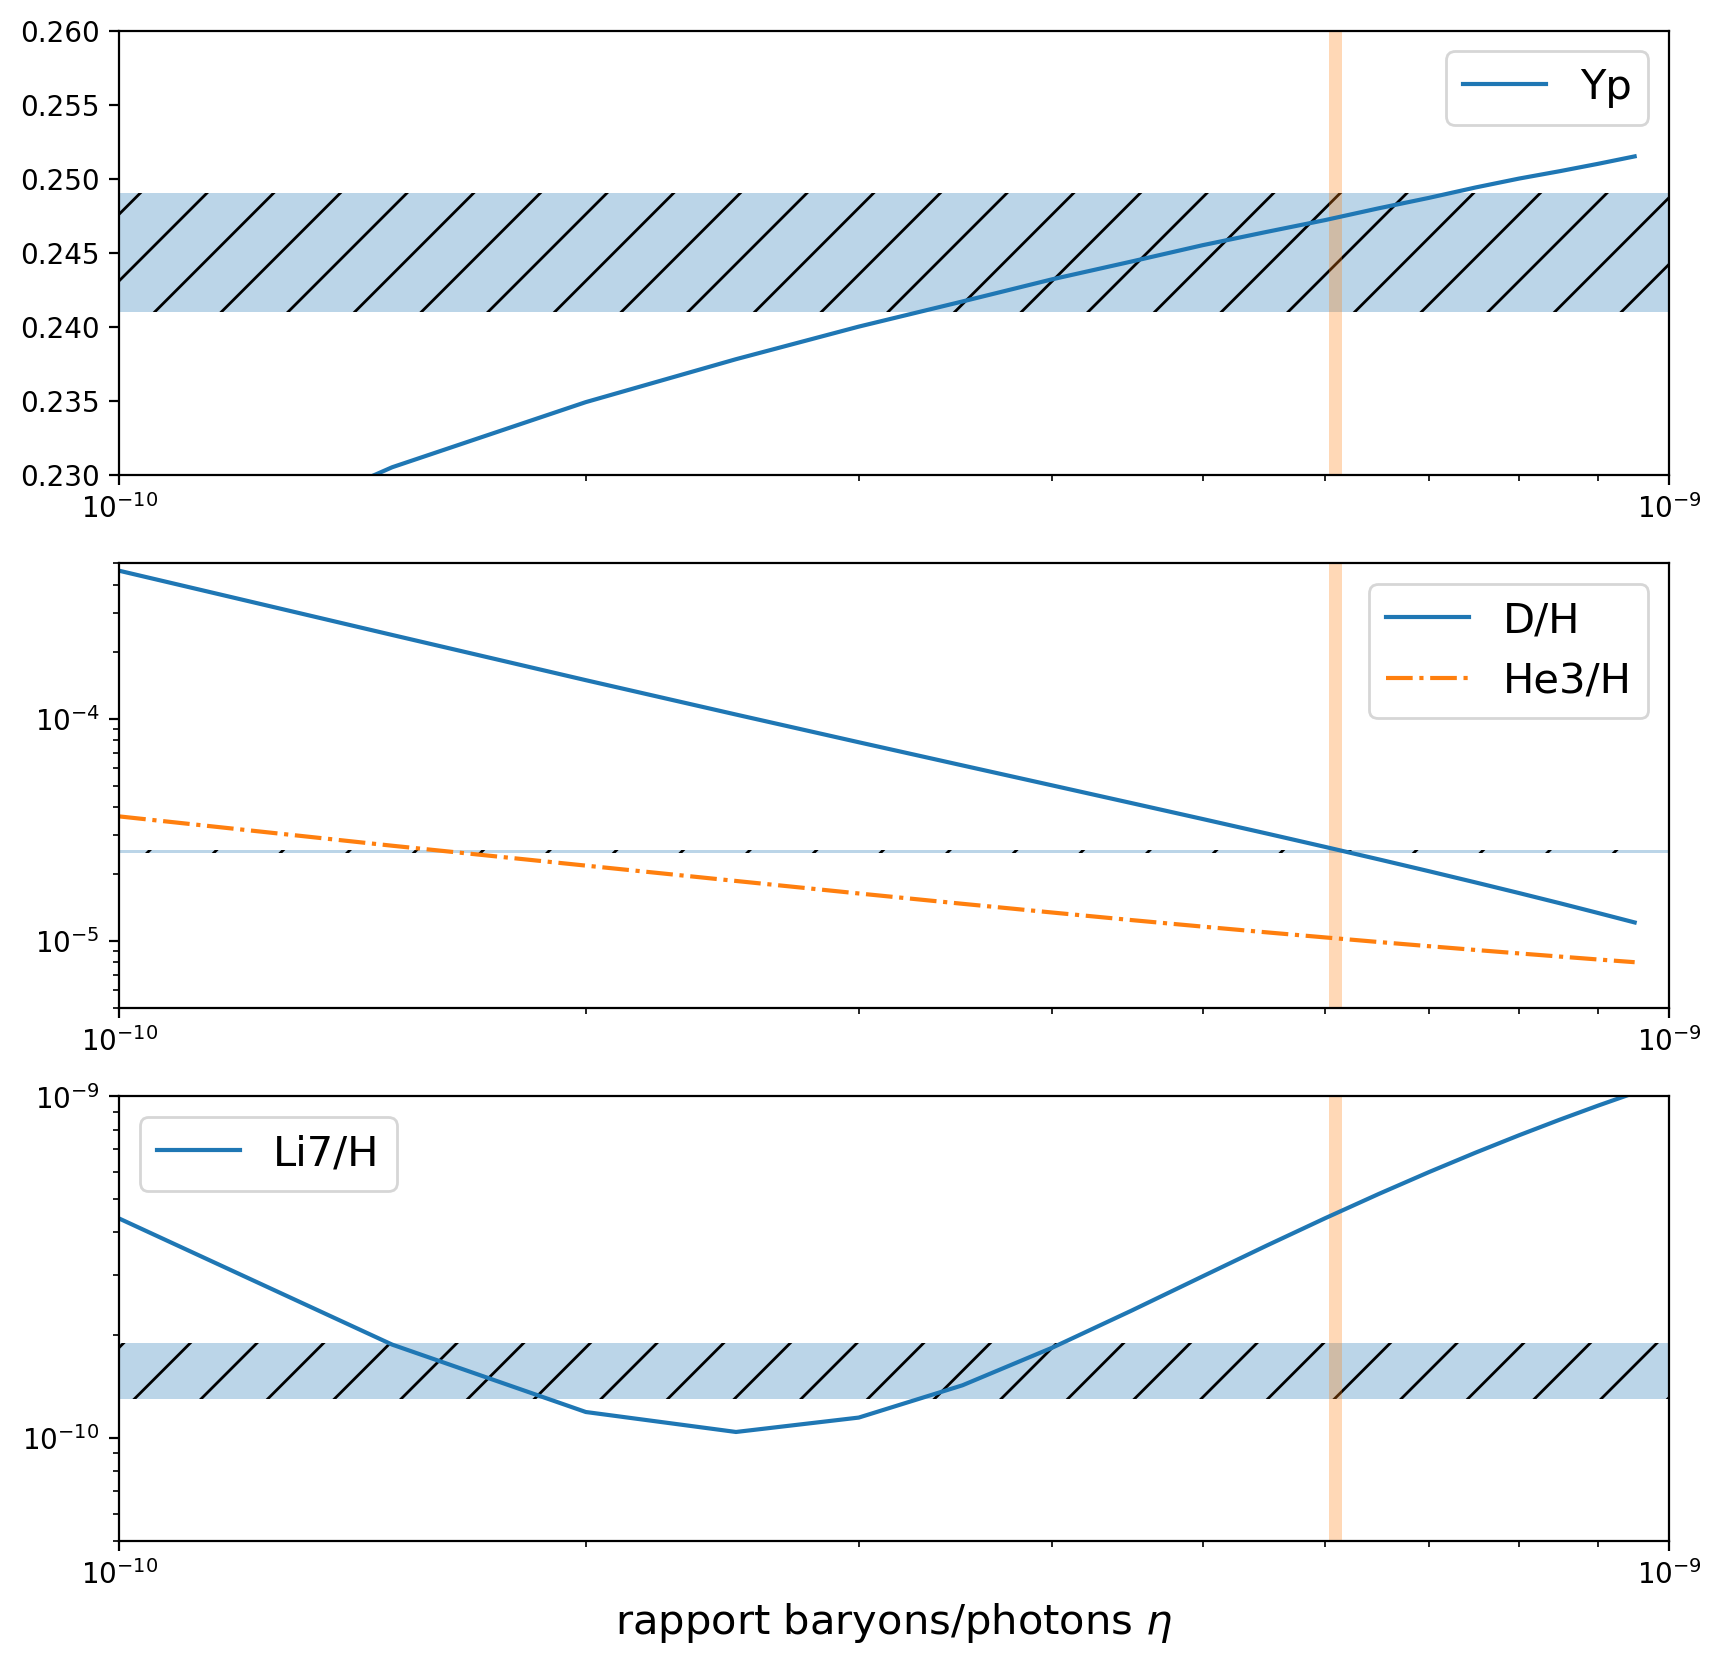
\includegraphics[height=13cm]{figs/BBN.png}
		\caption{Comparaison des abondances observées des éléments légers (régions bleues horizontales, Fields et al. (2015)), des modèles (lignes) et des contraintes Planck (région orange verticale). Ces abondances sont données en fonction du rapport baryon sur photon  $\eta$. Abondances théoriques calculées avec \textit{AlterBBN} (A. Arbey).}
	\label{f:nucle}
\end{figure}

La nucléosynthèse primordiale aboutit à la production de quelques éléments légers, dont en particulier l'hélium. Cette production va dépendre du nombre de baryons à disposition, permettant ainsi de contraindre le paramètre $\Omega_b$ ou de façon équivalente le rapport baryons sur photon $\eta$. La figure \ref{f:nucle} présente la comparaison entre les mesures d'abondances et les modèles de nucléosynthèse primordiale. On constate que pour He$^4$, He$^3$ et D, il y a un régime de concordance pour $\eta \sim 6\times 10^{-10}$ et $\Omega_b h^2\sim 0.022$. L'absence d'accord avec le Lithium s'explique quand à lui par la difficulté d'estimer l'abondance \textit{primordiale} de cet élément, cet élément pouvant être détruit au sein des intérieurs stellaires.

Il est intéressant de constater que ces contraintes sur la quantité de baryons universelle est en accord quasi parfait avec celles issues de l'étude du fond diffus cosmologique (WMAP et Planck). Cet accord est d'autant plus remarquable que ces estimations reposent sur des études très différentes :abondance primordiale d'éléments d'une part, spectre des fluctuations des baryons de l'autre.

Remarquons enfin que les abondances dépendent également de la variation temporelle de la température, régie par l'évolution du facteur d'expansion et donc in fine sur les paramètres cosmologiques. Ainsi les processus de nucléosynthèse se déroule dans une époque où la dynamique de l'Univers est dominée par les espèces relativistes, ainsi dans l'absolu les abondances permettent de contraindre la densité d'énergie des espèce relativistes $\Omega_r$. Par exemple, le nombre d'espèce de neutrinos peut être contraint par cette mesure et les résultats actuels ne permettent pas de dévier du nombre de neutrinos prédit par le modèle standard, à savoir 3.


%%!TEX root = /Users/domaubert/Documents/Lectures/cosmolog/cosmo_main.tex

\chapter{Le Fond Diffus Cosmologique}

Le fond diffus cosmologique constitue la pierre angulaire de la cosmologie actuelle et se présente comme l'un des objets astrophysique le mieux connu et le plus étudié. C'est la conjonction d'une excellente compréhension théorique de cet objet avec l'avalanche de données de grande qualité qui a contribué à installer le fond diffus comme l'un des plus grands succès de la cosmologie.

Le fond diffus cosmologique est communément appelé CMB (pour \textit{cosmic microwave background}) et est constitué des photons "libérés" lors du processus de dernière diffusion. Ce processus a opéré 380 000 ans après le Big Bang et ces photons sont toujours détectable aujourd'hui car présent en grande quantité. Ils sont les reliques d'un époque où l'équilibre matière-rayonnement régnait et présentent une distribution spectrale de corps noir. Ce corps noir possède une température caractéristique d'environ 3K. Il se caractérise également par une intensité sur le ciel qui est uniforme à un très grand niveau de précision. Une étude détaillé de ce rayonnement fait ressortir des fluctuations qui trace la distribution de matière à l'époque de son émission, donnant ainsi accès à une vue sans égal sur le cosmos à ces époques reculées.

\section{Recombinaison}
Si l'on se place après la fin de la nucléosynthèse primordiale ($t>3$ minutes), protons, photons et électrons sont en interaction via 2 types de réactions, la recombinaison et la diffusion Thompson:
\begin{eqnarray}
p + e^- &\leftrightarrow& H+ \gamma\label{e:rec}\\
\gamma +e^- &\leftrightarrow& \gamma +e^- 
\end{eqnarray}
Ces 2 couplages vont disparaître de façon simultanée sous l'effet de la baisse de la densité d'électrons (ou de protons libres) cosmique. On définit la fraction d'ionisation $x$ de la façon suivante:
\begin{equation}
x=\frac{n_p}{n_p+n_H}
\end{equation} 
qui vaut 1 lorsque que le gaz cosmique est complètement ionisé et 0 lorsqu'il est complètement neutre. Notons qu'en raison de la neutralité électrique, la densité de protons libres $n_p$ est égale à la densité d'électrons libres $n_e$. De même, le nombre d'atomes d'hydrogène (crée par l'assemblage d'un proton et d'un électron) est donné par $n_H=(1-x) (n_p+n_H)$. 

L'équation de recombinaison peut être équilibrée via les potentiels chimiques $\mu_p+ \mu_e =\mu_H$ et on rappelle que pour chaque espèce son abondance $n_i$ est donnée par:
\begin{equation}
n_i=g_ie^{\frac{\mu_i}{k_BT}}\left(\frac{m_i k_B T}{2\pi\hbar^2}\right)^{3/2}e^{-\frac{m_i c^2}{k_B T}}.
\end{equation}
On obtient alors l'équation décrivant l'évolution temporelle de la fraction ionisée:
\begin{equation}
\frac{1-x}{x^2}=n_B \frac{g_H}{g_e g_p} \left(\frac{k_B T}{2\pi\hbar^2}\right)^{-3/2} m_e^{-3/2} e^{\frac{\chi}{k_B T}},
\end{equation}
où $n_B=n_p + n_H$ désigne la densité de baryons et $\chi=13.6$ eV est l'énergie de liaison de l'atome d'hydrogène. Notons également que la densité de baryon peut s'écrire en fonction du nombre de photons $n_B=\eta n_\gamma\sim T^3$ et l'équation de l'état d'ionisation peut s'écrire:
\begin{equation}
\frac{1-x}{x^2}=A \eta \left(\frac{k_B T}{m_e c^2}\right)^{3/2}e^{\frac{\chi}{k_B T}}
\label{e:recomb}
\end{equation}
où $A$ est un pré-facteur fonction notamment des facteurs de dégénérescence. Notons que le terme de droite de l'équation \ref{e:recomb} ne dépend que du temps, par conséquent elle se résume à une équation du second degré sur $x$ à un instant donné. On rappelle que cette évolution manifeste \textit{un déplacement de l'équilibre} vers  la droite de l'équation \ref{e:rec}.
\begin{figure}[htbp]
	\centering
		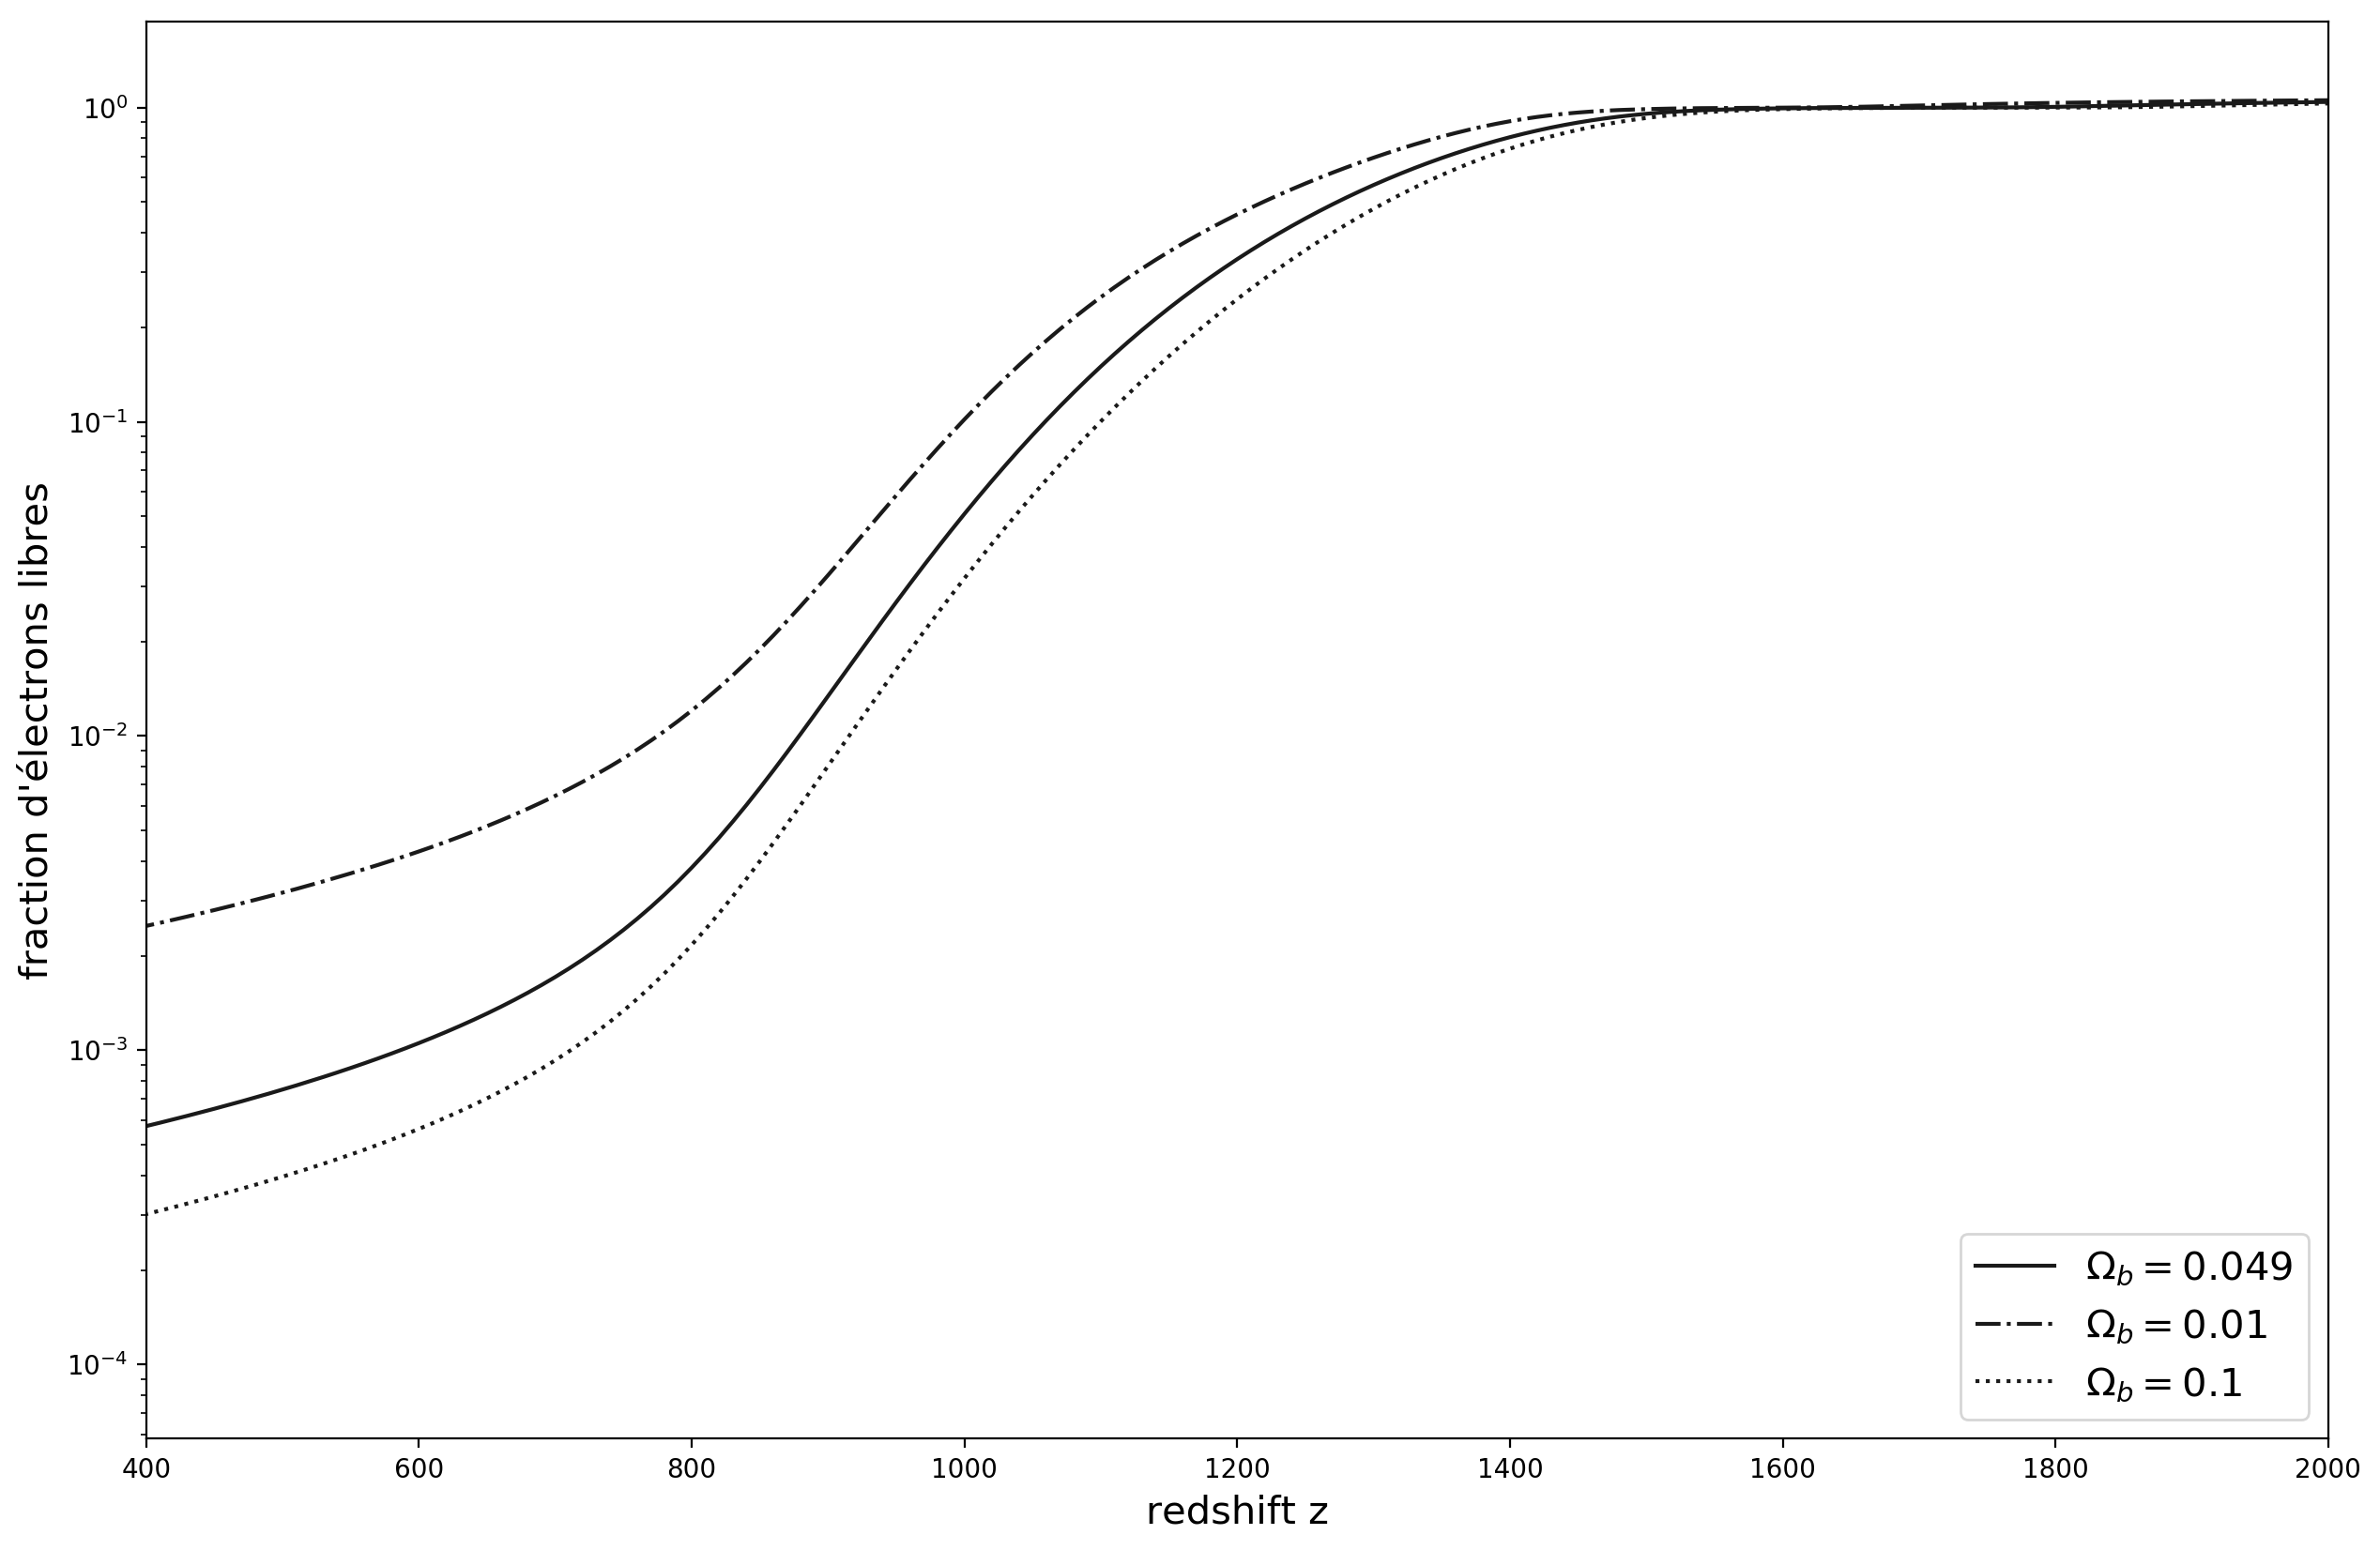
\includegraphics[height=10cm]{figs/recom.png}
		\caption{Evolution temporelle de fraction d'ionisation pour trois valeur de $\Omega_b$.}
	\label{f:recomb}
\end{figure}

La figure \ref{f:recomb} présente l'évolution de la fraction ionisée pour différente valeurs de $\Omega_b$. . Dans tous les cas l'Univers voit la quantité d'atomes ionisés divisée d'un facteur 100-1000 entre z=1500 et z=1000, correspondant à un âge d'Univers t=380 000 ans. On peut constater que ce processus opère plutôt tardivement: l'époque correspondant à l'énergie caractéristique $\chi=$13.6 eV s'est mise en place à $t=180$ ans. De manière analogue au deutérium bottleneck, c'est la grande quantité de photons (par rapport au nombre de baryons) qui empêche une mise en place plus rapide. Si l'on examine la figure \ref{f:recomb} plus en détail on constate d'une part qu'une plus faible densité de baryon ($\Omega_b$ plus faible) conduit à une mise en place moins efficace de la recombinaison. Elle opère plus tardivement et est moins complète dans un Univers moins riche en baryons.

\section{Surface de dernière diffusion}

\paragraph{Fin de la diffusion Thompson} La baisse de la densité électronique qui accompagne la formation d'atomes neutres conduit également à réduire l'efficacité de la diffusion Thompson. Dans un environnement riche en électrons libres, la diffusion force un court libre parcours moyen des photons et empêche le rayonnement de se propager sur de longues distances: c'est la marque d'un Univers opaque, dans lequel l'information ne peut provenir de régions lointaines.  Toutefois lorsque $x\sim 0.01\%$, la diffusion gèle, et se produit alors la \textit{dernière diffusion} à un redshift z=1100. A partir de cet instant, le rayonnement n'interagit plus avec les électrons et de fait se découple de la matière~: ce rayonnement peut dorénavant se propager librement et est détecté aujourd'hui sous la forme du CMB. Notons pour finir que la baisse de la densité électronique va également conduire au gel des réactions de recombinaison vers z=1100, avec un ionisation résiduelle de l'ordre de 0.01\%.



\paragraph{surface de dernière diffusion}

\begin{figure}[htbp]
	\centering
		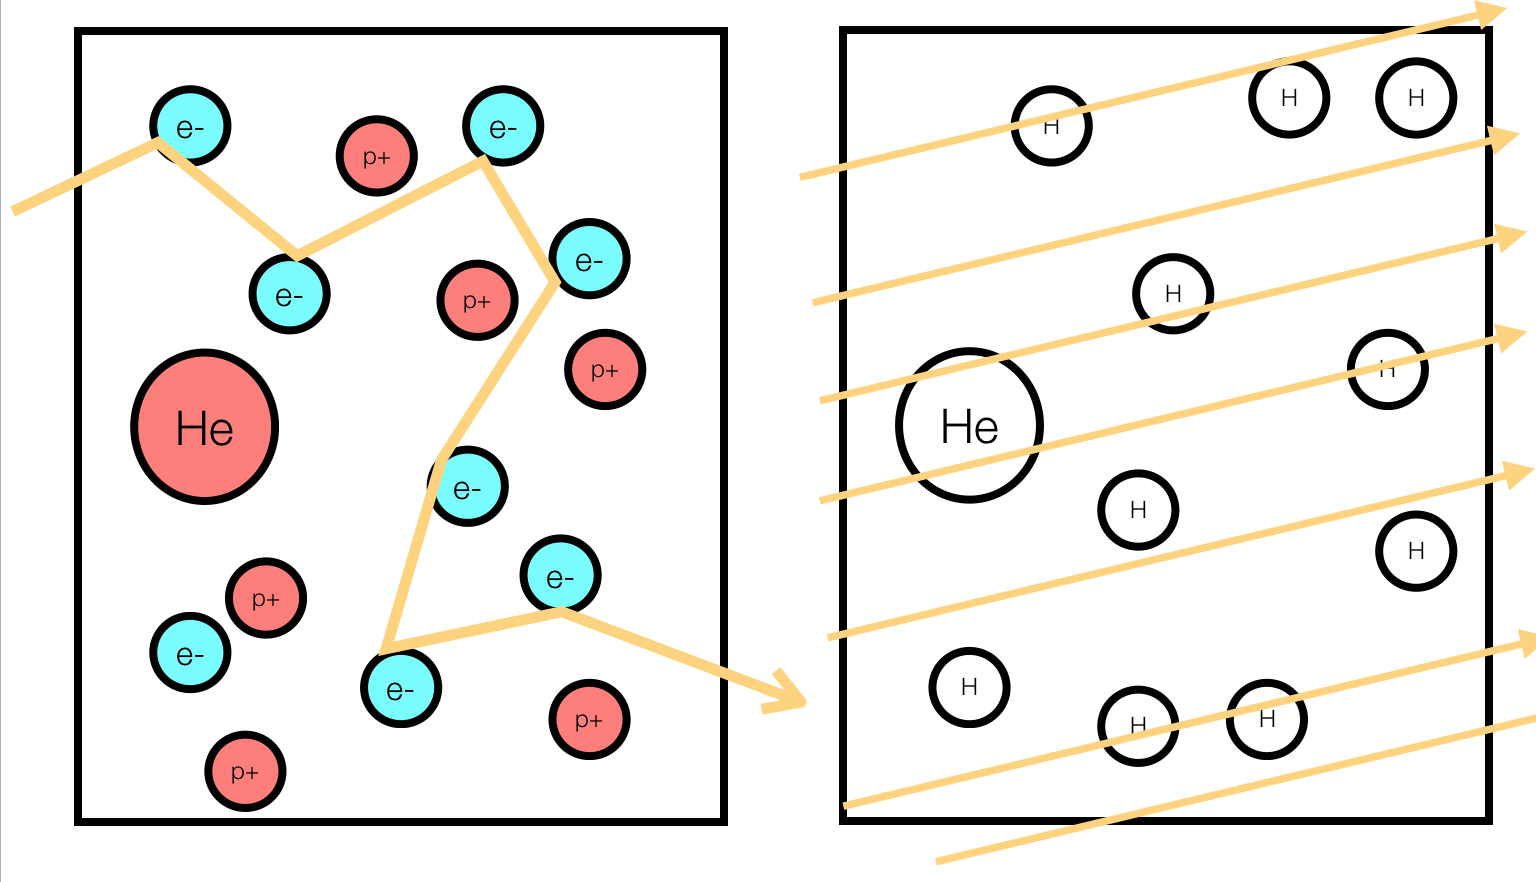
\includegraphics[height=12cm]{figs/diffusion.png}
	\caption{Avant la recombinaison, la présence d'électrons libres dans le plasma cosmique est à l'origine d'un processus de diffusion des photons important. Le plasma peut alors être considéré comme opaque, compte tenu de l'impossibilité d'extraire de l'information sur des grandes distances. La seule information disponible provient de la dernière diffusion. Après la recombinaison, l'absence d'électrons libres permet enfin au rayonnement de se propager librement, l'Univers devient transparent pour les photons du fond diffus cosmologique.}
	\label{f:diffusion}
\end{figure}

A partir de $z=1100$ les photons du fond diffus vont pouvoir se propager librement et de façon essentiellement rectiligne. Les photons du fond diffus qui nous parviennent aujourd'hui sont donc issus de toutes les régions du celle distantes de telle manière à ce que le rayonnement mette 13.8 milliards d'années à nous parvenir. L'ensemble de ces régions définit une coquille, centrée sur l'observateur et de distance de parcours lumineux égale à l'âge de l'Univers. Cette coquille possède une faible épaisseur, correspondant à la durée qu'aura mis la diffusion Thompson à geler, comparable à la durée qu'à mis la recombinaison à se mettre en place ($\Delta z\sim 100$). Vu depuis l'observateur, cette coquille apparaît donc comme une surface sphérique vue depuis l'intérieur, \textit{la surface de dernière diffusion}. Les régions au delà de cette surface de dernière diffusion nous sont inaccessibles par l'intermédiaire des photons, puisque ces derniers n'emporte que l'information de la dernière diffusion~: les régions au delà de cette sphère sont opaques à toute observation et les régions en deçà (à l'intérieur) de cette sphère constitue l'Univers observable de l'observateur placé en son centre.

\begin{figure}[htbp]
	\centering
		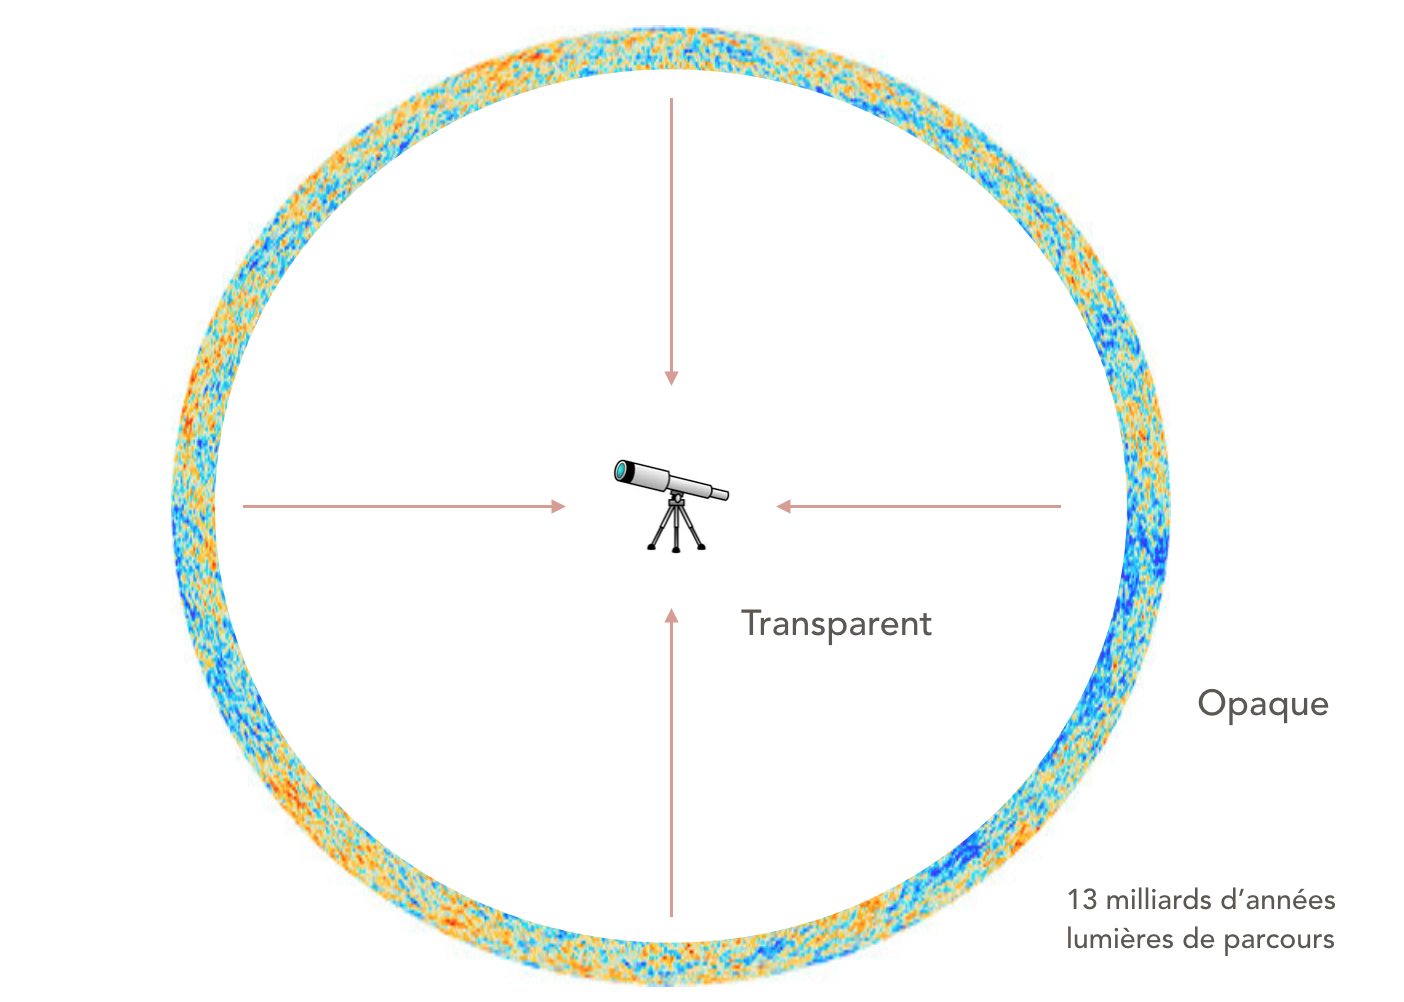
\includegraphics[height=12cm]{figs/LSS.png}
	\caption{Les photons du fond diffus ont pu se propager librement à partir du même instant, correspondant à un Univers âgé de 380 000 ans. Un même instant correspond à une même distance : tous les photons reçus aujourd'hui proviennent de régions situées sur une surface sphérique, dont nous sommes le centre. Son rayon est tel que le parcours des photons est d'environ 13 milliards d'années de vol. Les régions plus distantes que cette 'surface de dernière diffusion' sont opaques, celle moins distantes sont transparentes à ce rayonnement.}
	\label{f:LSS}
\end{figure}

Rappelons que ces photons sont ultra-dominant en nombre, avec par exemple un rapport baryon/photon $\eta\sim6e-10$. Cela a plusieurs conséquences: d'une part cela signifie qu'aucun processus astrophysique n'est en mesure de faire disparaître ce rayonnement et il est de fait toujours mesurable aujourd'hui. D'autre part cette domination est telle que l'impression même de signatures de processus astrophysique entre z=1100 et aujourd'hui ne peut se faire qu'à des niveaux très faible. Par conséquent ce rayonnement possède toujours un spectre de corps noir (décalé vers le rouge) même si il n'est plus en situation d'équilibre avec la matière. De même les éventuelles marques des propriétés de l'Univers âgé de 380 000 ans s'y trouve toujours. L'observation de la surface de dernière diffusion est donc une fenêtre incomparable sur l'état du cosmos à ces époques lointaines.




\section{Corps noir cosmologique}
Le fond diffus cosmologique est issu d'une époque où matière et rayonnement étaient couplés et par conséquent possédait à ces époques reculées un spectre de corps noir. La densité volumique de photons dans l'intervalle $[\nu,\nu+d\nu]$ est donné par:
\begin{equation}
n(\nu)d\nu=\frac{8\pi}{c^3}\frac{\nu^2d\nu}{e^{h\nu/k_BT}-1}.
\end{equation}
Comme indiqué précédemment, la surabondance de ces photons est telle que ce signal a conservé les caractéristique d'un tel corps noir, même dans un régime de faible couplage entre matière et rayonnement. Aujourd'hui la température de ce 'corps noir' est mesurée avec une très grande précision (voir aussi la figure \ref{f:bb}):
\begin{equation}
T_0=2.7255\pm0.0006 K.
\end{equation}
\begin{figure}[htbp]
	\centering
		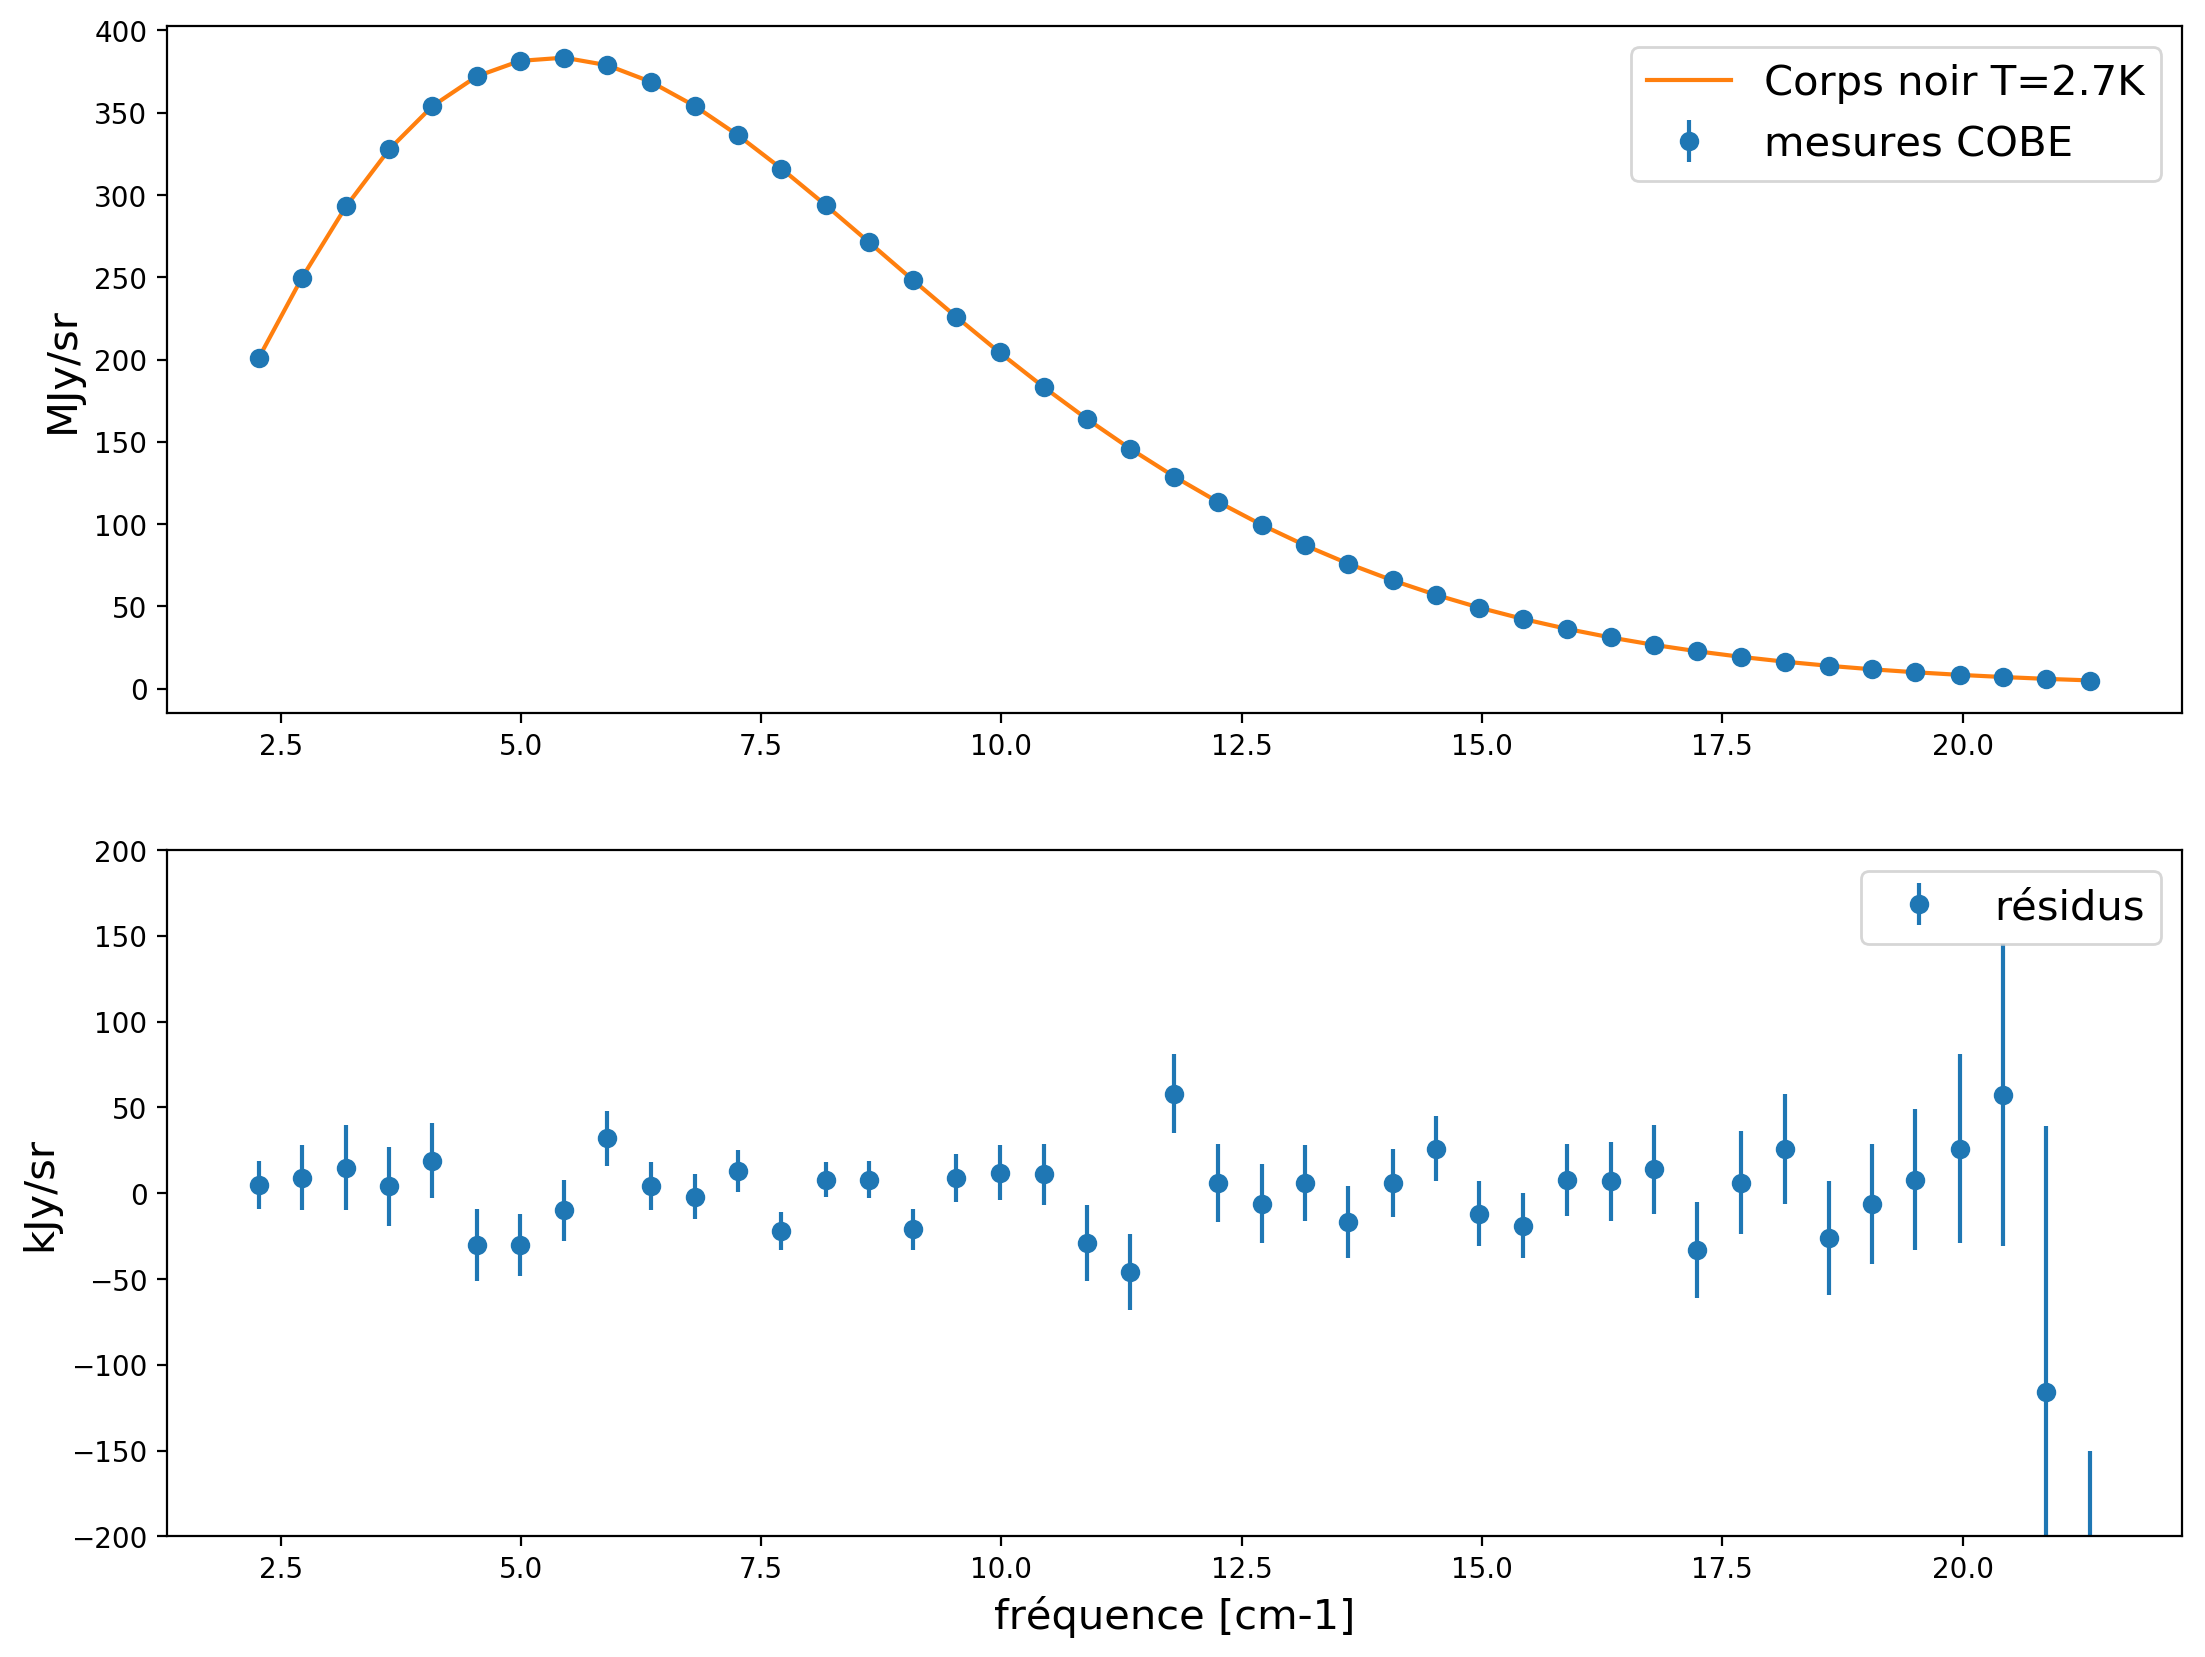
\includegraphics[height=10cm]{figs/bb.png}
		\caption{Le spectre du fond diffus cosmologique: les symboles représentent les mesures de l'instrument FIRAS, la ligne le spectre de corps noir pour une température de $T_0=2.725$K. Figure extraite de Fixsen 2009.}
	\label{f:bb}
\end{figure}
Ce spectre va conserver sa forme, malgré le redshift des photons concernés et malgré la modification de leurs fréquences selon:
\begin{equation}
\nu(a)=\frac{\nu_0}{a}.
\end{equation}
Dans un volume de contrôle de volume $V=V_0a^3$ et dans un intervalle de fréquence $d\nu=d\nu_0/a$, le nombre de photon doit rester identique quel que soit l'instant considéré:
\begin{equation}
\frac{\nu^2d\nu}{e^{h\nu/k_BT}-1}V=\frac{\nu_0^2d\nu_0}{e^{h\nu_0/k_BT_0}-1}V_0,
\end{equation}
qui ne peut être satisfait que si la température caractéristique du corps noir suit la relation :
\begin{equation}
T=\frac{T_0}{a}=T_0(1+z)
\end{equation}
que nous avions déjà établi. On remarque ainsi que la recombinaison opérant à $z\sim1100$, la température du gaz de photon cosmique était proche des 3300 K.

\section{Anisotropies du CMB}
Le fond diffus est représentatif d'un Univers jeune (t=380 000 ans) et donc très proche de l'homogénéité parfaite. Par conséquent sa mesure fait apparaître une très grande stabilité du signal sur tout le ciel, sans fluctuations de température détectable jusqu'à des niveaux de 0.001 K. Au delà, commence toutefois à apparaître des anisotropies dans le signal~: celles-ci sont essentiellement générées par la physique des baryons à l'œuvre au moment de la recombinaison et par des processus astrophysiques qui affecte le rayonnement au cours de son vol jusqu'à l'observateur. L'étude de ces anisotropies est extrêmement riche d'informations pour la physique fondamentale, la cosmologie et l'astrophysique. Notons que nous allons nous concentrer sur les fluctuations de température et implicitement le mot "fluctuation" ou "signal" désigne ce type de donnée. Il existe également des études en \textit{polarisation} que nous n'aborderons que très rapidement en fin de chapitre.

\begin{figure}[htbp]
	\centering
		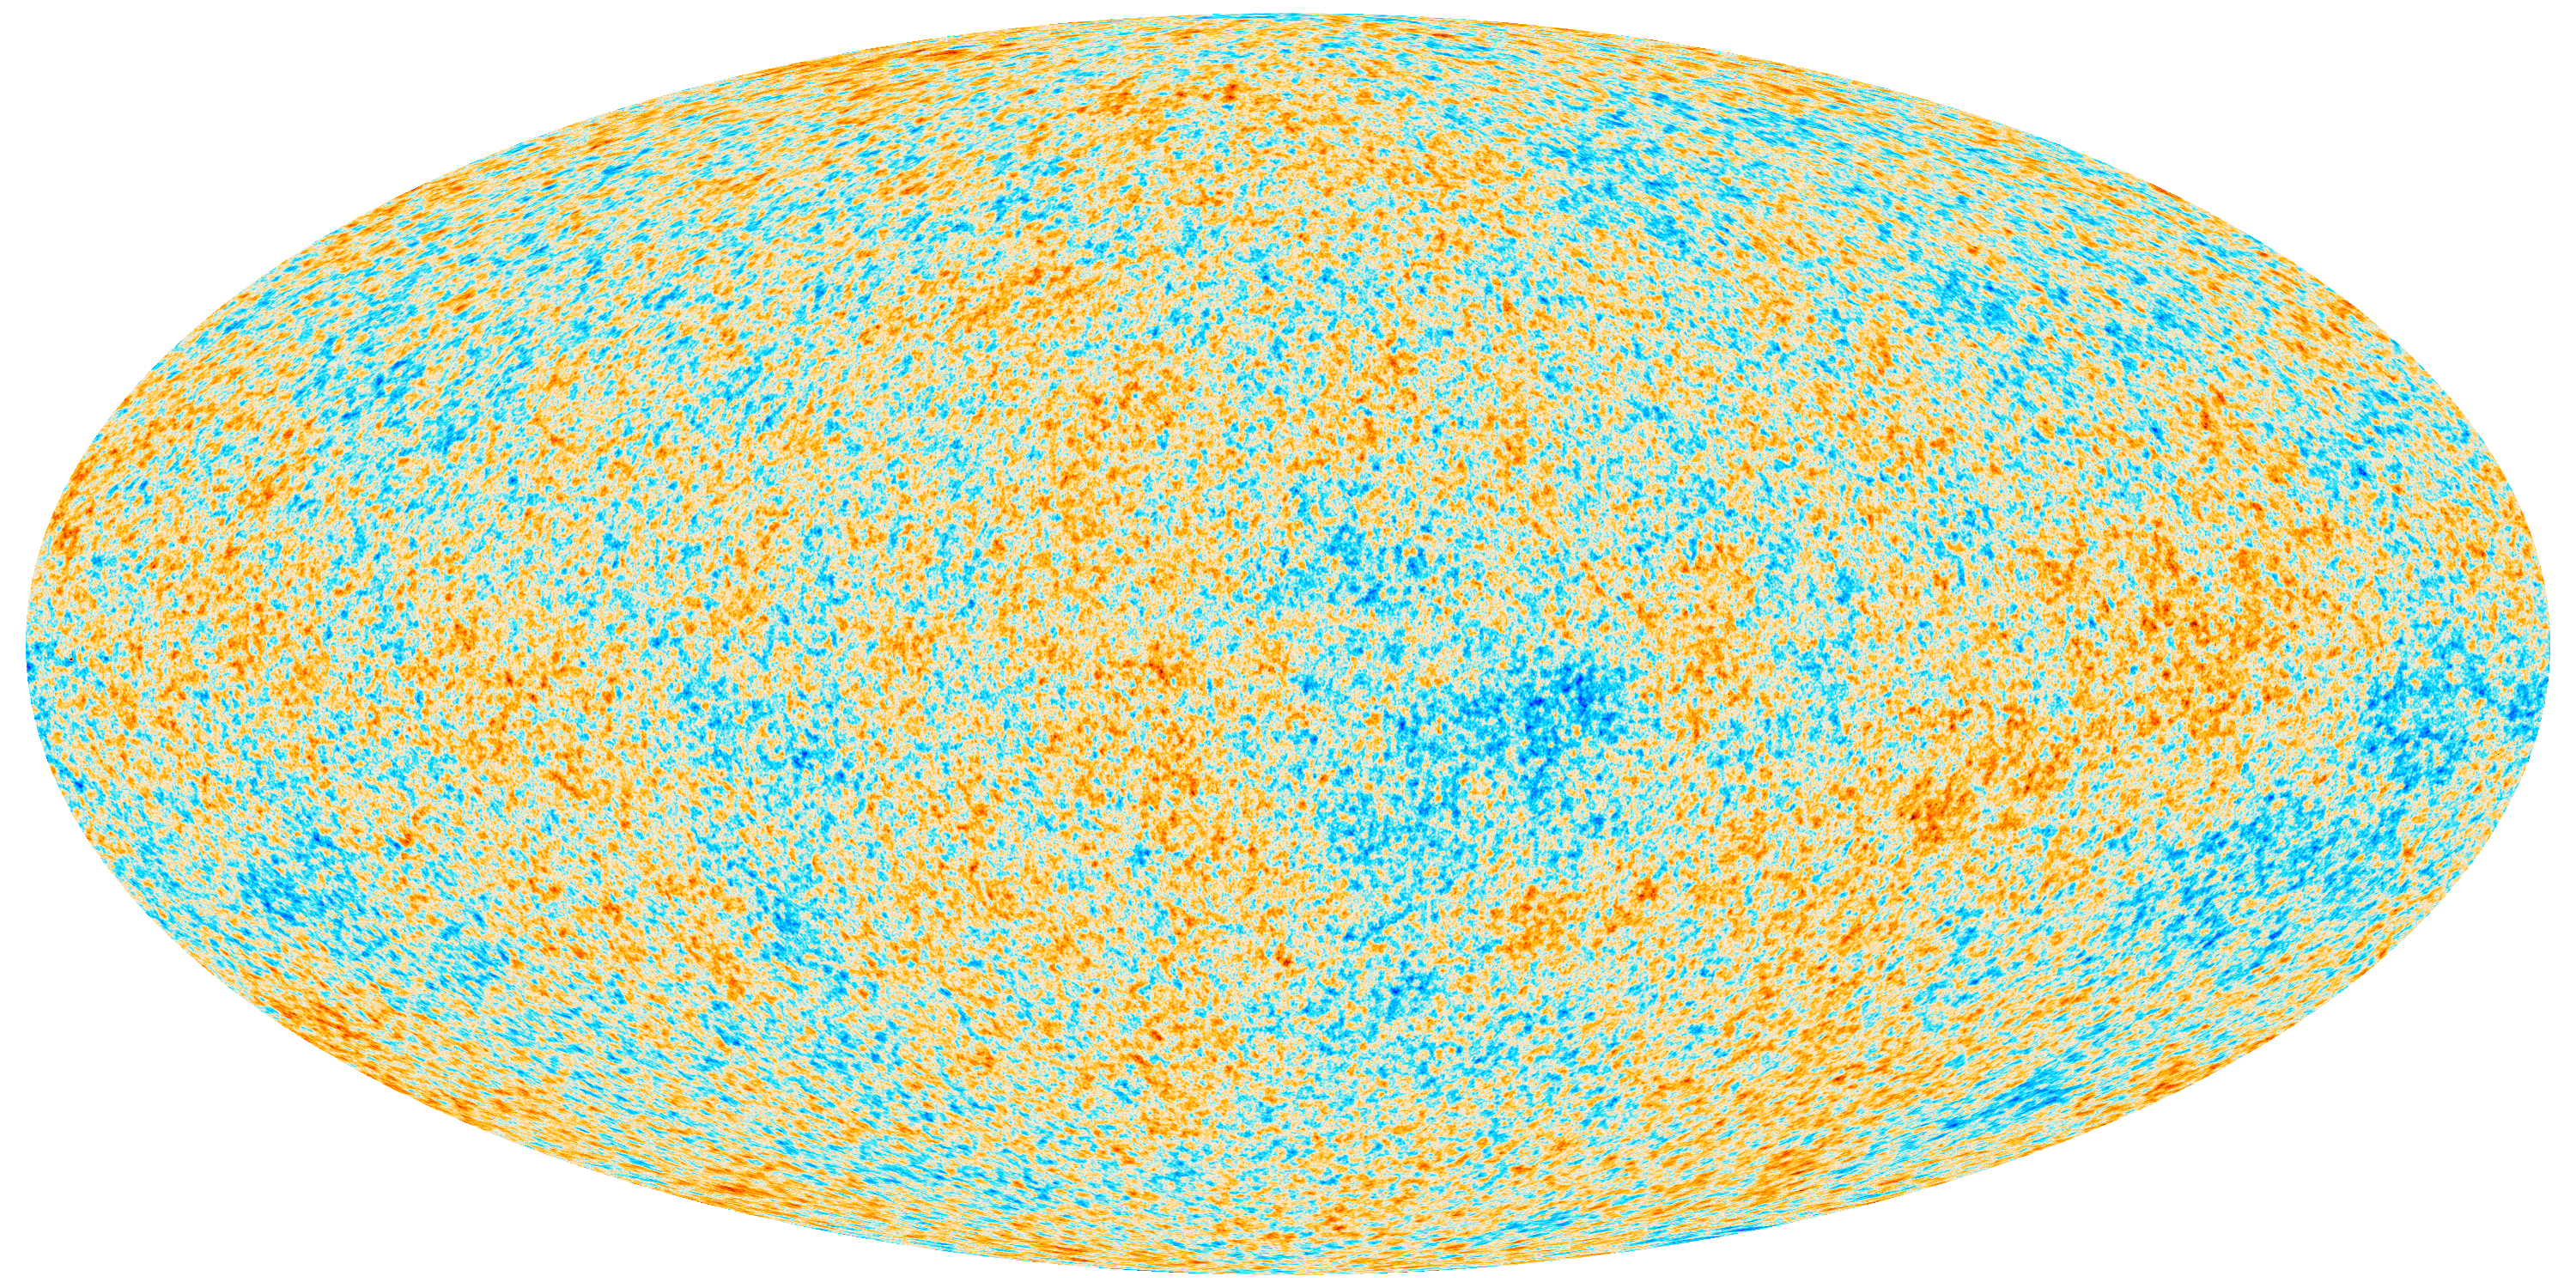
\includegraphics[height=6cm]{figs/planck2015.png}
		\caption{La carte des anisotropies du fond diffus obtenue par la mission européenne \textit{Planck}. Les zones jaunes sont plus chaudes que les zones bleues. Le niveau des fluctuations représentées est de l'ordre de 0.001\%.}
	\label{f:planckmap}
\end{figure}

\subsection{Principe de l'analyse des anisotropies du CMB}
Dans cette section, nous allons exposer rapidement les grands principes de l'analyse du signal du fond diffus. Le CMB se manifeste pour l'observateur comme un signal sur tout le ciel, généralement sous la forme d'une carte de température $\delta T(\theta,\phi)$, mesurée dans un repère sphérique. Afin de pouvoir extraire de l'information de ce type de données, l'on raisonne généralement sur la transformée de Fourier de ce signal. Cette opération permet d'une part de séparer les contributions des différentes échelles angulaires. D'autre part, nous verrons que la théorie qui permet de prédire les propriétés de ces fluctuations se fait naturellement dans l'espace de Fourier, où les différentes échelles angulaires évoluent de façon découplées en très bonne approximation.  Dans un espace sphérique, les opérations de transformées de Fourier s'effectue via la base des harmoniques sphériques $Y_{\ell,m}(\theta,\phi)$ et la carte de températures se décompose de la façon suivante:
\begin{equation}
\delta T(\theta,\phi)= \sum_{\ell=0}^{\infty}\sum_{m=-\ell}^{\ell} a_{\ell,m} Y_{\ell,m}(\theta,\phi),
\end{equation}
où les coefficients (complexes) $a_{\ell,m}$ sont obtenus par projection de la carte sur la base vectorielle composée des harmoniques:
\begin{equation}
a_{\ell,m}=\int \int d\theta d\phi\sin \theta Y^*_{\ell,m}(\theta,\phi) \delta T(\theta,\phi).
\end{equation}
Les coefficients $a_{\ell,m}$ constituent ainsi la contribution de chaque harmonique à la carte de température.

\paragraph{Echelles angulaires}
 Les harmoniques sphériques sont les analogues des modes de Fourier sur la sphère, à savoir une base de sinus et cosinus adapté à une géométrie sphérique. Le coefficient $\ell$ trace l'échelle angulaire de l'harmonique qui possède ainsi une taille angulaire caractéristique $\theta\sim\pi/\ell$: on parle également de fréquence angulaire où les bas $\ell$ désigne les grandes échelles sur le ciel et les grands $\ell$ les petites échelles. Le coefficient $m$ peut varier entre $-\ell$ et $\ell$ et désigne les différentes orientations indépendantes pour chaque taille angulaire caractéristique: celle ci sont d'autant plus nombreuses que la fréquence angulaire est élevée. L'harmonique $\ell=0$ correspond au monopole, à savoir un signal uniforme sur toute la sphère et dont le coefficient $a_{00}$ renvoie directement à la moyenne sur tout le ciel. Les harmoniques $\ell=1$ sont des dipôles, avec un côté 'chaud' et un côté 'froid' diamétralement opposés.

\paragraph{Spectre de puissance}
\begin{figure}[htbp]
	\centering
		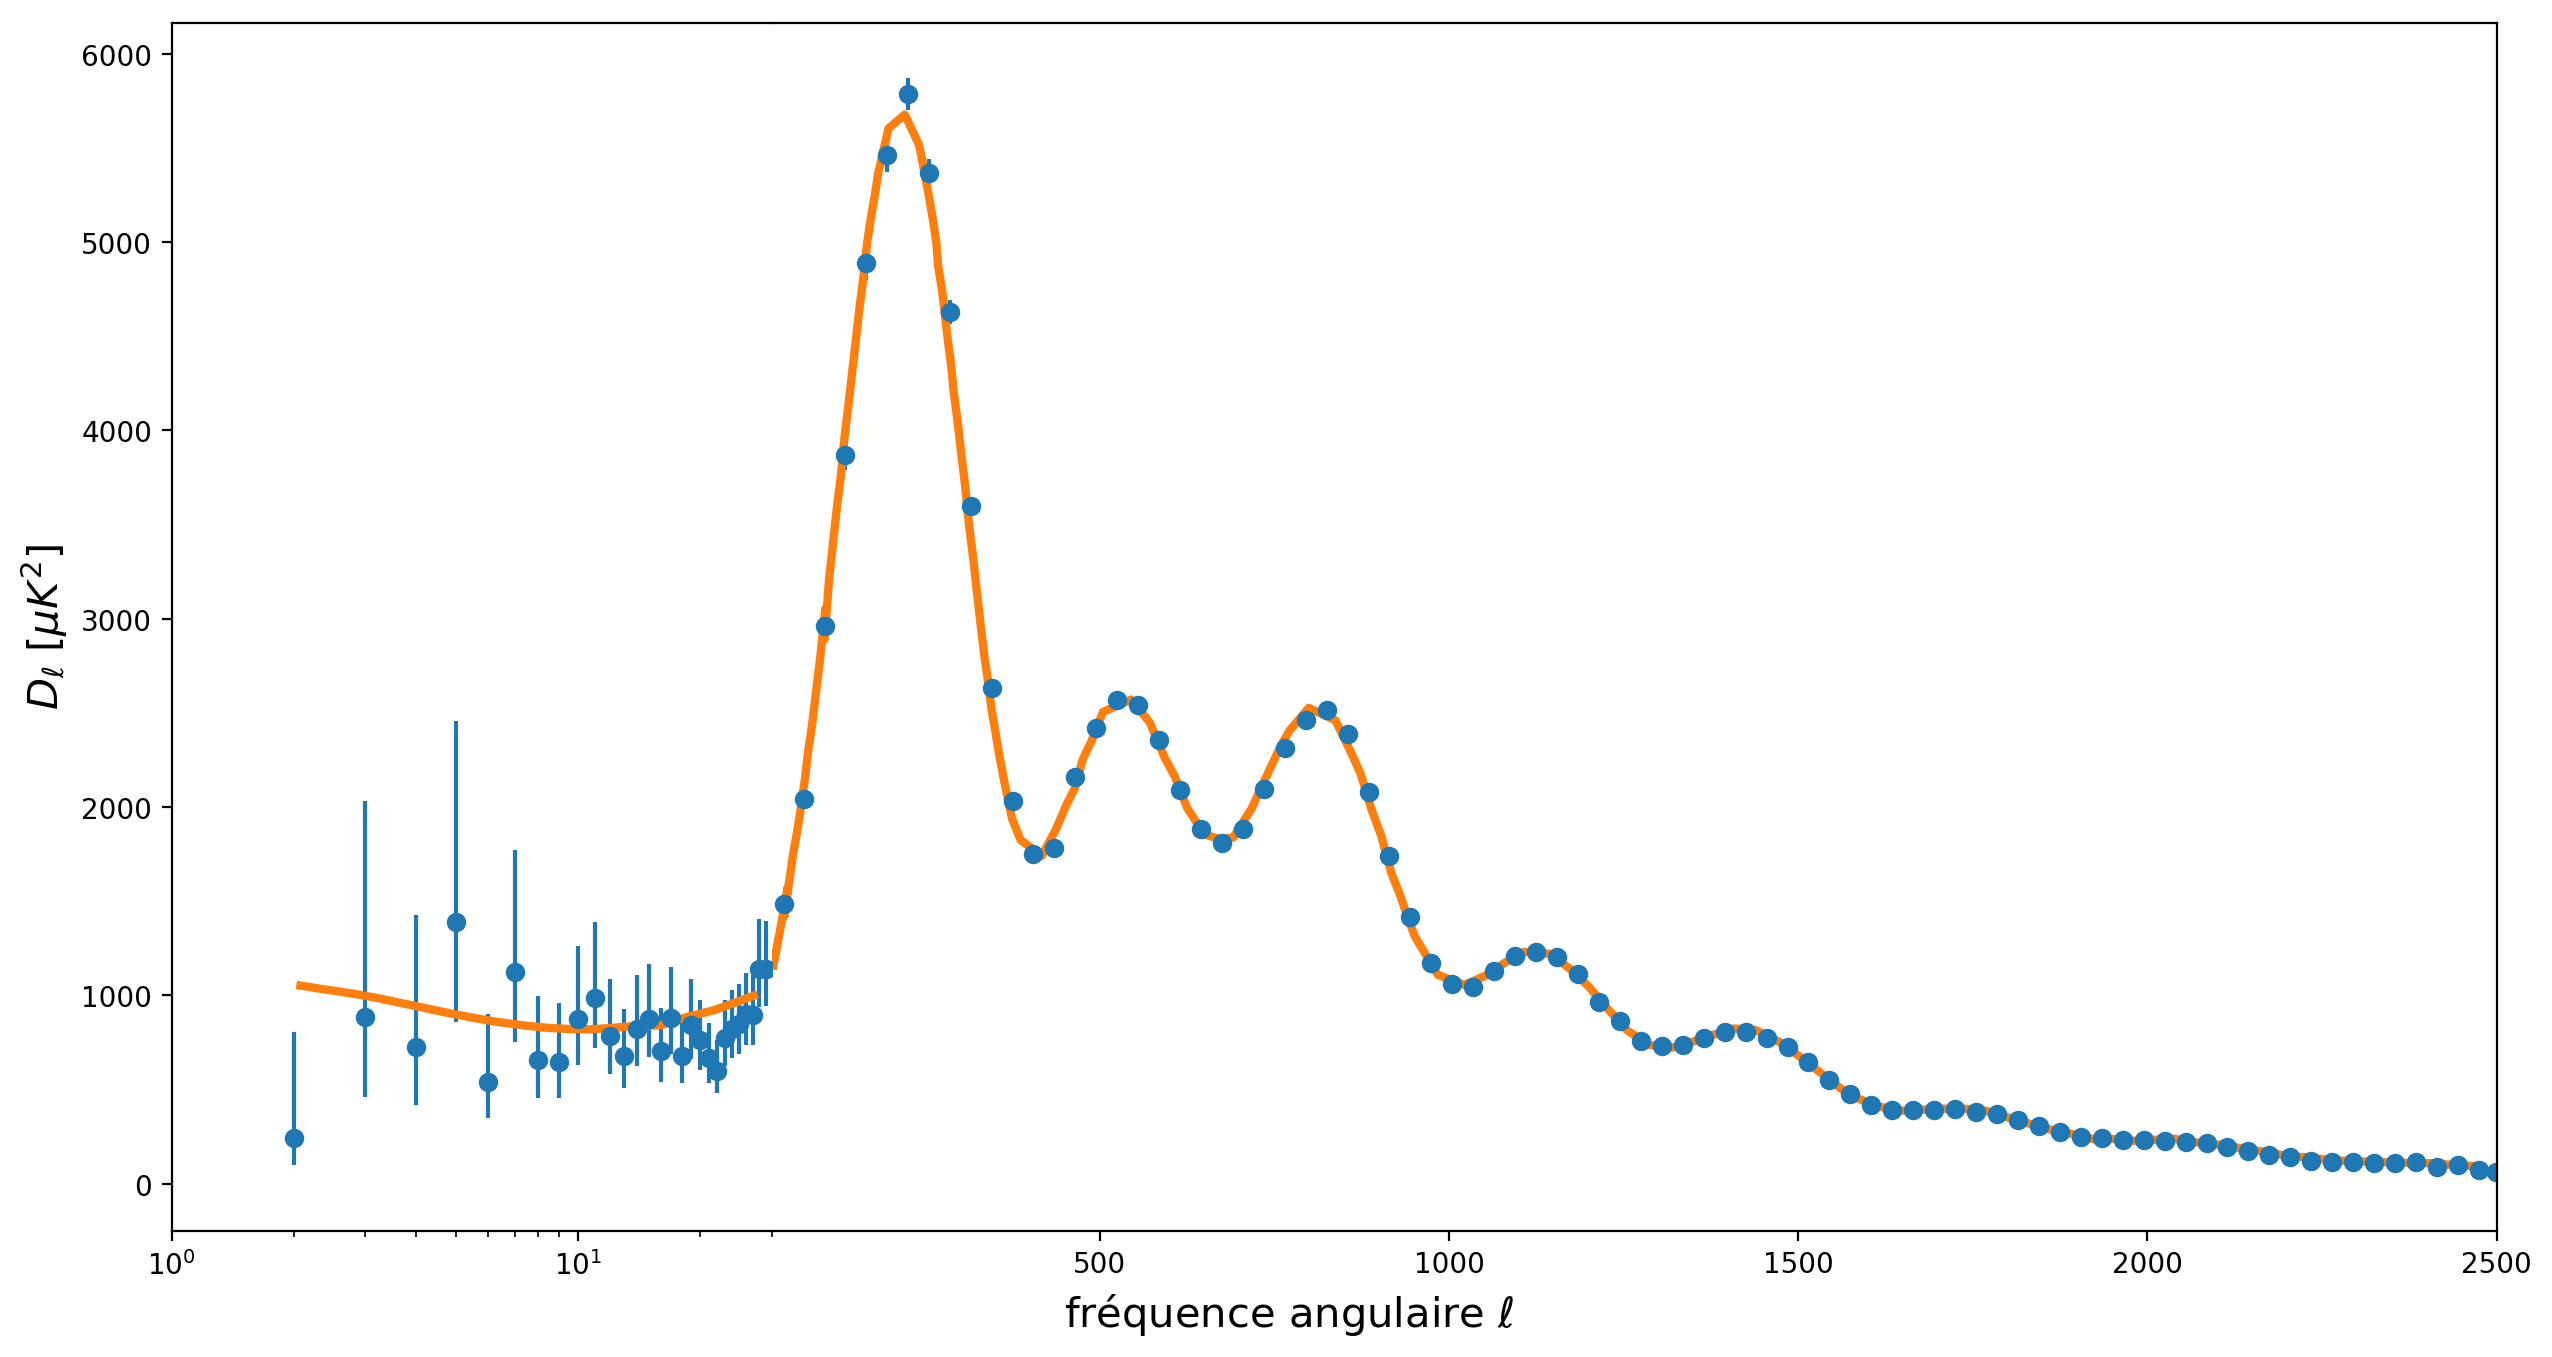
\includegraphics[height=8cm]{figs/cl2015.png}
		\caption{Le spectre de puissance des anisotropies du fond diffus cosmologique obtenu par \textit{Planck}. Le panneau supérieur représente $D_\ell=\ell(\ell+1)C_\ell$~: les points sont les données et la ligne représente le spectre prévu pour un modèle $\Lambda$CDM. Le panneau inférieur montre les résidus entre le modèle et les points de données.}
	\label{f:cl}
\end{figure}

Armé de la collection des coefficients $a_{\ell,m}$ d'une carte du ciel, on évalue les contributions relatives de chaque échelle par le spectre de puissance angulaire:
\begin{equation}
C_\ell=\langle |a_{\ell,m}|^2\rangle=\frac{1}{2\ell+1}\sum_{m=-\ell}^{\ell} |a_{\ell,m}|^2
\end{equation}
Ce faisant, on rassemble pour chaque échelle angulaire $\ell$ les contributions de toutes les orientations $m$ associées. Si toutes les directions sont à priori équivalentes et aucune n'est privilégiée, alors cette opération ne produit pas de perte d'information. C'est le cas du CMB, celui-ci étant à priori isotrope. D'autre part, une grande classe de modèles d'inflation prédisent que les fluctuations du fond diffus doivent appartenir à la classe des \textit{champs aléatoires gaussiens} qui sont entièrement définis par leur 'variance', ce qui est précisément la nature du spectre de puissance angulaire.

\subsection{Avant-plans}

Avant toute chose, il est important de réaliser qu'une carte brute du ciel aux longueurs d'ondes sondées par les missions CMB est soumise à une forte contamination par des avant-plans astrophysiques. Parmi ces avant-plans, le plus spectaculaire est sans contexte la Galaxie dont par exemple l'émission  par les poussières ou le rayonnement synchrotron empêchent d'accéder aux fluctuations du CMB en arrière plan. Ces avant-plans peuvent être ajustés, modélisés et pris en compte dans des modèles d'inversion, afin d'extraire le signal d'origine cosmologique des portions du ciel affectées. Notez que ces avant-plans sont également source de recherches dédiées, notamment à propos des propriétés des poussières dans la Voie Lactée.

\paragraph{Dipôle} Le premier niveau d'anisotropie est constitué par le dipôle du CMB. Il possède une amplitude de l'ordre de 3 mK et résulte du mouvement de l'observateur par rapport à la surface de dernière diffusion. Ce mouvement induit un effet Doppler, fonction de la vitesse de déplacement et qui fait apparaître des zones plus chaudes et plus froides que la moyenne, diamétralement opposées et alignées avec la direction de déplacement. Au premier ordre, la variation de température dans la direction du dipôle obéit à la relation:
\begin{equation}
\left(\frac{\Delta T}{T}\right)_\mathrm{dipole}\sim \frac{v}{c}
\end{equation}
et donne une valeur de vitesse de déplacement $v\sim 330$ km/s pour le barycentre du système solaire. Cette vitesse est la somme notamment de la vitesse de déplacement du Soleil dans la Galaxie et de la Galaxie dans le Groupe Local.

\subsection{Anisotropies Intrinsèques}
Les fluctuations de température du CMB tracent des fluctuations de densité de matière. Plusieurs modèles de couplage entre matière et rayonnement existent, mais un grand nombre d'évidences observationnelles pointent vers des fluctuations de type \textit{adiabatiques}. Dans ce mode de couplage, le rapport entre la densité de matière et celle de rayonnement reste constant y compris au sein des fluctuations locales : le fluide de matière ne dérive pas par rapport au fluide de photons. Dans ce cas le rapport des densités reste constant:
\begin{equation}
\frac{n}{n_\gamma}=\mathrm{cste}\rightarrow\frac{\delta n}{n}=\frac{\delta n_\gamma}{n_\gamma}
\end{equation}
Pour la matière, densité de matière et d'énergie sont directement reliées $\epsilon=n m c^2$ et
\begin{equation}
\frac{\delta n}{n}=\frac{\delta \epsilon}{\epsilon}.
\end{equation}
Pour les photons, nous avons déjà vu que $n_\gamma \sim T^3$ :
\begin{equation}
\frac{\delta n_\gamma}{n_\gamma}=3 \frac{\delta T}{T}.
\end{equation}
D'où il apparaît que les fluctuations de températures tracent les fluctuations de densité via:
\begin{equation}
\left(\frac{\delta T}{T}\right)_\mathrm{adiab}=\frac{1}{3}\frac{\delta n}{n}=\frac{1}{3}\frac{\delta \rho}{\rho}.
\end{equation}
Dans un régime de fluctuations adiabatiques, les régions plus chaudes (respectivement plus froides) que la moyenne correspondent aux régions les plus dense au même moment. 

Toutefois les fluctuations de densité produisent également des fluctuations de potentiel gravitationnel qui devront être gravie ou dévalées par les photons du fond diffus au moment de leur émission. Les photons en train de sortir d'un puit (correspondant à une surdensité) seront décalées vers le rouge (perte d'énergie) et ceux en train de dévaler un pic de potentiel (correspondant à une sous densité seront décalés vers le bleu (gain d'énergie). Cet effet se nomme \textit{effet Sachs-Wolf}:
\begin{equation}
\left(\frac{\delta T}{T}\right)_\mathrm{SW}=-\delta\phi
\end{equation}
où $\delta \phi$ est la fluctuation de potentiel. Par ailleurs on peut montrer que la variation de potentiel est liée à la fluctuation de densité via $\delta \rho/\rho=2\delta \phi$ ce qui implique que la variation de température \textit{totale} est donnée par :
\begin{equation}
\left(\frac{\delta T}{T}\right)_\mathrm{total}=\left(\frac{\delta T}{T}\right)_\mathrm{SW}+\left(\frac{\delta T}{T}\right)_\mathrm{adiab}=-\frac{1}{3}\delta \phi=-\frac{1}{6}\frac{\delta \rho}{\rho}
\end{equation}
Les points chaud du CMB correspondent à des régions sous-dense de l'Univers au moment de l'émission. La carte de température du CMB est donc une carte de la distribution de matière au même instant. Ces fluctuations se situent à des niveaux de 0.001\%, indiquant par la même que l'Univers était extrêmement homogène au moment de la recombinaison.

\paragraph{Grandes échelles} Reste à expliciter l'origine des fluctuations de densité qui conduisent aux fluctuations de températures. L'examen de la figure \ref{f:cl} permet de distinguer 2 régimes. Le premier régime correspond aux grandes échelles $\ell<30$: ces modes sont plus grands que l'Horizon au moment de la recombinaison et tracent les fluctuations les plus primordiales, dont on pense qu'elles sont issues d'une période inflationnaire présente aux tous premiers instants après le Big-Bang. L'étude de ces régions du spectre permet notamment de mesurer l'amplitude des fluctuations inflationnaire ainsi que le spectre de ces fluctuations. En particulier, les théories inflationnaires indiquent que le spectre de puissance tridimensionnel des fluctuations primordiales doit être invariant d'échelle et de la forme:
\begin{equation}
P(k)\sim k^{n_s}
\end{equation}
avec $n_s$ proche mais différent de 1. Les résultats de \textit{Planck 2015} indiquent que $n_s=0.968\pm0.006$ en accord avec ces théories.

\paragraph{Petites échelles} Au delà de $\ell\sim 30$, le spectre présente un ensemble de modes correspondant à des échelles caractéristiques et qui se manifestent sous forme de pics: on en dénombre 3 principaux suivis d'environs 6 pics d'amplitude décroissante. Ces pics indiquent l'existence d'échelles privilégiées dans la carte des fluctuations: ces échelles résultent d'ondes sonores se propageant dans le plasma au moment de la recombinaison. Ces ondes sonores sont appelées \textit{oscillations baryoniques acoustiques} (BAO en anglais) : leur production sera décrite en détail dans le chapitre dédié à la croissance des grandes structures. Ces oscillations se mettent en place pour des échelles sub-horizon d'où leur présence seulement aux petites échelles: la position du premier pic permet ainsi de tracer la taille sur le ciel de l'horizon sonore. Connaissant la taille \textit{intrinsèque} de cet horizon, la mesure de la taille apparente permet de déduire la géométrie du cosmos le long du parcours des photons ($\Omega_m+\Omega_\Lambda$), qui de fait apparaît comme plane à un bon niveau de précision. Les pics suivants tracent la taille des modes ayant effectué un nombre de battement de plus en plus important entre leur production et l'émission du fond diffus. En particulier leur hauteurs relatives permet de contraindre précisément le couplage entre la matière et le rayonnement et la force de rappel qui permet d'entretenir ces battements. Cette force de rappel est induite par la gravité crée par la matière et la mesure de l'entretien de ces battements permet de contraindre la quantité de matière totale ($\Omega_b$ et $\Omega_m$). 

L'une des grandes leçons apprise par l'étude du CMB est la constatation que $\Omega_m>\Omega_b$, en particulier la grande amplitude du 3ème pic (et des suivants) ne peut s'expliquer par une matière purement baryonique: elle nécessite une matière non couplée avec le rayonnement, en quantité significative, \textit{la matière noire}. En l'absence de matière noire, le couplage entre matière et rayonnement n'est pas suffisamment important pour garantir un entretien maximal des oscillations baryoniques. Ce couplage imparfait conduit à un amortissement de ces dernières au cours des battements successifs : les échelles les plus petites, celles-qui oscillent le plus rapidement voient donc leur amplitude décroître. Dans le spectre de puissance angulaire, ce la se manifeste par des pics d'amplitude de plus en plus faible pour les hautes fréquences angulaires : on parle d'amortissement Silk. Or l'amplitude du 3ème pic (et des suivants) est supérieure à celle attendue dans le cas d'un gaz purement baryonique, i.e. en présence uniquement de matière capable d'intéragir avec le rayonnement (qui fournit le support de pression). Cet excès d'amplitude peut s'expliquer si il existe une force de rappel gravitationnelle supplémentaire, créée par de la masse \textit{qui n'est pas sensible à ce couplage rayonnement matière imparfait}. 

Cette matière noire, pèse, entretient les BAOs et n'intéragit pas avec le rayonnement : si elle existe, elles nous est actuellement inconnue. On retrouve également trace d'un effet similaire dans la masse des amas de galaxies, dans la dynamique des galaxies et dans les effets de lentille gravitationnelle.

\subsection{Anisotropies secondaires}
En plus des anisotropies imprimées dans le plasma au moment de le recombinaison, il existe tout un ensemble d'anisotropies crées par différents processus qui affectent les photons du CMB le long de leur parcours entre la surface de dernière diffusion et leur réception. Nous n'en citerons que 3 ici.

\paragraph{La réionisation} 
La réionisation désigne l'époque à laquelle les premières sources de rayonnement ionisant apparaissent dans l'histoire du cosmos entre 400 millions et 1 milliard d'années après le Big-Bang. Ces sources (essentiellement les premières étoiles et quasars) vont ioniser à nouveau le gaz cosmique, dans un court laps de temps et vont produire une nuée d'électrons libres susceptibles d'interagir avec les photons du CMB par effet Thompson. Cette interaction va influer sur l'amplitude des fluctuations de température et affecter le spectre du CMB en polarisation aux grandes échelles. Cette interaction se mesure via la profondeur optique Thompson $\tau$:
\begin{equation}
\tau=\int_{z_\mathrm{rec}}^{0} c\sigma_t n_e(z)\frac{dt}{dz}dt
\end{equation}
qui est une mesure du nombre d'interactions entre un photon du CMB et les électrons de la réionisation. Notons que si la réionisation est précoce, la densité d'électrons $n_e$ est grande et $\tau$ est grand tandis que si elle est tardive, cette densité sera plus faible par simple dilution cosmologique conduisant à une faible valeur de $\tau$. Les mesures du CMB indiquent que la réionisation a eu lieu pour $z_\mathrm{reion}\sim8$, en désaccord léger avec les autres sondes astrophysiques du processus qui proposent une réionisation plus tardive avec $z_\mathrm{reion}\sim6$.

\paragraph{L'effet SZ des amas}
Les amas de galaxies sont les plus grandes structures viriélisées de l'Univers actuel. Ils ont été formés récemment $z\sim 1$ et contiennent typiquement plusieurs centaines ou milliers de galaxies pour des masses totales approchant les $10^{14}-10^{15} M_\odot$. La masse très importante de ces objets font que le gaz piégé dans leur puit de potentiel gravitationnel est chauffé à des températures de l'ordre du million de K: à ces températures le gaz devient un fort émetteur X et est l'objet de processus d'ionisation collisionnelle. De façon analogue à la réionisation, les amas constitues des ilots denses d'électrons libres avec lesquels les photons du CMB peuvent interagir à des redshifts $z\sim 1$. On parle d'effet Sunyaev-Zeldovich, qui produisent de légère distorsions du spectre du CMB, en redistribuant l'énergie des photons vers de plus hautes valeurs. Les amas de galaxies présents sur le ciel produisent ainsi des anisotropies localisées, permettant même la découverte de tels objets avant confirmation par des observations X par exemple.

\paragraph{Le lentillage gravitationnel cosmique}
Les grandes structures croisées par les photons du CMB au cours de leur parcours entre l'émission et leur réception vont modifier subtilement la distribution sur le ciel des anisotropies primaires par effet de lentille gravitationnelle. Une lentille résulte d'une déformation locale de la métrique par une lentille faite de matière (galaxie, amas, filaments, etc..) qui courbe la trajectoire des rayons lumineux et modifie donc l'apparence des sources d'arrière plan. Dans le cas du CMB, la lentille est constituée de toutes les grandes structures rencontrées au cours de l'histoire de l'Univers tandis que la source d'arrière plan est la source la plus reculée imaginable. Cet effet de lentille se manifeste essentiellement aux petites échelles et dans le spectre angulaire en polarisation, il nécessite donc des expériences CMB de grande résolution pour pouvoir être extrait. Il a récemment été mesuré par les expériences sol tels que le \textit{South Pole Telescope} ou dans l'espace par \textit{Planck}. Cette mesure est extrêmement importante car elle permet de mesurer de façon quasi indépendante les paramètres cosmologiques à partir de la croissance des grandes structures qui opère à des redshifts différents de la physique du CMB ($z\sim 2$). Elle permet une forte levée de dégénérescence des paramètres mesurés par les fluctuations de températures. Pour l'essentiel les paramètres contraints par le lentillage du CMB confirment les paramètres $\Lambda$CDM obtenus par le fond diffus.
%\chapter{La Matière Noire}

Dans le modèle de la cosmologie standard, la matière est composée à environ $80\%$ d'une matière invisible sans interaction avec le rayonnement électromagnétique~: on la désigne sous le nom de \textit{matière noire}. Cette matière est nécessaire pour expliquer notamment la distribution de matière aux plus grandes échelles, telle qu'elle est sondée par exemple par le fond diffus cosmologiques ou les grand relevés de galaxies. Elle est de fait un ingrédient essentiel du processus de formation des grandes structures de l'Univers, étudié plus en détail dans un chapitre dédié. Mais avant d'étudier cette formation, nous allons dédier un court chapitre aux indices en faveur de l'existence de cette matière et les quelques propriétés dont on pense qu'elle est pourvue. Cette matière n'est toutefois pas sans poser problème, en particulier aux échelles galactiques~: on décrira quelques-uns de ces problèmes ainsi que les pistes possible d'une réduction des tensions que pose cette matière noire.

\section{Matière noire et dynamique interne des structures}
L'une des indications les plus fameuses de l'existence de cette matière noire est la différence quasi-systématique entre la dynamique interne observée des grandes structures (galaxies, amas de galaxie) et celle prédite par son contenu lumineux.

\subsection{Courbe de rotation des galaxies}
L'exemple le plus connu est celui de la courbe de rotation plate des galaxies. La courbe de rotation désigne  la façon dont la vitesse de rotation de la matière dans un système auto-gravitant varie en fonction de la distance au centre de ce système. Par exemple, considérons une masse $M$ ponctuelle : un corps en orbite circulaire de rayon $r$ aura une vitesse de rotation donnée simplement par :
\begin{equation}
V_r(r)=\sqrt{\frac{GM}{r}}.
\end{equation} 
Ce comportement en $1/\sqrt{r}$ est par exemple celui observé dans le système solaire, où les corps les plus éloignés du Soleil sont aussi ceux qui orbitent le plus lentement. Pour un système étendu avec un profil de masse la relation reste inchangée:
\begin{equation}
V_r(r)=\sqrt{\frac{GM(<r)}{r}}.
\end{equation}
C'est la masse comprise à l'intérieur de l'orbite qui rentre en jeu : celle-ci peut augmenter avec le rayon\sidenote{par exemple un système de densité homogène voit $M(<r)\sim r^3$  et donc $V_r\sim r$ }, mais si il existe une distance au delà de laquelle cette masse ne varie plus \sidenote{comme attendu pour un système de taille finie}, on retrouve la décroissance standard en $1/\sqrt{r}$ de la vitesse de rotation.

On peut faire le m
%%!TEX root = /Users/domaubert/Documents/Lectures/cosmologie/cosmo_main.tex

\chapter{Formation des grandes structures}
\label{s:struct}
Les grandes structures de l'Univers\index{grandes structures} désignent de façon générique la matière diffuse, les galaxies et amas de galaxies qui s'organisent sous l'effet de la gravitation. Aujourd'hui ces grandes structures produisent une distribution de matière 'filamentaire' où des surdensités côtoient des vides, reliées entre elles par des ponts de matériels. Elles résultent de l'action du mécanisme d'instabilité gravitationnelle\index{instabilité gravitationnelle} sur les faibles fluctuations de densité présentes dans l'Univers jeune et tracées par exemple par le CMB. Au cours des 13.8 milliards d'années, des surdensité de 0.001\% parviennent ainsi à croître pour atteindre des contrastes de densité mesurés aujourd'hui dans les galaxies d'au moins plusieurs centaines. Si un grande partie des processus à l'œuvre lors de la formation des grandes structures peut être saisis par une approche analytique, le problème ne peut être abordé dans toute sa complexité que via l'utilisation de simulations numériques, dites simulation cosmologiques.

\section{Densité et spectre de puissance}
L'un des objectifs de l'étude de la formation des grandes structures est de prédire comme la matière va s'organiser au cours de l'histoire de l'Univers. La quantité généralement suivie est le contraste de densité\index{contraste de densité} :
\begin{equation}
\delta(x,t) =\frac{\rho-\bar\rho}{\bar\rho}.
\end{equation}
En l'absence de création de masse et dans un Univers homogène et isotrope, la densité moyenne $\bar{\rho}$ est une quantité de référence constante dans l'espace et pour laquelle la variation temporelle est seulement due à la dilution cosmologique. 

Toutefois, le contraste de densité a une position $x$ donnée à un instant donné $t$ est finalement porteur d'assez peu d'information cosmologique, puisque l'on cherche à obtenir des contraintes qui ont une valeur 'cosmologique', i.e. globales et génériques. La première étape vers un traitement cosmologique consisté à raisonner dans l'espace de Fourier\index{transformée de Fourier} et à considérer les \textit{modes} $\delta_k(t)$ d'une réalisation donnée de $\delta(x,t)$:
\begin{equation}
\delta(x,t)\sim\int_{k=-\infty}^\infty \delta_k(t) e^{ikx} dk
\label{e:fourdelta}
\end{equation}
L'équation \ref{e:fourdelta} représente la décomposition en série de Fourier du contraste de densité : en pratique cela revient à décomposer le champ de densité en une série de modes sinusoïdaux et dont les contributions des différentes fréquences sont données par $\delta_k$. En plus d'un intérêt mathématique, cette décomposition constitue une mise en pratique de 'cosmologisation' de la densité : on se met à suivre des modes sinusoïdaux délocalisés, de taille caractéristique $\lambda=2\pi/k$, la position $x$ perd de l'importance. L'amplitude d'un mode $k$ est donné tout simplement par $|\delta_k|^2$: l'étude de cette amplitude et son éventuelle évolution temporelle nous renseigne globalement sur l'évolution des structures d'échelle caractéristique $\lambda$ au cours du temps et sur leurs contribution relatives. Cette amplitude est aussi appelée \textit{puissance} et l'ensemble des puissances de tous les modes $k$ est appelé \textit{spectre de puissance}\index{spectre de puissance}.

\paragraph{Champ aléatoire Gaussien} Le champ de matière cosmologique appartient semble-t-il à la classe des champs aléatoires gaussiens\index{champs aléatoire gaussien}. C'est une prédiction des théories inflationnaires, il semble observationnellement que ce soit le cas et in fine cela constitue une base de travail et éventuellement on pourra être amené à mesure des départs à cette gaussianité. Un champ aléatoire gaussien $\delta(\vec x)$ se caractérise par une densité de probabilité de type:
\begin{equation}
p(\delta(\vec x)) \sim \exp( -\delta (\vec x) C^{-1} \delta (\vec x)),
\end{equation}
où $C$ est une matrice de corrélation, généralement non diagonale. Cette matrice encode les corrélations qui peuvent apparaître dans le champ: celui-ci possède généralement des structures possédant une certaine cohérence spatiale et cette dernière se manifeste en couplant le champ $\delta$ entre différentes positions via $C$. Une propriété intéressante est que la probabilité de la transformée de Fourier de $\delta (\vec x)$ suit le même type PDF:
\begin{equation}
p'(\delta_{\vec k})\sim \exp( -\delta_{\vec k}^* \tilde C^{-1} \delta_{\vec k}).
\end{equation}
Une propriété encore plus intéressante est que $\tilde C$ est diagonale si $\delta(\vec x)$ est un champ aléatoire gaussien: chaque mode de Fourier peut être suivi statistiquement indépendamment des autres. Par simple inspection, il apparaît que les composantes de cette matrice de corrélation sont les variances des modes:
\begin{equation}
\langle \delta_{\vec k}^* \delta_{\vec k'}\rangle = P(k)\delta_D(\vec k -\vec k')=\langle|\delta_{\vec k}|^2\rangle.
\end{equation}
Cette mesure de la variance ne dépend que la norme du mode considéré (plusieurs modes partage donc la même variance) et constitue le spectre de puissance $P(k)$ du champ de matière.

Cette quantité est destinée à être mesurée au cours du temps et nous renseigne sur la croissance des structures. Si certaines échelles bénéficient d'une croissance plus rapide que d'autres, cela se manifestera par une déformation du spectre de puissance aux échelles concernées.  Si le champ est vraiment un champ aléatoire gaussien, la connaissance de $P(k)$ suffit à complètement le définir : si des corrélations anisotropes sont détectées (dans les relevés de galaxies ou dans le CMB), elles confirmeront soit la nature non-gaussienne\index{non-gaussianité} des fluctuations primordiales soit l'existence de processus physiques qui génèrent de la non-gaussianité.

Une quantité reliée au spectre de puissance est la fonction de corrélation à deux points\index{fonction de corrélation} $\xi (r)$: elle exprime l'excès de probabilité de trouver de la matière en deux points séparés d'une certaine distance $r$ par rapport à une distribution aléatoire. On peut démontrer que la fonction de corrélation à deux points est simplement la représentation du spectre de puissance dans l'espace des positions (donc sa transformée de Fourier):
\begin{equation}
\xi (r)\sim \int d\vec k P(k) e^{i k r}.
\end{equation}
Notons qu'à nouveau cette excès de probabilité de dépend que de la distance $r$ et non pas d'une orientation ou de positions spécifiques des 2 points considérés. Généralement, la fonction de corrélation à 2 points est utilisée si l'on a une description discrète du champ de densité: c'est le cas par exemple lorsque l'on utilise des galaxies comme traceurs de la matière dans les grands relevés. Si l'on travaille avec un champ continu (comme dans des travaux analytique), on passe directement dans une représentation en mode de Fourier en utilisant le spectre de puissance $P(k)$: ce dernier présente l'avantage d'explicitement séparer les modes de tailles différentes, là où la fonction de corrélation à 2 points "mélange" les modes et peut donc être dominé par une échelle au détriment des autres, qui peuvent pourtant contenir une information pertinente.

\section{Longueur de Jeans}
Une quantité centrale dans l'étude de l'instabilité gravitationnelle est la longueur de Jeans\index{longueur de Jeans}, notée $\lambda_J$. Elle correspond à la longueur minimale  que doit avoir une structure pour s'effondrer sous l'effet de la gravitation. On y associe également une masse (la masse de Jeans\index{masse de Jeans}) $M_J$ donnée simplement par:
\begin{equation}
M_J=\frac{4\pi}{3}\bar\rho\lambda_J^3,
\end{equation}
,où $\bar \rho$ est la densité moyenne du milieu et une structure de masse supérieure à la masse de Jeans va s'effondrer. L'existence du grandeur critique pour que l'effondrement se réalise traduit l'existence d'une compétition entre la gravité et un autre processus que la gravité doit 'vaincre' pour que la structure collapse. En général cet autre processus est l'existence d'un support thermique qui fournit une pression à même de s'opposer à la gravitation. Pour du gaz, il s'agit généralement de la pression interne du gaz, pour des systèmes non-collisionnels (type gaz d'étoiles) c'est la dispersion de vitesse interne qui agit comme une barrière à l'effondrement.

L'expression de la longueur de Jeans peut s'obtenir avec un simple raisonnement: pour qu'une structure s'effondre il faut que l'information gravitationnelle se répartisse plus rapidement au sein d'une structure que l'information de support thermique. Dans un milieu de densité $\rho$ l'information gravitationnelle est transportée en un temps dynamique\index{temps!dynamique}
\begin{equation}
t_G\approx \frac{1}{\sqrt{G\rho}}.
\end{equation}
Pour un gaz la transmission de l'information de support thermique dépend de la vitesse du son\index{vitesse!du son} $c_s$ et de la taille de la structure $\lambda$:
\begin{equation}
t_p\approx\frac{\lambda}{c_s}.
\end{equation}
L'effondrement a lieu si $t_G<t_p$, donc si la taille de la structure considérée obéit à la condition:
\begin{equation}
\lambda >\frac{c_s}{\sqrt{G\rho}}\equiv \lambda_J.
\end{equation}
Faire baisser $\lambda_J$ revient à favoriser l'effondrement gravitationnel, le cas limite étant $\lambda_J \rightarrow 0$ où toute structure s'effondre. Ce régime s'obtient dans un milieu très dense ou bien très froid, i.e. sans support thermique.  A l'inverse, une grande valeur de $\lambda_J$ réduit la possibilité d'effondrement et $\lambda_J\rightarrow\infty$ revient à empêcher toute structure de s'effondrer: cela correspond à un milieu sous-dense, donc très léger, ou bien très chaud avec une grande vitesse du son. Pour un système non-collisionnel, la même expression existe pour la longueur de Jeans en remplaçant la vitesse du son par la dispersion de vitesse du milieu.

\subsection{Traitement perturbatif}
Une dérivation plus rigoureuse peut être obtenue par un traitement perturbatif au premier ordre. On considère un gaz de densité moyenne $\bar \rho$ et d'équation d'état:
\begin{equation}
\frac{dP}{d\rho}=c_s^2.
\end{equation}
Ce gaz obéit aux équation de Poisson\index{equation@équation!de Poisson}, qui est l'équation de champ de la gravité newtonienne:
\begin{equation}
\Delta \phi(x,t) = 4 \pi G \rho
\end{equation}
 et aux équations fluides, conservation de la masse\index{conservation de la masse}
 \begin{equation}
 \frac{\partial \rho}{\partial t} + \vec \nabla \rho \vec u=0,
 \end{equation}
 et conservation de l'impulsion\index{conservation de l'impulsion}
 \begin{equation}
 \frac{\partial \vec v}{\partial t} +\vec u \vec \nabla \vec u = -\frac{\vec \nabla P}{\rho}-\vec \nabla \phi.
 \end{equation}
 On réalise un traitement perturbatif (à 1D par simplicité):
 \begin{eqnarray}
 \rho(x,t)&=&\bar \rho(1 +\delta(x,t))\\
 u(x,t)&=&v_1(x,t)\\
 \phi(x,t)&=&\phi_1(x,t)\\
 P&=&P_0+P_1(x,t)
 \end{eqnarray}
 En injectant ces développement, on parvient aisément à écrire:
 \begin{eqnarray}
 \frac{\partial \delta}{\partial t}&=&-\bar \rho \frac{\partial v_1}{\partial x}\\
 \frac{\partial}{\partial t}\frac{\partial v_1}{\partial x}+\frac{c_s^2}{\bar \rho}\frac{\partial^2 \delta}{\partial x^2}+\frac{\partial^2 \phi_1}{\partial x^2}&=&0
 \end{eqnarray}
 d'où l'équation maîtresse de l'instabilité:
 \begin{equation}
 \ddot \delta -c_s ^2\frac{\partial^2 \delta}{\partial x^2}=4\pi G \bar \rho \delta
 \end{equation}
 \subsection{Effondrement et Oscillations}
 Cette équation s'analyse plus facilement en prenant sa transformée de Fourier spatiale:
 \begin{equation}
 \ddot \delta_k +(c_s^2k ^2-4\pi G \bar \rho) \delta_k= 0.
 \end{equation}
 Deux régime peuvent être facilement distingués:
 \begin{itemize}
 \item si $c_s^2 k^2> 4\pi G \bar \rho$ c'est une équation d'oscillateur harmonique. Le mode correspond à une onde sonore de pulsation $\omega=\sqrt{c_s^2 k^2-4\pi G \bar \rho}$. Cela correspond à des grandes fréquences spatiales, donc des petites structures: notons que leur fréquence temporelle est d'autant plus grande que ces structures sont petites.
 \item si $c_s^2 k^2< 4\pi G \bar \rho$, la solution est hyperbolique avec donc une contribution exponentielle croissante, qui correspond à l'instabilité gravitationnelle. Ce régime correspond aux faibles valeurs de $k$ donc aux grandes échelles. Le temps caractéristique d'instabilité est $\tau = (4\pi G \bar \rho - c_s^2k^2)^{-1/2}$ qui se résume au temps dynamique si k est suffisamment faible donc si le mode étudié est suffisamment grand. 
 \end{itemize}
 
 On remarque que le cas critique $\frac{4\pi^2c_s^2}{\lambda^2}=4\pi G \rho$ nous redonne la longueur de Jeans:
 \begin{equation}
 \lambda_J=c_s\sqrt{\frac{\pi}{G\rho}}
 \end{equation}
 
 \subsection{Cas cosmologique}
\newthought{Le cas cosmologique} se doit de prendre en compte l'expansion de l'Univers. Comme on le verra en fin de démonstration, cela change finalement peu de choses par rapport au cas exposé précédemment. Toutefois cette étude présente un intérêt technique en rapport avec la manipulation de grandeur comobiles dans des équations différentielles couplées. Pour cette raison le calcul sera décrit en détail.

\newthought{Les équations importantes} sont les mêmes que dans le cas d'un Univers statique\sidenote{$\rho$ est la densité de matière, $\vec u$ la vitesse, $\vec  r$ la position physique, $P$ la pression et $\phi$ le potentiel gravitationnel}:
\begin{eqnarray}
\frac{\partial \rho}{\partial t}+\frac{\partial \rho \vec u}{\partial \vec r}&=&0\\
\frac{\partial \vec u}{\partial t}+\vec u \cdot \frac{\partial \vec u}{\partial \vec r}&=&-\frac{1}{\rho}\frac{\partial P}{\partial \vec r}-\frac{\partial \phi}{\partial \vec r}\\
\frac{\partial^2 \phi}{\partial \vec r^2}&=&4\pi G \rho.
\end{eqnarray}
 La principale difficulté découle de la dépendance temporelle de la distance physique\index{distance!physique} $\vec r=a(t) \vec x(t)$ où $\vec x$ désigne la position comobile\index{distance!comobile} : la dérivée par rapport à $\vec r$ doit donc être prise avec précaution. Par commodité on préfère généralement écrire ces équations en fonction de données comobiles pour extraire au moins l'effet de flot cosmologique encodé par le facteur d'expansion $a(t)$.
 
La première étape consiste à transformer les dérivée temporelles prises à $\vec r$ constant en dérivée prises à $\vec x$ constant\sidenote{on rappelle que pour $f(r=a(t)x,t)$ alors $\left(\frac{\partial f}{\partial t}\right)_x=\left(\frac{\partial f}{\partial t}\right)_r+\frac{\partial f}{\partial \vec r}\frac{\partial \vec r}{\partial t}$}:
\begin{equation}
\left(\frac{\partial }{\partial t}\right)_r = \left(\frac{\partial }{\partial t}\right)_x-\frac{\dot a}{a}\vec x \cdot \left(\frac{\partial}{\partial \vec x}\right)_t,
\end{equation}
de même les dérivée spatiales deviennent:
\begin{equation}
\frac{\partial }{\partial \vec r}=\frac{1}{a}\frac{\partial}{\partial \vec x}.
\end{equation}
 Pour finir, il faut établir que la vitesse comporte une partie liée au flot de Hubble\index{Hubble!flot} \sidenote{ le terme $\dot a \vec x$ peut facilement se réecrire sous la forme $H \vec r$, i.e. la loi de Hubble}:
\begin{equation}
\dot {\vec u}=\dot a \vec x + a \dot {\vec x}= \dot a \vec x + \vec v
\end{equation}
 où $\vec v$ désigne une vitesse particulière superposée au flot cosmologique.
 Enfin la densité sera également exprimée en fonction de la densité de fond, $\bar \rho \sim a{-3}$ qui subit l'expansion cosmologique :
 \begin{equation}
 \rho(\vec x,t) =\bar \rho(t)(1+\delta(\vec x,t)).
 \end{equation}
 
 \newthought{La conservation de la masse} est modifiée comme suit : nous allons prendre les différents termes un par un. La dérivée temporelle de la densité comprend 2 termes, le premier \sidenote{notez la dérivée temporelle de $\bar \rho\sim a^{-3}$ qui intervient ici }:
 \begin{eqnarray}
  \left(\frac{\partial \rho}{\partial t}\right)_x&=& \left(\frac{\partial \rho}{\partial t}\right)_r,\\
  &=&\bar \rho\frac{\partial \delta}{\partial t} -3\frac{\dot a}{a}\bar \rho (1+\delta),
 \end{eqnarray}
et le second:
\begin{eqnarray}
\frac{\dot a}{a}\vec x \cdot \frac{\partial \rho}{\partial \vec x}&=&\frac{\dot a }{a}\bar \rho \frac{\partial\delta}{\partial \vec x}.
\end{eqnarray}
Le terme de flux de cette même équation devient quant à lui:
\begin{eqnarray}
\frac{1}{a}\frac{\partial}{\partial \vec x}(\bar \rho(1+\delta)(\vec v + \dot a \vec x))&&\\
=\frac{\bar \rho}{a} \frac{\partial}{\partial \vec x}(\bar \rho(1+\delta)\vec v) + \frac{\bar \rho \dot a}{a} \frac{\partial}{\partial \vec x}(\bar \rho(1+\delta)\vec x)&&.
\end{eqnarray}
Le dernier terme de cette égalité peut être réecrit sous la forme:
\begin{eqnarray}
\frac{\bar \rho \dot a}{a} \frac{\partial}{\partial \vec x}(\bar \rho(1+\delta)\vec x)&&\\
=\bar \rho \frac{\dot a }{a} 3(1+\delta) +\bar \rho \frac{\dot a }{a} \vec x \cdot \frac{\partial \delta}{\partial \vec x}.
\end{eqnarray}
En rassemblant le tout on obtient l'équation de conservation de la masse dans sa formulation comobile:
\begin{equation}
\frac{\partial \delta}{\partial t}+\frac{1}{a}\frac{\partial}{\partial \vec x}((1+\delta)\vec v)=0
\end{equation}

 \newthought{L'équation d'Euler comobile} \index{equation@équation!d'Euler} se dérive de la même manière. Prenons le premier terme de dérivée temporelle de la vitesse:
 \begin{eqnarray}
 \left(\frac{\partial \vec u}{\partial t}\right)_r&=&\left(\frac{\partial \vec u}{\partial t}\right)_x-\frac{\dot a }{a}\vec x \cdot \frac{\partial \vec u}{\partial \vec x}.
\end{eqnarray}  
La dérivée temporelle à $\vec x$ constant donne:
\begin{eqnarray}
\left(\frac{\partial \vec u}{\partial t}\right)_x&=&\left(\frac{\partial \vec v}{\partial t}\right)_x + \ddot a {\vec x},
\end{eqnarray}
tandis que le terme de Hubble donne \sidenote{on utilise ${\vec e} \cdot \frac{\partial}{\partial \vec x}\vec x= \vec e$}:
\begin{eqnarray}
\frac{\dot a }{a}\vec x \cdot \frac{\partial \vec u}{\partial \vec x}&=&\frac{\dot a }{a}\vec x \cdot \frac{\partial \vec v}{\partial \vec x}+\frac{\dot a^2}{a}\vec x.
\end{eqnarray}
 Le terme d'advection ne présente pas de difficulté particulière \sidenote{on utilise ${\vec e} \cdot \frac{\partial}{\partial \vec x}\vec x= \vec e$} :
 \begin{eqnarray}
 \vec u \cdot \frac{\partial \vec u}{\partial \vec r}&=&\frac{1}{a}\vec v \cdot \frac{\partial \vec v}{\partial \vec x}+\frac{\dot a}{a}\vec x \cdot \frac{\partial \vec v}{\partial \vec x}\\
 &&+ \frac{\dot a^2}{a}\vec x +\frac{\dot a}{a}\vec v.
 \end{eqnarray}
 En rassemblant tous ces premiers termes on obtient une expression comobile pour le membre de gauche de l'équation d'Euler:
 \begin{equation}
 \left(\frac{\partial \vec v}{\partial t}\right)_x +\frac{\dot a}{a}\vec v+\frac{1}{a}\vec v \cdot \frac{\partial \vec v}{\partial \vec x} + \ddot a {\vec x}. 
 \label{e:geuler}
 \end{equation}
 Le terme correspondant aux forces de pressions\index{pression} de pose pas de difficulté tandis que le terme correspondant aux forces de gravitation peut être modifié en lui incluant le terme en $\ddot a {\vec x}$ de l'équation \ref{e:geuler}:
 \begin{eqnarray}
  \frac{\partial \phi}{\partial \vec r}&=&\frac{1}{a}(\frac{\partial \phi}{\partial \vec x}+a\ddot a \vec x)\\
  &=&\frac{1}{a}\frac{\partial \Phi}{\partial \vec x},
 \end{eqnarray}
 où $\Phi(\vec x,t)$ est un potentiel gravitationnel effectif, prenant en compte les effets de fonds changeant:
 \begin{equation}
 \Phi= \phi+\frac{a\ddot a {\vec x}^2}{2}.
 \end{equation}
En rassemblant partie différentielle et termes sources, on obtient une équation d'Euler comobile qui ressemble beaucoup à sa contrepartie physique avec l'inclusion d'un terme de friction de Hubble :
\begin{equation}
\left(\frac{\partial \vec v}{\partial t}\right)_x +\frac{\dot a}{a}\vec v+\frac{1}{a}\vec v \cdot \frac{\partial \vec v}{\partial \vec x}=-\frac{1}{a\bar \rho (1+\delta)}\frac{\partial P}{\partial \vec x}-\frac{1}{a}\frac{\partial \Phi}{\partial \vec x}.
\end{equation}

\newthought{L'équation de Poisson}\index{equation@équation!Poisson} doit également être reformulée en faisant notamment intervenir le potentiel effectif $\Phi$\sidenote{en utilisant $\frac{\partial^2}{\partial \vec x^2} {\vec x}^2=6$}:
\begin{eqnarray}
\Delta \phi &=&\frac{1}{a}\frac{\partial^2 \phi}{\partial \vec x^2}\\
&=&\frac{1}{a^2}\frac{\partial \Phi}{\partial \vec x^2}-3\frac{\ddot a}{a}\\
&=&4\pi G \bar \rho(1+\delta).
\end{eqnarray}
Or l'équation de Friedmann\index{equation@équation!Friedmann}\sidenote{$\frac{\ddot a}{a}=-\frac{4}{3}\pi G \bar \rho$} permet de relier l'évolution du facteur d'expansion avec la densité du fond et permet notamment d'établir que:
\begin{equation}
4\pi G \bar \rho a^2+3 a \ddot a=0,
\end{equation}
 d'où l'équation de Poisson comobile:
 \begin{equation}
 \frac{\partial^2 \Phi}{\partial \vec x^2}=4\pi G \bar \rho a^2 \delta
 \end{equation}
 
 \newthought{En expansion}, l'équation maîtresse devient (pour chaque mode de Fourier):
 \begin{equation}
  \ddot \delta_k +2H\dot \delta_k+ (\frac{c_s^2k ^2}{a^2}-4\pi G \bar \rho) \delta_k= 0.
  \label{e:epert}
 \end{equation}
 où toutes les quantités sont des quantités comobiles. On retrouve essentiellement la même équation et les mêmes conclusions s'imposent, à savoir instabilité si $\lambda >\lambda_J$ et oscillations sonores dans le cas inverse. On note toutefois la présence du terme $2H\dot \delta_k$ qui s'apparente à un terme d'amortissement dû à l'expansion. On montrera qu'a cause de ce terme qui tempère les solutions, les modes instables\index{modes instables} ne seront plus exponentiels mais en loi de puissance et les modes stables oscillants seront amortis sur des temps caractéristiques de l'ordre du temps de Hubble.
 
 A ce stade il faut rappeler, que le traitement décrit juste ici est approché. Par exemple la matière noire \sidenote{qui compose $80\%$ du bilan énergétique de la matière} ne peut pas, à priori, être correctement décrite par les équations 'fluides' utilisées ici. Comme ses particules sont non collisionelles, on ne peut réduire la pression\sidenote{qui est une mesure des propriétés du tenseur des dispersions de vitesses} à un scalaire et elle peut être anisotrope. La question se pose dans les même termes pour le rayonnement. Un traitement rigoureux doit passer par l'utilisation de l'équation de Boltzmann qui encode directement l'évolution de la fonction de distribution des ces fluides dans l'espace des phases et non celle des ses moments (densité, impulsion, etc...).  Heureusement le résultat obtenu reste très similaire à celui présenté dans l'équation \ref{e:epert} et elle fera donc l'affaire pour les raisonnement à suivre.
 
 L'autre difficulté est lié à la nature multi-fluide des perturbations. Nous avons:
 \begin{itemize}
 \item les photons: relativiste, avec une pression de rayonnement associée,
 \item les baryons: non-relativiste mais couplés avec le rayonnement avant la recombinaison. Les photons vont donc fournir une source de support dynamique bien plus important que la simple pression thermique,
 \item la matière noire : non-relativiste et sans pression.
 \end{itemize}
 Ces 3 fluides vont évoluer selon des termes donnés par l'éq. \ref{e:epert}. Par ailleurs ces fluides sont couplés et s'influencent l'un l'autre : c'est vrai via la pression de rayonnement pour les baryons et les photons mais également via le terme $4\pi G \bar \rho)\delta_k$. Ce terme trace une source gravitationnelle de perturbation et doit donc inclure toutes les contributions au bilan énergétique de l'Univers, photons compris. C'est notamment vrai durant les époques avant l'équivalence \sidenote{correspondant à $z>3000$ ou $t<80 000$ ans où matière et rayonnement contribuent de manière égale au bilan énergétique du cosmos} durant lesquelles la source principale de potentiel est la contribution des photons. En pratique, nous avons donc un jeu d'équations multiples couplées qu'on ne peut résoudre de façon analytique : les grands principes peuvent toutefois être explorés en appliquant des hypothèses raisonnables comme décrit dans les parties suivantes.
 
 \section{Croissance des perturbations : cas sub-horizon}
 \newthought{Les échelles explorées} dans cette partie sont suffisamment compactes pour être plus petites que l'horizon a un instant donné. Cela permet en particulier le transport d'une information dynamique au sein des structures en jeu, autorisant effondrement ou ondes de pression par exemple. L'équation à interpréter est celle donnée par l'eq. \ref{e:epert} et nous allons être amenés à distinguer 2 époques, avant l'équivalence (dominée par le rayonnement RD) et après l'équivalence (dominée par la matière MD). Les facteurs d'expansion et le paramètre de Hubble \sidenote{avec $H=\dot a/a$} durant RD sont donnés par :
 \begin{eqnarray}
 a&\sim& \sqrt{t},\\
 H&=&\frac{1}{2t},
 \end{eqnarray}
 tandis que les relations équivalentes durant MD sont données par:
 \begin{eqnarray}
 a&\sim&t^{2/3},\\
 H&=&\frac{2}{3t}.
 \end{eqnarray}
 
  \subsection{Matière sans pression}
Prenons d'abord le cas d'une matière sans pression, correspondant à celui de la matière noire : la vitesse du son est négligeable et pourra donc être annulée dans Eq. \ref{e:epert}.

\newthought{Durant l'époque dominée par le rayonnement}, le terme source de gravitation est dominé par la contribution des photons. Toutefois, on considèrera ce terme comme négligeable : les photons possèdent une pression intrinsèque élevée et une grande longueur de jeans. Ils ne peuvent se structures et leur densité ne peut croître de façon substantielle \sidenote{de fait elle aura un comportement oscillant, voir section suivante}:
\begin{equation}
\bar \rho \delta_k \sim(\bar \rho \delta_k)_\gamma \sim 0.
\end{equation}
L'équation résultante pour la matière sans pression est donc: 
\begin{equation}
\ddot \delta_k+\frac{1}{t}\dot \delta \sim 0
\end{equation}
dont la solution est de type logarithmique:
\begin{equation}
\delta_{k,RD}\sim \log(t).
\end{equation}
Dans le cadre qui est le notre, une croissance logarithmique peut être assimiliée à une absence de croissance, au mieux à une croissance très lente.

\newthought{Durant l'époque dominée par la matière}, le terme source est dominé par la matière elle-même: toute croissance sera donc entretenue par une croissance du potentiel, conduisant naturellement à une augmentation de la perturbation. L'équation à traitée est donnée par:
\begin{equation}
\ddot \delta_k +2 H \dot \delta_k =4\pi G \bar\rho \delta_k.
\end{equation}
En introduisant explicitement les dépendances temporelles on obtient\sidenote{en utilisant $\bar \rho\sim\rho_c=\frac{3H^2}{8\pi G}$}:
\begin{equation}
\ddot \delta_k +\frac{4}{3t}\dot \delta_k - \frac{2}{3t^2}\delta_k=0.
\end{equation}
Cette équation possède une solution croissante donnée par \sidenote{il existe aussi une solution décroissante en $\delta=1/t$, qui est de peu d'intérêt car dominée par la solution croissante} :
\begin{equation}
\delta_{k,MD}\sim t^{2/3}\sim a(t).
\end{equation}
Le contraste avec la solution précédente est frappant: la présence d'un terme source de gravitation permet à la fluctuation de prospérer tandis que que son absence conduit à une non-augmentation de la perturbation.

\subsection{Matière avec pression}
Ce cas correspond à celui des baryons : durant ces époques pré-recombinaison, le couplage important entre les photons et les baryons confère à ces dernier une pression importante et une vitesse du son proche de la vitesse de la lumière $c_s\sim c$.

\newthought{Durant l'époque dominée par le rayonnement}, on continuera à négliger le terme source induit par les photons par contre le terme de pression ne peut plus être omis et l'équation des perturbations devient:
\begin{equation}
\ddot \delta_k+2H\dot \delta +c_s^2k^2 \delta \sim 0.
\end{equation}
La solution est oscillante avec un amortissement induit par l'expansion\sidenote{avec un temps caractéristique $\tau \sim{1/2H}$.}. De notre point de vue, c'est également une solution 'sous contrôle', non-croissante. En l'absence de gravitation, les fluctuations baryoniques s'organisent en ondes de pression.

\newthought{Durant l'époque dominée par la matière}, le terme source de gravitation devient non négligeable mais n'est pas dominé par les baryons\sidenote{qui ne représente que $20\%$ de la matière totale}. L'équation à résoudre devient alors \sidenote{ici $DM$ dénote la matière noire pour \textit{dark matter}.}:
\begin{equation}
\ddot \delta_k+2H\dot \delta +c_s^2k^2 \delta 4\pi G \bar\rho_{DM} \delta_{k,DM}
\end{equation}
On a donc un terme source de fond, mais ce terme n'est pas en mesure de produire une augmentation de l'amplitude des oscillations: ce terme évolue lentement par rapport aux temps caractéristiques d'oscillations et ne peut donc produire de résonances par exemple. Ce terme de forçage n'implique pas de croissance incontrôlée de l'amplitude des fluctuations baryoniques qui sont toujours dans un régime oscillant comme précédemment.

\newthought{Ces oscillations} constituent de notre point de vue une 'absence de croissance': les ondes de pressions passent mais ne 'grossissent pas'. En pratique c'est même l'opposé qui va se produire : à cause du couplage imparfait entre photons et rayonnement, la pression apportée par les photons ne garantit pas un entretien perpétuel des oscillations et elles vont s'amortir \sidenote{on parle aussi d'amortissement Silk\index{amortissement Silk}, du nom du physicien anglais à l'origine de la découverte de cet effet}. L'effet d'amortissement est même catastrophique au sens où toute structure baryonique contenant une masse inférieure à $10^{13} M_\odot$ \sidenote{et donc de taille inférieure à une certaine taille critique} doit être 'effacée' du spectre des fluctuations. Cette masse est supérieure à celle de la Voie Lactée actuellement : il faut donc trouver un mécanisme pour entretenir les fluctuations de masse inférieure à cette limite pour pouvoir expliquer les structures observées aujourd'hui.

\newthought{La matière noire}\index{matière noire} va fournir ce mécanisme: comme vu précédemment, la matière sans pression va voir ses fluctuations croître de façon permanente durant l'époque dominée par la matière. Au moment de la recombinaison, les baryons auront vu une grande partie de leurs fluctuations être amorties par l'amortissement que nous venons juste de mentionner. Toutefois la recombinaison s'accompagne de la perte de support de pression offert par le rayonnement \sidenote{permettant aux photons de s'échapper sous forme du rayonnement de fond diffus}: les baryons sont alors libres de s'effondrer dans les puits de potentiels crées par la matière noire. Vers un redshift $z\sim 100$ les fluctuations baryoniques ont convergé vers les fluctuations de la matière noire, autorisant la formation de structures de masses plus légères que la masse limite mentionnée précédemment.

\begin{figure}[htbp]
	\centering
		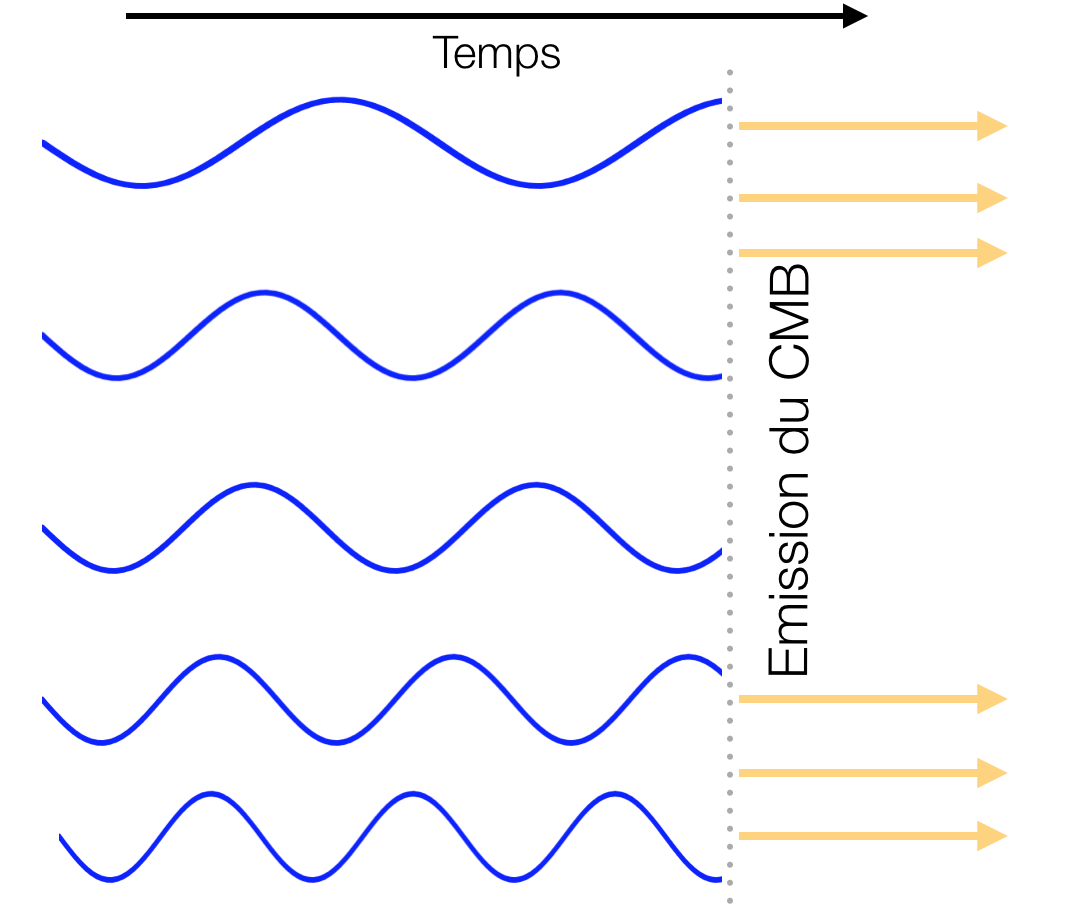
\includegraphics[height=12cm]{figs/bao1.png}
	\caption[Les oscillations baryoniques évoluent sur des fréquences différentes, dépendant de leur taille.]{Les oscillations baryoniques évoluent sur des fréquences différentes, dépendant de leur taille. Les grandes structures oscillent lentement, les petites rapidement. Certains modes vont être en extremum d'amplitude au moment de la recombinaison et donc au moment de la dernière diffusion du fond diffus cosmologique. Ces modes vont donc être privilégiés dans la carte du CMB.}
	\label{f:bao1}
\end{figure}


\newthought{Ces oscillations baryoniques}  sont des ondes accoustiques (BAOs, de l'anglais \textit{baryonic accoustic oscillations})\index{BAO} car elles sont entretenues par l'entrejeu entre gravité et pression (de rayonnement dans le cas présent). Par simple inspection de l'équation différentielle maîtresse, on peut constater que la fréquence d'oscillation dépend de la taille du mode étudié : un mode à grande fréquence spatiale implique une grande fréquence temporelle et vice-versa. Par conséquent, l'amplitude du mode au moment de la recombinaison va dépendre du mode en question : au moment de l'émission du fond diffus, certains modes seront en amplitude maximale, d'autres en amplitude plus modérée. En simplifiant, on peut imaginer que certains modes vont osciller un nombre de fois entier entre leur déclenchement et la recombinaison, parvenant ainsi à un extremum d'amplitude tandis que d'autres seront dans une phase quelconque avec des amplitudes moins remarquables. Les échelles qui se détachent sous la forme de 'pics' dans le spectre de puissance du fond diffus cosmologique sont la manifestation de ces modes qui parviennent en extremum d'amplitude au moment où le rayonnement fossile est produit.



\begin{figure}[htbp]
	\centering
		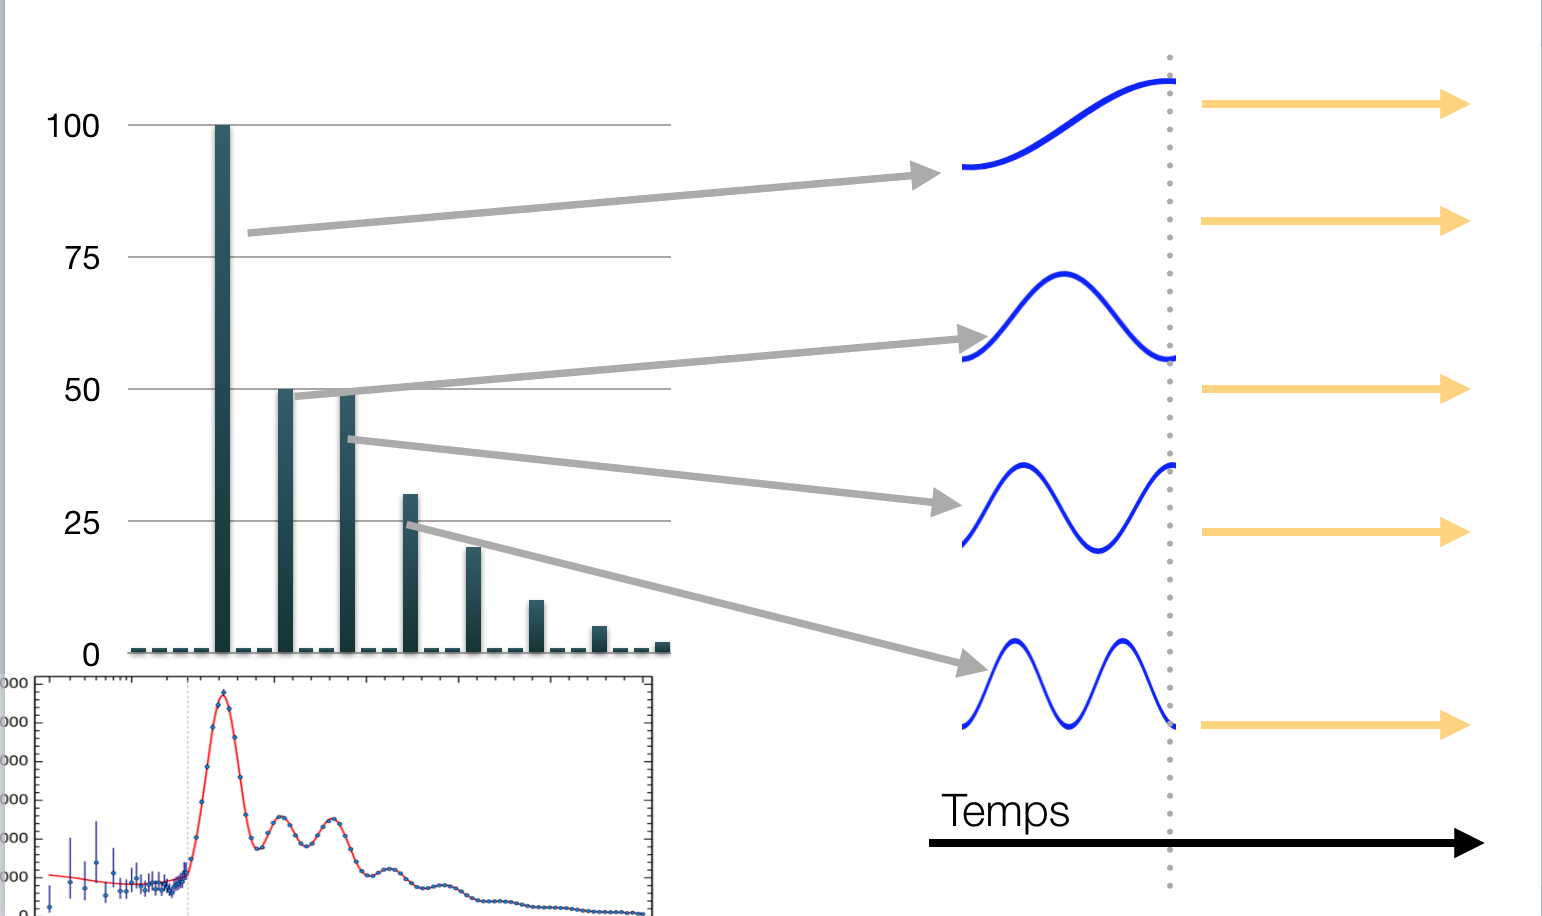
\includegraphics[height=12cm]{figs/bao2.png}
	\caption[Les pics accoustiques sont des extrema]{Les pics accoustiques du spectre de puissance du fond diffus cosmologique correspondent aux modes qui sont en extremum d'amplitude au moment de la recombinaison. Le premier pic correspond à une compression, le second une compression + une détente, le troisième une compression + une détente + une compression, etc.... Au premier ordre, nous voyons des harmoniques d'un même mode fondamental. }
	\label{f:bao2}
\end{figure}

\section{Croissance des perturbations : cas super-horizon}
\newthought{L'horizon}\index{horizon} désigne la plus grande échelle sur laquelle un phénomène de propagation peut opérer. Sa valeur est simplement donnée par :
\begin{equation}
L_H=\frac{c}{H}
\end{equation}
où $H^{-1}$ opère comme une mesure de l'âge de l'Univers à un instant donné. L'horizon est donc le produit de la plus grande vitesse par la plus grande durée. Son expression comobile présente une évolution temporelle qui dépend de la période de domination. Durant la période dominée par le rayonnement on a comme horizon comobile:
\begin{equation}
\ell_{H,RD}=\frac{c}{aH}\sim a
\end{equation} 
et durant la période dominée par la matière:
\begin{equation}
\ell_{H,MD}\sim\sqrt{a}.
\end{equation}
Dans les 2 cas, l'horizon grandit avec le temps et un mode de taille comobile donnée va donc successivement être plus grand que l'horizon (super-horizon) puis plus petit (sub-horizon). Le cas super-horizon demande un traitement en relativité générale complet donnant l'équation de croissance des structures suivantes:
\begin{equation}
\ddot \delta_k + 2H \dot \delta_k = \frac{3}{2}H^2(1+w)(1+3w)\delta_k
\end{equation}
où $w=0$ durant l'époque MD et $w=1/3$ durant l'époque RD \sidenote{pour ces échelles plus grandes que l'horizon, la pression ne peut jouer un role significatif: baryons et matière noire ont le même comportement}. 

Cette équation est similaire à celle obtenue dans le cas sub-horizon. Pour l'époque de domination de la matière on retrouve le même taux de croissance que celui obtenu pour la matière noire :
\begin{equation}
\delta_{k,MD}\sim t^{2/3}\sim a(t),
\end{equation}
tandis que durant l'époque de domination du rayonnement on obtient:
\begin{equation}
\delta_{k,RD}\sim t \sim a(t)^2.
\end{equation}


\section{Croissance des perturbations : synthèse et spectre de puissance}

La synthèse des résultats précédents pour le cas de la matière noire est présenté dans la figure \ref{f:perturb}. On constate qu'une petite perturbation peut voir son histoire de croissance gelée si elle passe sous l'horizon durant l'époque dominée par le rayonnement. A l'inverse un mode de grande longueur d'onde devra attendre la période dominée par la matière pour changer de régime et ne connaîtra pas la phase de non-croissance qu'aura connu les plus petites structures.

\begin{figure}[htbp]
	\centering
		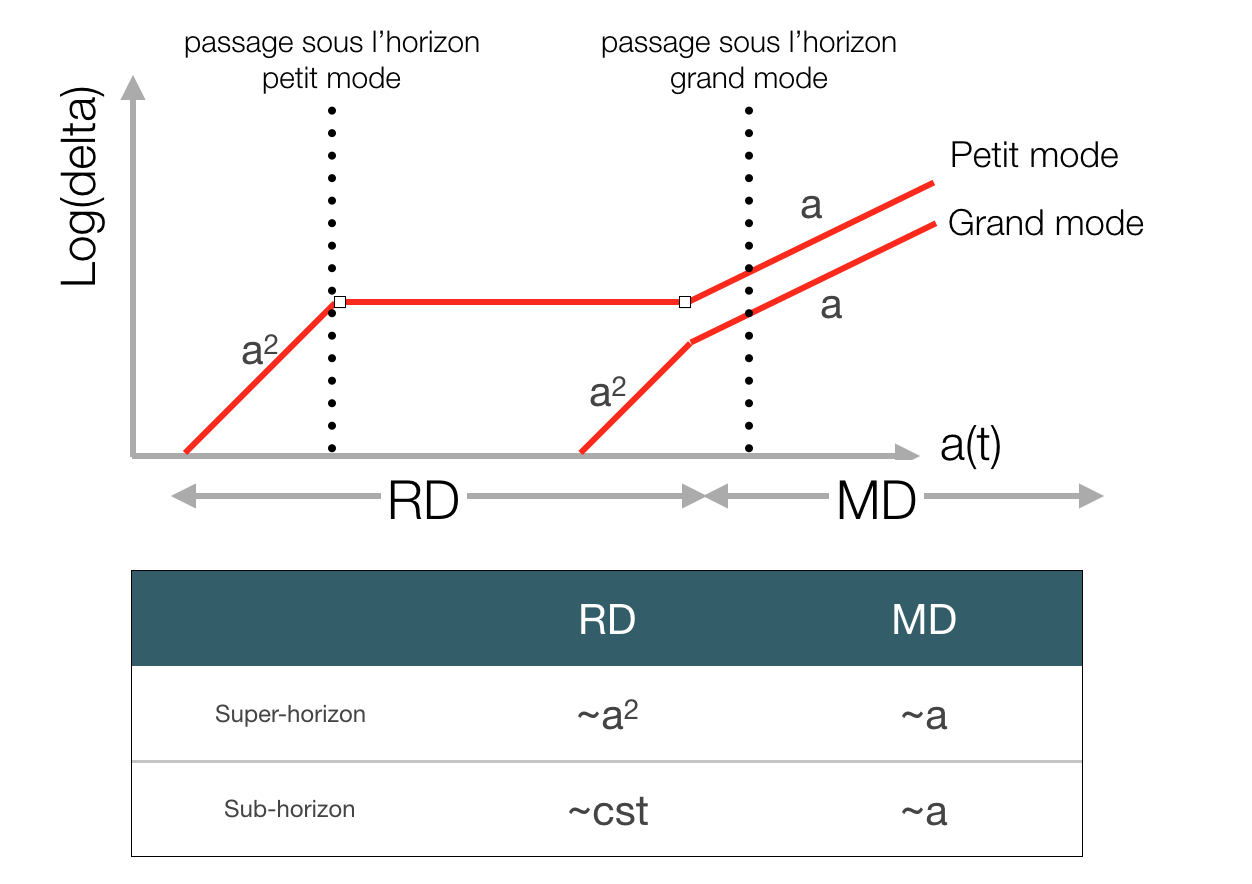
\includegraphics[height=8cm]{figs/perturb.png}
		\caption[Synthèse de la croissance des perturbations]{Synthèse de la croissance des perturbations. Un petit mode possède une taille caractéristique suffisemment petite pour passer sous l'horizon durant l'époque dominée par le rayonnement.}
	\label{f:perturb}
\end{figure}

Grâce à cette synthèse on peut prédire l'amplitude d'un mode au moment de la recombinaison $\delta_f$ en fonction de son amplitude $\delta_i$ bien avant l'équivalence matière-rayonnement. Considérons d'abord le cas d'un grand mode, sans période de gel de croissance, son amplitude au moment de l'équivalence est donné par:
\begin{equation}
\delta_e=\frac{a_e^2}{a_i^2}\delta_i.
\end{equation}
Son amplitude finale est alors donnée par :
\begin{equation}
\delta_f=\frac{a_f}{a_e}\delta_e=\frac{a_f a_e}{a_i^2}\delta_i.
\end{equation}
La chose importante est l'indépendance du facteur reliant l'amplitude initiale et finale vis à vis de la taille du mode : tous les modes vont croître dans les même proportions entre les instants $i$ et $f$. 

Pour les petits modes la situation est différente. L'amplitude au passage sous l'horizon est donnée par
\begin{equation}
\delta_L=\frac{a_L^2}{a_i^2}\delta_i.
\end{equation}
où $a_L$ est l'instant de passage sous l'horizon. L'amplitude au moment de l'équivalence est identique car la croissance est gelée et l'amplitude finale est alors donnée par:
\begin{equation}
\delta_f=\frac{a_f}{a_e}\delta_e=\frac{a_f}{a_e}\delta_L=\frac{a_L^2 a_f}{a_i^2 a_e}\delta_i.
\end{equation}
Ici le facteur de lien dépend de $a_L$ et donc de la taille du mode considéré. En effet cet instant est déterminé par $\lambda = \ell_{H,RD} \sim a_L$ donc 
\begin{equation}
\delta_f \sim \frac{1}{k^2} \delta_i.
\end{equation}
On a une coupure d'autant plus forte que la fréquence du mode est élevée, d'autant plus forte que la taille du mode considéré est petite.

\newthought{Pour le spectre de puissance}\index{spectre de Puissance}, les conséquences sont simples. Pour les $k$ suffisamment faibles on a 
\begin{equation}
P_f(k)\sim\delta_k^2 \sim P_i(k),
\end{equation}
par contre pour les hautes fréquences le spectre de puissance est filtré suivant la relation:
\begin{equation}
P_f(k)\sim \frac{1}{k^4} P_i(k)
\end{equation}
Comme le spectre de puissance primordial est en loi de puissance tel que \sidenote{on parle de spectre invariant d'échelle, comme prédit par exemple par l'inflation}:
\begin{equation}
P_i(k)\sim k
\end{equation}
on obtient un spectre caractéristique aux hautes fréquences en 
\begin{equation}
P_f(k)\sim\frac{1}{k^3}.
\end{equation}
Le spectre de puissance résultant possède donc 2 régimes caractéristiques, l'un aux grandes échelles en $P(k)\sim k$ et l'autre aux petites échelles en $P(k)\sim k^{-3}$. La transition entre les deux correspond à l'échelle qui passe sous l'horizon exactement au moment de l'équivalence (cf. Fig \ref{f:pk}).

\begin{figure}[htbp]
	\centering
		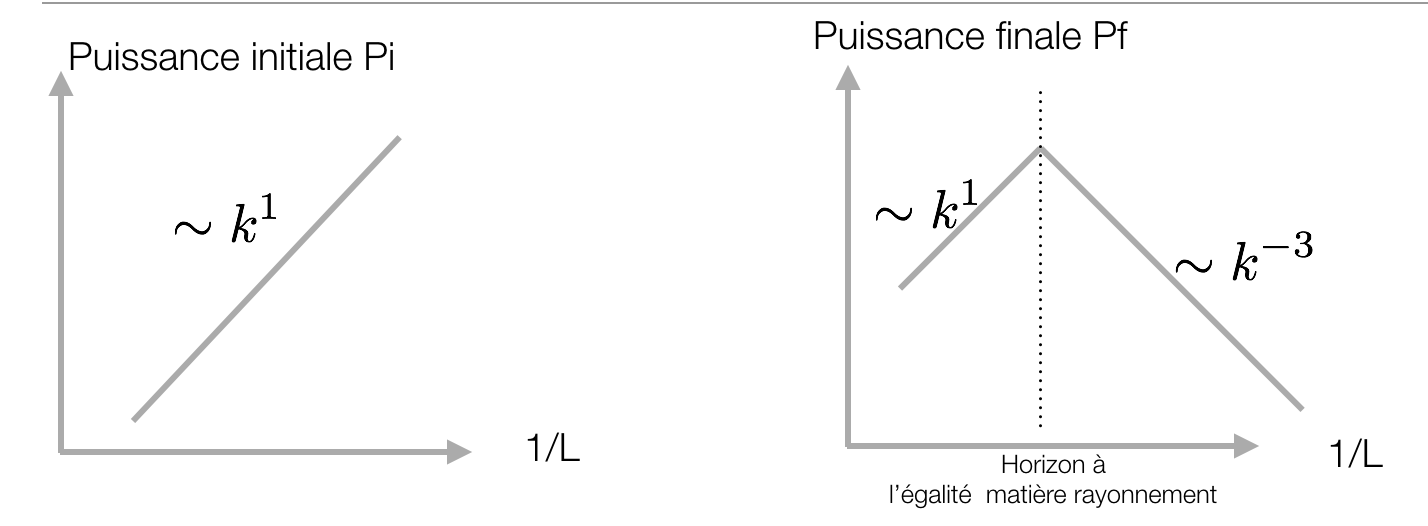
\includegraphics[height=8cm]{figs/pk.png}
		\caption[Schématique du filtrage du spectre de puissance des fluctuations initiales.]{Schématique du filtrage du spectre de puissance des fluctuations initiales. Le spectre primordial est invariant d'échelle en $P(k)\sim k$ et le gel de la croissance des fluctuations sous l'horizon durant l'époque de domination du rayonnement produit un filtrage au hautes fréquences qui produit une pente caractéristique en $P(k)\sim k^{-3}$.}
	\label{f:pk}
\end{figure}

\newthought{Pour résumer}, le spectre de puissance de la matière est une version filtrée du spectre de puissance primordial. Ce filtre opère sur les échelles suffisamment petites pour passer dans l'Horizon cosmologique tôt dans l'histoire de l'Univers, durant l'époque dominée par le rayonnement. Les échelles plus grandes ne permettant pas ce passage fréquence ont crû de façon indifférenciée et ont donc conservé les caractéristiques du spectre primordial. L'ensemble des prédictions développées dans ce chapitre, et notamment la mise en place du spectre de puissance $P(k)$ est fermement confirmée par de multiples observations (voir Fig. \ref{f:pktegmark})~: c'est un des grands succès du modèle $\Lambda$CDM aux grandes échelles.

\begin{figure}[htbp]
	\centering
		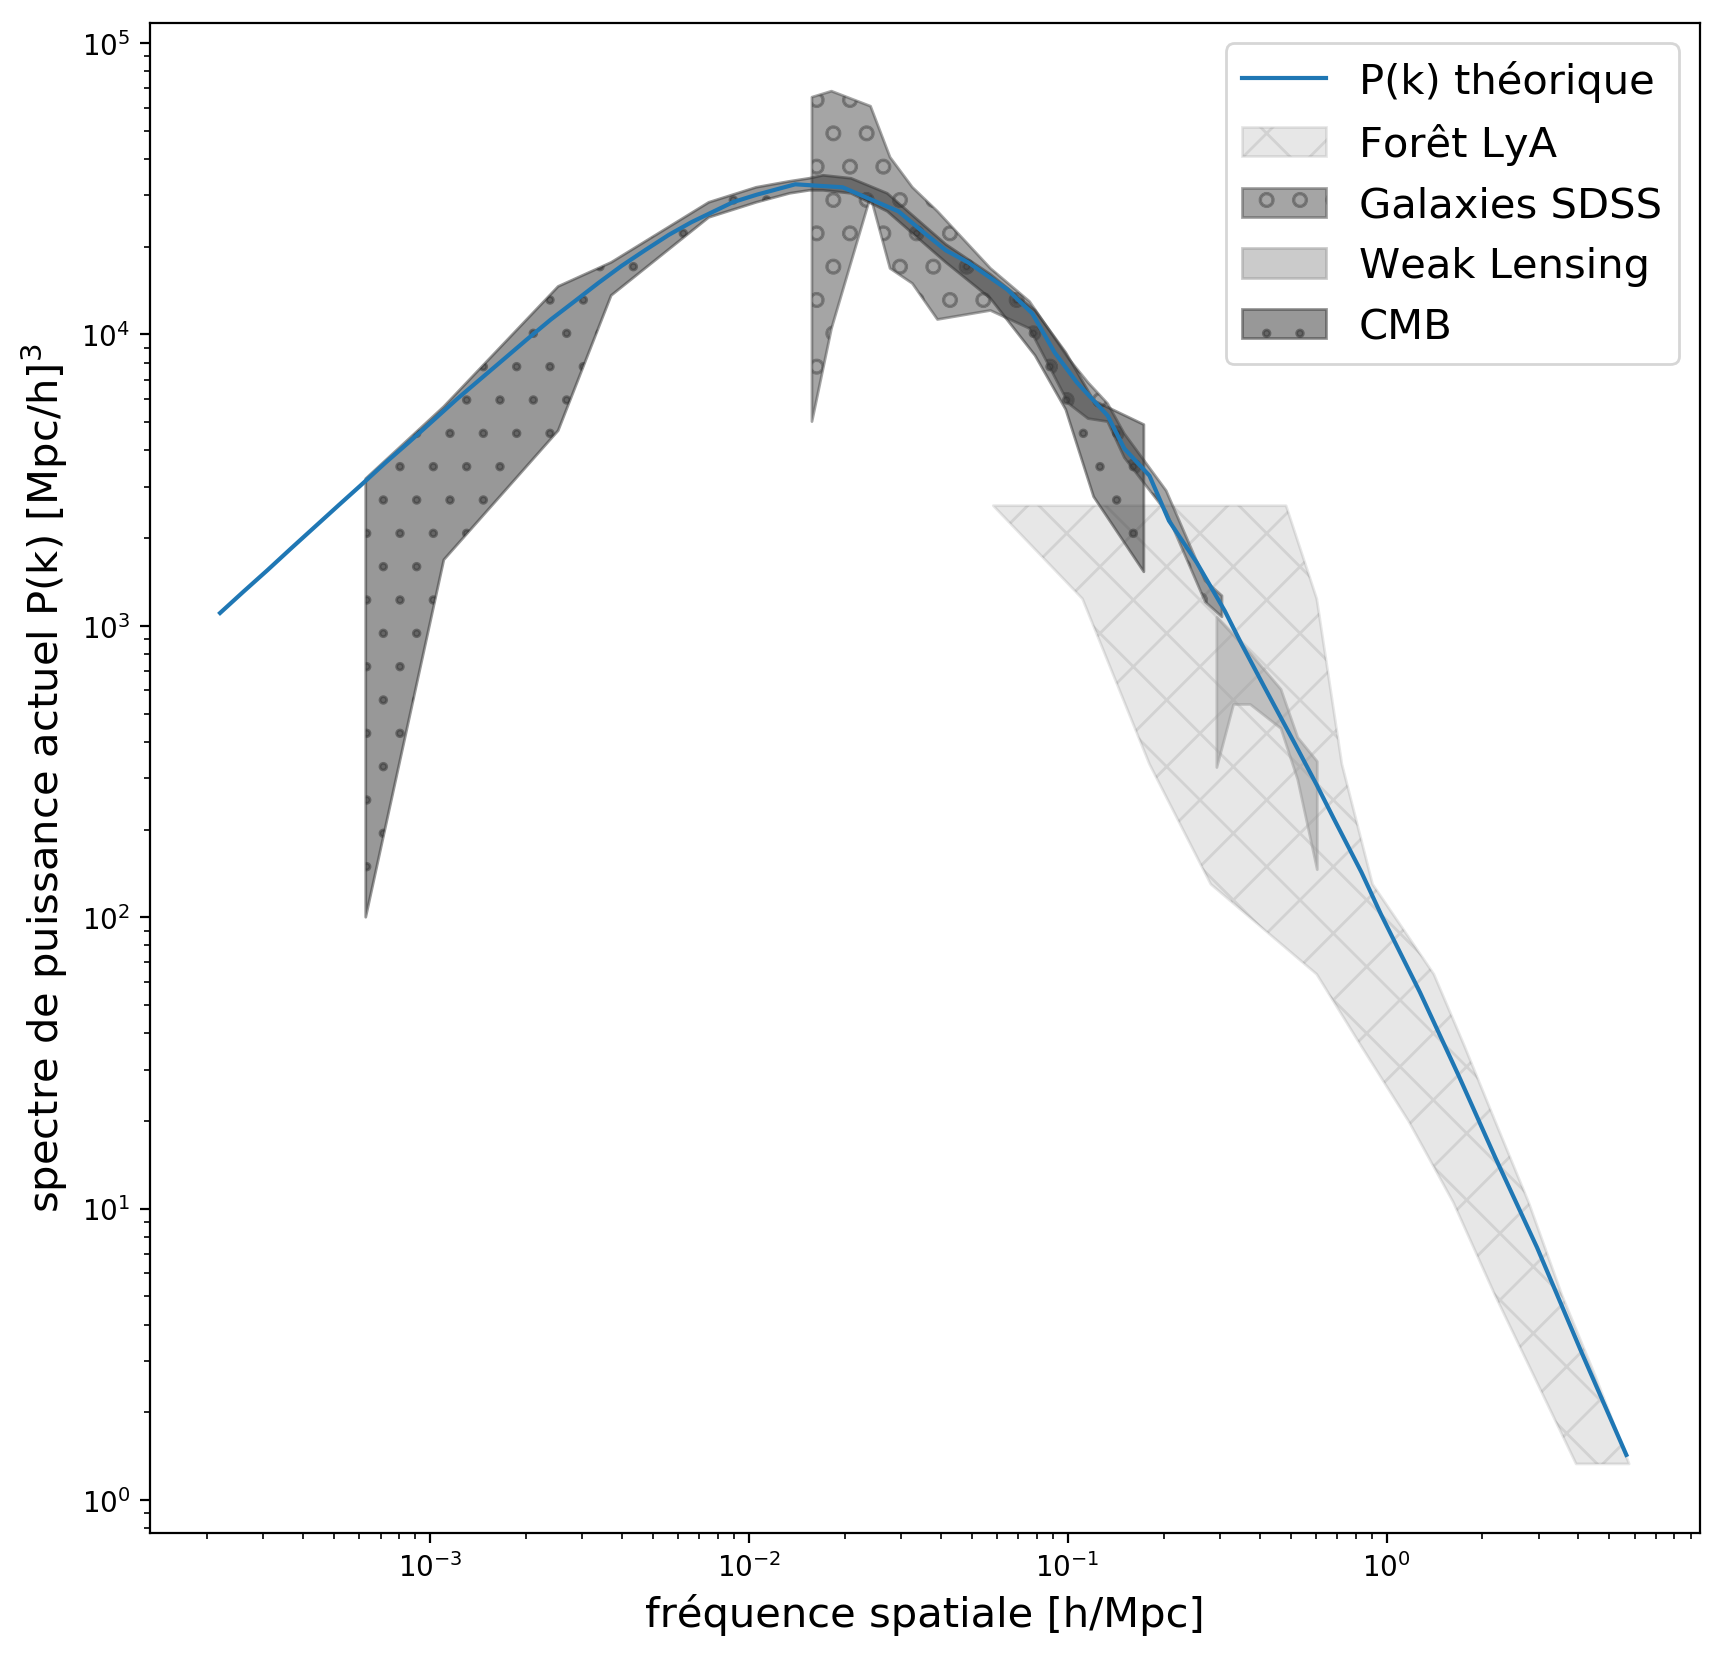
\includegraphics[height=12cm]{figs/pstegmark.png}
		\caption[Le spectre de puissance observé]{Le spectre de puissance $P(k)$ $\Lambda CDM$ théorique est représenté ici avec une compilation des estimations observationnelles issues de différentes sondes~: lensing, relevés de galaxies, CMB, comptage d'amas, Forêt Lyman-$\alpha$. On note l'excellent accord en théorie et prédiction.  Figure extraite de Tegmark et al. 2003. }
	\label{f:pktegmark}
\end{figure}


\newthought{Les oscillations baryoniques}\index{BAO}, mentionnées dans le cas de la matière avec pression et vues dans le CMB, se manifestent également dans le spectre de puissance de la matière totale. Ces ondes sonores se propageant dans le gaz vont légèrement modifier la structure globale de la matière : même si les baryons ne représentent qu'une faible fraction\sidenote{$\frac{\Omega_b}{\Omega_m}\sim0.15$} de la masse totale, cette fraction est non nulle et joue sur la dynamique globale à l'oeuvre. Ces oscillations se manifestent à nouveau comme des modes légèrement privilégiés dans le spectre de puissance $P(k)$. Par ailleurs, ces modes privilégiés vont persister dans la distribution de matière bien au delà de la recombinaison, jusqu'à nos jours. Par exemple, le spectre de puissance de la distribution actuelle des galaxies\sidenote{mesurée à z=0 dans des grands relevés de millions de galaxies comme le Sloane Digital Sky Survey (SDSS)}  présente des modes privilégiés aux fréquences attendues (voir Fig. \ref{f:percival}). De même, la distribution du gaz diffus intergalactique\index{IGM} à z=2\sidenote{sondée dans les spectres de Quasars distant} manifeste ces mêmes modes privilégiés. Ces ondes de pressions primordiales, on laissé leur empreinte dans toutes les structures qui ont émergé tout au long de l'histoire de l'Univers.

\begin{figure}[htbp]
	\centering
		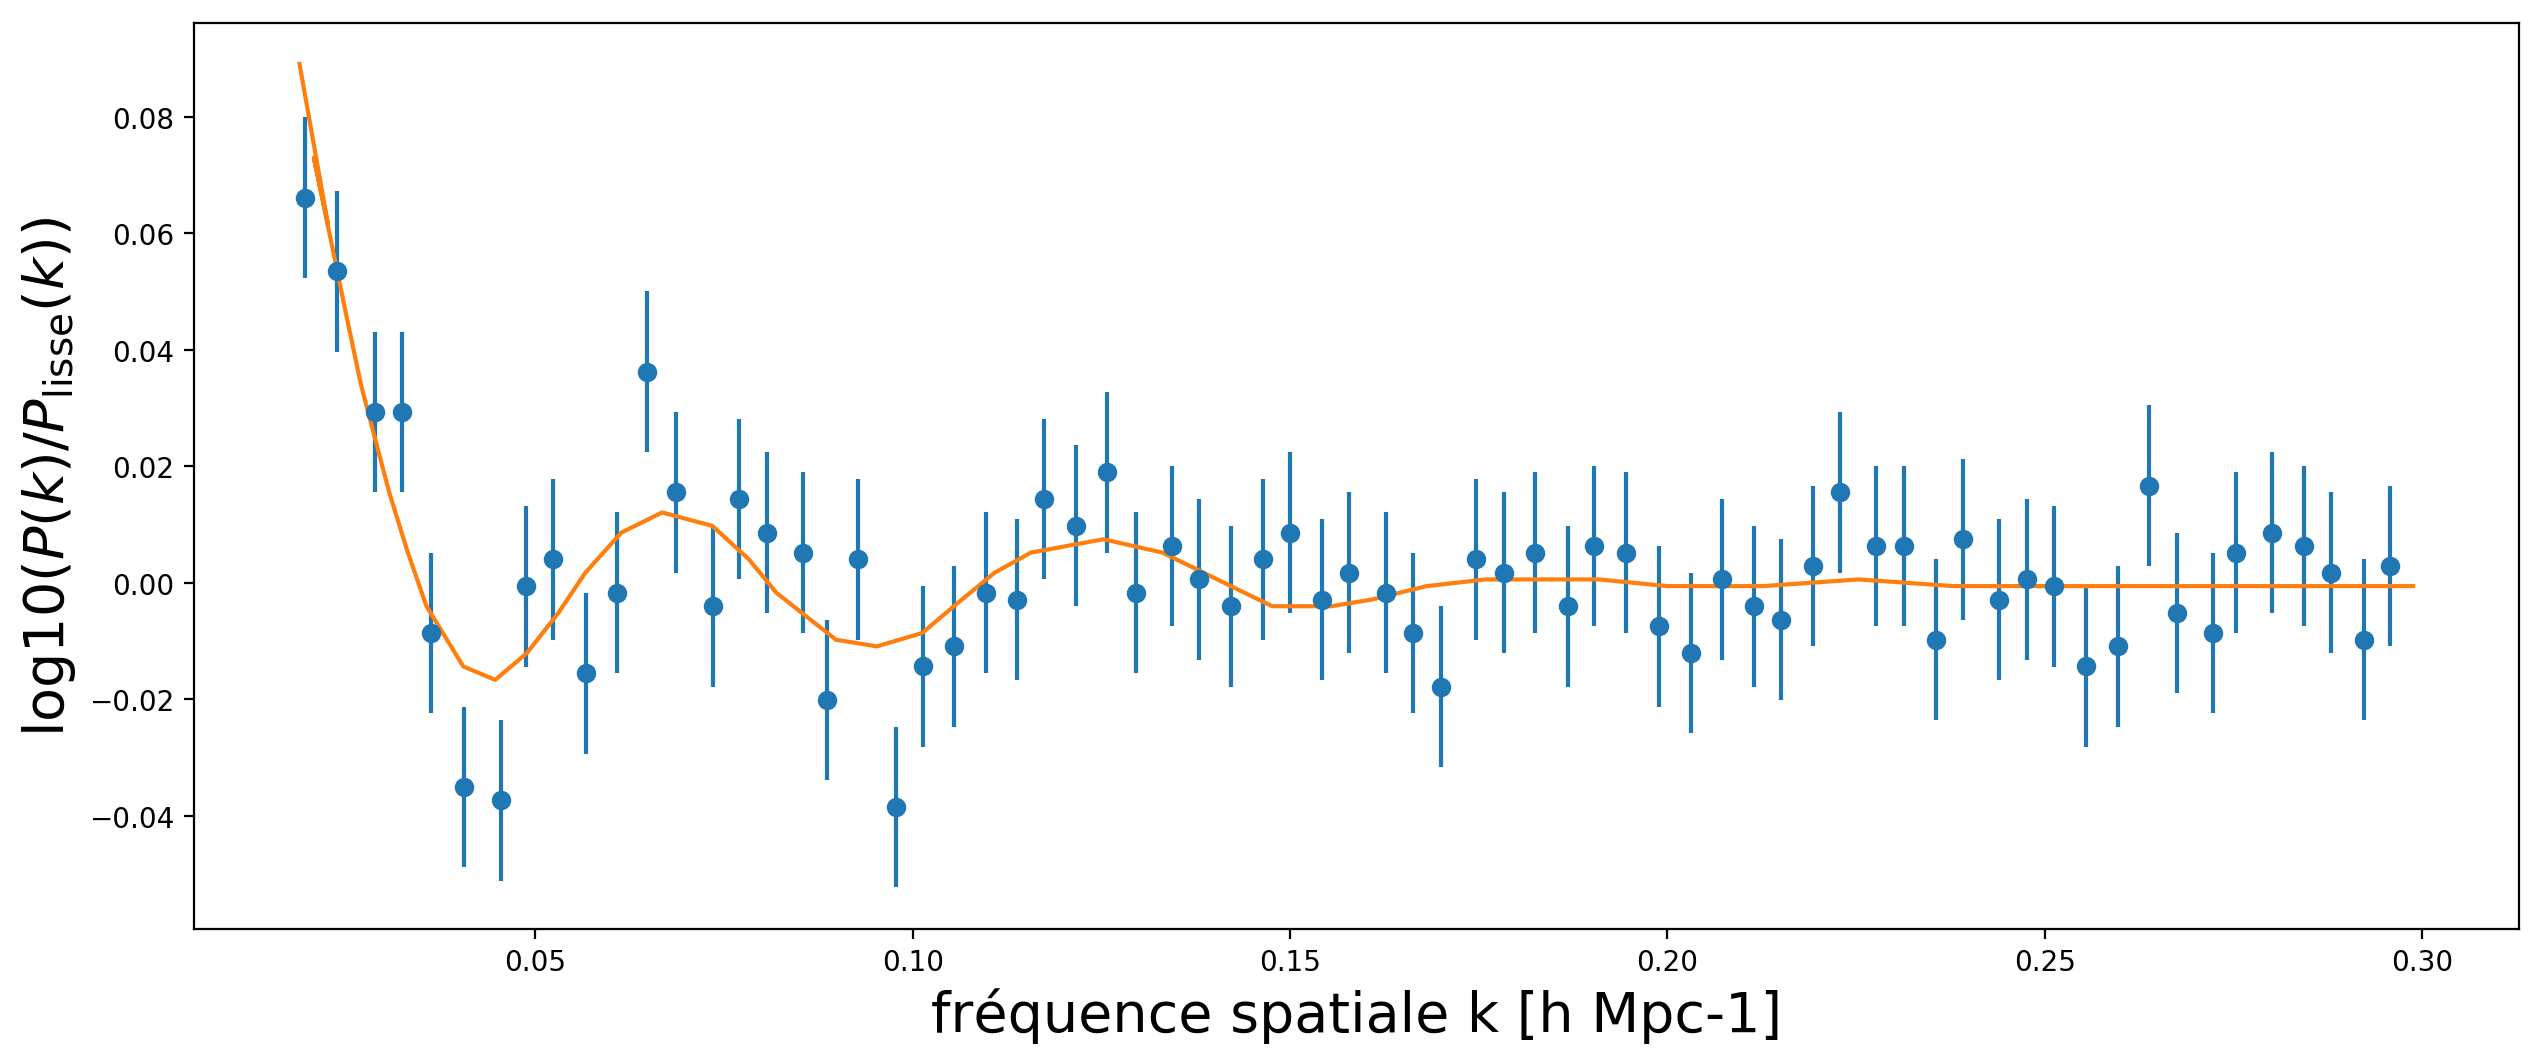
\includegraphics[height=12cm]{figs/percival.png}
		\caption[Les BAOs dans les relevés de galaxies]{Détection des BAOs dans le spectre de puissance du grand relevé de galaxies SDSS. Les courbes représentées sont le rapport du spectre mesuré dans les données sur le spectre lissé, sans BAO, pour 3 échantillons de galaxies différents. Les BAOs sont très clairement apparent (points) aux positions prédites par la théorie (lignes). Figure extraite de Percival et al. 2007.}
	\label{f:percival}
\end{figure}
\section{Et après ?}

Une fois le mécanisme d'instabilité déclenché, tous les modes vont parvenir à des régimes de surdensité qui vont au delà du régime linéaire et qui sortent du cadre dans lequel nous nous sommes placés. Dans certains cas académiques, le régime non linéaire peut-être abordé analytiquement mais en toute généralité il requiert l'utilisation de simulations numériques. La culmination de ce régime non linéaire est la création de structure denses, dominées par les baryons et au sein duquel se forment les sources de rayonnement : ce sont les galaxies qui nous entourent. L'apparition de ces objets est donc conditionnée par un contexte cosmologique et par extension il n'est pas illogique d'affirmer que l'étude de la formation des galaxies est une extension naturelle de la cosmologie. Toutefois, des phénomènes astrophysiques commencent à rentrer en jeu aux échelles considérées : thermodynamique du gaz, processus physico-chimique de refroidissement, champ magnétique, formation et rétroaction stellaire, production et impact des éléments plus lourds que l'hélium, etc.... Chacun de ces phénomènes est un objet d'étude à part entière et chacun de ces phénomènes est compris de façon toute relative. On en décrira quelques uns dans un chapitre dédié, mais de façon générale on peut aisément avancer qu'aujourd'hui l'extension de la théorie cosmologique à celle de la formation des galaxies présente des défis majeurs. Ces défis, à l'heure où ces lignes sont écrites ne sont pas résolus.

%\chapter{Formation des 'petites' structures}
\newthought{Une surdensité de matière} va nécessairement sortir du régime des faibles valeurs au bout d'un certain temps : le mécanisme d'instabilité gravitationnelle va condenser les structures vers des grandes densités et le jeu d'équations linéarisées utilisé dans le chapitre précédent n'est plus valable. Nous allons ici développer un modèle simple de surdensité qui permet de suivre l'évolution d'une telle structure en effondrement \index{effondrement sphérique}. Le destin d'une telle structure est de finir en halo de matière\index{halo}\sidenote{et donc dominé par la matière noire} à l'équilibre, dont on exposera aussi les propriétés de base. A des fins de simplification, nous allons par la suite nous limiter au cas d'un Univers rempli uniquement de matière noire, non-collisionnelle, avec $\Omega_m=1$. Comme vu précédemment, cet Univers de Einstein-de Sitter\index{Einstein- de Sitter} est régi par une expansion en :
\begin{equation}
a(t) \sim t^{2/3}.
\end{equation}

\section{Au-delà du régime linéaire : le modèle d'effondrement sphérique\index{effondrement sphérique}}

Considérons une surdensité, sphérique de rayon $r$, baignant dans un Univers de densité $\bar \rho$. A l'intérieur de cette surdensité, la densité est initialement légèrement plus grande que celle du fond avec $\rho = (1+\delta) \bar \rho$ et uniforme à l'intérieur de ce rayon \sidenote{On parle aussi de modèle 'chapeau haut-de-forme' \index{haut-de-forme} à cause du profil de densité en créneau associé }.  Ce modèle ressemble grandement au modèle de cosmologie newtonienne \index{cosmologie newtonienne} abordé en début d'ouvrage : dans ce modèle de cosmologie et pour la surdensité qui nous intéresse, sa dynamique est régie uniquement par la matière qui se trouve à l'intérieur et la couche la plus externe de la surdensité suit le principe fondamental de la dynamique\index{principe fondamental de la dynamique} :
\begin{equation}
\ddot r = -\frac{GM(<r)}{r^2}.
\end{equation}
Rappelons que $r(t)=a(t)r_0$ et dans le cas où cette couche est en expansion infinie \sidenote{ avec $\dot a >0$}, on peut facilement intégrer l'équation différentielle précédente pour obtenir :
\begin{eqnarray}
\dot a &=&\sqrt{\frac{2GM(<r)}{ar_0^3}}\\
r(t)&=&\left(\frac{9GM(<r)}{2}\right)^{1/3} t^{2/3}
\end{eqnarray}
avec une dépendance temporelle en $t^{2/3}$ conforme au modèle Einstein - de Sitter\index{Einstein-de Sitter}. Toutefois, cette dépendance ne peut représenter l'effondrement d'une structure, puisqu'on attend d'elle que son rayon diminue au delà d'un certain temps\sidenote{donc l'hypothèse $\dot a >0$ ne tient plus et nous empêche d'intégrer simplement l'équation différentielle}.

\newthought{Un bon point de départ} est l'équation de conservation de l'énergie spécifique de la couche externe de notre structure :
\begin{equation}
E=\frac{\dot r^2}{2}-\frac{GM}{r}
\end{equation}
où $M=M(<r)$ désigne la masse à l'intérieur de la couche la plus externe. Rappelons que dans ce type de modèle les couches ne se croisent pas \sidenote{comme indiqué par $r(t)=a(t)r_0$ : une couche externe reste toujours une couche externe} et cette masse interne $M$ reste constante. Enfin, notre structure est vouée à s'effondrer, son énergie mécanique\index{energie!mécanique} totale est donc négative, $E<0$. Dans ce type de situation, on peut montrer que la solution $r(t)$ s'exprime sous forme \textit{paramétrique} (voir aussi la figure \ref{f:rtparam}):
\begin{eqnarray}
r(\theta)&=&A (1-\cos \theta)\\
t(\theta)&=&B (\theta-\sin \theta)
\end{eqnarray}
où $\theta$ est un paramètre tel que $\theta \in [0,2\pi]$. La vitesse de la couche peut également s'écrire sous forme paramétrique\sidenote{obtenue en dérivant l'équation sur le temps puis en l'injectant dans celle sur le rayon}:
\begin{equation}
v(\theta)=\dot r= \frac{A \sin \theta}{B(1-\cos \theta)}.
\end{equation}
Ici, $A$ et $B$ sont respectivement des rayons et temps caractéristiques du problème traité avec :
\begin{eqnarray}
A&=&\frac{GM}{2|E|}\\
B&=&\frac{GM}{(2|E|)^{3/2}}\\
A^3&=&GM B^2
\end{eqnarray}
où la dernière relation est similaire à la troisième loi de Kepler qui relie période et rayon des orbites autour d'un corps massif.


\begin{figure}[htbp]
	\centering
		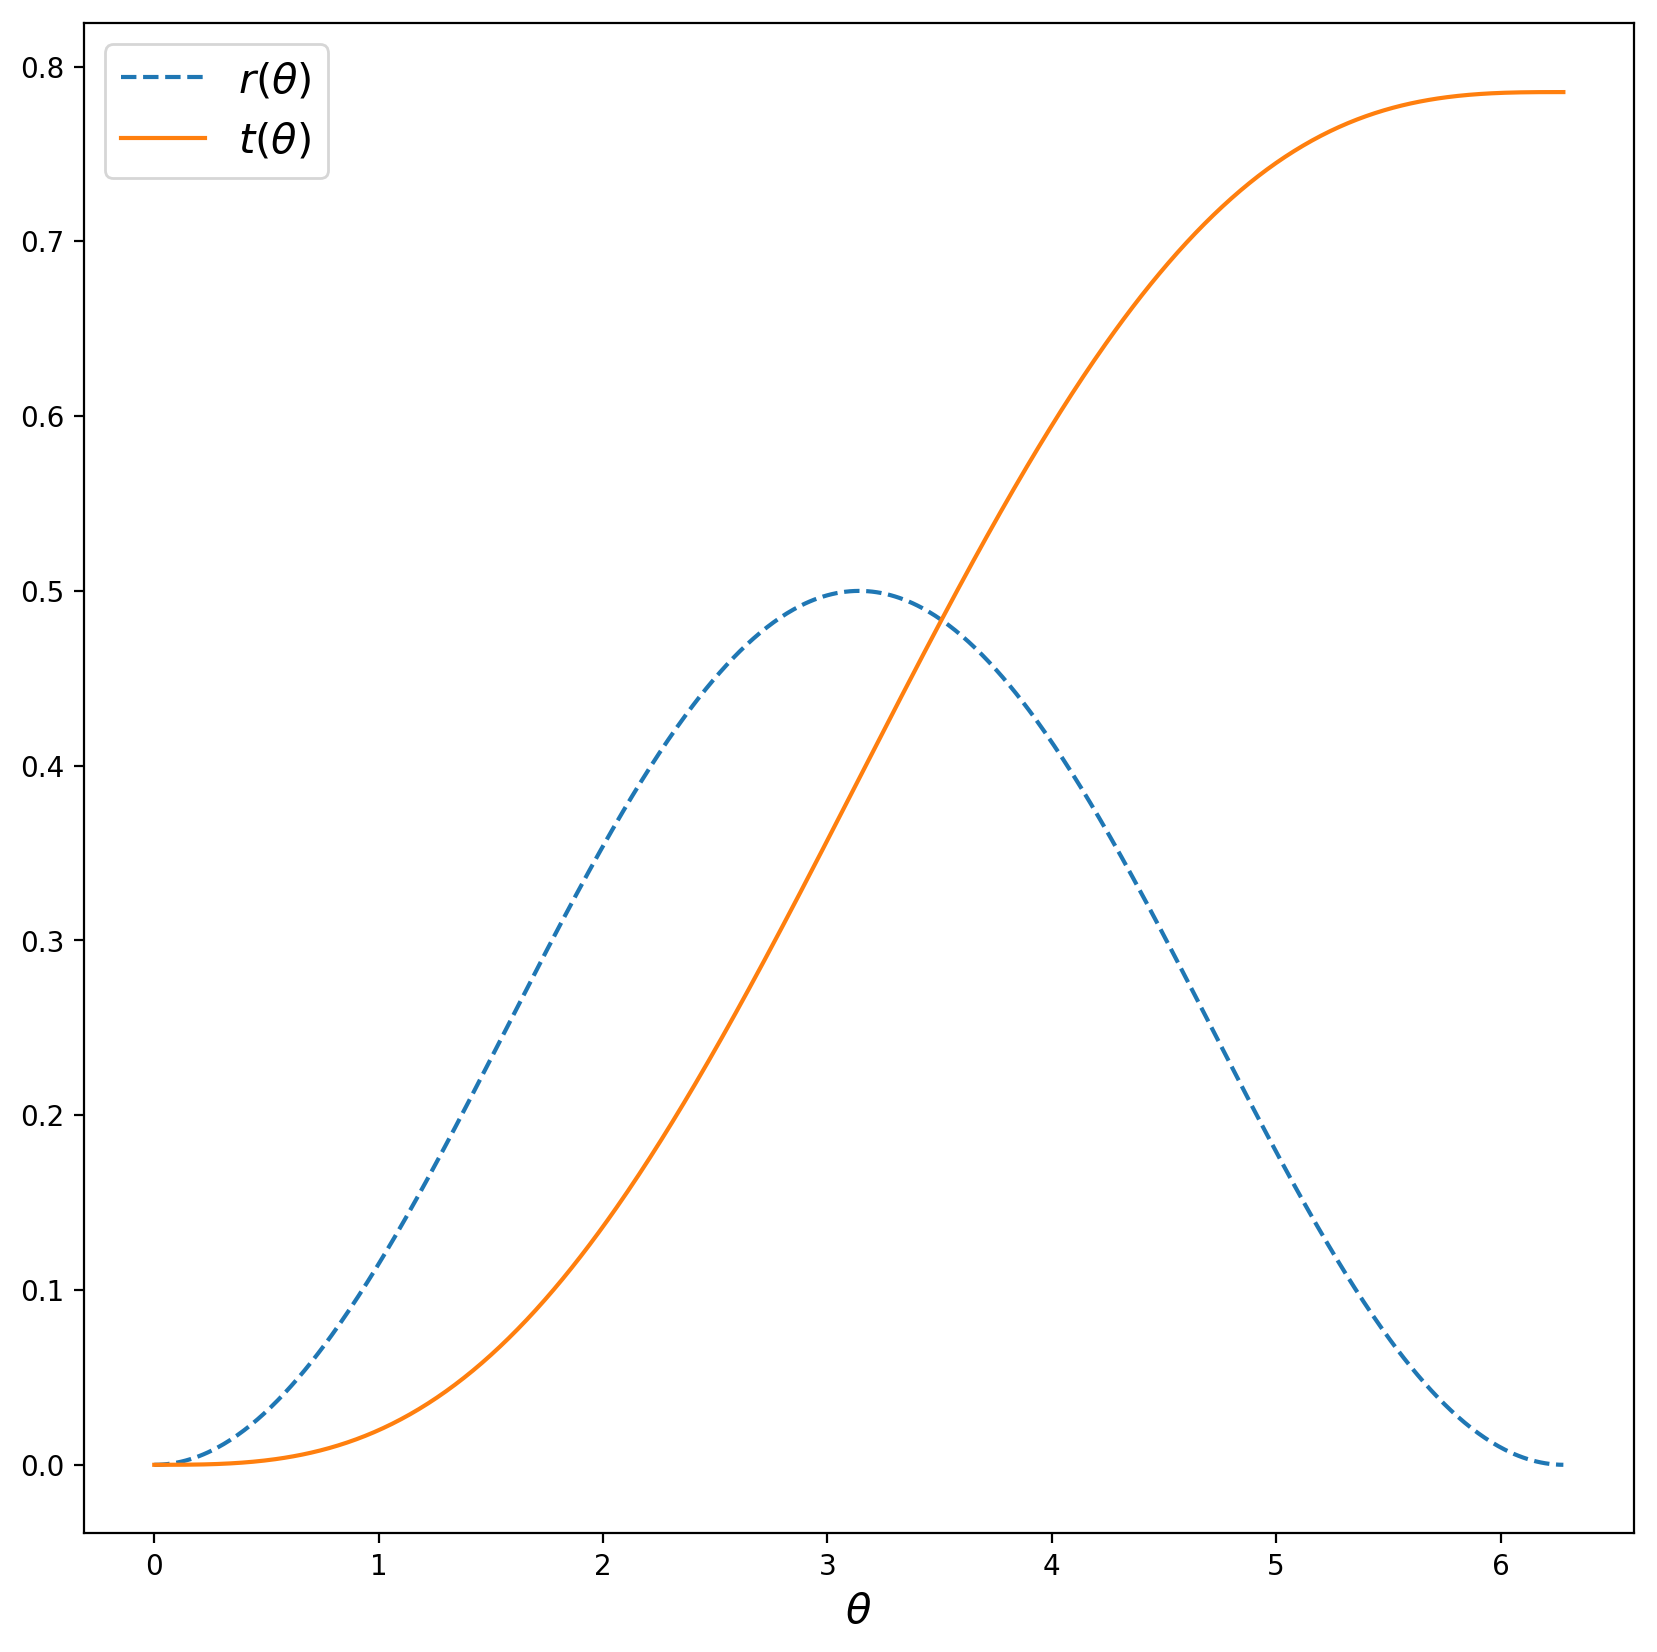
\includegraphics[height=10cm]{figs/rtparam.png}
		\caption[Les solutions paramétriques de l'effondrement sphérique]{Les solutions du modèle d'effondrement sphérique en fonction du paramètre $\theta$. Le temps $t$ est une fonction monotone de ce paramètre tandis que le rayon de la surdensité passe par un maximum, correspondant au découplage de la structure par rapport au fond cosmologique, avant de tendre vers 0 à la fin de l'effondrement.}
	\label{f:rtparam}
\end{figure}

Ces relations paramétriques permettent de caractériser les grandes étapes du processus d'effondrement. D'abord, on constate que l'évolution du rayon n'est pas monotone, celui-ci croît, atteint un maximum et décroit pour devenir nul : notre surdensité évolue d'abord avec le fond, suivant l'expansion globale, puis elle atteint une extension maximale avant de se \textit{découpler} du flot global. La structure se réduit en taille avant d'atteindre une extension nulle et par conséquent sa densité devient infinie ! Cette évolution \sidenote{qui est la même que celle d'un Univers de densité supérieure à la densité critique} conduit naturellement à des régimes de densité non linéaires\index{régime non-linéaire}. Par simple inspection, on constate que le découplage\index{expansion!découplage}, correspondant au maximum de $r$, opère pour $\theta=\pi$ et 
\begin{eqnarray}
r_d&=&2A\\
t_d&=&\pi B.
\end{eqnarray}
L'effondrement final correspond quant à lui à $\theta=2 \pi$ et 
\begin{eqnarray}
r_e&=&0\\
t_e&=&2\pi B.
\end{eqnarray}
Le temps nécessaire à l'effondrement\index{effondrement sphérique} \sidenote{on utilise aussi fréquemment les termes anglais de \textit{turn-around} pour le découplage et de \textit{collapse} pour l'effondrement} total de la structure est le double de celui nécessaire au découplage : $t_e=2 t_d$.

\newthought{La surdensité varie aussi de façon paramétrique}. La densité à l'intérieur de la structure est donnée par :
\begin{equation}
\rho = \frac{M}{4/3 \pi r^3}=\frac{3M}{4\pi A^3(1-\cos \theta)^3}, 
\end{equation}
tandis que la densité du fond, égale à la densité critique dans notre modèle est donnée par \sidenote{on rappelle que $H=\frac{\dot a}{a}$ et $a\sim t^{2/3}$ dans Einstein- de Sitter}:
\begin{equation}
\bar \rho =\frac{3H^2}{8\pi G}=\frac{1}{6\pi G t^2}=\frac{1}{B^2 6\pi G (\theta-\sin \theta)^2}.
\end{equation}
On obtient alors la formulation paramétrique de l'évolution de la surdensité :
\begin{equation}
\frac{\rho}{\bar \rho}=1+\delta=\frac{9}{2}\frac{(\theta - \sin \theta)^2}{(1-\cos \theta)^3}.
\label{e:dcoll}
\end{equation}
Bien sûr, cette équation ne rend pas compte des phases ultimes de l'effondrement : cet effondrement doit s'arrêter lorsqu'un équilibre est atteint après réorganisation de la matière et des vitesses. Les coquilles se croisent\index{croisement de coquille}, la masse à l'intérieur de la coquille change et de l'énergie est échangée entre les couches.  

Toutefois, une bonne approximation du processus à l'oeuvre peut être obtenue en invoquant le théorème du viriel\index{théorème du viriel}. Une fois l'équilibre atteint, notre couche externe doit satisfaire
\begin{equation}
2 T +U = 0,
\end{equation}
où $T$ et $U$ désignent respectivement l'énergie cinétique\index{energie cinétique}\index{energie potentielle} et potentielle de notre couche externe après viriélisation. Comme par ailleurs l'énergie reste conservée, l'énergie totale en fin de viriélisation est donnée par:
\begin{equation}
E=\frac{U}{2}=-\frac{GM}{2r_v}
\end{equation}
où l'on considère que la masse interne n'a pas été modifiée significativement par la redistribution. A l'équilibre, la couche ne bouge plus et son énergie totale est complètement définie par son énergie potentielle : c'est également le cas lors du découplage, durant lequel l'énergie cinétique est nulle par définition et \sidenote{en effet le découplage correspond au maximum d'extension de la surdensité avec $\dot r=0$ par définition}
\begin{equation}
E=-\frac{GM}{r_d}.
\end{equation}
Par conservation de l'énergie de la couche et en combinant ces deux derniers résultats, on obtient une relation entre le rayon de la couche externe à l'équilibre $r_v$ et celui lors du découplage $r_d$:
\begin{equation}
r_v\sim \frac{1}{2}r_d,
\end{equation}
le rayon de la structure se stabilise autour d'une valeur correspondant à la moitié du rayon lors du découplage. Ce rayon est aussi appelé \textit{rayon de viriel}\index{rayon de viriel}, et est utilisé de façon générique pour désigner les bords 'externes' d'un halo de galaxie.

On peut également évaluer la valeur de la surdensité finale après la phase de viriélisation. On cherche à évaluer
\begin{equation}
1+\delta_\mathrm{v}=\frac{\rho(t_v)}{\bar \rho(t_v)},
\end{equation}
ce qui nécessite d'évaluer les deux densités $\rho$ et $\bar \rho$ post-viriélisation. La densité du fond est simple à obtenir, car la viriélisation opère au temps $t_v=t_e=2t_d=2\pi B$, on obtient donc:
\begin{equation}
\bar \rho(t_v) = \frac{1}{6\pi G t_v^2}=\frac{1}{4}\bar \rho (t_d).
\end{equation} 
De même, sachant que le rayon de viriel est la moitié du rayon de découplage, il existe une relation simple\sidenote{sachant que $r_v=r_d/2$} entre la densité à l'équilibre et celle lors du découplage:
\begin{equation}
\rho(t_v)=\frac{3 M}{4\pi r_v^3}=8 \rho(t_d)
\end{equation}
d'où la relation :
\begin{equation}
1+ \delta_v=\frac{8 \rho(t_d)}{\frac{1}{4}\bar \rho (t_d)}=32(1+\delta_d).
\end{equation}
Sachant que le découplage opère pour $\theta =\pi$, l'évaluation de l'équation \ref{e:dcoll} pour cette valeur donne $\delta_d\sim 5.55$ et une valeur de densité à l'équilibre 
\begin{equation}
1+\delta_v \sim 178.
\end{equation} 
En résumé, une structure qui s'effondre sous l'effet de l'instabilité gravitationnelle voit sa densité se stabiliser autour de 200 fois celle du fond. Pour cette raison, on désigne fréquemment le rayon de viriel $r_v$\index{rayon de viriel} sous le terme de $r_{200}$ et par exemple, c'est comme cela qu'on détermine l'extension d'un halo de galaxie dans une simulation numérique : son extension est choisie de telle façon à ce que la surdensité interne soit proche de 200.

\newthought{On peut également proposer une extrapolation linéaire\index{effondrement sphérique!extrapolation linéaire}} du calcul qui vient d'être réalisé. Il s'agit de calculer la surdensité au moment de l'effondrement mais telle qu'elle est prédite dans le régime linéaire. L'intérêt d'un tel calcul est qu'il permet de prédire simplement les régions qui vont s'effondrer sans avoir à réaliser un calcul non-linéaire complet : en se donnant un champ de densité, on peut prédire aisément sa croissance linéaire et désigner quelles régions vont s'effondrer et à quel instant. Si l'on reprend notre modèle paramétrique, le régime des faibles perturbations est celui qui opère au début, donc quand $\theta \ll 1$. Ce paramètre devient alors une simple fonction de $t$\sidenote{obtenu via un développement limité de $t(\theta)$} :
\begin{equation}
\theta \sim \left(\frac{6t}{B}\right)^{1/3}.
\end{equation}
De même dans ce régime et en utilisant les bons développements limités
\sidenote{on rappelle que $\cos \theta \sim 1-\theta^2/2+\theta^4/24$ et $\sin \theta \sim \theta -\theta^3/6 +\theta^5/120$.}
, l'équation \ref{e:dcoll} peut être réécrite :
\begin{equation}
1+\delta =\frac{9}{2}\frac{(\theta -\sin \theta)^2}{(1-\cos \theta)^3}\sim 1+\frac{3}{20} \theta^2.
\end{equation}
D'où l'expression de $\delta_l$ dans le régime linéaire en fonction du temps:
\begin{equation}
\delta_l=\frac{3}{20}\left(\frac{6t}{B}\right)^{2/3}=\frac{3}{20}(6\pi)^{2/3}\left(\frac{t}{t_d}\right)^{2/3}.
\end{equation}
On note d'ores et déjà que l'on retrouve la fameuse dépendance en $t^{2/3}$, propre aux modèles dominés par la matière. Au moment de l'effondrement, $t=t_e=t_v=2t_d$, ce qui donne $\delta_l=1.69$. Cette valeur revêt un caractère un peu 'magique' pour les cosmologues : si on évolue un champ de densité linéairement, les régions qui dépassent ce seuil vont s'effondrer. Ce type de raisonnement permet de prédire quelles régions vont former des structures et à quel instant : c'est ce qui permet par exemple de faire des prédictions analytiques sur la fonction de masse des halos de matière noire\sidenote{voir le chapitre dédié à la matière noire} ou bien sur leur histoire de formation. Ce types de prédictions sont à la base de modèles \textit{analytiques} de formation des galaxies où la connaissance de l'histoire de formation de ces objets obtenue par cette méthode peut être utilisée pour prédire l'évolution des baryons en leur sein et les propriétés des galaxies qui s'y forment.

\begin{figure}[htbp]
	\centering
		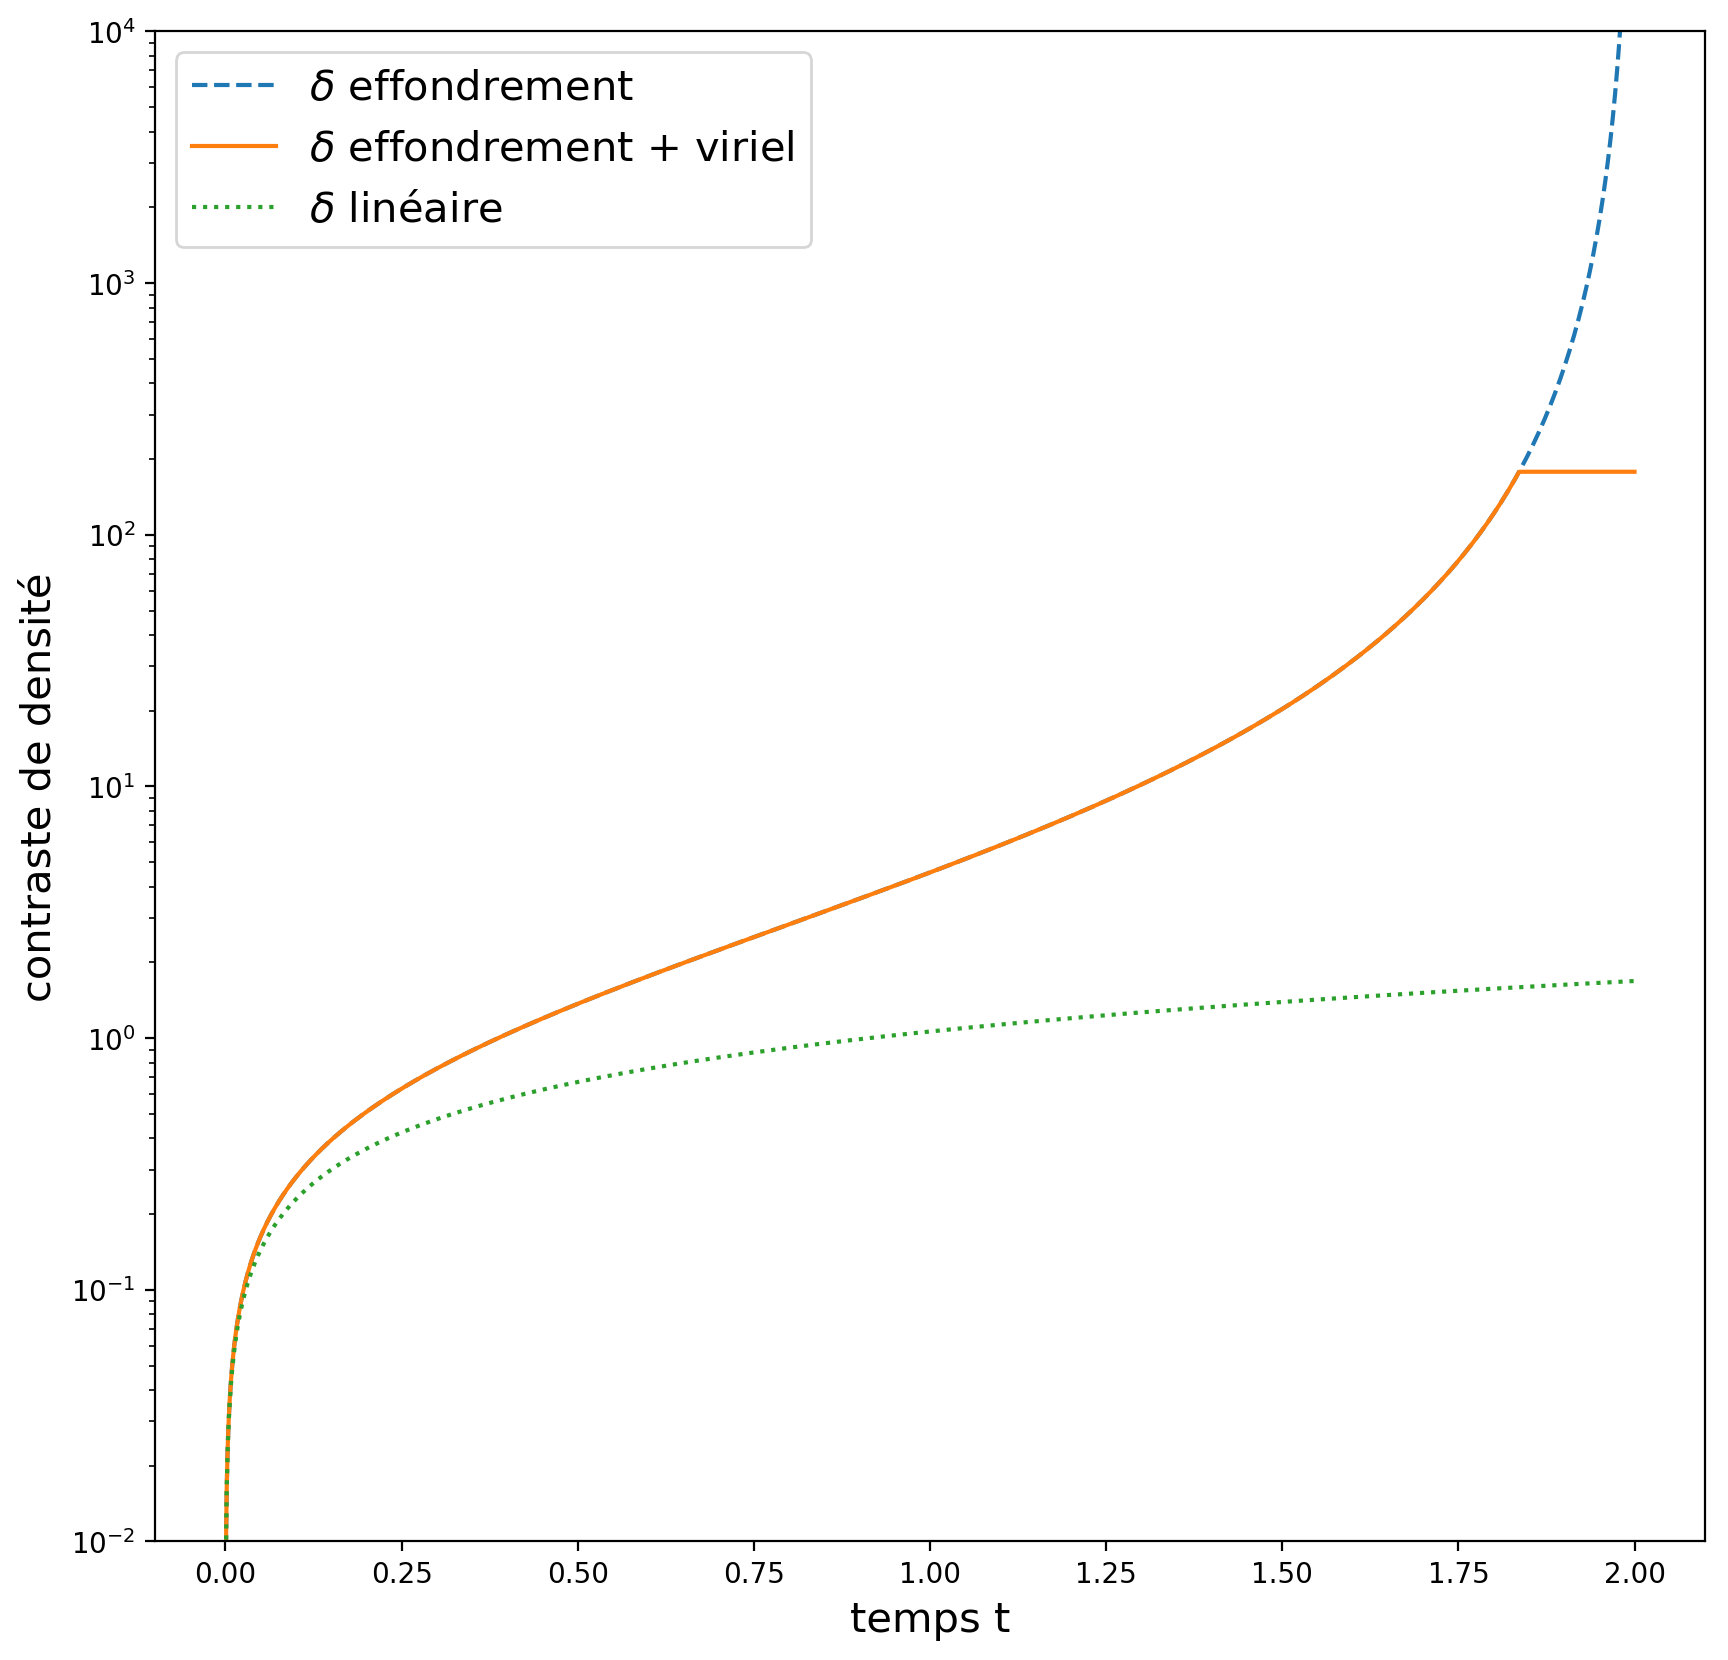
\includegraphics[height=10cm]{figs/delta_coll.png}
		\caption[Evolution temporelle du contraste de densité pour l'effondrement sphérique]{
		Les différentes solutions pour le contraste de densité $\delta=\rho/\bar \rho -1$ au cours du temps. On constate que le contraste non-linéaire évolue vers une singularité au moment de l'effondrement, la densité tend vers l'infini. Pratiquement, la surdensité va se stabiliser autour d'un contraste d'environ 200, correspondant à un état d'équilibre issu d'une redistribution de la matière et des vitesses appelée viriélisation. L'approximation linéaire
		 suit la solution non-linéaire dans le régime des petits contrastes mais évolue plus lentement aux temps ultérieurs pour atteindre une valeur de 1.68 au moment où la structure devrait s'effondrer.
		}
	\label{f:dcoll}
\end{figure}


\section{Propriétés générique des halos post-effondrement}
Les structures effondrées étudiées ici sont de fait les halos de matière noire\index{halo} qui entourent les galaxies. Nous venons par exemple de prédire que la densité typique interne à ces objets doit être de l'ordre de 200 fois celle du fond, mais qu'en est-il du profil de densité de ces halos ? Les simulations cosmologiques montrent que le profil résultant de la viriélisation est de forme \textit{ universelle} et qu'une forme fonctionnelle simple permet d'ajuster le profil de la distribution de matière sur des grandes gammes de masses d'objet. La plus célèbre de ces formes fonctionnelles est le profil NFW\index{profil NFW} \sidenote{du nom de ses découvreurs Navarro, Frenk et White} : 
\begin{equation}
\rho(r)=\frac{\rho_s}{(r/r_s)(1+r/r_s)^2}.
\end{equation}

\begin{figure}[htbp]
	\centering
		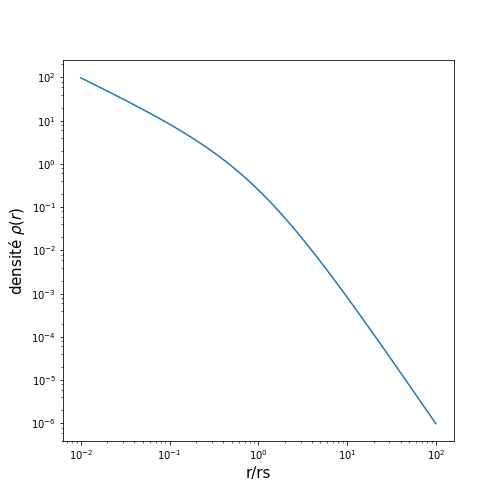
\includegraphics[height=9cm]{figs/nfw.png}
		\caption[Le profil de densité NFW]{Le profil de densité de NFW est le profil universel des halos de matière noire mesuré dans les simulations de formation des grandes structures. Ce profil se caractérise par le 'pic' en $r^{-1}$ au centre : ce type de distribution de matière n'est pas observé dans la cinématique des étoiles centrales des galaxies naines par exemple, posant difficulté aux prédictions des modèles de matière noire. L'injection répétée d'énergie dans le gaz central pourrait conduire à une redistribution de la matière dans ces régions, y compris dans la composante matière noire, pour 'aplatir' ce profil.}
	\label{f:nfw}
\end{figure}

Ce profil se comporte en $r^{-3}$ à grande distance et en $r^{-1}$ près du centre du halo et on qualifie ce profil de 'piqué'\sidenote{d'autres profils avec davantage de degrés de liberté qui ajustent mieux le comportement central (profil d'Einsato par exemple) montrent que ce comportement piquer tend tout de même à s'affaisser dans les régions les plus internes }. Le rayon $r_s$ est le rayon de transition entre ces deux régimes de pentes à courte et grande distance. Les mêmes simulations montrent que le rapport entre ce rayon de transition et le rayon de viriel étudié précédemment, appelé aussi concentration\index{halo!concentration}, est de l'ordre de :
\begin{equation}
c=\frac{r_v}{r_s}\sim 10
\end{equation}
sachant que les petits halos sont plutôt plus concentrés que cette valeur et les plus massifs sont plutôt moins concentrés. Ce comportement piqué au centre n'est pas sans poser problèmes car les mesures de cinématique au centre des galaxies naines semblent indiquer un profil de densité possédant plutôt un coeur plat \sidenote{avec des profils en $\rho \sim r^0$ }. Bien que cela soit encore un sujet de recherche actif, le consensus grandissant est que la physique baryonique, et notamment les processus d'injection d'énergie répétée dans le gaz par les générations successives de supernovae\index{supernova} au centre des halos, conduirait à une redistribution des profils centraux de matière vers des profils à 'coeur' : c'est l'absence de prise en compte de ces effets dans les simulations qui conduirait à cette différence entre modèles et observations.


\begin{figure}[htbp]
	\centering
		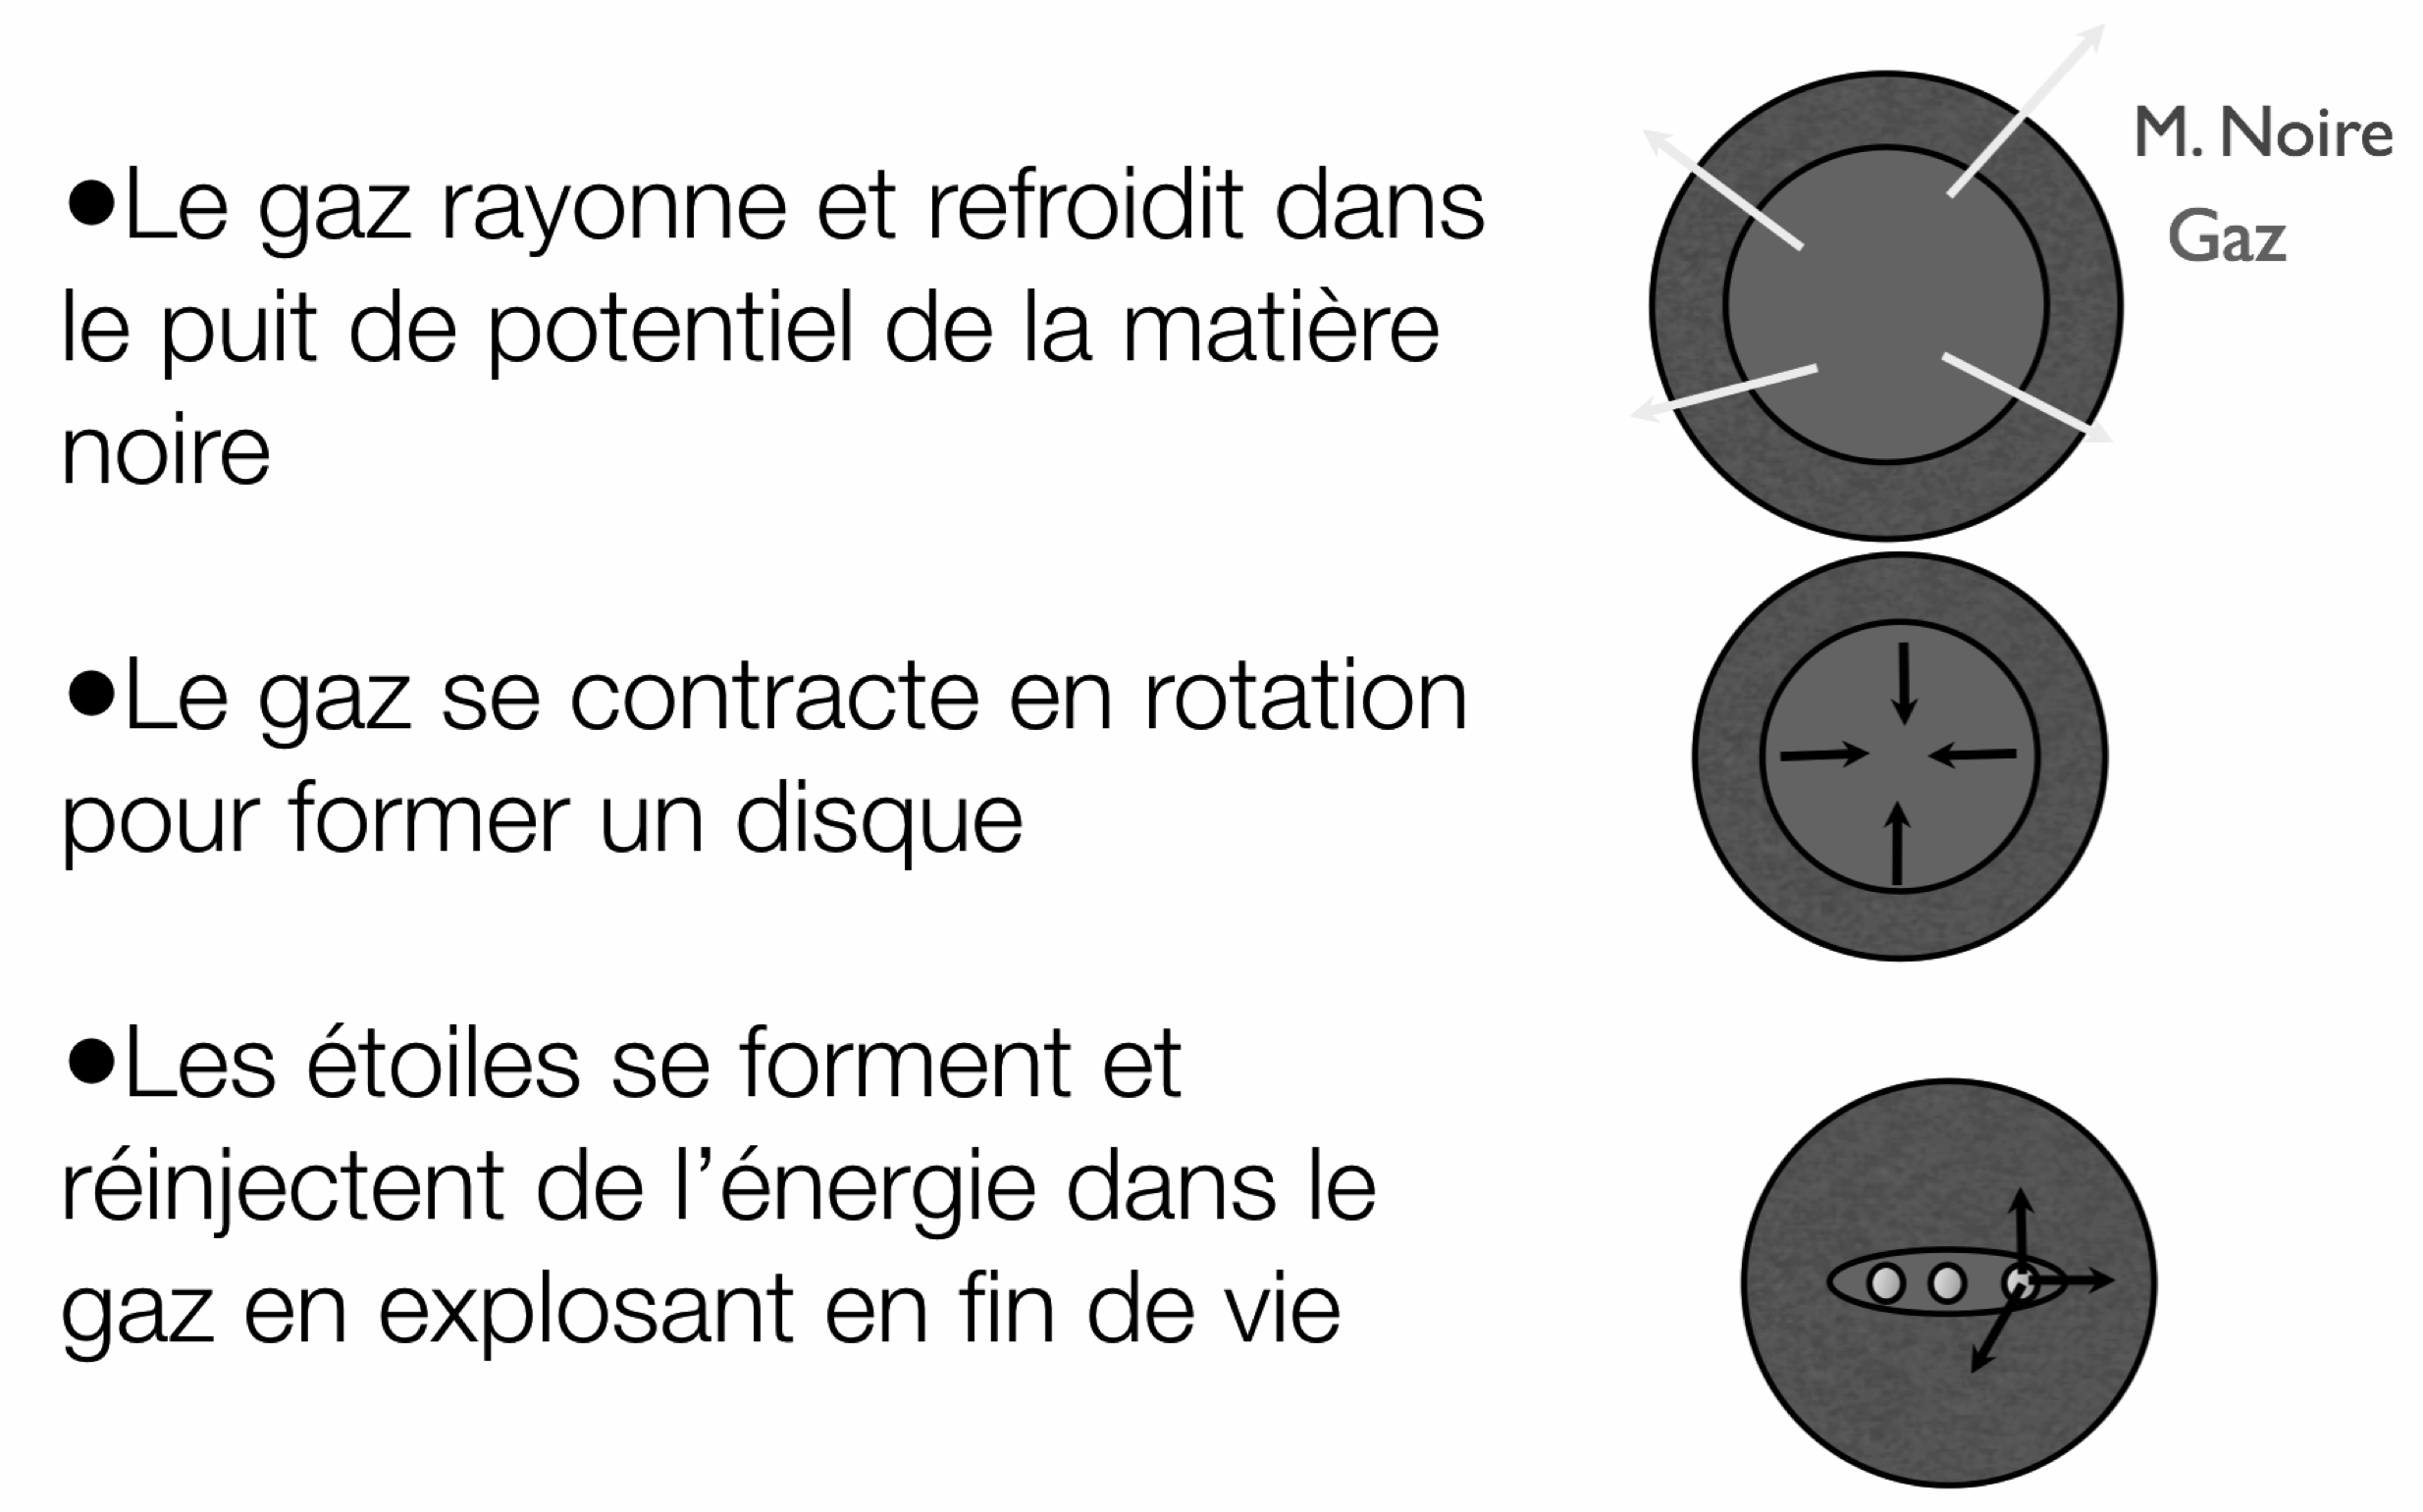
\includegraphics[height=10cm]{figs/coolgal.png}
		\caption[Formation schématique d'une galaxie]{Schéma de la formation d'une galaxie. Dans un premier temps, le gaz évacue de l'énergie interne (refroidissement) dans son halo de matière noire en rayonnant. Ensuite il se contracte pour atteindre des hautes densités : la rotation initiale du gaz est conservée et conduit naturellement à des disques tournants. Enfin, les régimes de densité permettant la formation stellaire se mettent en place dans la galaxie et en fin de vie les étoiles explosent en supernovae et réchauffe le gaz. }
	\label{f:coolgal}
\end{figure}


\newthought{Le gaz n'est pas en reste} dans le processus de viriélisation. Une fois l'équilibre atteint, le gaz va aussi s'organiser dans le potentiel gravitationnel du halo dominé par la matière noire. On peut par exemple lui assigner une température d'équilibre appelée aussi température de viriel\index{température!de viriel}. Conformément au théorème du viriel\index{théorème du viriel}, l'équipartition entre énergie cinétique et potentielle des baryons peut s'écrire:
\begin{equation}
3\frac{M_gk_B T}{\mu m_p} - \alpha \frac{G M_v M_g}{r_v}=0.
\end{equation}
Ici $\mu mp$ désigne la masse typique d'une particule (atome d'hydrogène, hélium, électron), $M_g$ est la masse de gaz totale et $\alpha$ est un facteur de forme proche de l'unité dépendant du profil de masse du gaz. La température de viriel du gaz est donc une fonction simple de la masse et de la taille du halo : $T_v\sim M_v/r_v \sim V_v^2$ \sidenote{ici $V_v=\sqrt{GM_v/r_v}$ désigne la vitesse du Viriel, la vitesse circulaire au rayon de viriel, qui est une mesure de sa masse. }, et pour une masse de halo donné cela implique que si un processus quelconque (comme l'arrivée de rayonnement) chauffe le gaz au dessus de cette température, celui-ci ne peut rester à l'équilibre et éventuellement s'évaporer. Bien sûr la température du gaz à l'intérieur d'une vraie galaxie n'est pas constante et cette température de Viriel n'est qu'une estimation des régimes typiques des températures atteintes au sein des halos.

Toutefois, un gaz dispose d'un canal d'évacuation d'énergie interne inaccessible à la matière noire : les processus baryoniques régis par les interactions électromagnétiques, dont en particulier la production de rayonnement qui peut emporter de l'énergie interne du gaz. On appelle ces processus des \textit{processus de refroidissement}\index{fonction de refroidissement}, caractérisé par une fonction de refroidissement $\Lambda(x,T)$ qui dépend de la température du gaz $T$ et de sa fraction d'ionisation $x$\sidenote{$x=1$ désigne un gaz dont tous les atomes sont ionisés, $x=0$ où ils sont tous neutres}. La quantité d'énergie évacuée par le gaz, en $J/m^3/s$, est donnée par :
\begin{equation}
\Delta e_\mathrm{int}=n_H^2 \Lambda(x,T),
\end{equation}
où $n_H$ désigne la densité d'atomes disponibles.
Cette fonction de refroidissement dicte la quantité d'énergie évacuée à chaque instant par les processus atomiques d'excitation collisionnelle, d'ionisation, de recombinaison et de brehmstrahlung : tous ces processus dépendent du nombre d'atomes neutres et d'électrons disponibles, d'où la dépendance de la fonction de refroidissement en fraction d'ionisation et en $n_H$. Ces processus de refroidissement produisent de la lumière, font diminuer l'énergie interne du gaz qui perd en support thermique et peut donc se contracter davantage : le gaz va devenir de plus en plus dense dans un halo\index{halo} de matière noire qui lui va rester à l'équilibre de viriel. Par ailleurs, la conservation du moment angulaire\index{moment angulaire} du gaz fait que toute rotation initiale de ce dernier, même faible, est maintenue et conduit naturellement à la formation de disques en rotation. 
La conséquence ultime de ce processus de condensation est la formation d'une galaxie et au sein de celle-ci la formation d'étoiles. Bien sûr, si le refroidissement n'est pas assez efficace, le gaz va retrouver son équilibre hydrostatique et l'effondrement du gaz n'aura pas lieu : la compétition entre ces deux effets s'évalue en comparant les temps de refroidissement\index{temps! de refroidissement} et de rééquilibrage\index{temps! de rééquilibrage}
\begin{eqnarray}
t_\mathrm{ref}&\sim &\frac{n_H k_BT}{n_H^2\Lambda}\\
t_\mathrm{eq}&\sim &\frac{1}{\sqrt{G\rho}}.
\end{eqnarray}
On note que le temps d'équilibrage n'est rien d'autre que le temps d'effondrement dynamique\index{temps!dynamique}, qui est le temps typique de réorganisation de la matière sous l'effet de la gravitation. Si $t_\mathrm{eq}\ll t_\mathrm{ref}$ le refroidissement n'est pas assez efficace, l'effondrement baryonique s'arrête. Dans le cas inverse, l'énergie peut être évacuée par rayonnement assez rapidement et la contraction est catastrophique pouvant in fine mener à la formation de galaxie et d'étoiles. On note que le refroidissement varie comme $\rho^{-1}$ tandis que l'équilibrage varie en $\rho^{-1/2}$ : plus le milieu est dense, plus le refroidissement est efficace par rapport à l'équilibrage et favorise ainsi l'effondrement. 

Quand on inspecte rapidement la fonction de refroidissement (voir la figure \ref{f:coolins}), on note celle-ci est maximale pour des températures comprises entre $10^4$ et $10^6$ degrés : en-dessous, les énergies ne sont pas suffisantes pour enclencher les processus atomiques\index{processus atomique}, au dessus le gaz est trop ionisé, limitant les possibilités en termes de processus atomiques disponibles. Par conséquent, les halos trop légers, avec des températures de viriel trop faibles ($M_v<10^9 M_\odot$), ne peuvent refroidir efficacement. De même les objets très lourds ($M_v>10^{13} M_\odot$) présentent en principe les même limitations car possédant des températures caractéristiques trop élevées. En pratique toutefois, les plus gros objets disposent de sous régions denses qui refroidissent efficacement. De même, les plus petits objets bénéficie également de la possibilité de refroidir via les processus \textit{moléculaires}\index{processus moléculaire} du $H_2$ notamment, qui étend les capacités de refroidissement à de plus faibles températures. De même la présence d'éléments plus lourds que l'hélium, désignés sous le terme de métaux\index{métal}, fournit de multiples transitions atomiques et multiplie les canaux d'évacuation de l'énergie : l'enrichissement du gaz par les générations successives d'étoiles favorise le refroidissement du gaz.

\begin{figure}[htbp]
	\centering
		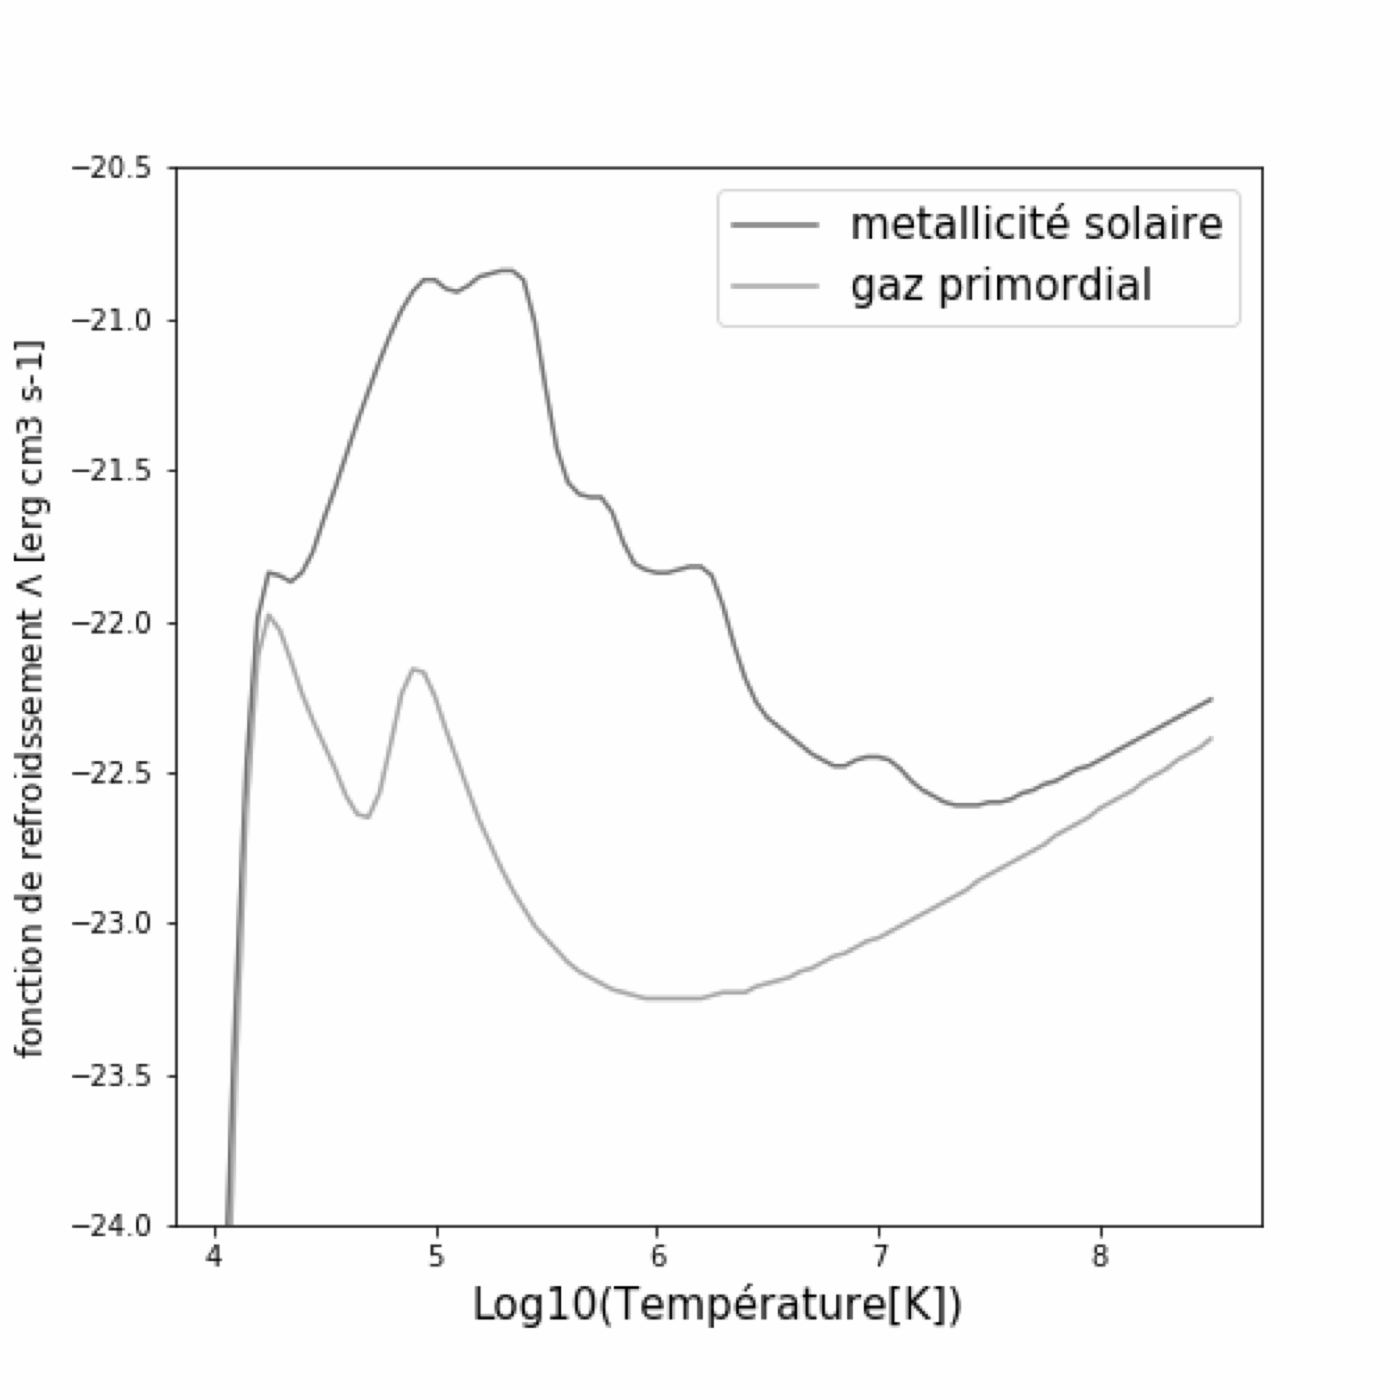
\includegraphics[height=10cm]{figs/cool.png}
		\caption[La fonction de refroidissement du gaz]{La fonction de refroidissement du gaz de Sutherland et Dopita, pour un gaz sans métaux, dit 'primordial' et un gaz avec une métallicité solaire. Dans les 2 cas, le refroidissement n'est efficace qu'au dessus de 10 000 K tandis que les hautes températures présente un comportement en $\sqrt{T}$ typique du Brehmstrahlung. Pour le gaz primordial on observe les 2 'bosses' caractéristiques des processus d'excitation collisionnelle de l'hydrogène et de l'hélium. Le gaz enrichi en métaux est globalement plus efficace car disposant des multiples canaux de refroidissement des éléments plus lourds que l'hélium. Les cas présentés ici suppose un équilibre d'ionisation.}
	\label{f:coolins}
\end{figure}


Pour finir, on a rapidement réalisé que lorsqu'il était actif, ce processus de refroidissement devenait trop efficace en particulier à grand redshift lorsque la matière était très dense, donnant des petites galaxies trop abondantes, un nombre trop important d'étoiles ou des galaxies de tailles trop faible, trop concentrées \sidenote{par exemple dans les travaux de White \& Rees à la fin des années 70 ou Navarro \& White dans les années 90s}. Il faut donc réinjecter de l'énergie dans le gaz pour qu'il arrête ce refroidissement catastrophique, via par exemple l'énergie injectée par les explosions d'étoiles en fin de vie en supernovae\index{supernovae} ou par la présence d'un fond de rayonnement ultra-violet\index{fond UV}. On reviendra sur ces sujets dans la partie dédiée aux simulations numériques.

%\chapter{Simulations Cosmologiques}

\newthought{Cet ouvrage est un ouvrage de théorie}. Il s'agit d'exposer les quantités physiques pertinentes, les temps ou échelles caractéristiques importantes à l'évolution et l'établissement des propriétés de l'Univers : à cette fin, nous posons et analysons les équations que nous croyons pertinentes pour extraire ces informations. C'est une tâche qui généralement ne peut se faire que sous certaines hypothèses dont on sait qu'elle ne sont qu'imparfaitement satisfaites dans la réalité. Par exemple, le principe cosmologique\index{principe cosmologique} présuppose une distribution homogène de la matière or nous savons que cela est n'est plus vrai sur des petites échelles \sidenote{on peut mentionner les oscillations baryoniques acoustiques dans le fond diffus ($\lambda < 200$ Mpc comobile) ou bien la présence d'amas de galaxies dans l'Univers actuel ($\lambda < 1$ Mpc comobile)}.  De même, la théorie de l'instabilité gravitationnelle présentée dans le chapitre sur la formation des structures n'est valable que dans le régime des petites perturbation, autorisant une description linéaire de leur croissance : pour autant nous savons qu'une galaxie présente un contraste de densité $\delta \sim 200$ qui va bien au-delà des limites du régime linéaire. Il existe certes des approches permettant de dépasser le régime des petites perturbations mais elles nécessitent des conditions précises de symétries par exemple \sidenote{tel le modèle d'effondrement sphérique}.


Pour toutes ces raisons, il est tout un domaine de la cosmologie physique qui vise à développer des outils de simulations numériques\index{simulations numériques} permettant notamment de suivre la structuration de la matière dans des régimes arbitraires de symétries et de non linéarités. Ces simulations sont essentiellement dédiées à l'étude de la \textit{dynamique} de la matière dans l'Univers en produisant des portions d'Univers synthétiques en évolution depuis les premiers instants jusqu'à nos jours. Elles reproduisent ce que nous pensons être l'histoire complexe de croissance et d'assemblage des structures : en comparant les prédictions de ces outils à la 'réalité terrain', il s'agit de tester les lois physiques qui sont utilisées et nos hypothèses sur l'état initial de l'Univers et ses propriétés. Par ailleurs ces simulations fournissent des histoires de croissances des structures qui peuvent être enrichies de modèles supplémentaires pour explorer des physiques qui ne se limitent pas à la dynamique. Elles sont aussi utilisées à des fins pratiques pour mettre au point des relevés, préparer des observations ou simuler des instruments. Ces outils numériques sont appelés \textit{simulations cosmologiques} et leurs principes les plus importants sont décrits dans ce chapitre.

\begin{figure}[htbp]
	\centering
		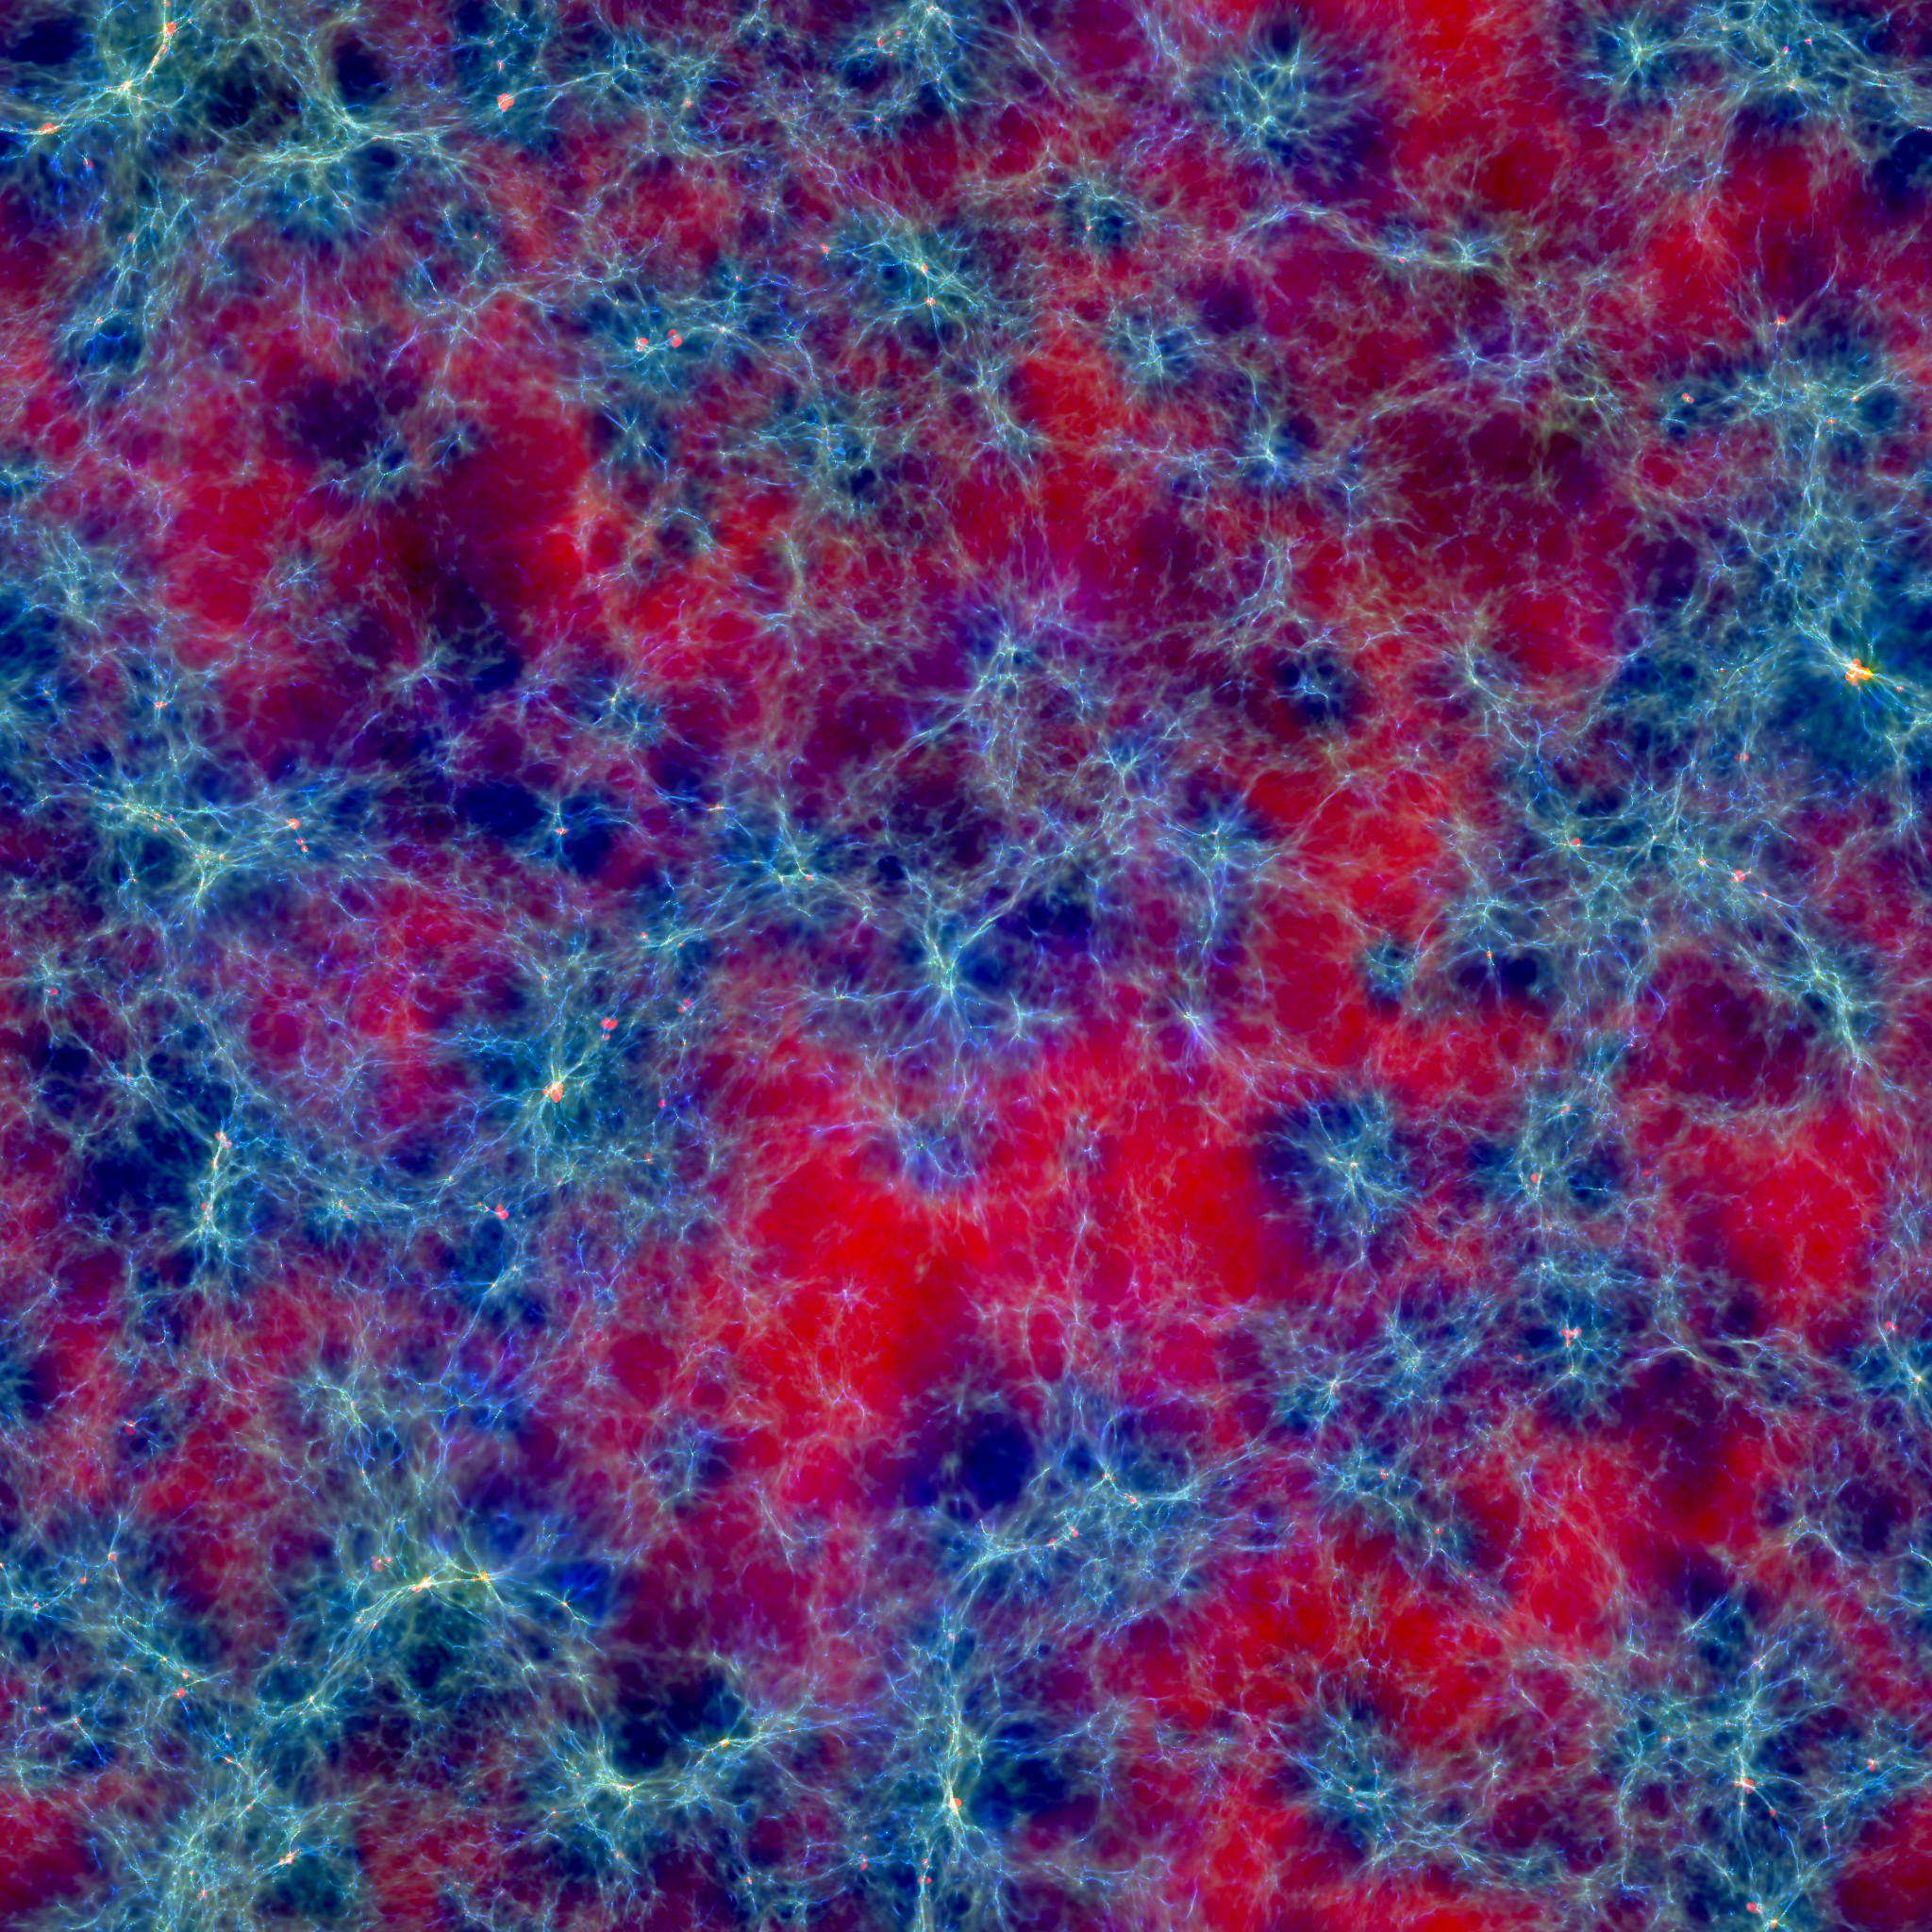
\includegraphics[height=20cm]{figs/simuemma.png}
	\caption[Un exemple de produit de simulation cosmologique]{Un exemple de produit de simulation cosmologique. Cette image montre une prédiction numérique de l'état de l'Univers 1 milliards d'années après le Big-Bang : les structures filamentaires tracent la densité du gaz et le 'brouillard' désigne les régions à température élevée ($>20000$ K). L'image fait 90 Mpc de côté.}
	\label{f:simuemma}
\end{figure}

\section{De la discrétisation et de la résolution}
Ces simulations sont produites par des codes informatiques devant tourner sur des ordinateurs. Ces machines possèdent des ressources finies et manipulent des quantités \textit{discrètes}, ce qui est en contradiction avec notre description habituelle du monde qui repose généralement sur une description \textit{continue} : un volume permet une infinité de positions possibles ou bien tous les instants sont accessibles à l'intérieur d'un intervalle temporel donné. Même une quantité à priori dénombrable peut donner l'apparence d'une infinité, tel un nombre de particules qui dans des volumes cosmologiques peut être tout simplement gigantesque. Un traitement informatique implique donc de discrétiser le temps, l'espace, la distribution de matière, etc... pour pouvoir être envisageable.
Par la suite, nous considérons la densité de matière dans l'espace $\delta(\vec x)$ : ce champ scalaire est défini en tout point de l'espace et possède donc une infinité de valeurs possibles tout en étant mesurable dans une infinité de positions possibles. 

\newthought{Un première façon} de segmenter ce champ consiste à l'évaluer à des positions discrètes, par exemple sur une grille\index{simulations numériques!grille} cartésienne de taille de maille $\Delta x$ : cette façon de faire est dite \textit{eulérienne}\index{eulérienne!discrétisation} et permet de réduire le nombre de points où le champ est évalué tout en lui permettant toujours d'accéder à un spectre continu de valeurs en chacun de ces points. Cette façon de faire introduit en revanche un paramètre de résolution spatiale $\Delta x$ qui va limiter notre capacité à décrire des phénomènes d'échelles caractéristiques proches ou inférieures à cette longueur. On pourra limiter l'influence de ce paramètre de résolution en adoptant par exemple des grilles non cartésiennes, non homogènes ou non statique mais on ne pourra jamais la faire disparaître complètement.

\newthought{Une seconde façon} de procéder consiste à découper la matière en quanta souvent appelés \textit{particules}\index{simulations numériques!particules}, qui représente une quantité prédéfinie de matière se déplaçant librement dans l'espace. Cette description est dite \textit{lagrangienne}\index{lagrangienne!discrétisation} et permet d'accéder à tous les points de l'espace de façon continue. En revanche elle introduit également un élément de résolution, en masse cette fois-ci, correspondant à la masse de la particule $m$ : en un point de l'espace, la quantité matière ne pourra augmenter progressivement depuis zéro qu'en 'empilant' des particules à cet endroit, d'abord $m$ puis $2m,3m$ etc... Par ailleurs cette discrétisation en quanta peut introduire du bruit si une quantité de matière donnée n'est représentée que par un faible nombre de particules. Enfin, comme pour la résolution spatiale mentionnée précédemment, cette résolution en masse nous limite dans la description de phénomènes opérant dans des objets de masse inférieure à cette valeur.

\newthought{Concernant le temps} le même problème se pose: les techniques de résolution approchée d'équations différentielles nécessitent généralement de raisonner sur des durées courtes, par exemple pour satisfaire au mieux des approximations d'ordre linéaire ou de bas ordre. Il faut donc découper les durées d'intérêt en \textit{pas de temps} $\Delta t$ qui à nouveau nous limitent quant à la description de phénomènes plus rapides que cette résolution temporelle. Une simulation numérique tâchera donc de suivre l'évolution de champs discrétisés\index{simulations numériques!discrétisation} sur des grilles (dans une approche eulérienne) ou en particules (dans une approche lagrangienne), en les mettant à jour tous les $\Delta t$ jusqu'à ce que la durée voulue soit couverte. Notons que les 2 approches mentionnées (grille ou particules) possèdent chacune leurs avantages et leurs inconvénients en fonctions des champs considérés et des équations différentielles qui leurs sont associées.


\section{Dynamique Non-Collisionelle: Matière Noire et étoiles}

Considérons dans un premier temps la composante non-collisionnelle de la matière, à savoir la matière noire\index{matière noire} et les étoiles\index{etoiles@étoiles}. Dans la plupart des cas, une simulation cosmologique va décrire ces composantes sous forme de particules possédant une masse $m$, une position $\vec x_i$ et une vitesse $\vec v_i$ ( $i$ désignant la particule parmi N autres). La masse ne varie pas, tandis que positions et vitesses subissent des mises à jour régulières via la résolution du principe fondamental de la dynamique\index{principe fondamental de la dynamique} :
\begin{equation}
\frac{d \vec v_i}{dt}=\frac{1}{m} \vec{F}(\vec x_i)
\end{equation}
où $\vec{F}(\vec x_i)$ désigne la résultante des forces à la position $\vec x_i$. Pour une composante non-collisionelle, cette résultante est uniquement le fruit de la force de gravitation. Un schéma de mise à jour simple peut prendre pour point de départ la discrétisation suivante \sidenote{par la suite on négligera la forme vectorielle des positions et vitesses en se ramenant à un problème 1D. La généralisation à 3D ne posant pas de difficultés.}:
\begin{equation}
\frac{v_i^{p+1}-v_i^{p}}{\Delta t}=\frac{1}{m} {F}(x_i^p)
\end{equation}
et permet d'évaluer la vitesse $v_i^{p+1}$ à l'instant $t^{p+1}=t^p+\Delta t$ comme suit:
\begin{equation}
v_i^{p+1}=v_i^{p}+\frac{\Delta t}{m} {F}(x_i^p).
\end{equation}
Par ailleurs, ayant $dx/dt=v$, on obtient aisément la formule de la mise à jour de la position:
\begin{equation}
x^{p+1}_i=x^{p}_i+\Delta t v_i^{p+1}.
\end{equation}
Ce schéma d'avancement\index{schéma d'avancement} simple est l'une des formes du \textit{schéma d'Euler}\index{schéma d'Euler} : s'il a le mérite de la simplicité, à l'usage il présente des inconvénients en terme de stabilité ou de précision qui nécessitent de manipuler des pas de temps $\Delta t$ particulièrement courts. D'autres schémas plus complexes existent, garantissant une meilleure stabilité ou précision, par exemple le \textit{leapfrog}\index{leapfrog}\sidenote{une traduction possible serait 'saute-mouton'}
\begin{eqnarray}
v_i^{p+1/2}&=&v_i^{p-1/2}+\frac{\Delta t}{m} {F}(x_i^p)\\
x^{p+1}_i&=&x^{p}_i+\Delta t v_i^{p+1/2}
\end{eqnarray}
où l'on voit que vitesse et position sont évaluées de façon désynchronisée avec un décalage de $\Delta t/2$. L'un des mérites de cette méthode est son invariance par renversement du temps \sidenote{on parle de schéma symplectique\index{schéma symplectique}} : en appliquant une mise à jour de $-\Delta t$ le leapfrog permet de retrouver la position $x^p$ à partir de $x^{p+1}$. Le schéma d'Euler ne possède pas la même propriété à cause du terme de force qui passe de ${F}(x_i^p)$ à  ${F}(x_i^{p+1})$ selon qu'on aille dans un sens ou l'autre. 

\newthought{La dernière inconnue} est l'expression de la force en tout point de l'espace ${F}(x_i^p)$. Plusieurs techniques ont été développées depuis les années 70 mais peuvent être rapidement regroupées en 2 familles. La première repose sur un principe de sommation\index{N-Corps!direct}. On dispose des positions $x_i$ de toutes les $N$ particules, on peut donc calculer la force appliquée sur la particule $j$ en sommant toutes les forces individuelles créées par les particules $i$ qui s'appliquent dessus \sidenote{on suppose que toutes les particules sont de masse $m$. $r_{ij}$ désigne la distance entre les particules i et j, tandis que $\vec e_ij $ désigne le vecteur unitaire les reliant} :
\begin{equation}
\vec F_j=-Gm^2\sum_{i\neq j} ^N\frac{1}{r_{ij}^2}\vec e_{ij}. 
\end{equation}
Cette méthode de sommation directe\index{sommation directe} est simple à mettre en place et est rigoureusement exacte, toutefois elle est extrêmement coûteuse puisqu'elle nécessite d'évaluer $N(N-1)/2 \sim N^2$ interactions : si l'on décide de multiplier par 10 le nombre de particules (pour gagner en résolution en masse et étudier de plus petits objets par exemple), cela implique 100 fois plus de calculs. Ce type de dépendance en $N^2$ pour le coût de calcul est tout simplement insoutenable en pratique. Pour cette raison il existe des techniques qui permettent d'accélérer ce type de sommation\index{sommation} par exemple en subdivisant hiérarchiquement l'espace suivant une configuration arborescente\index{N-Corps!arbre}\sidenote{on parle usuellement de \textit{tree-code} ou code en arbre}. Dans ces approches, une région distante (et donc peu influente) est vue avec peu de détails en regroupant les particules qui s'y trouve en 'macro-particules' moins nombreuses, ce qui réduit le cout informatique de la sommation : on peut montrer que le nombre d'interactions suit une loi en $N\log N$, bien plus soutenable. Pour finir, remarquons que la formule de sommation peut diverger si certaines particules sont trop proches l'une des autres avec $r_{ij}\rightarrow 0$ : en pratique il est d'usage de lisser la force de gravitation sur un échelle $\epsilon$. Par exemple on peut écrire
\begin{equation}
\vec F_j=-Gm^2\sum_{i\neq j} ^N\frac{1}{r_{ij}^2+\epsilon^2}\vec e_ij. 
\end{equation}
où $\epsilon$ empêche la force de diverger aux faibles séparations mais au prix d'une réduction de la résolution spatiale : aux échelles de l'ordre du lissage, la force n'est plus correctement décrite.

La seconde famille de méthode pour l'évaluation de la force passe par l'estimation du champ potentiel gravitationnel $\phi(\vec x)$ sur une grille (très généralement) cartésienne\index{simulations numériques!grille}. Force et potentiel\index{potentiel gravitationnel} dérivent l'un de l'autre :
\begin{equation}
\vec F (\vec x) =-\nabla \phi(\vec x)
\end{equation}
tandis que le potentiel peut être évalué en résolvant l'équation de Poisson\index{équation de Poisson@equation de Poisson} à partir du champ de la densité massique $\rho(\vec x)$:
\begin{equation}
\Delta \phi(\vec x) = 4\pi G \rho(\vec x).
\label{e:poissPM}
\end{equation}
Connaissant la position $\vec x_i$ de toutes les particules, on peut évaluer la densité  $\rho(\vec x)$ en tous les points d'une grille\sidenote{en pratique il s'agit de calculer l'histogramme 3D des positions de ces particules} et donc le potentiel $\phi(\vec x)$ puis la force $\vec F(\vec x)$. Connaissant la force en tous les points d'une grille, on peut alors l'interpoler aux positions désirées à savoir les positions $\vec x_i$ de toutes les particules.
\begin{figure}[htbp]
	\centering
		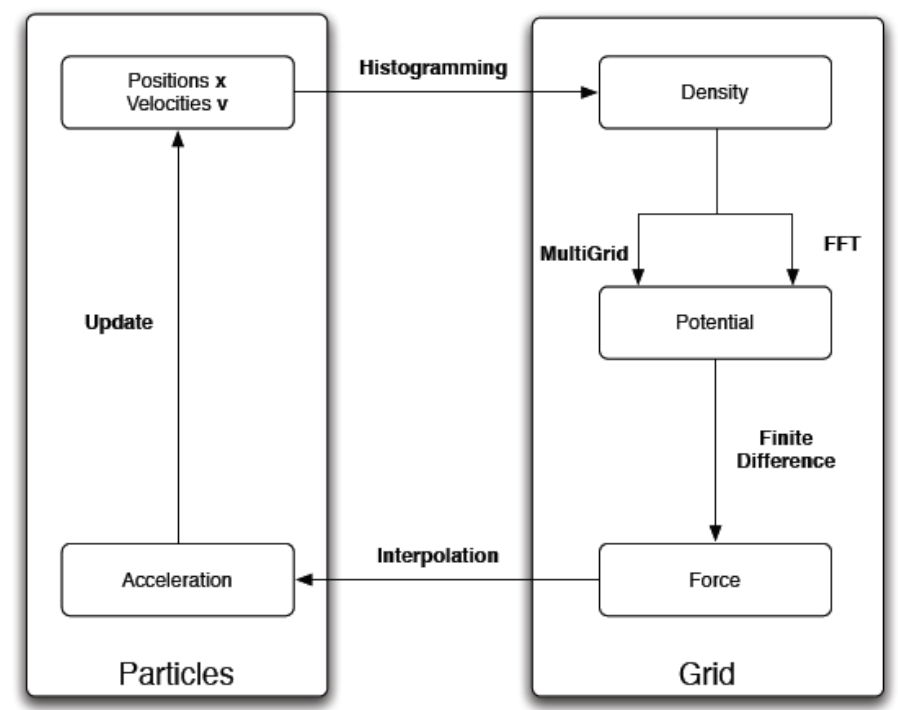
\includegraphics[height=6cm]{figs/PM.png}
	\caption[schématique de la méthode de calcul des forces sur grilles.]{schématique de la méthode de calcul des forces sur grilles. Notez la nature hybride du schéma qui fait intervenir une description en termes de particules (ou lagrangienne à gauche) et une description en termes de champs sur une grille (ou eulérienne à droite)}
	\label{f:PM}
\end{figure}
Pourquoi se donner tant d'efforts pour évaluer la force ou le potentiel de cette façon ? La réponse réside dans la résolution de l'équation de Poisson\index{equation@équations!Poisson} (eq. \ref{e:poissPM}). Cette équation est fondamentalement une équation de diffusion, et nombre de méthodes ont été développée pour la résoudre efficacement et rapidement dans de nombreux contextes. Par exemple, prenons la transformée de Fourier (TF) de l'équation de Poisson et nous obtenons aisément\sidenote{voir aussi le chapitre dédié à la matière noire} : 
\begin{equation}
\tilde \phi(\vec k)\sim -\frac{\tilde \rho(\vec k)}{k^2}.
\end{equation} 
Si nous avons une façon simple d'évaluer les transformées de Fourier de champs connus sur une grille, il suffit d'appliquer l'équation algébrique triviale précédente pour trouver le potentiel à partir de la TF de la densité et du potentiel. Il s'avère qu'il existe des techniques de \textit{transformées de Fourier rapide}\index{transformée de Fourier} ou FFT qui ont été développées durant des décennies à des fins de traitement du signal et qui donc peuvent être facilement reprises. 

Par ailleurs, il existe aussi des méthodes dites de 'relaxation'\index{méthodes de relaxation} qui permettent de résoudre l'équation de Poisson : si on examine cette dernière, on peut considérer qu'elle n'est qu'un cas particulier de l'équation de diffusion
\begin{equation}
\frac{\partial \phi(\vec x,t)}{\partial t}+\Delta \phi(\vec x,t) = 4\pi G \rho(\vec x)
\end{equation}
dans le régime \textit{stationnaire}, avec $\frac{\partial \phi(\vec x,t)}{\partial t}\rightarrow 0$. En cherchant cette solution stationnaire, on peut trouver une solution de l'équation de Poisson. Une version de cette équation en différences finies donne \sidenote{ici $i$ désigne une cellule donc une position dans la grille tandis que $p$ désigne une estimation du potentiel}:
\begin{equation}
\frac{\phi^{p+1}_i-\phi^{p}_i}{\Delta t}+\frac{\phi^{p}_{i+1}-\phi^{p}_{i-1}}{\Delta x^2}=4\pi G\rho^{p}_i
\end{equation}
que l'on peut réarranger sous la forme d'une équation de \textit{relaxation}\index{relaxation}:
\begin{equation}
\phi^{p+1}_i=\phi^{p}_i+4\pi G\rho^{p}_i-\frac{\phi^{p}_{i+1}-\phi^{p}_{i-1}}{\Delta x^2}\Delta t.
\end{equation}
En se donnant une estimation du potentiel $\phi^{p}_i$ à une itération $p$ et en l'utilisant dans cette relation de relaxation, on s'approche en principe d'une estimation encore meilleure $\phi^{p+1}_i$. D'itérations en itérations, on peut ainsi converger vers une solution du potentiel : notons que l'on utilise un pas de temps \textit{fictif} $\Delta t$ dont on peut montrer qu'une convergence optimale est obtenue pour $\Delta t\sim \Delta x^2/2$. La méthode décrite ici est la plus simple de toutes les méthodes de relaxation \sidenote{c'est la méthode de \textit{Jacobi}\index{méthode de Jacobi}}: il en existe d'autres, plus stables, plus efficaces dont les méthodes dites \textit{multigrilles} qui cherchent à faire converger les différentes échelles du potentiel de façon séparées et optimales. Comparées au méthodes à base de FFT, elles sont plus versatiles\sidenote{on peut aussi les utiliser pour des versions modifiées de l'équation de Poisson ou sur des grilles non cartésiennes} et légèrement moins rapides.

Que ce soit grâce à la FFT ou aux méthodes de relaxation, on dispose de moyens extrêmement rapides de résolution de l'équation de Poisson : en revanche l'utilisation d'une grille implique que le champ de gravitation n'est décrit qu'au mieux sur une échelle de la taille d'une cellule de la grille. Une telle échelle de coupure est inexistante à priori dans les méthodes de sommation qui permettent donc un suivi plus précis et à plus petite échelles des effondrements par exemple. L'introduction d'un lissage $\epsilon$ dans les méthodes de sommation introduisent certes une résolution limite mais ce lissage est généralement bien plus petit que la taille d'une cellule (environ 10 fois plus petit en pratique). De fait, on n'hésite pas parfois à combiner les méthodes de sommation et celles de type grille pour bénéficier de leurs avantages respectifs.

Pour finir, considérons rapidement la différence entre particules de matière noire\index{matière noire} et étoiles\index{etoiles@étoiles}, qui toutes deux sont l'objet de la dynamique non-collisionnelle. Dans les 2 cas, les méthodes exposées ici sont appliquées de façon identiques, les deux espèces diffèrent en ce que leurs membres n'évoluent pas de la même manière. Les particules de matières noires n'évoluent pas, leur masse individuelle reste constante, leur nombre initial fixe la quantité de matière noire et il n'a pas d'annihilation ni de création de telles particules. Les étoiles évoluent: elles doivent apparaître lorsque les conditions s'y prêtent et elles peuvent voir leur masse évoluer : en effet une particule 'stellaire' constitue en pratique un amas stellaire  de plusieurs centaines d'étoiles à plusieurs millions de masse solaires. Elles représentent donc davantage une population qu'une étoile individuelle en tant que tel : lorsque les étoiles les plus massives de ces amas explosent en supernovæ\index{supernovæ}, la masse est rendue au milieu interstellaire au bout de quelques millions d'années et numériquement cela peut correspondre à une masse variable de particule. Notons toutefois qu'il existe toujours au sein de ces particules stellaire une composante 'étoile de faible masse' à durée vie supérieure au temps de Hubble: de façon générale une particule stellaire voit sa masse diminuer mais ne peut complètement disparaître du fait de cette population à grande durée de vie.

\section{Hydrodynamique}
\newthought{En contrepoint} à la dynamique non-collisionnelle, les codes de simulations numériques peuvent également suivre la dynamique du gaz\index{hydrodynamique} présent dans l'Univers. Ces baryons ne représentent certes que $\sim 15\%$ de la matière disponible mais ils sont observables ou bien sont à l'origine des étoiles qui sont également observables : par conséquent ils permettent une comparaison plus directe des résultats simulés aux observations. Par ailleurs au centre des galaxies, le gaz peut être dominant et sa dynamique est suffisamment différente de celle de la matière noire et des étoiles pour devoir être modélisée indépendamment.

\newthought{Le jeu d'équation} à résoudre est connu, ce sont les équations d'Euler\index{equation@équations!Euler}\sidenote{représentées ici à 1D. On y distingue l'équation de la conservation de la masse et de l'impulsion. $\rho(x,t)$ désigne la densité de gaz, $v(x,t)$ sa vitesse, $P(x,t)$ sa pression\index{pression} et $\phi(x,t)$ le potentiel gravitationnel.}:
\begin{eqnarray}
\frac{\partial \rho}{\partial t}+\frac{(\partial \rho v)}{\partial x}&=&0\\
\frac{\partial v}{\partial t} + v \frac{\partial v}{\partial x}&=&-\frac{1}{\rho}\frac{\partial P}{\partial x}-\frac{\partial \phi}{\partial x}
\end{eqnarray}
La première équation indique que la densité ne varie que sous l'effet du flux de masse ($\frac{(\partial \rho v)}{\partial x}$) tandis que la seconde indique que l'impulsion varie sous l'effet du flux de moment ($ v \frac{\partial v}{\partial x}$) et des forces de pression ($\frac{\partial P}{\partial x}$)  et de gravitation ($\frac{\partial \phi}{\partial x}$) \sidenote{il s'agit juste d'une formulation alternative du principe fondamental de la dynamique}.

Ces équations peuvent être toutes deux écrites sous une forme \textit{conservative}\index{equation@équation de conservation}
\begin{eqnarray}
\frac{\partial \rho}{\partial t}+\frac{(\partial \rho v)}{\partial x}&=&0\\
\frac{\partial \rho v}{\partial t}+\frac{(\partial \rho v v)}{\partial x}&=&-\frac{\partial P}{\partial x}-\frac{\partial \phi}{\partial x}\\
\frac{\partial E}{\partial t}+\frac{(\partial E v)}{\partial x}&=&-v \frac{\partial P}{\partial x}-v\frac{\partial \phi}{\partial x}
\end{eqnarray}
auxquelles nous avons ajouté l'équation de conservation\index{equation@équations!conservation} de l'énergie $E$. Ces 3 équations suivent une structure similaire, typique d'équations de conservation d'une quantité $A$ avec un terme source\index{terme source}
\begin{equation}
\frac{\partial A}{\partial t}+\frac{\partial F(A)}{\partial x}=S(A).
\label{e:cons}
\end{equation}
Dans les 3 cas, une quantité $A$ est modifiée sous l'effet d'un flux $F(A)$, qui déplace la quantité en question, et d'un terme source qui modifie $A$ sans déplacement. Dans le cas de la densité, ce terme source est strictement nul ce qui indique une conservation stricte de la masse, dans le cas de l'impulsion, ce terme source est constitué des forces qui s'exercent sur le fluide et dans le cas de l'énergie il est finalement constitué du travail de ces même forces.

La façon la 'plus naturelle' de résoudre des équations du type de Eq. \ref{e:cons} est de considérer un volume fini\index{volumes finis}, comme celui d'une cellule cubique et de mesurer les flux des quantités conservées (densité, impulsion et énergie) au travers des faces de cette cellule. Intuitivement, le flux mesuré au travers d'une face dépend des valeurs physiques de part et d'autre de cette face : la procédure qui permet de trouver le flux de $A$ connaissant $A$ de part et d'autre de l'interface s'appelle une \textit{résolution de problème de Riemann}\index{problème de Riemann}.

 Il existe nombre de façons de résoudre un problème de Riemann, avec des niveaux d'approximations plus ou moins importants. Soit par exemple $F(A_{i+1/2})$, le flux existant entre 2 cellules successives $i$ et $i+1$ : résoudre le problème de Riemann revient à trouver la fonction $\mathcal R$ telle que
 \begin{equation}
 A_{i+1/2}=\mathcal{R}(A_i, A_{i+1/2}).
 \end{equation}
 Une façon simple de procéder revient à comparer les 'vents' dans les cellules adjacentes en comparant leurs vitesses: si $v_i>v_{i+1}$ le vent vient de la cellule $i$ et on peut considérer que la valeur de $A$ à l'interface est dominée par $A_i$. Cette procédure dite \textit{upwind} va par exemple assigner:
  \begin{equation}
 A_{i+1/2}=\mathcal{R}(A_i, A_{i+1/2})\sim A_i
 \end{equation}
 et donc $F(A_{i+1/2})\sim F(A_{i})$. On peut toutefois montrer que ce type de schéma est soit extrêmement diffusif soit particulière instable et il existe toute une littérature de schémas de plus haut niveau, plus ou moins adaptés en fonction du problème que l'on cherche à résoudre.
 
 Connaissant le flux\index{flux} en $i-1/2$ et $i+1/2$, la quantité $A$ peut être mise à jour par le même type de différence finie que celle utilisée précédemment pour le déplacement de particule non-collisionelle :
 \begin{equation}
 \frac{A_i^{^p+1}-A_i^p}{\Delta t}=-\frac{F(A_{i+1/2}^p)-F(A_{i-1/2}^p)}{\Delta X}+S(A_i^p)
 \end{equation}
 ou bien
 \begin{equation}
 A_i^{^p+1}=A_i^p-\Delta t \frac{F(A_{i+1/2}^p)-F(A_{i-1/2}^p)}{\Delta X}+\Delta t S(A_i^p).
 \end{equation}
Notez que cette mise à jour à l'instant $p+1$ ne nécessite la connaissance que des données à l'instant $p$ et tous les termes du membre de droite sont évalués à cet instant. Cette approche est dite \textit{explicite}\index{schéma explicite} et n'est que conditionnellement stable. Si le pas de temps $\Delta t$ est trop important, une amplification des erreurs s'opère et la stabilité n'est garantie que si la condition de Courant est satisfaite :
\begin{equation}
\frac{\Delta x}{ \Delta t}> v.
\end{equation}
Cette équation traduit que la vitesse numérique, la vitesse de mise à jour, doit être supérieure à la vitesse typique du processus physique que l'on cherche à reproduire : pour une résolution spatiale $\Delta x$ donnée cela équivaut à mettre une limite supérieure au pas de temps $\Delta t$ choisi \sidenote{Notons que la même chose existe pour les particules de la partie précédente. Si l'on souhaite qu'une particule ne parcoure pas une trop grande distance durant un pas de temps, il faut limiter ce dernier.} Notons qu'il existe aussi une approche dite \textit{implicite}\index{schéma implicite} où tous les termes de mise à jour sont exprimés à l'instant $p+1$ : toutefois ces termes sont inconnus au moment du calcul et la mise à jour implique dès lors un problème typique d'inversion, souvent compliqué, en lieu et place de la simple expression algébrique obtenue ici. En revanche l'approche implicite est généralement inconditionnellement stable, ce qui permet l'utilisation de pas de temps plus grands pour simuler un problème donné.

\newthought{Une autre méthode populaire} existe pour traiter les équations hydrodynamique et qui repose sur une description particulaire des éléments de fluides. Nommée \textit{SPH} (pour \textit{smoothed particle hydrodynamics})\index{SPH} elle repose sur l'utilisation de particules d'extension finie et non-nulle. Cette extension est formalisée par un noyau dont la valeur dépend de la distance au centre de la particule, $W(|x-x_p|)$, valeur qui tend vers zéro au delà d'une certaine \textit{distance de lissage}. Ce noyau fait office de poids et toute quantité intensive (densité, moment, énergie...) associée à une particule s'obtient en additionnant les contributions pondérées de ses $i$ voisines:
\begin{equation}
A=\sum_i m_i \frac{A_i}{\rho_i} W(|x_i-x_p|).
\end{equation} 
Cette somme se fait généralement sur un nombre de particules voisines prédéterminé : si la matière est dense, les distances impliquées seront courtes tandis qu'un état diffus implique naturellement une sommation sur des plus grandes distances.
 
L'intérêt de cette méthode est sa simplicité : par exemple toute dérivée spatiale de $A$ se propage linéairement au noyau de pondération, dont la dérivée est généralement simple et connue. De plus, cette description sous forme de particule n'implique pas de géométrie d'échantillonnage à priori, au contraire d'une grille qui fixe d'emblée des directions ou des points de mesures privilégiés. Les particules de fluides se déplacent librement et peuvent par exemple sur-échantillonner les régions denses ou sous échantillonner les régions vides : par rapport à une grille, on a ainsi un échantillonnage de l'espace au plus près des contrastes de densité. Son inconvénient majeur est sa plus grande diffusivité comparées aux meilleures formulations sur grille : dans ses versions les plus communes, la méthode SPH ne parvient pas à capturer certains types chocs ou de discontinuités et ne lui permet pas de reproduire certaines instabilités hydrodynamiques standard. 

\begin{figure}[htbp]
	\centering
		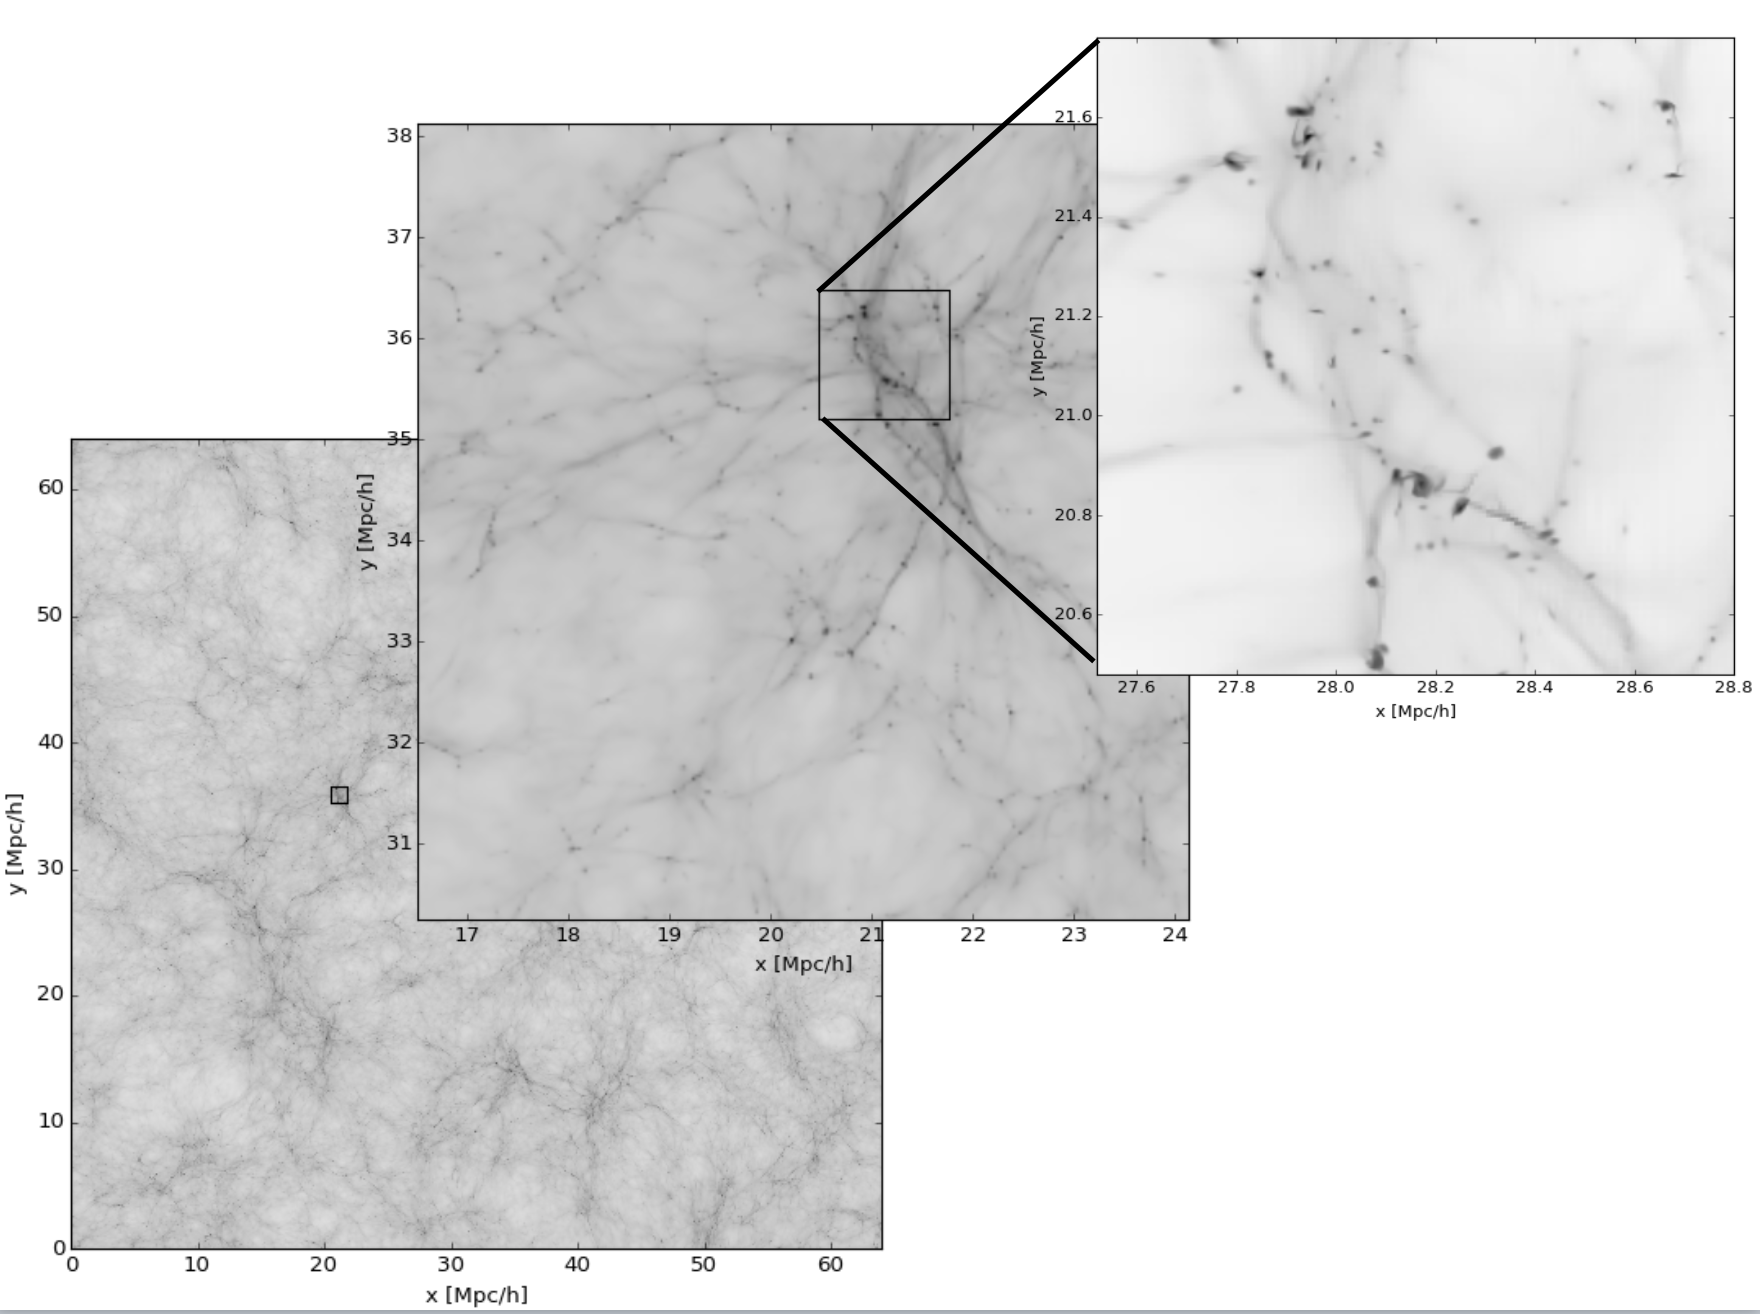
\includegraphics[height=12cm]{figs/zoom.png}
	\caption[Exemple de dynamique dans une simulation hydrodynamique avec refroidissement.]{Exemple de dynamique dans une simulation hydrodynamique avec refroidissement. L'image de droite représente la distribution de gaz dans les 2 cadres de gauches. On note la présence de disques gazeux en rotation créés par le gaz effondré sous l'effet du refroidissement.}
	\label{f:zoom}
\end{figure}


\section{Processus Physico-Chimiques}
Comme expliqué dans la partie dédiée à la formation des structures, le gaz cosmique ne peut s'organiser sous la forme de galaxies que si ce dernier peut évacuer de l'énergie via des processus de refroidissement\index{refroidissement}. L'équation qui régit l'évolution de l'énergie interne\index{energie@énergie interne} est\sidenote{$e$ désigne l'énergie interne du gaz tandis que $H$ et $\Lambda$ désignent respectivement les fonctions de chauffage et de refroidissement} :
\begin{equation}
\frac{de}{dt}=H-\Lambda.
\end{equation}
La fonction de chauffage\index{chauffage} $H$ est régie par le rayonnement ionisant. La fonction de refroidissement $\Lambda$\index{fonction de refroidissement} peut être plus ou moins sophistiquée et faire intervenir des espèces moléculaires, des métaux \sidenote{éléments plus lourds que l'hélium} ou se limiter aux éléments H\index{hydrogène} et He\index{hélium}. Dans ce dernier cas, les processus impliqués sont le refroidissement par ionisation, par émission de rayonnement de recombinaison, de désexcitation collisionelle ainsi que le rayonnement synchrotron\index{synchrotron} et Compton\index{Compton} inverse avec les photons du CMB\index{fond diffus cosmologique}. Tous ces processus sont tabulés et dépendent de la température du gaz, de sa densité et de son état d'ionisation. 

\newthought{L'état d'ionisation du gaz}\index{ionisation} doit également être connu pour chaque élément de résolution afin de calculer son refroidissement. Dans le cas d'un gaz composé uniquement d'hydrogène, l'état d'ionisation du gaz est régi par \sidenote{$n_{HI}$ désigne la densité numérique de gaz d'hydrogène neutre, $n_{HII}$ celle d'hydrogène ionisé et $n_e$ la densité d'électrons libres }:
\begin{equation}
\frac{dn_{HI}}{dt}=\alpha(T) n_{HII} n_e-\beta(T) n_{HI}n_e-\Gamma n_{HI}.
\label{e:eint}
\end{equation}
Cette équation lie la variation de l'abondance d'atomes neutres à la recombinaison atomique\index{recombinaison} \sidenote{contrôlée par le taux de recombinaison $\alpha$ (en $m^3 s^{-1}$)} qui tend à faire augmenter cette abondance en fonction du nombre d'électrons libres et d'atomes ionisés, à l'ionisation collisionelle \sidenote{contrôlée par le taux de collisions $\beta$ (en $m^3 s^{-1}$)} qui tend à diminuer cette abondance en fonction du nombre d'électrons libres à nouveau et enfin par la photoionisation\index{photoionisation} \sidenote{contrôlée par le taux de photoionisation $\Gamma=c\sigma n_\gamma$ (en $s^{-1}$)} qui encode la destruction d'atomes neutres par le rayonnement ionisant. Ce type d'équation doit être résolue en chaque élément de résolution à chaque pas de temps. Elle peut être résolue dans le régime hors-équilibre \index{chimie!hors-équilibre} ou plus simplement en supposant que cette abondance converge très rapidement vers l'équilibre\index{chimie!à l'équilibre}\sidenote{ce qui est une bonne approximation compte tenu des temps courts impliqués dans les processus physico-chimiques par rapports aux temps dynamiques} en posant arbitrairement $\frac{dn_{HI}}{dt}=0$.

\newthought{Les taux} physico-chimiques de recombinaison ou de collisions dépendent uniquement de la température\index{température} et sont tabulés. Le taux de photoionisation dépend lui de la quantité de photons $n_\gamma$ ionisants présents en chaque point de l'espace simulé\sidenote{$\sigma$ désigne la section efficace d'ionisation\index{section efficace!d'ionisation} et dépends très fortement de la fréquence du rayonnement étudié.}:
\begin{equation}
\Gamma=c\sigma n_\gamma.
\label{e:photoion}
\end{equation}
Ce rayonnement ionisant\index{ionisation} est produit par les étoiles\index{etoiles@étoiles} et les quasars\index{quasars} pour l'essentiel et dépend dans l'absolu du lieu considéré (à proximité ou éloigné des sources de rayonnement) et de l'instant puisque les populations d'étoiles et de quasars évoluent au cours de l'histoire de l'Univers. En pratique, la plupart des simulations cosmologiques considère que le rayonnement ionisant est assimilable à un fond uniforme\index{fond UV}~: après la Réionisation\index{Réionisation}\sidenote{qui prend place environ 1 milliard d'années après le Big-Bang, correspondant à $z\sim 6$.}, l'Univers est 'transparent' aux rayonnements UV et cela constitue donc une approximation raisonnable. L'évolution temporelle de ce 'fond UV'\index{fond UV} peut être tabulé et injecté dans l'équation \ref{e:photoion}. Un exemple couramment utilisé est le fond dit de 'Haardt \& Madau', reposant sur une description réaliste de l'évolution des différentes populations de sources et dont l'évolution est donnée dans la figure \ref{f:HM}. Ce taux intervient également dans le terme de chauffage $H$\index{chauffage} de l'équation \ref{e:eint} : chaque ionisation\index{ionisation} s'accompagne d'un dépôt d'énergie de la forme \sidenote{où $E_\gamma$ désigne l'énergie portée par chaque photon et $E_i$ désigne l'énergie d'ionisation (13.6 eV pour H)}:
\begin{equation}
H=c \sigma n_\gamma n_{HI} (E_\gamma-E_i).
\end{equation}
Donc non seulement le rayonnement influe sur le refroidissement du gaz en réglant le taux d'ionisation du gaz (et donc sa capacité à rayonner) mais également sur son chauffage. Depuis un peu moins de 10 ans, un nouveau type de simulations prenant en compte la propagation du rayonnement et les effets d'opacités \sidenote{physique que l'on regroupe sous le terme de \textit{transfert radiatif}\index{transfert radiatif}} est apparu : extrêmement coûteuses ces simulations sont pour l'instant limitées à l'étude de l'époque de Réionisation\sidenote{donc limité au premier milliard d'années de l'histoire de l'Univers} mais permettent de s'affranchir de l'hypothèse d'un fond UV uniforme. 

\begin{figure}[htbp]
	\centering
		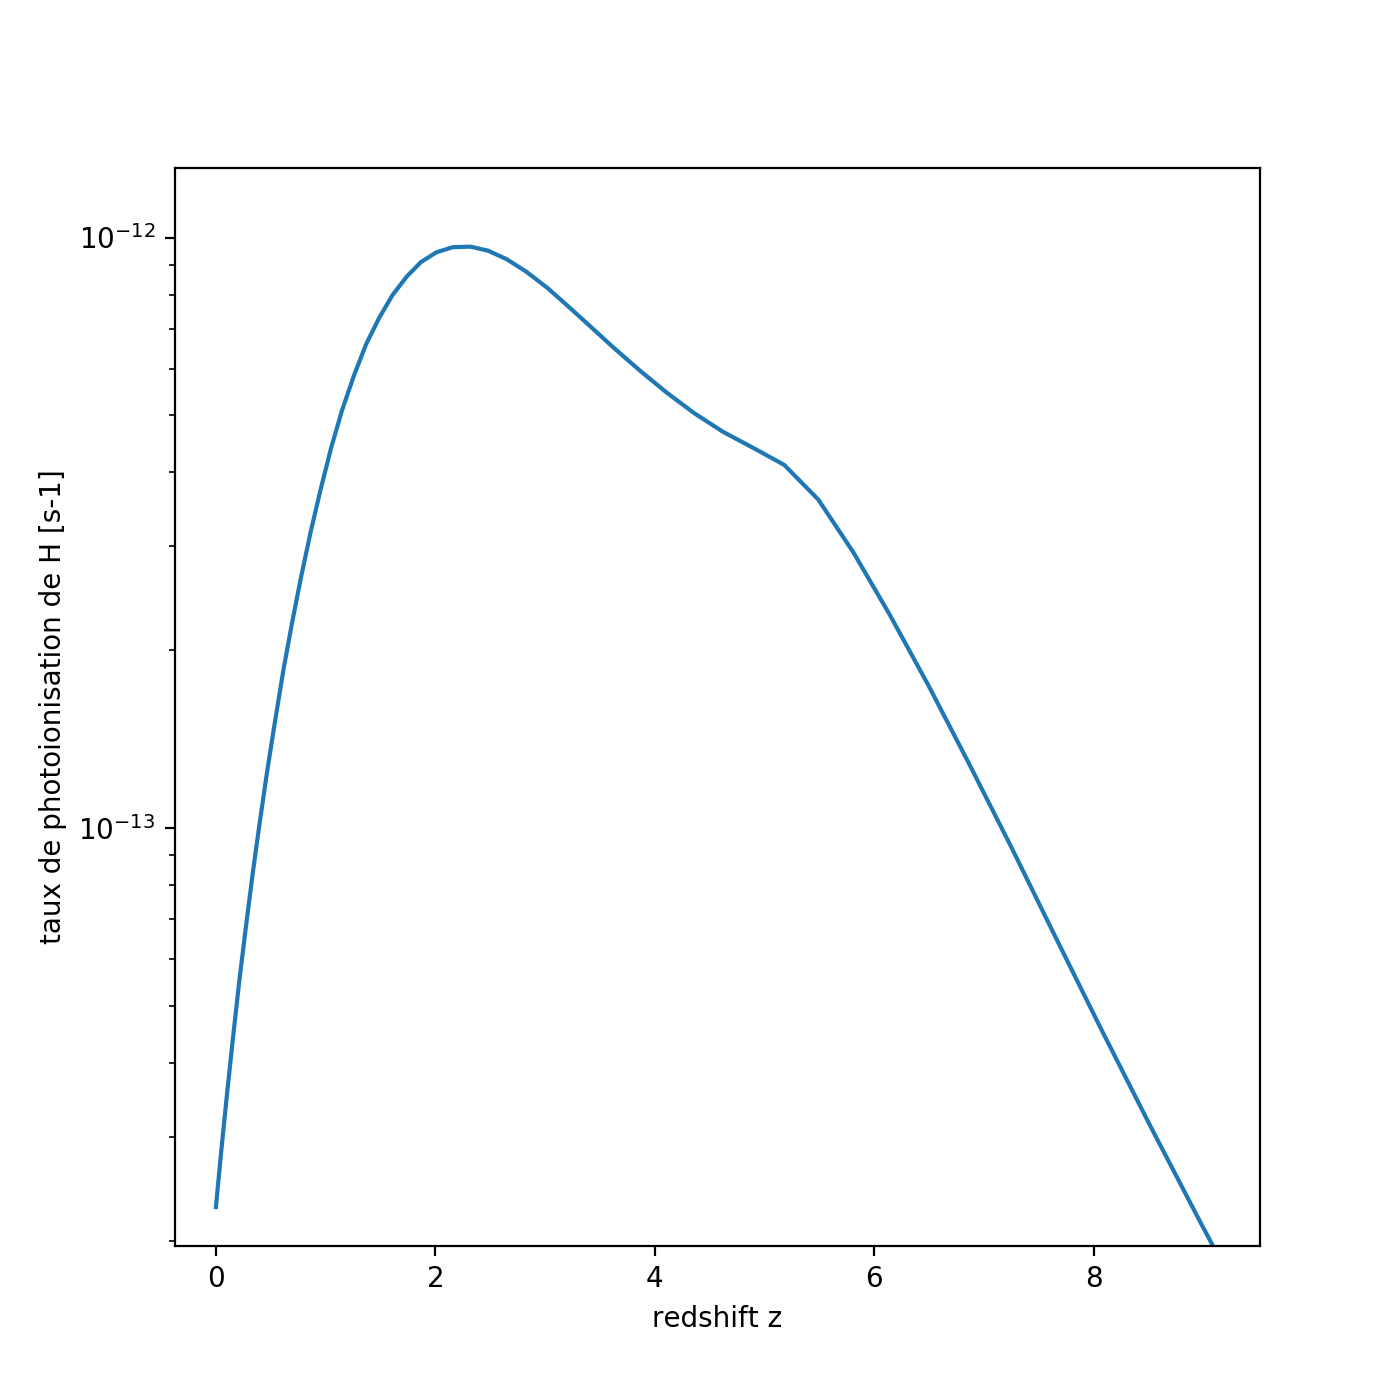
\includegraphics[height=12cm]{figs/HM.png}
	\caption[modèle de Haardt \& Madau]{Évolution en redshift du taux de photoionisation crée par le fond ultra-violet du modèle de Haardt \& Madau. Ce modèle suppose un Univers optiquement mince et sort de son domaine d'hypothèse pour z>6, lorsque l'Univers n'est pas complètement réionisé. On note une augmentation suivi d'une baisse du taux de photoionisation qui trace l'histoire cosmique de formation d'étoile.}
	\label{f:HM}
\end{figure}


\section{Formation et rétroaction stellaire}
L'objectif des simulations cosmologiques est d'explorer le processus de croissances des structures dans ses régimes les plus non-linéaires et l'un des aboutissement de ces régimes est la formation d'étoile\index{etoiles@étoiles!formation}. Par ailleurs, la comparaison entre résultats de modélisation et observations se fait invariablement par la composante lumineuse des galaxies et à ce titre l'inclusion de modèles de formation stellaire est indispensable pour pouvoir comparer une vraie galaxie avec la composante stellaire d'une galaxie simulée.

\newthought{La résolution spatiale}\index{simulations numérique!résolution} nécessaire à modéliser la formation stellaire est néanmoins difficilement compatible avec les échelles cosmologiques. La formation stellaire opère dans des nuages moléculaires géants\index{nuage moléculaire}, aux tailles caractéristiques de l'ordre du parsec, tandis que les effets cosmologiques qui nous intéressent se manifestent sur des échelles supérieures au Mégaparsec : le rapport d'échelle est très important et à vrai dire hors de portée des machines actuelles de calcul. En effet, une haute résolution spatiale dans un grand volume cosmologique implique un grand nombre d'éléments de calculs (particules, cellules) et donc un grand nombre de données à traiter sur une très grande durée. Par exemple, un volume de 100 Mpc traité avec des cellules au parsec de résolution implique un nombre de cellules total de l'ordre de $(10^8)^3=10^{24}$. En 2017, les plus grandes simulations cosmologiques produites sur les plus grands calculateurs mondiaux traitent avec difficulté de problèmes échantillonnés sur $10^{11-12}$ cellules, bien en deçà de l'exigence que nous venons de formuler.

\newthought{La formation stellaire}\index{etoiles@étoiles!formation} ne peut donc être simulée à partir de 'principes premiers'\sidenote{dans des volumes cosmologiques. Il existe des simulations à l'échelle du nuage moléculaires qui ont la résolution suffisante mais qui se restreignent à des volumes physiques simulés bien insuffisants pour faire de la cosmologie.} et il faut donc avoir recours à des modèles. Une des approches les plus communes repose sur l'idée que la formation stellaire est régie par l'effondrement gravitationnel du gaz et opère donc sur des temps dynamiques\index{temps!dynamique} \sidenote{$\rho_*$ désigne la densité de masse stellaire formée, $\rho_g$ désigne la densité de gaz convertie en étoile et $t_g$ est le temps dynamique gravitationnel}:
\begin{equation}
\frac{d \rho_*}{dt}=\frac{d \rho_g}{dt}\sim\epsilon\frac{\rho_g}{t_g}.
\end{equation}
Ici $\epsilon$ désigne l'efficacité de formation stellaire et manifeste le fait que le temps caractéristique de formation d'étoile n'est pas exactement le temps dynamique mais plutôt $t_g/\epsilon$ : l'efficacité est un paramètre libre du modèle.

Or le temps dynamique\index{temps!dynamique} est lui même dépendant de la densité de gaz en effondrement:
\begin{equation}
t_g\sim\frac{1}{\sqrt{G\rho_g}}.
\end{equation}
Le taux de formation stellaire\index{taux de formation stellaire} (SFR \sidenote{de l'anglais \textit{Star Formation Rate}}) est alors décrit par une loi de puissance sur la densité de gaz présente localement:
\begin{equation}
\mathrm{SFR}\sim \epsilon \rho_g^{3/2}.
\label{e:schmidt}
\end{equation}
Cette relation est appelée \textit{Loi de Schmidt}\index{loi de Schmidt} et traduit en des termes simples qu'une région dense et riche en gaz produit naturellement plus d'étoiles : l'efficacité du processus est contrôlée par $\epsilon$ et opère sur des échelles de temps $t_g/\epsilon$. Observationnellement, on constate toutefois que le processus de formation stellaire est hautement inefficace avec des temps caractéristiques de conversion de l'ordre de quelques milliards d'années alors que les temps d'effondrement attendus sont environs 100 fois plus courts. L'efficacité de formation stellaire\index{efficacité de formation stellaire} est donc de l'ordre de $1\%$ et traduit l'impact macroscopique de processus non résolus qui empêche une formation d'étoile soutenue\sidenote{on ne connaît pas bien la source précise de cette inefficacité. Champs magnétiques, turbulence, vents stellaires sont souvent invoqués sans que leurs rôles relatifs et quantitatifs ne soient exactement connus.}.

\newthought{En pratique}, un code de simulation va passer en revue tous ses éléments de résolution et convertir une partie du gaz conformément à la Loi de Schmidt\index{loi de Schmidt}. Cette conversion va se manifester sous la forme de création de particules stellaires : ces particules n'interagissent que via la gravitation et se découplent du gaz comme de vrais étoiles. Ces "étoiles" possèdent un âge, éventuellement une composition chimique synthétique qui permet de leur assigner une luminosité ou un spectre pouvant amener des comparaisons entre ces populations stellaires simulées et celles observées dans les vraies galaxies. Rappelons pour finir que ces particules stellaires ont des masses typiques de l'ordre de 1000 $M_\odot$ à quelque millions et représentent donc des amas ou des populations stellaires et non pas des étoiles individuelles : nos machines actuelles ne sont pas capables de gérer le nombre réel d'étoiles présentes dans un volume cosmologique et doivent donc les regrouper en 'macro-étoiles'.

\newthought{Une étoile meurt}, parfois de façon spectaculaire si elle est massive, de l'ordre de la dizaine de masses solaire ou plus. Cette mort s'accompagne d'une explosion en supernova\index{supernova} qui va injecter de l'énergie dans le gaz environnant, le chauffer et donc prévenir au moins momentanément l'apparition de génération ultérieures d'étoiles (voir Fig. \ref{f:SN}). Une population existante va donc modérer l'apparition de populations suivantes dans un mécanisme de rétroaction\index{rétroaction}\sidenote{en anglais on parle aussi de \textit{feedback}}. Les codes de simulations vont modéliser cette rétroaction en injectant de l'énergie dans le gaz à proximité des particules stellaires qui atteignent l'âge correspondant à l'apparition des premières explosions. Notons que toute la population stellaire d'une particule stellaire n'est pas concernée : une population contient des étoiles massives, qui explosent, et des étoiles légères de type solaire qui ont des durées de vie de l'ordre de l'âge de l'Univers. La répartition des masses au sein d'une population est donnée par la \textit{fonction de masse initiale}\index{fonction de masse initiale}. Observationnellement cette répartition est souvent décrite par une \textit{loi de Salpeter}\index{loi de Salpeter} dans un grand nombre de contextes \sidenote{$N(m)$ désigne le nombre d'étoiles de masse $m$ à $dm$ près}:
\begin{equation}
N(m)dm\sim m^{-2.35}dm
\end{equation}
qui traduit le fait qu'une population naissante possède un grand nombre d'étoiles de faible masse et un nombre plus faible d'étoiles massives susceptibles de réinjecter de l'énergie dans le gaz environnant. Cette fonction de masse initiale, comme toutes les autres, permet de contraindre la fraction d'étoiles qui vont exploser ainsi que la répartition temporelle (durée, instant) de cette réinjection d'énergie.

\begin{figure}[htbp]
	\centering
		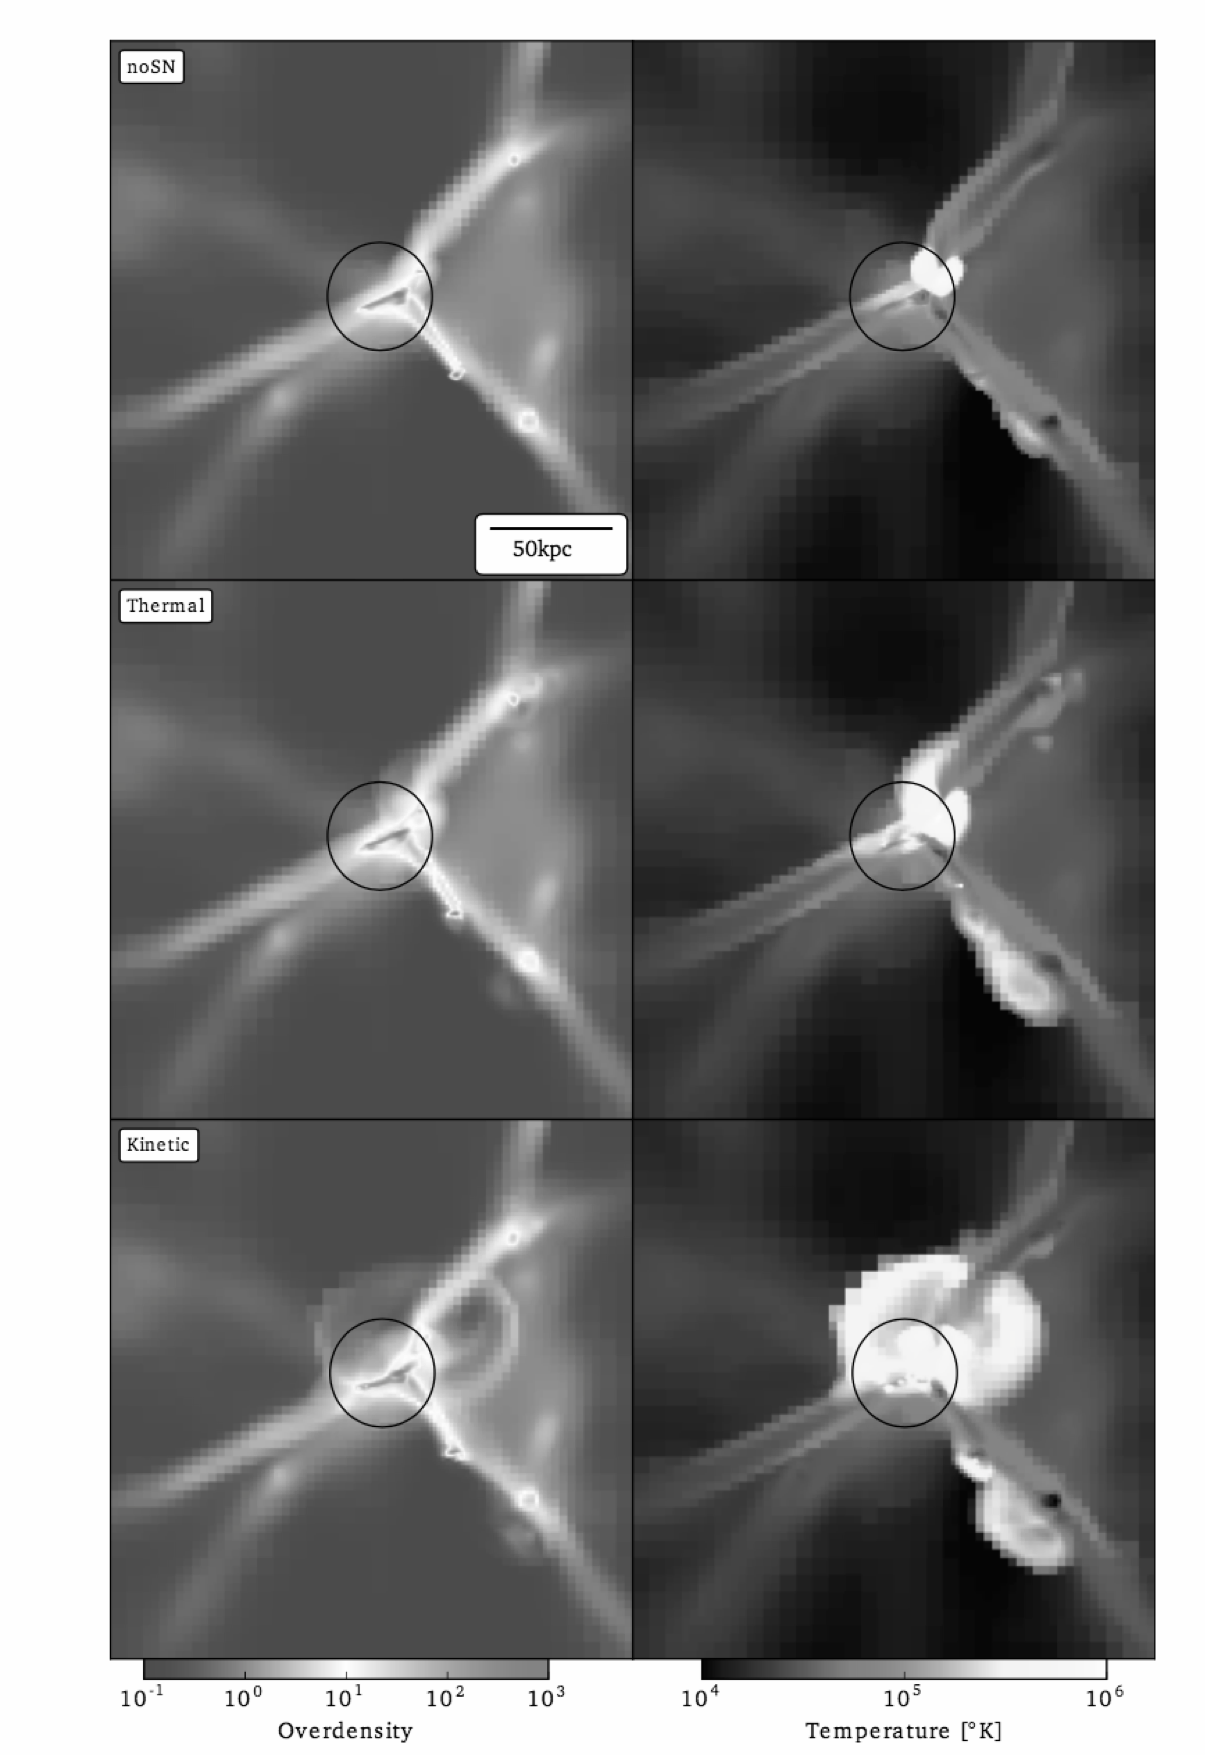
\includegraphics[height=13cm]{figs/SN.png}
	\caption[Exemples d'injection d'énergie par une particule stellaire modélisant l'explosion d'une supernova. ]{Exemples d'injection d'énergie par une particule stellaire modélisant l'explosion d'une supernova. La colonne de gauche montre la densité de gaz autour d'une galaxies pesant $1/10$ème de la masse de la Voie Lactée. La colonne de droite montre la température du gaz. La ligne supérieure montre une simulation sans explosion tandis que les 2 lignes inférieures montrent 2 modèles d'explosion. On note la montée en température du gaz lors de la présence d'explosion ainsi que la création de fronts produits par le gaz expulsé.}
	\label{f:SN}
\end{figure}

\newthought{Les trous noirs supermassifs}\index{trou noir!supermassif} ont aussi un rôle à jouer dans ces modèles à base de simulation. Ils sont en effet les moteurs des \textit{noyaux actifs de galaxies}\index{noyau actif de galaxie}, les AGNs \sidenote{pour \textit{active galactic nuclei}}, qui renvoient dans les galaxies plus massives et leur proche environnement une partie de l'énergie acquise par l'accrétion de matière par le trou noir central. Le taux d'accrétion d'un trou noir de masse $M_\bullet$ est souvent approximée par la formule d'accrétion de Bondi\index{accrétion de Bondi}
\begin{equation}
M_\mathrm{Bondi}\sim \pi \rho v R_s^2.
\end{equation}
Cette formule est une approximation simple du taux d'accrétion autour d'un trou noir se déplaçant à une vitesse $v$ dans un milieu de densité $\rho$ : l'accrétion se fait au travers d'une surface de rayon $R_s=2GM_\bullet/c_s^2$ \sidenote{c'est tout simplement la distance où la vitesse de libération est égale à celle du son}, qui est la distance où la vitesse du son $c_s$ du milieu environnant n'est pas suffisante pour s'opposer à l'attraction. Des particules 'trous noirs' sont ainsi parfois ajoutées dans les simulations cosmologiques et dont la masse va grandir sous l'effet de l'accrétion de matériau pour atteindre parfois des masses de l'ordre du million de masses solaires. Une partie de l'énergie ainsi accumulée va être réinjectée dans le gaz environnant, produisant un effet similaire à la rétroaction des supernovæ créées par les étoiles :
\begin{equation}
E_{\mathrm{TN}}=\epsilon M_\mathrm{Bondi} c^2.
\end{equation}
Contrairement aux étoiles, cette accrétion, et donc cette injection d'énergie, dépend des conditions locales d'accrétion. Ce type de rétroaction est nécessaire pour expliquer par exemple l'abondance des galaxies brillantes, qui est plutôt plus faible que celle attendue par une simple extrapolation du nombre de halos de matière noire\index{halo de matière noire}\sidenote{voir le chapitre dédié à la matière noire} très massifs : l'énergie produite par les AGNs, par effet thermique ou mécanique, réduit l'efficacité de formation stellaire dans ces objets.

\newthought{Tous ces modèles sous-grilles} sont susceptibles de multiples variations dans toutes les étapes, traduisant notre manque de connaissance actuel sur les processus à l'œuvre autour de la formation stellaire ou bien la vue nécessairement grossière de phénomènes fins vus depuis les échelles cosmologiques. Par conséquent les simulations, qui visent à reproduire l'Univers et les galaxies observées, disposent de multiples leviers sur lesquels agir et qui constituent autant de paramètres libres. Par ailleurs, on sait que d'autres physiques sous-estimées ou non modélisées ont peut-être leur rôle à jouer et de fait tout accord entre simulations et observations peut être critiqué\sidenote{comme étant dépendant de l'expérience réalisée ou accidentel par exemple} et tout désaccord peut être minimisé en invoquant une physique mal ou non résolue. La section dédiée à la matière noire survole les quelques problèmes rencontrés par les prédictions numériques : ces problèmes sont la conséquence du caractère beaucoup plus complexe, plus non-linéaire et multiforme des physiques en jeu lorsque l'on quitte le domaine de la cosmologie à proprement dit pour aborder celui de la formation des galaxies. Il n'en reste pas moins que les simulations sont les seuls outils de modélisation nous permettant d'étudier ces processus dans leur plus grande complexité.

%%%!TEX root = /Users/domaubert/Documents/Lectures/cosmologie/cosmo_main.tex
\chapter{Entropie et Univers}
\newthought{La notion d'entropie est profondément liée}\index{entropie} à la cosmologie. En thermodynamique classique, l'entropie est la quantité centrale liée au \textit{second principe}\index{second principe de la thermodynamique} qui stipule que toute transformation d'un système physique s'accompagne d'une création d'entropie $S$\sidenote{notée ainsi en hommage à Sadi Carnot}:
\begin{equation}
\Delta S \ge 0.
\end{equation}
Au mieux, l'entropie reste constante dans le cas d'une transformation dite réversible, mais dans tous les cas elle ne peut diminuer : si cela est malgré tout constaté, cela signifie qu'il existe un autre système, en contact avec celui étudié, qui voit son entropie augmenter d'au moins autant que cette diminution\sidenote{avec $\Delta S_1<0$ et $\Delta S_1 +\Delta S_2>0$}. 

L'une des découvertes fondamentales de la cosmologie est l'affirmation que notre Univers évolue et possède donc une histoire. Conformément à sa définition, cela implique que l'entropie de l'Univers fut plus basse dans le passé qu'elle n'est aujourd'hui. Par ailleurs, l'Univers possède clairement une capacité d'évolution future et son entropie est donc amenée à augmenter. Nous sommes donc aujourd'hui dans un niveau d'entropie intermédiaire, ni à son niveau le plus bas ni à son niveau le plus élevé et cela pose donc naturellement question.

\section{Configurations et probabilités}
\newthought{L'entropie est une mesure} du nombre d'états microscopiques\index{etats@états microscopique} correspondant à un état macroscopique donné. Dans l'ensemble micro-canonique\index{micro-canonique}, décrivant des systèmes isolés à énergie constante, cette brève définition est rigoureusement exacte. L'entropie micro-canonique $S$ est donnée par:
\begin{equation}
S=k_B\log \Omega
\end{equation}
où $\Omega$ désigne le nombre de configurations correspondant à un état macroscopique donné. Le second principe de la thermodynamique\index{second principe} stipule que tout système isolé tend à voir son entropie augmenter avec le temps, au pire elle stagnera si le système atteint un état d'équilibre. Par extension, la flèche du temps\index{flèche du temps} est régie par le sens d'évolution de l'entropie : si 2 possibilités s'offrent à un système, l'une avec une augmentation de l'entropie, l'autre avec une diminution de celle-ci, c'est la première qui sera privilégiée.

Cette croissance imposée à l'entropie peut paraître ad hoc, mais émerge naturellement quand on considère l'entropie micro-canonique. Prenons par exemple un système composé de 4 particules avec 2 éléments gris et 2 éléments rouges (cf. Figure \ref{f:micro}) : ce système peut être \textit{ordonné}\sidenote{ordonné désigne dans notre un exemple un état où les couleurs sont séparées}, un état macroscopique atteint par 2 configurations différentes, ou bien \textit{désordonné}, un autre état macroscopique atteint lui par 4 configurations différentes. Dans l'ensemble micro-canonique, chacune de ces 6 configurations est équiprobable et étant dans une certaine configuration de départ, notre système peut passer dans n'importe quelle autre avec une égale probabilité. Par contre, ce raisonnement ne tient pas lorsqu'on considère les états macroscopiques.
En particulier, si le système est dans un état ordonné, il a dans ce cas 2 fois plus de chances d'évoluer vers un état désordonné que de rester ordonné.  À l'inverse, s’ il se trouve dans un état désordonné, il a deux fois plus de chances de rester désordonné.
\begin{figure}[htbp]
	\centering
		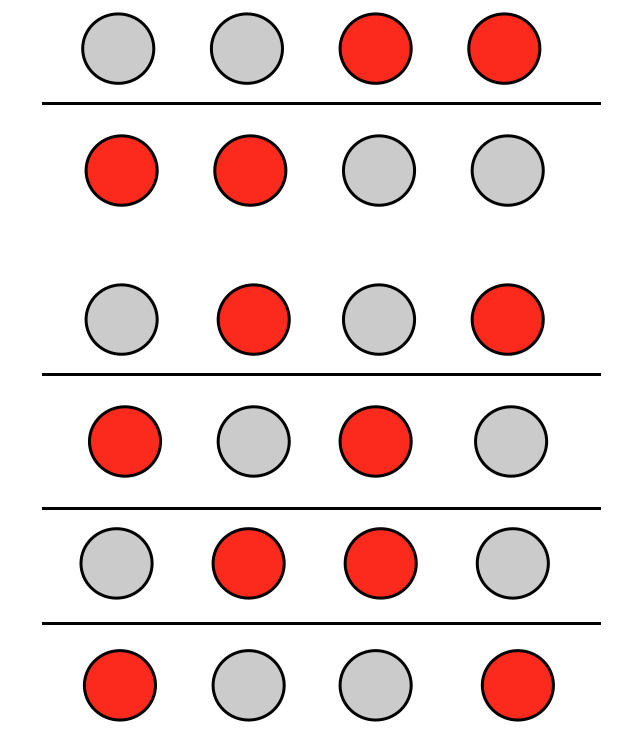
\includegraphics[height=7cm]{figs/micro.png}
	\caption[micro-états disponibles dans un système simple comprenant 2 paires de boules de couleurs identiques]{Tous les micro-états disponibles dans un système simple comprenant 2 paires de boules de couleurs identiques. On note que le macro-état «couleurs séparées» est moins probable que le macro-état «couleurs mélangées».}
	\label{f:micro}
\end{figure}

\newthought{Il n'y a pas de magie noire} : le système évolue vers l'état qui a le plus de chance d'être réalisé. Dans notre cas, l'état mélangé est plus probable que l'état rangé. À l'inverse, l'état rangé est mieux \textit{connu} que l'état mélangé : si le système est dans l'état rangé et que l'on s'interroge sur la «vraie» configuration sous-jacente, on ne peut guère se tromper, car il n'en existe que 2. À l'inverse si le système est dans l'état mélangé, la probabilité de deviner la configuration exacte sous-jacente est 2 fois plus faible : globalement, nous avons une meilleure connaissance de la configuration\index{entropie!configuration} exacte du système s’ il est dans un état de faible entropie. C'est pour cette raison que l'entropie est également une mesure du niveau d'information\index{entropie!information} ou de méconnaissance que nous avons du système : un système avec une entropie élevée est moins bien connu qu'un système à basse entropie et cette connaissance à tendance à se dégrader avec le temps. C'est la contrepartie d'une évolution qui va naturellement vers les états à grand nombre de configurations.

Ces constatations restent applicables pour des systèmes plus complexes ou plus réalistes. Par exemple, le nombre de configurations correspondant à un verre brisé excède de très loin celui correspondant à un verre intact : ce dernier nécessite un arrangement précis des atomes et tout départ léger à cet arrangement conduit à le casser. Par conséquent, l'évolution naturelle d'un verre est d'évoluer vers un état cassé, de plus grande entropie. De même si l'on veut recoller un verre (et donc baisser son entropie), cela est quasi impossible si celui-ci est isolé : il faudrait que spontanément les atomes trouvent l'unique configuration qui corresponde au verre intact parmi toutes celles qui sont associées à un verre brisé. Reconstituer le verre nécessite d'ouvrir le système afin que la baisse d'entropie du verre soit compensée par une augmentation plus globale de l'entropie \sidenote{Par exemple, pour recoller un verre il faut qu'un individu s'attelle à cette tâche. La réflexion de cet individu va nécessairement produire de la chaleur, chaleur qui va globalement augmenter l'entropie}. 

\newthought{La température et l'entropie}\index{température!entropie} sont souvent associées et à nouveau on retrouve dans cette association la notion d'ordre et de désordre, d'information et de méconnaissance. Pour un gaz parfait confiné dans une enceinte, la température est liée à la dispersion de vitesses des particules le composant : on peut montrer que celle-ci est de l'ordre de
\begin{equation}
\sigma \sim \sqrt{k_B T}
\end{equation}
et la distribution de vitesse\index{vitesse!distribution} des particules suit une loi normale\sidenote{type distribution de Maxwell-Boltzmann} d'écart-type donné par cette dispersion (voir Fig. \ref{f:disp}). Si le gaz possède une température élevée, la dispersion de vitesse est importante et par conséquent le spectre des valeurs de vitesses atteignables par une particule est très étendu. À l'inverse, un gaz froid implique une gamme de vitesses accessibles beaucoup plus contrainte.
\begin{figure}[htbp]
	\centering
		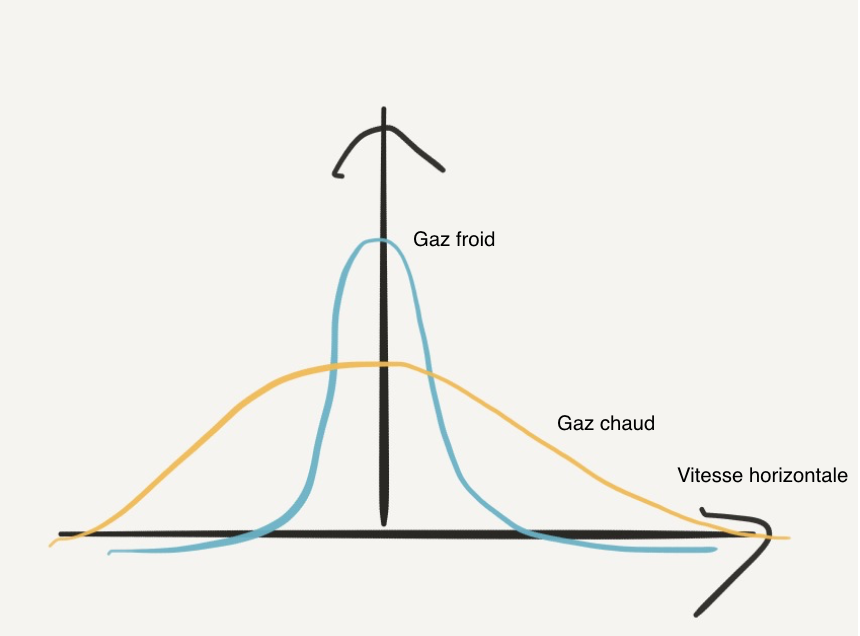
\includegraphics[height=7cm]{figs/dispersion.png}
	\caption[Le lien entre la dispersion de vitesse et la température du gaz. ]{Le lien entre la dispersion de vitesse et la température du gaz. En général, la distribution des vitesses suit une courbe gaussienne, centrée en zéro (la particule n'a pas choisi si elle va à gauche ou à droite) avec des ailes décroissantes. La température est une mesure de la largeur de la distribution: une grande température est la marque de particules à très grande vitesse.}
	\label{f:disp}
\end{figure}
Si l’on considère que ces gaz chauds et froids sont dans la même cuve (donc dans un volume donné), la portion d'espace des vitesses accessible au gaz chaud est plus grande que celle accessible au froid : le nombre d'états correspondant à un gaz chaud est plus important que celui du gaz froid et possède donc une plus grande entropie. Prenant le point de vue inverse, il est plus difficile de prédire la vitesse d'une particule du gaz chaud que pour celle d'un gaz froid. 

Par ailleurs, on dispose d'un certain niveau d'information sur ce mélange : si l’on prend au hasard une particule et que l'on mesure sa vitesse comme étant élevée, on peut sans trop se tromper l'associer au gaz chaud et à l'inverse si sa vitesse est faible, il y a de plus grandes chances qu'elle appartienne au gaz froid. Par conséquent, l'évolution naturelle du système est vers une plus grande méconnaissance, vers la thermalisation\index{thermalisation} des deux gaz vers une même température, intermédiaire entre les 2 températures initiales où le mélange devient tiède. Dans ce cas-là, il y a une perte d'information : la mesure de la vitesse ne permet plus de distinguer les 2 gaz originaux. C'est aussi pour cela que les 2 gaz n'évoluent pas vers une plus grande différence de température, le froid devenant encore plus froid et le chaud encore plus chaud : cela augmenterait notre capacité à distinguer les 2 gaz en tirant les particules au hasard, en contradiction avec la dégradation de l'information posée par le second principe.

\section{Entropie et perception du temps}

\newthought{L'entropie augmente} irrémédiablement lorsqu'un système évolue de manière isolée, toutefois cette augmentation peut ralentir voir s'arrêter. Dans ce dernier cas, le système a atteint un état stationnaire ou d'équilibre\index{etat@état d'équilibre} : cet état macroscopique est le plus probable parmi tous les possibles et possède donc la plus grande chance d'être sélectionné parmi tous ceux accessibles. Un exemple est donné dans la figure \ref{f:equi}. La configuration initiale correspond à un gaz confiné à un sous-volume d'une cuve plus grande : l'évolution naturelle du système va amener le gaz à s'étendre et occuper la cuve dans sa totalité. En supposant que la température du gaz n'évolue pas (et donc que le spectre des vitesses atteignables par les particules reste inchangé), la configuration «cuve remplie» fournit davantage de configurations possibles que lorsque le gaz est confiné dans une sous-partie : dit simplement le nombre de positions accessibles est plus important lorsque le gaz est étendu. L'entropie de la configuration finale est plus importante que celle de départ. 
\begin{figure}[htbp]
	\centering
		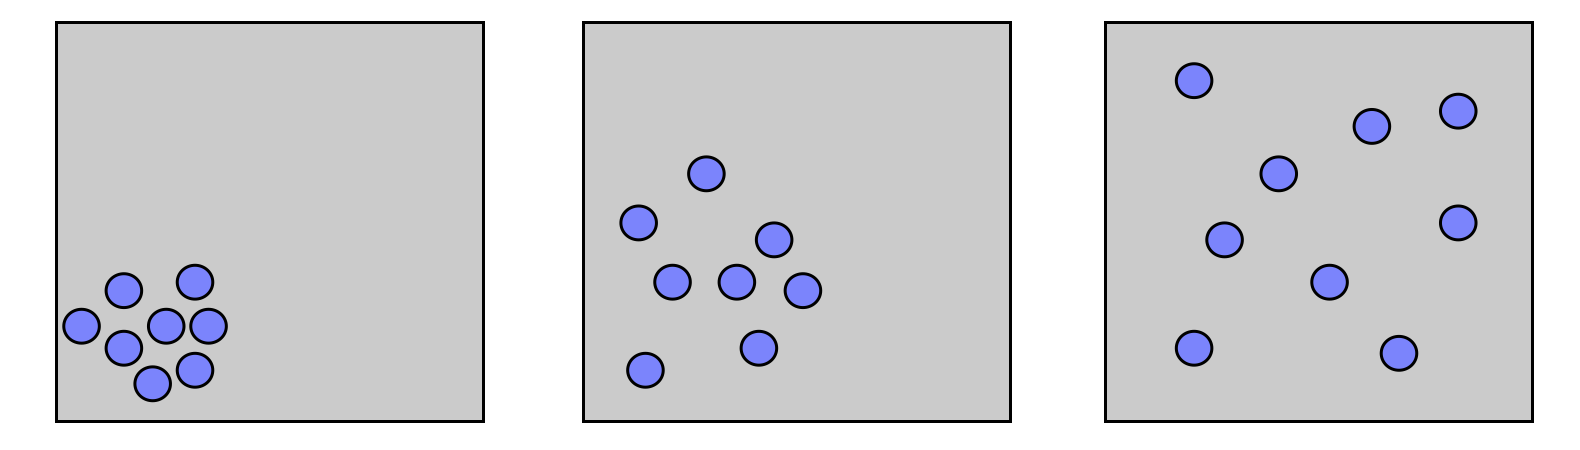
\includegraphics[height=5cm]{figs/equiconfig.png}
		%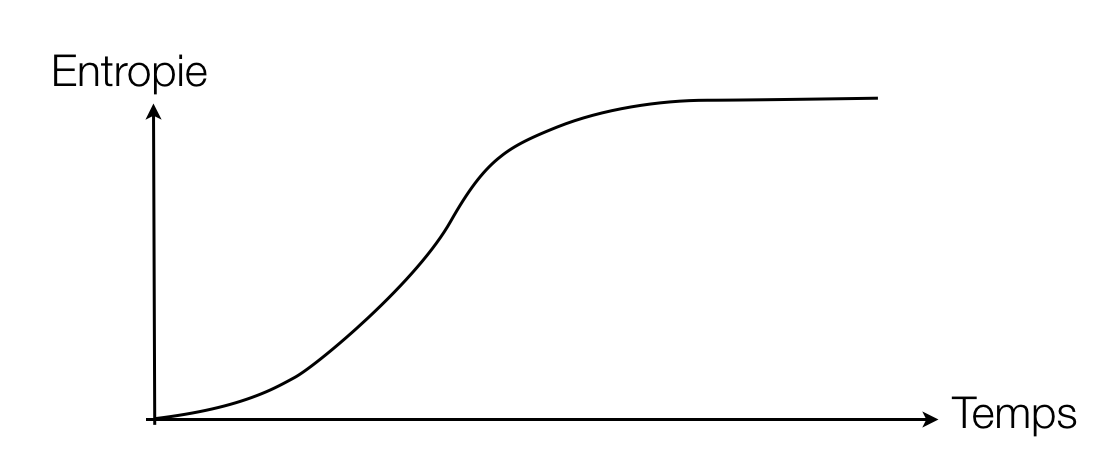
\includegraphics[height=5cm]{figs/equientro.png}
\caption[Remplissage d'une cuve par un gaz]{Le gaz initialement confiné en bas à gauche remplit peu à peu la cuve. La dernière situation a une entropie plus importante que la première, car le nombre de positions accessibles aux particules est plus important. Par contre arrivée à ce stade, l'entropie ne peut plus augmenter de façon significative, on a donc un maximum d'entropie.}
	\label{f:equi}
\end{figure}

Une fois la cuve remplie, le système ne peut cependant plus évoluer et cela correspond à une maximisation des configurations atteignables: le système a atteint un maximum d'entropie\index{entropie!maximum}. Une représentation schématique de l'évolution temporelle de l'entropie est donnée en figure \ref{f:equitemps} : au-delà d'une durée caractéristique \sidenote{intuitivement cette durée $t^*$est liée à la taille de la cuve $L$ et à la vitesse caractéristique $\sigma \sim\sqrt{k_B T}$.  Avec $t^*\sim L/\sqrt{T}$, on constate que l'équilibre est d'autant plus rapidement atteint que la température est élevée.}, $S(t)$ atteint un plateau, autour duquel la valeur peut éventuellement fluctuer, mais jamais redescendre. À ce stade, on constate que le temps est une mauvaise mesure de l'évolution du système: le temps change sans que le système évolue. À l'inverse, l'entropie donne une meilleure représentation de la réalité physique du gaz : l'entropie stagne de la même manière que le système n'évolue plus. Un observateur regardant ce système qui n'évolue plus pourra légitimement dire que le temps a gelé ou bien que le temps est long, car plus rien ne se passe. Par rapport à ce vécu empirique, il apparaît clairement que l'entropie joue un meilleur rôle de représentation de l'évolution du monde : elle augmente lorsque les choses changent, elle stagne lorsque le monde se fige. 
\begin{figure}[htbp]
	\centering
		%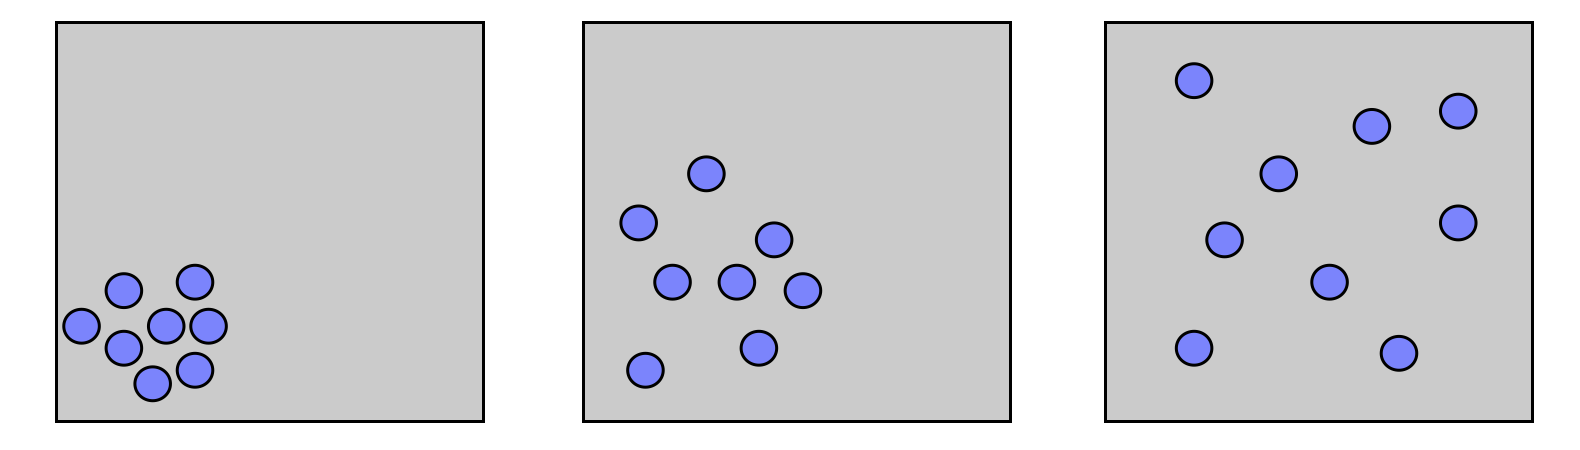
\includegraphics[height=5cm]{figs/equiconfig.png}
		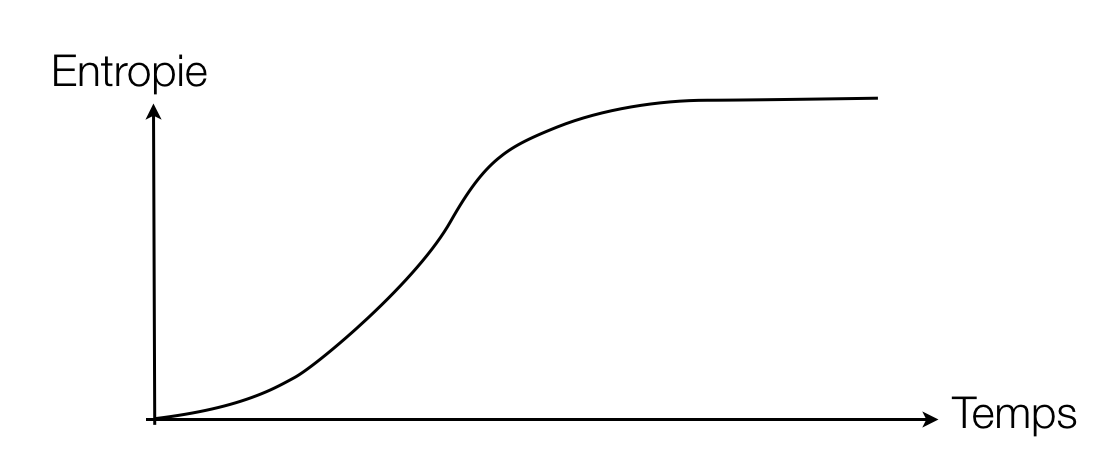
\includegraphics[height=5cm]{figs/equientro.png}
	\caption[Évolution vers un maximum d'entropie]{Un système peut accéder à un maximum d'entropie, auquel cas il n'évolue plus. Le temps est long, car l'entropie est quasi constante. À l'inverse, la phase où l'entropie varie rapidement traduit un système en évolution rapide, durant laquelle le temps s'écoule rapidement.}
	\label{f:equitemps}
\end{figure}

\newthought{Le temps possède une double nature}: c'est d'une part une coordonnée, qui nous permet de nous repérer dans l'espace-temps et une mesure de «distance» qui permet de quantifier le parcours ou le voyage réalisé par un système au cours du temps. Ces deux concepts ne sont pas nécessairement interchangeables et il s'avère que l'on peut se déplacer sans voyager. Par exemple, le voyageur peut arguer du fait qu'un alpiniste ne voyage pas et que son déplacement vertical, tout important qu'il soit sur les plus hauts sommets himalayens par exemple, ne lui permet pas de voir du monde : déplacement et voyage ne vont pas forcément de pair. Le temps et l'entropie\index{temps!entropie} ont le même type de relation : dans une vision entropique le temps c'est du changement et dans une certaine mesure c'est une définition qui est proche de notre vécu empirique. Lorsqu'il ne se passe rien, le temps s'écoule pas ou peu\sidenote{on dit aussi que l'\textit{on trouve le temps long}}. Dans ce régime le temps du chronomètre $t$, celui qui s'écoule inexorablement, est une piètre mesure de la réalité vécue et dans certaines circonstances on aimerait que le temps passe plus vite : dans ces circonstances, c'est réellement $S$ qui est invoqué, et non pas $t$. À l'inverse lorsque les systèmes évoluent rapidement, le temps s'écoule rapidement \sidenote{on dit aussi que l'on trouve que \textit{le temps passe vite}}. Parfois, on aimerait plus de temps ou bien l'on explique que le temps passe trop vite : à nouveau, ce n'est pas le temps $t$ du chronomètre qui est évoqué ici, mais bien l'entropie $S$ dont on  aimerait qu'elle évolue plus lentement.

\section{Entropie et Complexité}
\newthought{On confond souvent entropie et complexité}\index{entropie!complexité}. L'entropie est une mesure du nombre de configurations correspondant à un état macroscopique donné tandis que la complexité est une mesure du nombre d'informations\index{information} qu'il faut pour décrire l'état d'un système. La figure \ref{f:melange} illustre la différence entre ces 2 concepts: on y voit le mélange progressif de 2 gaz de couleurs différentes pour aboutir in fine à un ensemble de couleur homogène. Comme vu précédemment, cette évolution implique nécessairement une augmentation de l'entropie : la situation initiale confine chacun des gaz dans un sous-volume et chaque particule dispose d'un ensemble de configurations spatiales limité. Par ailleurs, l'observateur a une bonne connaissance du système: une particule d'une couleur donnée est assignée à un côté donné. Lorsque le mélange procède, la connaissance de l'état du système se dégrade peu à peu : chaque particule a désormais accès à une plus grande portion du volume et dans l'état final, les 2 fluides disposent de tout le volume pour s'étendre et donc d'un grand nombre de configurations. Par ailleurs, on constate à nouveau une dégradation de l'information puisqu'il est impossible de lier couleur et position.
\begin{figure}[htbp]
	\centering
		%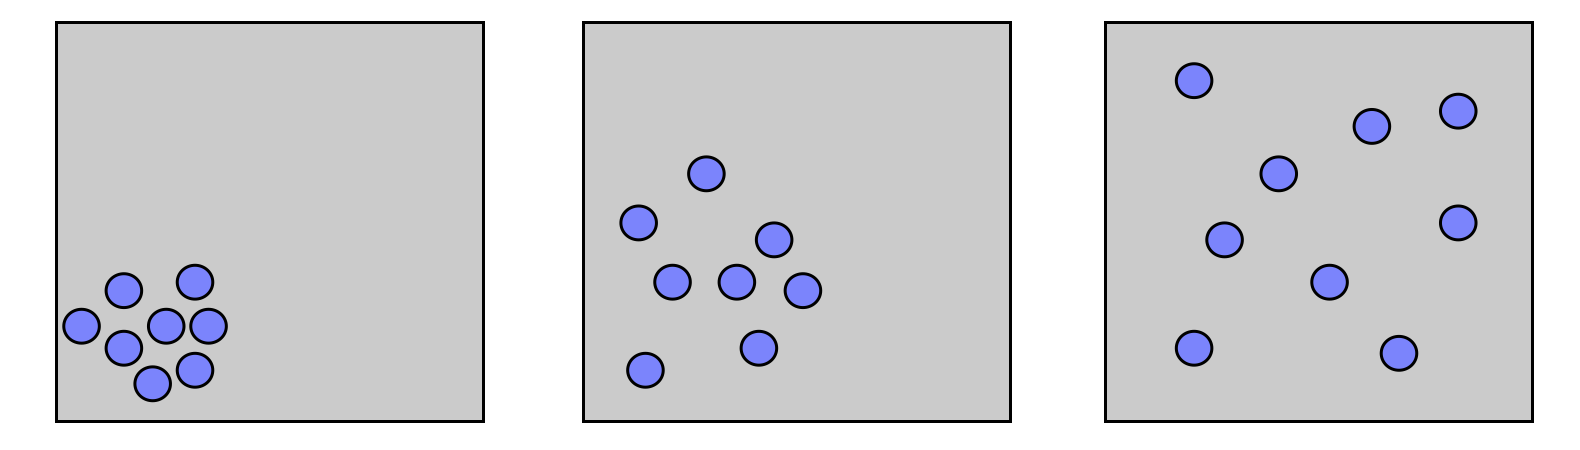
\includegraphics[height=5cm]{figs/equiconfig.png}
		
\includegraphics[height=5cm]{figs/melange.png}
		\caption[Entropie \& Complexité]{Représentation schématique du mélange de 2 gaz. L'entropie va augmenter de gauche à droite tandis que la complexité va passer par un maximum, correspondant à l'état intermédiaire. La présence d'une interface de mélange rend la complexité globale de cette étape très importante. La dernière situation est simple (peu complexe à décrire), mais par contre son entropie est maximale.}
	\label{f:melange}
\end{figure}

La complexité évolue différemment et n'évolue généralement pas de manière monotone. Dans l'exemple précédent, les états initiaux et finaux sont globalement «simples» : l'état macroscopique initial est simple à décrire puisque la position permet de définir la couleur des particules tandis que l'état final l'est encore plus du fait de son homogénéité. L'état intermédiaire en revanche est bien plus difficile à décrire à cause de la zone de mélange : cette zone requiert que l'on établisse un certain nombre de paramètres pour pouvoir être reproduite. Pour cet exemple, la complexité passe par un maximum avant de décroître: l'augmentation de l'entropie nécessite de passer par un pic de complexité. Ce passage par une complexité maximum est souvent la route la plus efficace pour une augmentation de l'entropie. Par exemple, la transformation d'une matière première en chaleur passe souvent par l'intermédiaire d'une «machine» complexe, comme un animal pour de la nourriture ou un moteur pour du carburant.

{Désorganisation et complexité} sont 2 choses différentes : un système peut être dans un état très désorganisé ou peu contraint sans que sa complexité soit grande. C'est le cas de l'état final de l'exemple de la figure \ref{f:melange} : il est simple à décrire, mais pour autant un observateur sait très peu de choses dessus. Sa complexité est faible, mais son entropie est élevée. 

\section{Entropie et formation des grandes structures}
\newthought{Les liens entre cosmologie et entropie} sont nombreux et posent parfois problème. Le plus fameux d'entre eux est l'impression que l'Univers s'organise au cours du temps : durant les premiers instants, le cosmos est par exemple peu structuré et la marche du temps s'accompagne de la mise en place d'objets de plus en plus complexes tels que les étoiles\index{etoiles@étoiles}, les galaxies\index{galaxies} et les amas. Le mécanisme d'instabilité gravitationnelle\sidenote{étudiée en détail dans la section dédiée} donne ainsi l'apparence d'une organisation croissante des objets en contradiction apparente avec le second principe de la thermodynamique. 

Cette contradiction n'est bien sûr qu'apparente et peut être levée de plusieurs façons. Par exemple, on peut aisément invoquer le fait que le processus qui va transformer un nuage de gaz en galaxie n'est pas gratuit. Comme vu précédemment, une galaxie ne peut se mettre en place que si elle parvient à atteindre des densités très élevées \sidenote{typiquement plusieurs milliers de fois la densité moyenne globale}. Or l'énergie interne du gaz (liée à sa pression) s'oppose à ce que de telles densités soient atteintes et cela n'est possible qu'en évacuant cette énergie hors du gaz : dans l'Univers cette évacuation opère via des processus atomiques ou moléculaires qui convertissent l'énergie cinétique microscopique en rayonnement. Ce rayonnement\index{entropie!rayonnement} emporte cette énergie et permet d'atteindre les densités à même de mettre en place des galaxies ou de la formation stellaire en leur sein. Ce processus est producteur d'entropie : des particules (atomes/molécules) en génèrent d'autres, les photons\index{photons}, et parfois en grand nombre. Cette évacuation d'énergie\sidenote{voir le chapitre dédié à la formation des petites structures}, que l'on désigne également par le terme de \textit{refroidissement}\index{refroidissement}, fait grandir le nombre de configurations accessibles par le système par simple production de particules : en augmentant leur nombre, le système augmente le nombre de degrés de liberté et donc son entropie. Par ailleurs, les photons occupent naturellement un grand volume, augmentant d'autant le nombre de configurations possibles pour un état macroscopique donné.  Pour s'organiser, un sous-ensemble de particules (les atomes) va désorganiser l'ensemble en produisant un grand nombre de particules supplémentaires (le rayonnement).

Mentionnons toutefois que ce type de mécanisme où l'entropie est générée en évacuant l'énergie vers l'extérieur n'est pas limité à des processus baryoniques. Pour des systèmes stellaires comme les amas globulaires\index{amas globulaire}, où les constituants n'interagissent que via la gravitation, on trouve également des processus similaires comme la \textit{catastrophe gravothermale}\index{catastrophe gravo-thermale}. Cette dernière consiste en l'effondrement d'un cœur associé à l'expansion d'une enveloppe dans un système non collisionnel. Dans ce processus, l'énergie gravitationnelle libérée par l'effondrement interne va profiter aux couches externes et générer de l'entropie. De même lors de la viriélisation d'un halo\index{halo}, l'effondrement sphérique\index{effondrement sphérique} va «thermaliser» et redistribuer les orbites des particules de matière noire : initialement, toutes ces orbites sont radiales (forte information sur la dynamique, faible entropie) et vont évoluer en un comportement beaucoup plus thermique et désordonné (donc difficile à connaître, forte entropie) après la mise à l'équilibre.

En résumé, la complexité croissante des structures apparaît de prime abord comme en contradiction avec le second principe : toutefois, cette complexité s'accompagne dans tous les cas d'une production d'entropie. De plus, cette complexité ne peut devenir arbitrairement grande : les petites étoiles s'arrêtent et refroidissent, l'expansion accélérée\index{expansion!accélération} créée par la constante cosmologique va supprimer les interactions entre galaxies, les planètes vont cesser de produire de la chaleur\sidenote[][]{cette production est régie par la présence d'éléments radioactifs qui finissent par s'épuiser, cf. Venus ou Mars qui ne possèdent plus d'activité interne.}, etc. ~: ces quelques exemples sont autant d'illustrations de la \textit{mort thermique}\index{entropie!mort thermique} qui attend l'Univers. Cette mort thermique désigne cet état futur où l'entropie ne sera plus en mesure de croître indéfiniment, conduisant de fait à un état d'équilibre de l'Univers. Dans cet Univers, il ne se passe plus rien, l'entropie stagne.

\section{Le défi de l'entropie actuelle}

\newthought{L'entropie actuelle de l'Univers est basse}. Par définition, elle fut encore plus basse dans le passé, mais comparée à ce qu'elle pourrait être, l'entropie actuelle de l'Univers se trouve à de très faibles niveaux\index{entropie!initiale}\sidenote{on peut évaluer l'entropie maximale atteignable par l'Univers et mettant tout son contenu dans un trou noir. L'information ne sort pas de l'objet, la méconnaissance et donc l'entropie est maximale. On en est très loin.}. Par conséquent le potentiel d'évolution de l'Univers est grand et se pose naturellement la question \textit{pourquoi l'entropie actuelle est-elle si basse ?} En effet, imaginons que l'Univers que nous connaissons soit le fruit d'un tirage de lois, paramètres physiques, géométries, etc. parmi tous les ensembles disponibles : normalement, un tel tirage doit naturellement tomber sur les états macroscopiques les plus représentés, les plus probables, donc ceux avec l'entropie la plus forte possible. Dit autrement l'Univers aurait eu toutes les raisons d'avoir une capacité d'évolution faible, avec une entropie élevée, s’ il avait été choisi par hasard : c’est la définition même de la \textit{perfection}\index{perfection}, à savoir un système \textit{qui n'a pas besoin de changer}. Or ce n'est pas le cas, notre Univers n'est pas parfait.

Ce genre de questionnement amène généralement 2 types de réponses~: l'entropie est basse du fait d'un mécanisme ou du fait de conditions initiales. Si c'est le fait de conditions initiales, la question est close et le potentiel d'évolution de notre Univers fait partie de ses propriétés intrinsèques au même titre par exemple que les paramètres cosmologiques. Bien que possible, cette hypothèse nous intéresse peu et la tentation est grande d'essayer de trouver un mécanisme qui produit naturellement une entropie basse aux premiers instants.

Il existe un mécanisme simple et non exotique qui permet d'expliquer une entropie initiale basse : ce mécanisme repose sur la nature statistique des quantités macroscopiques. Lorsqu'un système évolue, son entropie augmente: cette affirmation doit s'entendre de façon statistique. L'entropie est une quantité qui est définie de façon statistique\index{entropie!fluctuation} via par exemple sa valeur moyenne ou son écart-type : sa valeur moyennée sur une certaine durée va augmenter inexorablement dans un système en évolution tout en fluctuant sur des échelles de temps plus courtes. À un instant donné, un système peut voir son entropie baisser ponctuellement avant de reprendre sa croissance\sidenote{nous l'avons vu dans notre exemple simple à base de boules colorées : il est possible de retourner à une situation où les couleurs sont séparées, même si cela est moins probable que de rester dans une situation désordonnée}. On peut imaginer que l'entropie basse de l'Univers fut générée par ce type de fluctuations\index{fluctuation d'entropie} : l'Univers aurait été dans un état de «pseudo-équilibre» avec une entropie constante sur des temps longs et une fluctuation accidentelle et suffisamment grande aurait octroyé à notre Univers un potentiel d'évolution.
\begin{figure}[htbp]
	\centering
		%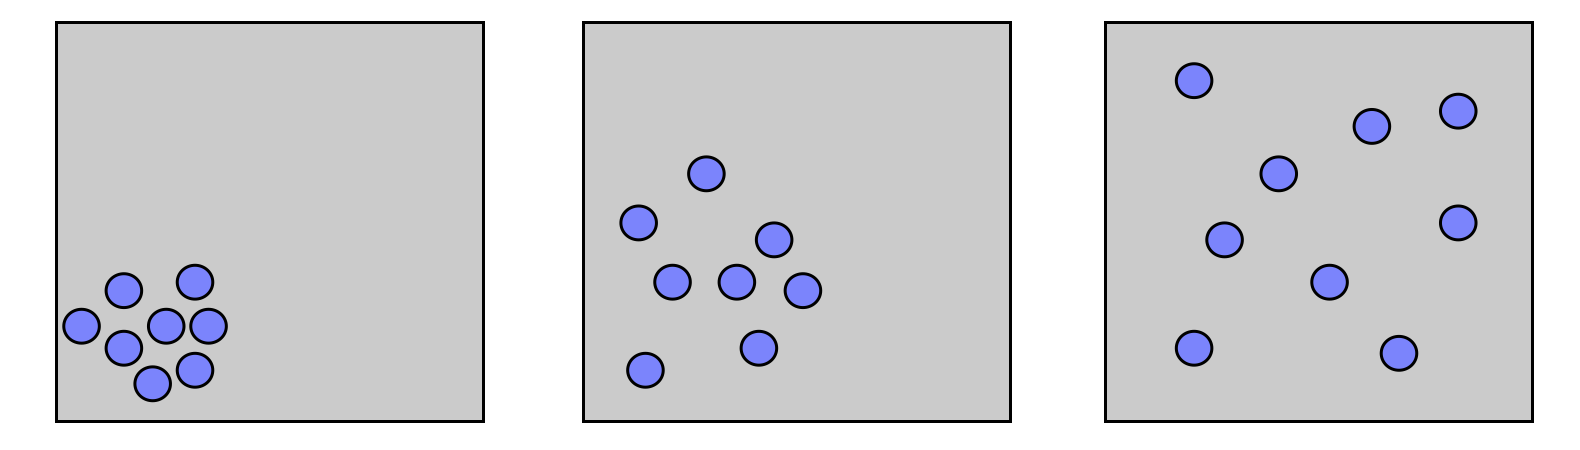
\includegraphics[height=5cm]{figs/equiconfig.png}
		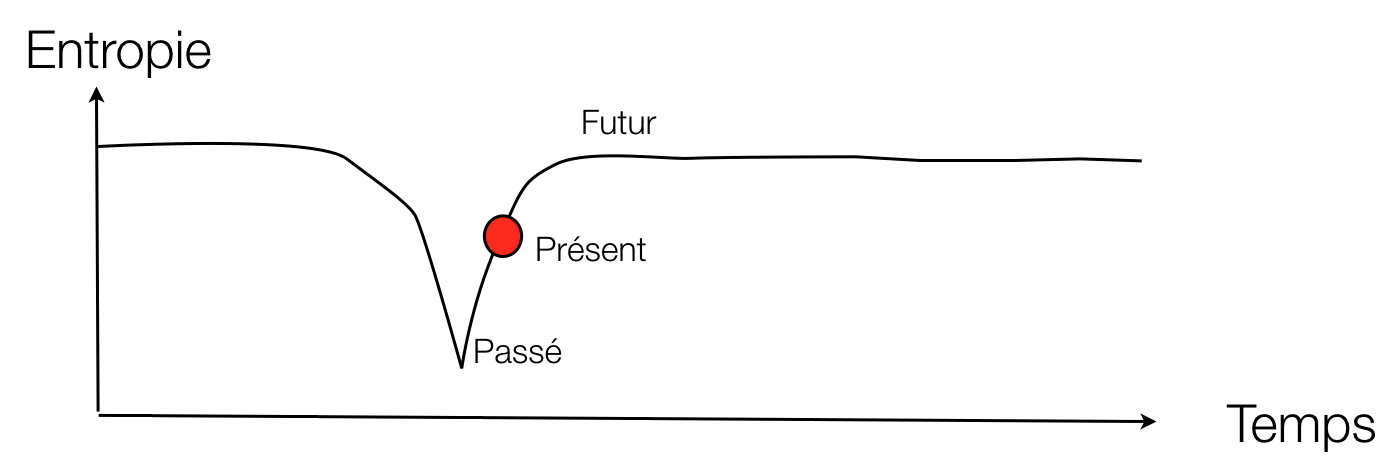
\includegraphics[height=5cm]{figs/fluctuation.png}
	\caption[fluctuation d'entropie]{La possibilité d'une fluctuation d'entropie pour expliquer le démarrage de notre Univers. Passé et futur correspondent aux époques où l'entropie était respectivement basse et haute~: le Big-Bang serait le résultat d'une fluctuation d'entropie sur une situation globale où cette entropie est constante.}
	\label{f:fluctuation}
\end{figure}

Ce scénario a des implications profondes. Dans un premier temps, le point de départ de l'évolution de notre Univers est par définition le Big Bang\index{Big-Bang} : l'instant où cette fluctuation opère correspond donc au début de cette évolution et le Big Bang trouve son origine dans une fluctuation statistique. Par ailleurs, ce scénario suggère que nous sommes dans une phase anormale, précédée et suivie par des états d'équilibres stables qui correspondent aux vrais états naturels de notre Univers : la physique à l'œuvre autour de nous ne serait que la manifestation d'un retour à la normale durant une phase transitoire.

\newthought{Malheureusement, ce scénario souffre d'un paradoxe}. À titre d'exemple, rappelons la définition de l'entropie $S$ dans le cas micro-canonique\index{micro-canonique} :
\begin{equation}
S=k_B\log{\Omega},
\end{equation}
où $\Omega$ désigne le nombre de configurations accessibles pour un état macroscopique donné. Le nombre de configurations correspondant à une valeur d'entropie donnée est :
\begin{equation}
\Omega=e^{S/k_B}.
\end{equation}
Par conséquent, toute fluctuation sur l'entropie est démultipliée exponentiellement et si l’on compare 2 fluctuations d'entropie d'amplitudes différentes, elles conduisent à des nombres de configurations qui sont \textit{exponentiellement} différentes: 2 états microscopiques d'entropies légèrement différentes peuvent correspondre à 2 états de probabilités qui n'ont rien à voir\sidenote{on comprend aisément qu'un macro-état à grand nombre de configurations est plus probable qu'un autre à moins de configurations disponibles}. Une fluctuation d'entropie profonde est donc particulièrement difficile à produire et toute fluctuation d'amplitude intermédiaire est bien plus aisée à mettre en place : l'amplitude de la fluctuation nécessaire à l'évolution constatée autour de nous est de fait quasi impossible à générer. Souvent, on illustre cette difficulté par le \textit{paradoxe des cerveaux de Boltzmann}\index{entropie!cerveaux de Boltzmann} : il est possible que l'Univers tel que nous l'observons soit le fruit d'une sensation ressentie par un cerveau flottant dans le cosmos. Soit un Univers chaotique, rempli de particules~: il est bien plus probable que ces particules s'arrangent brièvement sous la forme de ce cerveau avec ses propres sensations plutôt qu'elles s'organisent par  hasard de façon à créer les conditions qui vont être amenées à créer des étoiles, avec des planètes qui hébergent la vie, vie qui va produire une intelligence en mesure d'étudier le cosmos... Rationnellement, ce cerveau flottant a bien plus de chances refléter la réalité du monde que le second scénario. Bien sûr, cette conclusion est insupportable et de fait probablement fausse, mais elle est inévitable si l'évolution de l'Univers constatée est le fruit d'une fluctuation statistique.

Pour conclure, nous n'avons pas actuellement d'explication simple et satisfaisante concernant la faible valeur initiale de l'entropie cosmique et par extension pour la mise en route de notre Univers en train d'évoluer. Des mécanismes exotiques sont néanmoins proposés, sans validation observationnelle à ce jour~: par exemple, notre Univers est peut-être en communication avec d'autres Univers\sidenote{on parle aussi de \textit{multivers}}, permettant au nôtre d'avoir une entropie faible en augmentant celles des autres cosmos\sidenote{à la manière de réservoirs de gaz en communication}. Ou bien il s'agit simplement d'un tirage favorable des paramètres de notre cosmos, dont une valeur initiale de l'entropie faible~: rappelons que cela fait de notre Univers un monde imparfait, obligé d'évoluer, là où un monde «parfait» pourrait rester statique du fait de sa perfection initiale.  Cet Univers idéal aurait eu des temps caractéristiques d'évolution très longs, durant lesquels rien n'évolue, rien ne se passe ou presque. Et rappelons également qu'une entropie élevée, parfaite, correspond aux configurations les plus nombreuses, les plus probables: nous l'avons échappé belle.
%\chapter{L'inflation et les premiers instants}
\newthought{L'inflation} désigne une phase de l'histoire de l'Univers durant laquelle l'espace aurait rapidement 'enflé', avec des taux d'expansion exponentiels. Cet épisode aurait pris place environ $10^{-34}$ secondes après le Big-Bang et a été suggéré à partir des années 1980 pour expliquer toute une série de défis qui se posent quant à l'état de l'Univers tel que nous l'observons. L'époque inflationnaire reste pour l'instant une hypothèse non vérifiée expérimentalement mais pour laquelle existe tout un faisceau de présomption.

\section{Le problème de l'Horizon de causalité}
\newthought{Le principe cosmologique} repose sur une hypothèse d'homogénéité de l'Univers et cette homogénéité n'est pas remise en question aujourd'hui par les observations. L'une des manifestations les plus spectaculaire de cette homogénéité est la température du fond diffus cosmologique~: comme expliqué dans le chapitre dédié, le fond diffus cosmologique présente une température typique $T\sim 2.7 $K à un très haut niveau de précision (à $10^{-5}$ près) et ceci quelle que soit la direction vers laquelle on regarde \sidenote{on rappelle que c'est cette isotropie qui intrigua Penzias \& Wilson lors de leur découverte du signal}. 

Des anisotropies existent mais elles sont noyées dans l'amplitude du signal du monopole~ : on peut citer l'empreinte des oscillations baryoniques accoustiques, déclenchées par la compétition entre gravité et pression de rayonnement, qui produisent ces grands pics dans le spectre de puissance angulaire du fond diffus. En particulier, les plus grandes échelles angulaires associées à ces ondes accoustiques sont de l'ordre du degré sur le ciel \sidenote{correspondant à une fréquence angulaire $\ell\sim 1000$}. Cette plus grande échelle angulaire correspond à \textit{l'horizon sonore} aux époques de l'émission du fond diffus~: cet horizon est la plus grande distance qui peut être parcourue à la vitesse du son dans les conditions qui y régnaient. Cette vitesse du son est régie par la pression du rayonnement et est de l'ordre de :
\begin{equation}
c_s\sim \frac{c}{\sqrt 3}.
\end{equation}
tandis que l'horizon peut-être approximé par:
\begin{equation}
L_H\sim\frac{c_s}{H}
\end{equation}
On constate donc aisément que l'horizon sonore est proche de l'horizon causal, déterminé lui par la vitesse de la lumière.

Nous avons donc une surface de dernière diffusion qui est isotrope à un très haut niveau de précision \textit{sur toute la sphère céleste} tandis que les échelles de longueurs en contact causal (donc de taille inférieure à l'horizon) sont particulièrement ramassées. Par conséquent, on ne peut trouver de processus physique qui soit en mesure de propager une information sur tout le ciel 380 000 ans après le Big-Bang : cette homogénéité et isotropie ne peut trouver son origine dans un mécanisme physique qui aurait établi ces propriétés sur ces très grandes échelles sans lien causal.

\newthought{Deux possibilités} s'offrent à nouveau : cette isotropie est une condition initiale, particulière mais établie sans raison aucune ou bien cette isotropie est bien le fruit de la propagation d'un signal physique mais sur des échelles plus faibles que celles sur lesquelles l'isotropie est aujourd'hui observée. L'inflation intervient dans ce second scénario : une théorie de l'inflation stipule que l'on ne peut extrapoler l'histoire d'expansion de l'Univers vers le Big-Bang à partir de son contenu actuel et donc de sa dynamique actuelle. Il faut invoquer un épisode où le paramètre d'expansion $a(t)$ connaît une variation soudaine, faisant traverser l'horizon à des échelles en initialement en lien causal. L'idée est simple~: les plus grandes échelles observées sur le ciel étaient sous l'horizon avant l'épisode inflationnaire et sont passées hors-horizon après ce dernier. 

Compte tenu des échelles en jeu\sidenote{on rappelle que l'isotropie est observée sur toute la surface de dernière diffusion, dont le rayon est de l'ordre de plusieurs Gpc}, cette inflation doit impliquer des croissances gigantesques. On verra par la suite que les distances doivent s'accroître typiquement d'un facteur $10^{50}-10^{60}$.

\section{Le problème de la platitude}
\newthought{La géométrie de l'Univers est plane} en moyenne et sur des distances cosmologiques. Dans une telle géométrie, la lumière se propage en ligne droite et la somme des angles d'un triangle fait 180 degrés : comme expliqué dans le chapitre dédié, la taille angulaire des osciallations baryoniques accoustiques mesurée dans le fond diffus à $z\sim1100$ ou dans les grands relevés de galaxies à $z\sim 0$ est hautement compatible avec ce type de géométrie. Un Univers sphérique a tendance à surestimer ces tailles angulaires, un Univers hyperbolique à les sous-estimer et de fait la réalité terrain semble indiquer que le régime à l'oeuvre est exactement entre ces deux régimes.

Tout comme le problème de la causalité, le fait d'avoir une géométrie plane peut soit être le fruit d'un mécanisme qui aurait aplati une géométrie arbitraire ou bien la conséquence d'un choix de conditions initiales particulier. Et à nouveau cette seconde option n'est pas entièrement satisfaisante bien que tout à fait possible. En proposant une augmentation exponentielle des distances, l'inflation fournit naturellement un mécanisme pour gomme toute sorte de courbure~: l'Univers était peut-être doté d'une courbure non-nulle à une époque reculée mais l'Inflation aurait fait tendre toute courbure initiale non nulle vers zéro.

\section{L'origine des fluctuations cosmiques}
\newthought{Les grandes structures de l'Univers} trouvent leur origine dans l'existence de fluctuations dans la distribution spatiale de la densité d'énergie (ou de matière). Ces fluctuations sont observées à de très faibles niveaux dans le fond diffus cosmologique et ce sont ces 'graines' qui servent de point d'ancrage au processus d'instabilité gravitationnelle. Sans ces fluctuations, pas de structures dans l'Univers actuel. 

Comme indiqué précédemment, on attend d'une période inflationnaire qu'elle conduise à un accroissement des échelles de longueurs d'un facteur $\sim 10^{55}$. Si l'on prend une structure de taille 10 Mpc aujourd'hui, un tel facteur conduit à  une taille initiale de l'ordre de $10-{20}$ m, c'est à dire des échelles très largement soumises à des processus quantiques. Par conséquent, on peut imaginer que les structures observées aujourd'hui sont le fruit du passage de fluctuations quantiques à l'échelle macroscopique, par le biais de l'Inflation.
%\chapter{La réionisation}

Chronologiquement parlant, l'époque de Réionisation\index{réionisatoin} désigne la dernière grande transition cosmologique vécue par l'Univers. Ce terme de réionisation désigne la période durant laquelle le gaz d'hydrogène\index{hydrogène} du milieu intergalactique\index{IGM}\sidenote{on parle aussi de la réionisation de l'hélium, plus tardive et que l'on ne mentionnera pas dans ce chapitre} retourne pour l'essentiel à l'état ionisé alors qu'il avait pourtant recombiné lors de l'émission du fond diffus cosmologique. Cette période prend place environ 1 milliards d'années après le Big-Bang, et est le produit de l'apparition des première sources de lumières astrophysiques. Avec la naissance de ces premières sources au sein des précurseurs des galaxies actuelles, la réionisation marque ainsi le début de l'astrophysique non-linéaire, complexe.

\section{Chronologie de la réionisation et propriétés globales}
Environ 380 000 ans après le Big-Bang, la recombinaison laisse place à un Univers rempli d'hydrogène neutre qui va refroidir sous l'effet de l'expansion. Cette période est désignée sous le terme 'd'âges sombres'\index{age@âges sombres} car l'Univers est rempli de gaz n'ayant pas encore réussi à former les premières sources de rayonnement. Ces dernières apparaissent quelques centaines de millions d'années après le Big-Bang : on compte parmi ces sources les première étoiles\index{etoiles@étoiles} et les premiers noyaux actifs de galaxies, dont le moteur central est un trou noir\index{trous noirs} supermassif en accrétion.

\begin{figure}[htbp]
	\centering
		\includegraphics[height=6cm]{figs/frisereion.png}
		\caption[Chronologie de la réionisation]{La chronologie de l'époque de réionisation. Les régions neutre sont claires et les régions ionisées sont sombres. Les zones rouges tracent le gaz chauffé par les explosions de supernovae et le l'effondrement des structures.}
	\label{f:frisereion}
\end{figure}

Ces sources de rayonnement vont produire entre autre du rayonnement ultra-violet\index{fond UV}, capable d'ioniser l'hydrogène cosmique, dont l'énergie de liaison vaut 13.6 eV. Chaque source va alors se voir entourée d'une région ionisée\index{ionisation}, une 'bulle' appelée région HII\index{régions HII}. Sous l'apport continu de photons ionisants par les sources, ces bulles vont grandir et sous l'apparition de plus en plus de sources, ces bulles vont devenir de plus en plus nombreuses. In fine, un réseau de région HII va s'établir puis percoler pour conduire à un Univers totalement ionisé, environ 1 milliard d'années après le Big-Bang. Après cette transition, la fraction résiduelle d'atomes neutres est de l'ordre de $0.01\%$\index{IGM!fraction ionisée}.

En parallèle, cette ionisation va s'accompagner d'un réchauffement du gaz : chaque ionisation va également transmettre de l'énergie à la matière. La température typique du gaz diffus en fin de réionisation est de l'ordre de 10 000 K \index{IGM!température}~: cette température correspond au seuil de refroidissement de l'atome d'hydrogène. Plus chaud, le gaz va évacuer de l'énergie via des processus atomiques, plus froid le gaz est libre de voir sa température augmenter.

\section{Les régions HII}

\begin{figure}[htbp]
	\centering
		\includegraphics[height=10cm]{figs/dX.png}
		\caption[Le réseau de bulles ionisées de la réionisation]{La distribution de gaz ionisé dans un Univers en cours de réionisation d'après un calcul de simulation numérique. Les régions jaunes sont ionisées et chaudes, centrées autour des régions qui forment des étoiles. L'image fait environ 90 Mpc de côté et réprésente un Univers à z=8 environ à mi-réionisation.}
	\label{f:dX}
\end{figure} 

La création de 'bulles' ionisées autour des premières sources est le processus élémentaire à l'origine de la réionisation complète de l'Univers : ces bulles sont appelées régions HII\index{régions HII}\sidenote{HI étant une dénomination de l'hydrogène neutre. Par analogie on parle de HeI, HeII et HeIII pour désigner l'hélium neutre, ionisé une fois et deux fois.} L'étendue de ces régions est régie par la compétition entre 2 effets aux conséquences opposées:
\begin{itemize}
\item d'une part la production de photons ionisants par une source\index{ionisation}. Ces photons ionisant grignotent le gaz neutre et tendent à faire grandir la région HII
\item d'autre part la tendance naturelle des électrons libres à recombiner\index{recombinaison} avec les noyaux pour reconstituer des atomes. Cette recombinaison à l'inverse a tendance à réduire la taille de ces régions ionisées.
\end{itemize}
Une simple équation permet de faire la synthèse de cette compétition \sidenote{$N_H$ désigne la densité numérique d'atomes d'hydrogène neutres (en m$^{-3}$), $N_{H+}$ celle d'atomes ionisés, $N_e$ celle des électrons libres}:
\begin{equation}
\frac{d n_H}{dt}=\alpha n_{H+}n_e -\Gamma n_H.
\end{equation}
Ici $\alpha(T)$ est le taux de recombinaison de l'hydrogène : il dépend de la température\sidenote{un gaz froid a tendance à recombiner plus efficacement} et possède les dimensions d'un volume par unité de temps. Cette quantité, et donc le terme associé dans cette équation différentielle, encode la capacité du gaz ionisé à redevenir spontanément neutre.  A l'inverse $\Gamma$ est le taux de photoionisation et dépend du nombre de photons ionisants produits et présents dans la bulle ionisée.

Plutôt que de raisonner en abondance de protons et d'électrons, il est d'usage d'introduire la fraction d'ionisation $x$:
\begin{equation}
x=\frac{n_{H+}}{n_{H+}+n_H}
\end{equation}
qui renvoie simplement le fraction d'atomes ionisés par rapport au nombre total de noyaux d'hydrogène disponibles (sous forme atomique ou non). Cette fraction ionisée sera une quantité centrale pour décrire la réionisation cosmologique. En négligeant la contribution des éléments autres que l'hydrogène au gaz cosmique\sidenote{on rappelle que son abondance est proche de $95\%$ en nombre} et en utilisant le principe d'équilibre des charges électrique, le terme de recombinaison peut s'écrire:
\begin{equation}
n_\mathrm{rec}=\alpha x^2 n^2
\end{equation}
où $n=n_{H+}+n_H$ désigne la densité totale de protons. Si la région est complètement ionisée, $x=1$ et ce terme devient simplement:
\begin{equation}
n_\mathrm{rec}=\alpha n^2.
\end{equation}
Si on modélise la région HII par une sphère de rayon $R$, le nombre total de recombinaisons par seconde à l'intérieur est donné par:
\begin{equation}
N_\mathrm{rec}=\frac{4}{3}\pi R^3\alpha n^2.
\end{equation}
Si ce nombre de recombinaison est égal au nombre de photons ionisant produits par seconde$ \dot N_\mathrm{ion}$, la région ionisée ne peut s'agrandir et on obtient une sphère, stationnaire, dite de \textit{Strömgren}\index{sphère de Strömgren}, dont le rayon $R_s$ satisfait:
\begin{equation}
\frac{4}{3}\pi R_s^3\alpha n^2=\dot N_\mathrm{ion}.
\end{equation}
Cette région HII, stationnaire, possède donc un rayon donné par :
\begin{equation}
R_s=\left(\frac{3 \dot N_\mathrm{ion}}{4\pi \alpha n^2}\right)^{1/3}.
\end{equation}
Plus la production de photons\index{photons} est importante, plus ce rayon est important et à l'inverse un milieu dense en atome, ou recombinant plus facilement à cause d'une basse température, présentera un rayon stationnaire plus petit.

Le cas non-stationnaire, avec un front en cours de progression, est plus délicate à obtenir. Une approche possible consiste à considérer qu'un observateur lié au front d'ionisation voit d'un côté de ce front un flux de masse neutre et de l'autre un flux de masse ionisée, contraint par le flux de photons ionisant local. Ces 2 flux doivent être égaux \sidenote{$m$ désigne la masse d'un atome d'hydrogène, $v$ la vitesse du front\index{vitesse!front d'ionisation} et $F$ le flux de photons ionisants}:
\begin{equation}
m n v = m F_\mathrm{ion}.
\end{equation}
La vitesse du front satisfait donc:
\begin{equation}
v=\frac{1}{n}\frac{\dot N_\mathrm{ion}(r_f)}{4\pi r_f^2}.
\end{equation}
Le taux de photoionisation disponible au niveau du front est le taux de photoionisation total moins le nombre de recombinaison à l'intérieur du front:
\begin{equation}
\dot N_\mathrm{ion}(r_f)=\dot N_\mathrm{ion}(0)-\frac{4}{3}\pi r_f^3\alpha n^2=\frac{4}{3}\pi \alpha n^2 (R_s^3-r_f^3),
\end{equation}
d'où l'équation différentielle sur la position du front $r_f$ :
\begin{equation}
3r_f^2\frac{d r_f}{dt}=\frac{dr_f^3}{dt}=\alpha n  (R_s^3-r_f^3).
\end{equation}

\begin{figure}[htbp]
	\centering
		\includegraphics[height=10cm]{figs/strom.png}
		\caption[Evolution temporelle de la position d'un front ionisant]{Evolution temporelle du rayon d'une région HII. Les rayons sont exprimés en unités du rayon de Strömgren, correspondant à l'état final stationnaire, tandis que les temps sont exprimés en temps de recombinaison. On constate que les modèles à temps de recombinaison courts, donc efficaces, ont des rayon d'équilibre plus petits et les fronts sont stoppés plus rapidement.}
	\label{f:strom}
\end{figure}

La solution sur la position du front \sidenote{en posant $y=(r_f/R_s)^3$, on peut reconnaître une simple équation différentielle du premier ordre avec second membre constant} est alors donnée par:
\begin{equation}
r_f(t)=R_s(1-e^{-t/t_\mathrm{rec}})^{1/3},
\end{equation}
la position du front converge vers le rayon de la sphère de Strömgren\index{sphère de Strömgren}, sur une durée caractéristique $t_\mathrm{rec}=(\alpha n)^{-1}$, qui n'est autre que le temps de recombinaison\index{temps!recombinaison} caractéristique du gaz. Si le gaz recombine rapidement, la front ionisant stoppe rapidement et le rayon se stabilise. A l'inverse un gaz diffus ou chaud, à faible pouvoir de recombinaison va voir ses fronts aisément se propager. Dans la figure \ref{f:strom}, on constate dans tous les cas que la progression initiale des fronts est toujours rapide puis tend à ralentir lorsque les recombinaisons commencent à faire effet (pour $t\sim t_\mathrm{rec}$). La température typique du gaz intergalactique \index{IGM!température}est de l'ordre de $T=10 000 K$, tandis que les densités d'atomes pour des filaments de gaz intergalactiques sont environ de 1000 atomes/$m^3$. Dans ces conditions, les temps de recombinaison typiques sont de l'ordre de 100 millions d'années.

\section{Elements de transfert radiatif}

Bien sûr le cas de la région HII décrit précédemment est idéalisé : dans le cas cosmologique la densité d'atomes n'est pas homogène, le gaz réagit dynamiquement à la présence du front, la température n'est pas constante et bien sûr l'expansion de l'Univers conduit à une densité qui n'est pas constante au cours du temps. Par ailleurs, les sources de rayonnement ne sont pas stationnaires, elles vivent des histoires compliquées et s'influencent les unes les autres. Pour résoudre le problème dans toute sa complexité, il faut utiliser des simulations cosmologiques capables de modéliser la physique du \textit{transfert} radiatif\index{transfert radiatif}, la physique de l'interaction de la matière avec le rayonnement. 

La base du transfert du rayonnement est la résolution de l'équation du transfert radiatif qui décrit l'évolution de l'intensité du rayonnement $I_\nu({\bf x},{\bf n} ,t)$ \sidenote{$I_\nu$ désigne l'intensité spécifique du rayonnement, $S_\nu$ les sources de rayonnement et $\kappa_\nu$ l'absorption}:
\begin{equation}
\frac{1}{c}\frac{\partial I_\nu}{\partial t}+{\bf n} \frac{\partial I_\nu}{\partial {\bf x}}=S_\nu - \kappa_\nu I_\nu.
\end{equation}
En plus du temps, cette intensité dépend de la position $x$, de la fréquence $\nu$ et de la direction de propagation $\bf n$~: on se trouve donc face à un problème de très grande dimensionnalité (7 dimensions)~: l'équation du transfert est pour l'essentiel une équation de conservation de la fonction de distribution des photons\index{photons!distribution} dans l'espace des phases.

Il existe plusieurs manière de 'simplifier' sa résolution, en réduisant sa dimensionnalité. L'une des plus communes consiste à considérer une source à l'origine seulement\sidenote{on néglige ainsi les sources diffuses, comme celles dues à la recombinaison atomique} et à supposer que la lumière est instantanément absorbée en chaque point. Le long de la direction de propagation, l'équation du transfert se réduit alors à:
\begin{equation}
 \frac{\partial I_\nu}{\partial {\bf x}}=- \kappa_\nu I_\nu.
\end{equation}
Le long du rayon, la solution est alors:
\begin{equation}
I_\nu(x)=I_\nu(x=0)e^{-\int_0^x \kappa_\nu dx}=I_\nu(x=0)e^{-\tau},
\end{equation}
cette solution est une classique exponentielle décroissante, dont la grandeur caractéristique est \textit{l'opacité} $\tau$ mesurée le long du rayon\index{opacité}. Plus cette opacité est importante le long de la direction de propagation, plus le rayonnement est atténué. Si on dispose d'un modèle de distribution des sources dans l'espace, on peut donc tracer des rayons\index{transfert radiatif!lancer de rayons} dans toutes les directions et calculer cette opacité le long de tous ces rayons~: cette donnée permet d'évaluer la quantité de rayonnement partout et donc le taux de photoionisation partout pour modéliser la réionisation.

Une autre approche consiste à prendre les moments\index{transfert radiatif!moments} de l'équation du transfert radiatif, pour évaluer la densité ou le flux de rayonnement\index{flux!rayonnement} par exemple:
\begin{eqnarray}
N_\nu&\sim&\int I_\nu d^3{\bf n}\\
{\bf F}_\nu&\sim&\int {\bf n} I_\nu d^3{\bf n}
\end{eqnarray}
Ces quantités ne dépendent plus que de la position et satisfont leurs propres équations de conservation\sidenote{en négligeant les termes sources}:
\begin{eqnarray}
\frac{1}{c}\frac{\partial N_\nu}{\partial t}+\frac{\partial {\bf F_\nu}}{\partial {\bf x}}&=&-\kappa N_\nu\\
\frac{1}{c}\frac{\partial F_\nu}{\partial t}+\frac{\partial {\bf P_\nu}}{\partial {\bf x}}&=&-\kappa' F_\nu.
\end{eqnarray}
On a donc affaire à un système d'équations dites hyperboliques, similaires aux équations de l'hydrodynamique\sidenote{conservation de la masse et équation d'Euler} et qu'on peut alors résoudre à l'aide des même techniques. Toutefois, cela nécessite de fermer le système d'équation avec une équation d'état du rayonnement liant la pression\index{pression!rayonnement} radiative $\bf P$ avec la densité de rayonnement par exemple~: il existe toute une série de modèles qui fournissent ce type de relation en fonction du problème physique considéré. On peut par exemple se contenter de l'équation de conservation de la densité de rayonnement et imposer que le flux radiatif soit simplement lié au gradient de cette densité:
\begin{equation}
{\bf F_\nu}=-\nabla N_\nu,
\end{equation}
le rayonnement va alors 'couler' des régions brillantes aux régions éteintes. Simple à mettre en place, ce modèle souffre toutefois de l'impossibilité de créer des ombres derrières des absorbants denses par exemple.

\section{Observer la réionisation de l'Univers}
L'époque de réionisation\index{réionisation} s'achève à $z\sim 6$, correspondant à un Univers âgé environ de 1 milliard d'années. Son début est beaucoup plus incertain : la transition démarre avec l'apparition des premières sources, très probablement des étoiles, mais l'instant de leur apparition n'est pas connu. On pense aujourd'hui qu'il faut quelques centaines de millions d'années pour que le gaz puisse acquérir les conditions lui permettant de former ces premières sources, correspondant à des redshift $z\sim 30- 50$. Ces époques sont particulièrement reculées, donc distantes, et sont donc particulièrement difficiles à observer.  On dispose aujourd'hui de 2 grandes observations qui démontrent que la transition a bien eu lieu : la forêt Lyman-$\alpha$ et l'étude du fond diffus cosmologique.

\subsection{Le milieu intergalactique, la Forêt Lyman-Alpha}
La première observation 'canonique' de la Réionisation est l'étude de la forêt Lyman-Alpha\index{forêt Lyman-$\alpha$}. Ce terme désigne les spectres de sources brillantes lointaines (généralement des quasars) qui présentent des systèmes de raies d'absorption denses aux fréquences plus élevées que la raie Lyman-Alpha de l'hydrogène\index{hydrogène}\sidenote{dont la longueur d'onde est 121.6 nm}. Le principe qui conduit à l'apparition de ces raies est simple : ces sources possèdent un spectre continu et une raie Lyman-alpha en émission. Au cours de leur propagation les photons associés vont se décaler vers le rouge : si jamais un photon rencontre un nuage d'hydrogène neutre au sein du milieu intergalactique, ce dernier va générer une raie\index{raie d'absorption} en absorption à 121.6 nm dans son référentiel. Toutefois, comme le spectre de la source lointaine perçu par le nuage est décalé vers le rouge, l'absorption va se faire à une fréquence plus élevée que celle de la raie en émission. Si jamais un second nuage se trouve sur la ligne de visée, une autre absorption va s'ajouter ~: comme le spectre de la source lointaine s'est encore d'avantage rougi\index{rougissement}, cette raie d'absorption supplémentaire se placera dans les parties plus bleues, à plus haute fréquence, que la raie créée par le premier nuage et que celle de la raie en émission. Par extension si de multiples nuages sont présents sur la ligne de visée, chacun d'entre eux va générer une raie en absorption qui prises globalement donne l'apparence d'une 'forêt' de raies.

\begin{figure}[htbp]
	\centering
		\includegraphics[height=12cm]{figs/lya.png}
		\caption[Principe de la forêt Lyman-$\alpha$]{La fôret Lyman-$\alpha$ est un ensemble de raies d'absorptions créées par des nuages neutres absorbants le long de la ligne de visée vers une source lointaine brillante. Chaque nuage perçoit le spectre de la source de façon décalée à cause de l'expansion cosmologique et va donc placer une raie d'absorption à sa propre fréquence correspondant à 121.6 nm dans son référentiel.}
	\label{f:lya}
\end{figure}

La forêt Lyman-Alpha est un outil particulièrement puissant puisqu'elle permet de tracer la distribution spatiale des nuages de gaz neutres le long de la ligne de visée ou leur température. On a donc accès à l'état du milieu intergalactique\index{IGM} sur toute une gamme d'époques. Si par ailleurs on dispose de multiples lignes de visées, il est possible de réaliser de la \textit{tomographie}\index{tomographie}, c'est à dire une reconstruction 3D de la structure du milieu intergalactique, entre ces sources et nous.

Que se passe-t-il si la source émet ses photons dans une époque antérieure à la réionisation ? Au lieu d'avoir une discontinuité de nuages neutres absorbants, l'ensemble du milieu intergalactique\index{IGM} est capable de produire une absorption. L'observateur constate alors une continuité d'absorption aux longueurs d'ondes plus courtes que l'émission Lyman-$\alpha$ et dans les cas les plus extrême, la transmission est proche de zéro : le spectre présente alors un \textit{Gunn-Peterson Through}\index{Gunn-Peterson}\sidenote{on pourra le traduire par 'Tunnel' Gunn-Peterson}, caractérisé par une absence de signal sur une grande gamme de longueurs d'ondes. C'est précisément ce qui est obtenu lorsque l'on observe des spectres de quasars de plus en plus en lointains, de plus en plus enfouis dans l'époque de réionisation~: la disparition graduelle de la forêt indique la mise en place d'un Univers rempli de gaz neutre absorbant aux alentours d'un redshift $z\sim 6$.
\begin{figure}[htbp]
	\centering
		\includegraphics[height=12cm]{figs/fan06.png}
		\caption[Spectres de quasars durant la réionisation]{Un échantillon de spectres de quasars émettant durant l'époque de réionisation. Les quasars du bas émettent après la réionisation dans un Univers ionisé et transparent au rayonnement UV~: on observe du signal aux longueurs d'ondes plus courtes que la raie d'émission Lyman-$\alpha$. Ceux du haut en revanche sont situé avant la réionisation~: leurs spectres sont davantages décalés vers le rouge et surtout on constate pour certains d'entre eux une absence totale de signatures spectrales avant la raie d'émission. C'est la marque d'un Univers rempli de gaz neutre. Figure extraite de Fan et al. 06.}
	\label{f:fan06}
\end{figure}

\subsection{L'opacité Thomson du CMB}
La réionisation\index{réionisation!fond diffus}\index{fond diffus} va produire des électrons libres aux alentours d'un redshift de 6. Or ces électrons vont naturellement avoir tendance à interagir avec les photons du fond diffus cosmologique tandis que ces derniers volent vers un observateur terrestre~: ce processus de diffusion dit Thompson\index{diffusion Thompson} va affecter la structure angulaire du fond diffus cosmologique, particulièrement aux grandes échelles. Cet effet peut-être évalué quantitativement et donc mettre des contraintes sur l'histoire de la réionisation.

\begin{figure}[htbp]
	\centering
		\includegraphics[height=10cm]{figs/ne.png}
		\caption[La densité d'électrons cosmique]{La densité physique d'électrons pour 3 modèles simples de réionisation instantanée et complète. L'opacité Thompson, le taux d'interaction des électrons avec les photons du CMB, est donnée par l'intégrale de cette courbe : plus la réionisation est précoce, plus l'opacité est importante.}
	\label{f:nereion}
\end{figure}

La quantité importante s'appelle l'opacité Thompson\index{opacité!fond diffus} et est calculée de la manière suivante:
\begin{equation}
\tau_\mathrm{th}=\int_{z_\mathrm{rec}}^{z=0} c \sigma_T n_e(z) dt
\end{equation}
et revient de fait à calculer une histoire intégrée de la production d'électrons libre $n_e$ au cours de l'histoire cosmique. En théorie, le calcul de la valeur de l'opacité dépend de l'histoire détaillée de réionisation mais il est facile de comprendre le comportement qualitatif de cette quantité à partir d'un modèle simple. En effet, supposons que la réionisation soit parfaite de telle manière à ce que tous les atomes d'hydrogènes soient ionisés et qu'elle soit instantanée. Dans ce cas la densité comobile d'électrons libres est simplement constante ~: elle est nulle avant la réionisation et vaut \sidenote{on considère que l'hélium est absent}:
\begin{equation}
n_\mathrm{e,com}=\frac{\Omega_b \rho_c}{m_p}
\end{equation}.
La densité \textit{physique} d'électrons, celle nécessaire au calcul de $\tau_\mathrm{th}$, est donc simplement nulle avant la réionisation et après la réionisation vaut (voir Fig \ref{f:nereion}):
\begin{equation}
n_e(z<z_\mathrm{reion})=\frac{\Omega_b \rho_c}{m_p} \frac{1}{(1+z)^3}.
\end{equation}
La valeur de l'opacité vaut donc:
\begin{equation}
\tau_\mathrm{th}=\int_{z_\mathrm{rerion}}^{z=0} c \sigma_T\frac{\Omega_b \rho_c}{m_p} \frac{1}{(1+z)^3}  |\frac{dt}{dz}| dz.
\end{equation}

Plus le redshift de réionisation est élevé (plus la transition est précoce) plus la valeur de $\tau_\mathrm{th}$ est importante. De fait les premières mesures de cette quantité par le satellite WMAP, donnait des valeurs de $\tau_\mathrm{th}\sim 0.17$ correspondant à des redshifts de réionisation proches de $17$. Comparés à ceux obtenus par la technique des spectres de quasars, la tension était particulièrement forte entre les types de sondes de la réionisation. Depuis, les mesures successives, via le satellite WMAP ou Planck\index{Planck!satellite} on ramené cette quantité à des valeurs plus raisonnables, de l'ordre de $\tau_\mathrm{th}\sim 0.068$ ce qui correspond à des redshifts de \textit{mi-réionisation} de l'ordre de 8 : cette valeur est bien plus compatible avec celle mesuré via la forêt Lyman-$\alpha$. Toutefois, et de façon un peu paradoxale, une faible valeur de $\tau_\mathrm{th}$, donc une réionisation plus tardive, a tendance à rendre le CMB moins pertinent pour l'étude de l'époque de réionisation~: en effet, une faible valeur indique un faible couplage entre les électrons de la réionisation et les photons du CMB, et par extension ces photons sont moins sensibles à cette réionisation. Physiquement la raison en est simple~: une réionisation tardive implique une densité physique d'électrons libres plus faibles que celle qui aurait été obtenue pour une réionisation précoce.

\begin{figure}[htbp]
	\centering
		\includegraphics[height=12cm]{figs/tau.png}
		\caption[L'opacité Thomson du CMB]{La distribution des valeurs possibles de $\tau_\mathrm{th}$ d'après les mesures du satellites Planck. Les différentes courbes représentent les différentes estimations en considérant soit les données Planck en température seules (courbes bleues) soit en les couplant à d'autres mesures (par exemple les BAOs dans la distribution des galaxies) pour contraindre davantage cette mesure. La meilleure estimation donne $\tau_\mathrm{th}\sim 0.066 \pm 0.016$ équivalant à un redshift de mi-réionisation proche de 8.8. Figure extraite de Planck XIII.}
	\label{f:tau}
\end{figure}

\subsection{le signal à 21 cm}
 Contrairement aux 2 mesures précédentes, celle-ci n'a pas encore été réalisée dans le cas de la réionisation mais elle est des plus prometteuses. Il s'agit de détecter le signal émis directement par le gaz d'hydrogène neutre, à la longueur d'onde de 21 cm\index{signal à 21 cm}. Ce signal radio correspond à la transition entre les 2 états de spin de l'électron sur le niveau fondamental\sidenote{on parle de transition hyperfine}\index{transition hyperfine}~: clairement l'écart d'énergie entre les 2 configurations doit être très faible, et le rayonnement produit est à très basse énergie. Le signal à 21 cm du gaz neutre peut s'exprimer sous la forme d'une température de brillance:
 \begin{equation}
 \delta T_b \sim x_\mathrm{HI} (1+\delta) (1-\frac{T_\mathrm{CMB}}{T_S})(1+\frac{1}{H}\frac{d v_r}{dr})^{-1}.
 \end{equation}
 Ce signal est extrêmement riche physiquement. Il dépend de l'état d'ionisation de l'hydrogène : un gaz complètement ionisé ($x_\mathrm{HI}=0$) donne un signal nul, comme attendu~: au cours de la réionisation, la mise en place d'un réseau de bulles ionisées doit donc directement se manifester dans ce signal radio. Il dépend aussi directement de la densité locale de gaz (via la surdensité $\delta$). Plus subtil, il dépend de la température de spin, c'est à dire du niveau d'occupation des niveaux hyperfins~: c'est une mesure de l'efficacité du pompage des états vers le niveau excité. Le mécanisme de pompage le plus pertinent dans ce contexte est l'absorption et la réemmission de photons Lyman-$\alpha$ : ce mécanisme couple la température de spin avec celle du gaz.  En l'absence de photons Lyman-$\alpha$\index{photons!Lyman-$\alpha$}, les processus collisionnels peuvent également produire du pompage, mais le régime de densité requis pour que cela soit efficace n'existe que pour des redshifts au delà de ce qui est observable dans un futur proche ($z>40$) : dans cette situation on a à nouveau $T_S\sim T_\mathrm{gaz}$. Notons que le signal se mesure comparativement à la température du CMB $T_\mathrm{CMB}$\index{fond diffus!signal à 21 cm} ~: si la température de spin est égale à celle du fond diffus\sidenote{qui est de l'ordre de la dizaine de K aux redshifts considérés}, le signal à 21 cm est invisible. Si la température de spin est plus élevée que celle du CMB, alors le signal est vu en émission ($\delta T_b >0$). Il sera vu en absorption dans le cas contraire. Pour finir, il dépend de la vitesse du gaz le long de la ligne de visée, et permet donc potentiellement de remonter à cette dynamique.

\begin{figure}[htbp]
	\centering
		\includegraphics[height=12cm]{figs/21cm.png}
		\caption[L'histoire du signal à 21cm de la réionisation]{Les différentes phases de l'émission à 21cm au cours de la réionisation. Durant les âges sombres (\textit{Dark Ages}) le signal est d'abord vu en absorption avant de commencer à disparaître. Il redevient visible lorsque les premières galaxies apparaissent (\textit{First galaxies form}). Dès que le chauffage du gaz par les premières sources devient effectif (\textit{heating begins}) le signal va basculer dans une phase en émission. Puis il va redisparaître entre le début et la fin de la réionisation (\textit{Reionisation begins/ends}). Figure tirée de Pritchard \& Loeb 2012.}
	\label{f:21cm}
\end{figure} 

Cette richesse physique se traduit par une histoire compliquée pour le signal à 21 cm\index{signal à 21cm!réionisation} moyen (cf Fig. \ref{f:21cm}). Dans un premier temps, durant les âges sombres\index{ages@âges sombres}, ce sont les collisions qui vont réaliser le couplage entre la température du gaz et celle de spin~: comme le gaz refroidit plus vite que le CMB \sidenote{la température du gaz évolue en $(1+z)^{-2}$ tandis que celle du CMB évolue en $(1+z)^{-1}$}, le signal est vu en absorption. Tandis que la densité de gaz diminue, les collisions deviennent moins efficaces, la température de spin se découple de celle du gaz et se rapproche de celle du CMB, faisant disparaitre le signal. Il faut attendre que les premières source, et en particulier les premières étoiles, se forment pour que la production de rayonnement Lyman-$\alpha$ puisse à nouveau écarter la température de spin de celle du CMB, pour produire un signal en absorption. La production de rayons X, va alors chauffer le gaz jusqu'à le faire passer dans un régime en émission. A ce stade, les premières régions HII vont apparaitre et grignoter le gaz, le signal va alors disparaitre jusqu'à ce que l'IGM\index{IGM} soit complètement réionisé.

La détection de ce signal, ainsi que la réalisation de cartes de 21cm sont un objectif majeur du futur grand interféromètre radio SKA\index{SKA}\index{signal à 21 cm!SKA}. Prévu pour être installé sur 2 sites, un en Australie et l'autre en Afrique du Sud, cet instrument sera capable d'imagerie, afin de voir la réionisation en train de se faire, fournissant autant d'informations sur les sources de rayonnement, sur le milieu intergalactique, sur le processus de croissance des structures à ces époques, etc... On note qu'il suffit de changer de fréquence d'observation pour que l'instrument puisse accéder à un autre redshift et donc à une autre époque : non seulement SKA sera capable de cartographie, mais il sera en mesure d'extraire une évolution temporelle du processus. Pour finir, le même principe que la forêt Lyman-$\alpha$ peut être appliqué à la transition à 21cm, permettant de reconstruire la distribution de gaz le long de la ligne de visée d'une source radio intense~: on parle alors de forêt à 21cm\index{forêt à 21cm}, avec les même possibilités de tomographie que celles offertes par la forêt Lyman-$\alpha$. Cette technique nous est inaccessible pour l'instant, faute d'instruments suffisamment sensibles, mais SKA devrait pouvoir la rendre possible. 

\section{Réionisation et physique fondamentale}
L'époque de Réionisation est liée à la formation des premières sources et correspond à une époque reculée où se met en place les premiers processus d'astrophysique compliquée et non-linéaire. En corollaire, elle est donc proche des 'conditions initiales' et présente une physique qui n'a pas accumulé 13 milliards d'années d'évolution supplémentaire. La réionisation est le lieu du démarrage de la formation des galaxies, et la compréhension de l'émergence de ces structures au tout début est un défi important : si on ne comprend pas les propriétés des galaxies à leur début quand les choses sont plus 'simples', difficile de prétendre à pouvoir le faire aux époques plus tardives, en particulier aujourd'hui, quand les choses ont eu le temps de devenir compliqué. En regardant comment la réionisation du cosmos procède, sa géométrie et son évolution, on regarde une manifestation cosmologique de la façon dont les premières galaxies sont créées aux 'petites' échelles et par extension on teste les modèles de formation des galaxies.

Comme expliqué dans la partie dédiée à la matière noire, le consensus actuel tourne autour d'une matière dynamiquement froide qui a comme conséquence une surproduction de petits halos en dessous de $10^9-10^10 M_\odot$ par rapport aux observations. Une manière de répondre à ce défi est de considérer une matière noire 'tiède'\sidenote{pouvant consister en un mélange de matière noire froide et chaude (neutrinos)} ou bien une matière noire en auto-interaction ou ayant un couplage avec le rayonnement electromagnétique faible mais non nul : toutes ces solutions réduisent la puissance aux petites échelles, réduisant la surproduction de petits halos et sont susceptibles d'imprimer une géométrie ou une évolution spécifique de la réionisation. Le déroulé de la transition permettrait ainsi de sonder la nature de la matière noire.

Par ailleurs, la réionisation affecte les galaxies, en remplissant l'Univers d'un rayonnement chauffant et ionisant. Comme vu précédemment, les petites galaxies de $10^9 M_\odot$ ont une température de Viriel de l'ordre de $10^4$ K, correspondant peu ou prou à la température à laquelle le gaz est amené par la propagation des fronts ionisants : ces petites galaxies vont se trouver dans l'impossibilité de conserver ce gaz à l'équilibre au sein de leur halo\sidenote{on parle de photo-évaporation} et ne pourront pas former d'étoiles. Cette suppression de la formation stellaire est une conséquence attendue de la réionisation sur les petits objets : elle pourrait expliquer le désaccord majeur qui existe actuellement entre le nombre de galaxies satellites observé autour de galaxies comme la Voie Lactée et celui beaucoup plus grand prédit par les modèles de matière noire froide. Cette grande transition pourrait être un ingrédient essentiel du modèle $\Lambda CDM$ pour le rendre conforme aux observations faites aux échelles galactiques.

Enfin, l'expérience américaine EDGES à 21cm a annoncé avoir détecté le premier signal de la réionisation en 2018 : ce signal correspondrait à celui correspondant à la phase de couplage avec le rayonnement LyA et au début du réchauffage, entre 70 et et 90 MHz c'est à dire des décalage vers le rouge $z$ compris entre 22 et 14. Si il est confirmé, ce signal est la première signature jamais détectée de l'apparition des premières étoiles, qui produisent le LyA. De façon inattendue, \textit{l'amplitude du signal} en absorption est bien plus importante que prévue, correspondant à une température du gaz cosmique quelques fois plus froid qu'anticipé, d'un facteur 2 ou 3\sidenote{typiquement une température de gaz de 3 K est mesurée alors qu'elle est attendue aux alentours 7-9 K}. Or la physique du gaz à cette époque est très simple et ce dernier ne refroidit que par expansion cosmologique et il faut donc invoquer un mécanisme exotique de refroidissement pour expliquer ces faibles températures : peut-être s'agit-il de la marque d'une interaction avec la matière noire, qui pompe de l'énergie aux baryons ? Ce résultat et ces conclusions restent à confirmer à ce jour, mais ils montrent bien comment dans une époque où les processus restent 'simples' un comportement légèrement non orthodoxe peut conduire à des remises en causes importantes de notre compréhension physique.  
  
 

%\glsaddall
%\printglossaries

%\chapter{The Design of Tufte's Books}
%\label{ch:tufte-design}
%
%
%\newthought{The pages} of a book are usually divided into three major
%sections: the front matter (also called preliminary matter or prelim), the
%main matter (the core text of the book), and the back matter (or end
%matter).
%
%\newthought{The front matter} of a book refers to all of the material that
%comes before the main text.  The following table from shows a list of
%material that appears in the front matter of \VDQI, \EI, \VE, and \BE
%along with its page number.  Page numbers that appear in parentheses refer
%to folios that do not have a printed page number (but they are still
%counted in the page number sequence).
%
%\bigskip
%\begin{minipage}{\textwidth}
%\begin{center}
%\begin{tabular}{lcccc}
%\toprule
% & \multicolumn{4}{c}{Books} \\
%\cmidrule(l){2-5} 
%Page content & \vdqi & \ei & \ve & \be \\
%\midrule
%Blank half title page & \hangp{1} & \hangp{1} & \hangp{1} & \hangp{1} \\
%Frontispiece\footnotemark{}
%  & \hangp{2} & \hangp{2} & \hangp{2} & \hangp{2} \\
%Full title page & \hangp{3} & \hangp{3} & \hangp{3} & \hangp{3} \\
%Copyright page & \hangp{4} & \hangp{4} & \hangp{4} & \hangp{4} \\
%Contents & \hangp{5} & \hangp{5} & \hangp{5} & \hangp{5} \\
%%Blank & -- & \hangp{6} & \hangp{6} & \hangp{6} \\
%Dedication & \hangp{6} & \hangp{7} & \hangp{7} & 7 \\
%%Blank & -- & \hangp{8} & -- & \hangp{8} \\
%Epigraph & -- & -- & \hangp{8} & -- \\
%Introduction & \hangp{7} & \hangp{9} & \hangp{9} & 9 \\
%\bottomrule
%\end{tabular}
%\end{center}
%\end{minipage}
%\vspace{-7\baselineskip}\footnotetext{The contents of this page vary from book to book.  In
%  \vdqi this page is blank; in \ei and \ve this page holds a frontispiece;
%  and in \be this page contains three epigraphs.}
%\vspace{7\baselineskip}
%
%\bigskip
%The design of the front matter in Tufte's books varies slightly from the
%traditional design of front matter.  First, the pages in front matter are
%traditionally numbered with lowercase roman numerals (\eg, i, ii, iii,
%iv,~\ldots).  Second, the front matter page numbering sequence is usually
%separate from the main matter page numbering.  That is, the page numbers
%restart at 1 when the main matter begins.  In contrast, Tufte has
%enumerated his pages with arabic numerals that share the same page counting
%sequence as the main matter.  
%
%There are also some variations in design across Tufte's four books.  The
%page opposite the full title page (labeled ``frontispiece'' in the above
%table) has different content in each of the books.  In \VDQI, this page is
%blank; in \EI and \VE, this page holds a frontispiece; and in \BE, this
%page contains three epigraphs.
%
%The dedication appears on page~6 in \vdqi (opposite the introduction), and
%is placed on its own spread in the other books.  In \ve, an epigraph shares
%the spread with the opening page of the introduction.
%
%None of the page numbers (folios) of the front matter are expressed except in
%\be, where the folios start to appear on the dedication page.
%
%\newthought{The full title page} of each of the books varies slightly in
%design.  In all the books, the author's name appears at the top of the
%page, the title it set just above the center line, and the publisher is
%printed along the bottom margin.  Some of the differences are outlined in
%the following table.
%
%\bigskip
%\begin{center}
%\footnotesize
%\begin{tabular}{lllll}
%\toprule
%Feature & \vdqi & \ei & \ve & \be \\
%\midrule
%Author & & & & \\
%\quad Typeface & serif   & serif   & serif   & sans serif \\
%\quad Style    & italics & italics & italics & upright, caps \\
%\quad Size     & 24 pt   & 20 pt   & 20 pt   & 20 pt \\
%\addlinespace
%Title & & & & \\
%\quad Typeface & serif   & serif   & serif   & sans serif \\
%\quad Style    & upright & italics & upright & upright, caps \\
%\quad Size     & 36 pt   & 48 pt   & 48 pt   & 36 pt \\
%\addlinespace
%Subtitle & & & & \\
%\quad Typeface & \na     & \na     & serif   & \na \\
%\quad Style    & \na     & \na     & upright & \na \\
%\quad Size     & \na     & \na     & 20 pt   & \na \\
%\addlinespace
%Edition & & & & \\
%\quad Typeface & sans serif    & \na  & \na  & \na \\
%\quad Style    & upright, caps & \na  & \na  & \na \\
%\quad Size     & 14 pt         & \na  & \na  & \na \\
%\addlinespace
%Publisher & & & & \\
%\quad Typeface & serif   & serif   & serif   & sans serif \\
%\quad Style    & italics & italics & italics & upright, caps \\
%\quad Size     & 14 pt   & 14 pt   & 14 pt   & 14 pt \\
%\bottomrule
%\end{tabular}
%\end{center}
%
%\begin{figure*}[p]
%\fbox{\includegraphics[width=0.45\linewidth]{vdqi-title.pdf}}
%\hfill
%\fbox{\includegraphics[width=0.45\linewidth]{ei-title.pdf}}
%\\\vspace{\baselineskip}
%\fbox{\includegraphics[width=0.45\linewidth]{ve-title.pdf}}
%\hfill
%\fbox{\includegraphics[width=0.45\linewidth]{be-title.pdf}}
%\end{figure*}
%
%\newthought{The tables of contents} in Tufte's books give us our first
%glimpse of the structure of the main matter.  \VDQI is split into two
%parts, each containing some number of chapters.  His other three books only
%contain chapters---they're not broken into parts.
%
%\begin{figure*}[p]\index{table of contents}
%\fbox{\includegraphics[width=0.45\linewidth]{vdqi-contents.pdf}}
%\hfill
%\fbox{\includegraphics[width=0.45\linewidth]{ei-contents.pdf}}
%\\\vspace{\baselineskip}
%\fbox{\includegraphics[width=0.45\linewidth]{ve-contents.pdf}}
%\hfill
%\fbox{\includegraphics[width=0.45\linewidth]{be-contents.pdf}}
%\end{figure*}
%
%
%\section{Typefaces}\label{sec:typefaces1}\index{typefaces}
%\index{fonts|see{typefaces}}
%
%Tufte's books primarily use two typefaces: Bembo and Gill Sans.  Bembo is used
%for the headings and body text, while Gill Sans is used for the title page and
%opening epigraphs in \BE.
%
%Since neither Bembo nor Gill Sans are available in default \LaTeX{}
%installations, the \TL document classes default to using Palatino and
%Helvetica, respectively.  In addition, the Bera Mono typeface is used for
%\texttt{monospaced} type.
%
%The following font sizes are defined by the \TL classes:
%
%\begin{table}[h]\index{typefaces!sizes}
%  \footnotesize%
%  \begin{center}
%    \begin{tabular}{lccl}
%      \toprule
%      \LaTeX{} size & Font size & Leading & Used for \\
%      \midrule
%      \verb+\tiny+         &  5 &  6 & sidenote numbers \\
%      \verb+\scriptsize+   &  7 &  8 & \na \\
%      \verb+\footnotesize+ &  8 & 10 & sidenotes, captions \\
%      \verb+\small+        &  9 & 12 & quote, quotation, and verse environments \\
%      \verb+\normalsize+   & 10 & 14 & body text \\
%      \verb+\large+        & 11 & 15 & \textsc{b}-heads \\
%      \verb+\Large+        & 12 & 16 & \textsc{a}-heads, \textsc{toc} entries, author, date \\
%      \verb+\LARGE+        & 14 & 18 & handout title \\
%      \verb+\huge+         & 20 & 30 & chapter heads \\
%      \verb+\Huge+         & 24 & 36 & part titles \\
%      \bottomrule
%    \end{tabular}
%  \end{center}
%  \caption{A list of \LaTeX{} font sizes as defined by the \TL document classes.}
%  \label{tab:font-sizes}
%\end{table}
%
%\section{Headings}\label{sec:headings1}\index{headings}
%
%Tufte's books include the following heading levels: parts,
%chapters,\sidenote{Parts and chapters are defined for the \texttt{tufte-book}
%class only.}  sections, subsections, and paragraphs.  Not defined by default
%are: sub-subsections and subparagraphs.
%
%\begin{table}[h]
%  \begin{center}
%    \footnotesize%
%    \begin{tabular}{lcr}
%      \toprule
%      Heading & Style & Size \\
%      \midrule
%      Part & roman & \measure{24}{36}{40} \\
%      Chapter & italic & \measure{20}{30}{40} \\
%      Section & italic & \measure{12}{16}{26} \\
%      Subsection & italic & \measure{11}{15}{26} \\
%      Paragraph & italic & 10/14 \\
%      \bottomrule
%    \end{tabular}
%  \end{center}
%  \caption{Heading styles used in \BE.}
%  \label{tab:heading-styles}
%\end{table}
%
%\paragraph{Paragraph} Paragraph headings (as shown here) are introduced by
%italicized text and separated from the main paragraph by a bit of space.
%
%\section{Environments}
%
%The following characteristics define the various environments:
%
%
%\begin{table}[h]
%  \begin{center}
%    \footnotesize%
%    \begin{tabular}{lcl}
%      \toprule
%      Environment & Font size & Notes \\
%      \midrule
%      Body text & \measure{10}{14}{26} & \\
%      Block quote & \measure{9}{12}{24} & Block indent (left and right) by \unit[1]{pc} \\
%      Sidenotes & \measure{8}{10}{12} & Sidenote number is set inline, followed by word space \\
%      Captions & \measure{8}{10}{12} &  \\
%      \bottomrule
%    \end{tabular}
%  \end{center}
%  \caption{Environment styles used in \BE.}
%  \label{tab:environment-styles}
%\end{table}
%
%
%\chapter[On the Use of the tufte-book Document Class]{On the Use of the \texttt{tufte-book} Document Class}
%\label{ch:tufte-book}
%
%The \TL document classes define a style similar to the
%style Edward Tufte uses in his books and handouts.  Tufte's style is known
%for its extensive use of sidenotes, tight integration of graphics with
%text, and well-set typography.  This document aims to be at once a
%demonstration of the features of the \TL document classes
%and a style guide to their use.
%
%\section{Page Layout}\label{sec:page-layout}
%\subsection{Headings}\label{sec:headings}\index{headings}
%This style provides \textsc{a}- and \textsc{b}-heads (that is,
%\Verb|\section| and \Verb|\subsection|), demonstrated above.
%
%If you need more than two levels of section headings, you'll have to define
%them yourself at the moment; there are no pre-defined styles for anything below
%a \Verb|\subsection|.  As Bringhurst points out in \textit{The Elements of
%Typographic Style},\cite{Bringhurst2005} you should ``use as many levels of
%headings as you need: no more, and no fewer.''
%
%The \TL classes will emit an error if you try to use
%\linebreak\Verb|\subsubsection| and smaller headings.
%
%% let's start a new thought -- a new section
%\newthought{In his later books},\cite{Tufte2006} Tufte
%starts each section with a bit of vertical space, a non-indented paragraph,
%and sets the first few words of the sentence in \textsc{small caps}.  To
%accomplish this using this style, use the \doccmddef{newthought} command:
%\begin{docspec}
%  \doccmd{newthought}\{In his later books\}, Tufte starts\ldots
%\end{docspec}
%
%
%\section{Sidenotes}\label{sec:sidenotes}
%One of the most prominent and distinctive features of this style is the
%extensive use of sidenotes.  There is a wide margin to provide ample room
%for sidenotes and small figures.  Any \doccmd{footnote}s will automatically
%be converted to sidenotes.\footnote{This is a sidenote that was entered
%using the \texttt{\textbackslash footnote} command.}  If you'd like to place ancillary
%information in the margin without the sidenote mark (the superscript
%number), you can use the \doccmd{marginnote} command.\marginnote{This is a
%margin note.  Notice that there isn't a number preceding the note, and
%there is no number in the main text where this note was written.}
%
%The specification of the \doccmddef{sidenote} command is:
%\begin{docspec}
%  \doccmd{sidenote}[\docopt{number}][\docopt{offset}]\{\docarg{Sidenote text.}\}
%\end{docspec}
%
%Both the \docopt{number} and \docopt{offset} arguments are optional.  If you
%provide a \docopt{number} argument, then that number will be used as the
%sidenote number.  It will change of the number of the current sidenote only and
%will not affect the numbering sequence of subsequent sidenotes.
%
%Sometimes a sidenote may run over the top of other text or graphics in the
%margin space.  If this happens, you can adjust the vertical position of the
%sidenote by providing a dimension in the \docopt{offset} argument.  Some
%examples of valid dimensions are:
%\begin{docspec}
%  \ttfamily 1.0in \qquad 2.54cm \qquad 254mm \qquad 6\Verb|\baselineskip|
%\end{docspec}
%If the dimension is positive it will push the sidenote down the page; if the
%dimension is negative, it will move the sidenote up the page.
%
%While both the \docopt{number} and \docopt{offset} arguments are optional, they
%must be provided in order.  To adjust the vertical position of the sidenote
%while leaving the sidenote number alone, use the following syntax:
%\begin{docspec}
%  \doccmd{sidenote}[][\docopt{offset}]\{\docarg{Sidenote text.}\}
%\end{docspec}
%The empty brackets tell the \Verb|\sidenote| command to use the default
%sidenote number.
%
%If you \emph{only} want to change the sidenote number, however, you may
%completely omit the \docopt{offset} argument:
%\begin{docspec}
%  \doccmd{sidenote}[\docopt{number}]\{\docarg{Sidenote text.}\}
%\end{docspec}
%
%The \doccmddef{marginnote} command has a similar \docarg{offset} argument:
%\begin{docspec}
%  \doccmd{marginnote}[\docopt{offset}]\{\docarg{Margin note text.}\}
%\end{docspec}
%
%\section{References}
%References are placed alongside their citations as sidenotes,
%as well.  This can be accomplished using the normal \doccmddef{cite}
%command.\sidenote{The first paragraph of this document includes a citation.}
%
%The complete list of references may also be printed automatically by using
%the \doccmddef{bibliography} command.  (See the end of this document for an
%example.)  If you do not want to print a bibliography at the end of your
%document, use the \doccmddef{nobibliography} command in its place.  
%
%To enter multiple citations at one location,\cite[-3\baselineskip]{Tufte2006,Tufte1990} you can
%provide a list of keys separated by commas and the same optional vertical
%offset argument: \Verb|\cite{Tufte2006,Tufte1990}|.  
%\begin{docspec}
%  \doccmd{cite}[\docopt{offset}]\{\docarg{bibkey1,bibkey2,\ldots}\}
%\end{docspec}
%
%\section{Figures and Tables}\label{sec:figures-and-tables}
%Images and graphics play an integral role in Tufte's work.
%In addition to the standard \docenvdef{figure} and \docenvdef{tabular} environments,
%this style provides special figure and table environments for full-width
%floats.
%
%Full page--width figures and tables may be placed in \docenvdef{figure*} or
%\docenvdef{table*} environments.  To place figures or tables in the margin,
%use the \docenvdef{marginfigure} or \docenvdef{margintable} environments as follows
%(see figure~\ref{fig:marginfig}):
%
%\begin{marginfigure}%
%  \includegraphics[width=\linewidth]{helix}
%  \caption{This is a margin figure.  The helix is defined by 
%    $x = \cos(2\pi z)$, $y = \sin(2\pi z)$, and $z = [0, 2.7]$.  The figure was
%    drawn using Asymptote (\url{http://asymptote.sf.net/}).}
%  \label{fig:marginfig}
%\end{marginfigure}
%
%\begin{docspec}
%\textbackslash begin\{marginfigure\}\\
%  \qquad\textbackslash includegraphics\{helix\}\\
%  \qquad\textbackslash caption\{This is a margin figure.\}\\
%  \qquad\textbackslash label\{fig:marginfig\}\\
%\textbackslash end\{marginfigure\}\\
%\end{docspec}
%
%The \docenv{marginfigure} and \docenv{margintable} environments accept an optional parameter \docopt{offset} that adjusts the vertical position of the figure or table.  See the ``\nameref{sec:sidenotes}'' section above for examples.  The specifications are:
%\begin{docspec}
%  \textbackslash{begin\{marginfigure\}[\docopt{offset}]}\\
%  \qquad\ldots\\
%  \textbackslash{end\{marginfigure\}}\\
%  \mbox{}\\
%  \textbackslash{begin\{margintable\}[\docopt{offset}]}\\
%  \qquad\ldots\\
%  \textbackslash{end\{margintable\}}\\
%\end{docspec}
%
%Figure~\ref{fig:fullfig} is an example of the \docenv{figure*}
%environment and figure~\ref{fig:textfig} is an example of the normal
%\docenv{figure} environment.
%
%\begin{figure*}[h]
%  \includegraphics[width=\linewidth]{sine.pdf}%
%  \caption{This graph shows $y = \sin x$ from about $x = [-10, 10]$.
%  \emph{Notice that this figure takes up the full page width.}}%
%  \label{fig:fullfig}%
%\end{figure*}
%
%\begin{figure}
%  \includegraphics{hilbertcurves.pdf}
%%  \checkparity This is an \pageparity\ page.%
%  \caption[Hilbert curves of various degrees $n$.][6pt]{Hilbert curves of various degrees $n$. \emph{Notice that this figure only takes up the main textblock width.}}
%  \label{fig:textfig}
%  %\zsavepos{pos:textfig}
%\end{figure}
%
%As with sidenotes and marginnotes, a caption may sometimes require vertical
%adjustment. The \doccmddef{caption} command now takes a second optional
%argument that enables you to do this by providing a dimension \docopt{offset}.
%You may specify the caption in any one of the following forms:
%\begin{docspec}
%  \doccmd{caption}\{\docarg{long caption}\}\\
%  \doccmd{caption}[\docarg{short caption}]\{\docarg{long caption}\}\\
%  \doccmd{caption}[][\docopt{offset}]\{\docarg{long caption}\}\\
%  \doccmd{caption}[\docarg{short caption}][\docopt{offset}]%
%                  \{\docarg{long caption}\}
%\end{docspec}
%A positive \docopt{offset} will push the caption down the page. The short
%caption, if provided, is what appears in the list of figures/tables, otherwise
%the ``long'' caption appears there. Note that although the arguments
%\docopt{short caption} and \docopt{offset} are both optional, they must be
%provided in order. Thus, to specify an \docopt{offset} without specifying a
%\docopt{short caption}, you must include the first set of empty brackets
%\Verb|[]|, which tell \doccmd{caption} to use the default ``long'' caption. As
%an example, the caption to figure~\ref{fig:textfig} above was given in the form
%\begin{docspec}
%  \doccmd{caption}[Hilbert curves...][6pt]\{Hilbert curves...\}
%\end{docspec}
%
%Table~\ref{tab:normaltab} shows table created with the \docpkg{booktabs}
%package.  Notice the lack of vertical rules---they serve only to clutter
%the table's data.
%
%\begin{table}[ht]
%  \centering
%  \fontfamily{ppl}\selectfont
%  \begin{tabular}{ll}
%    \toprule
%    Margin & Length \\
%    \midrule
%    Paper width & \unit[8\nicefrac{1}{2}]{inches} \\
%    Paper height & \unit[11]{inches} \\
%    Textblock width & \unit[6\nicefrac{1}{2}]{inches} \\
%    Textblock/sidenote gutter & \unit[\nicefrac{3}{8}]{inches} \\
%    Sidenote width & \unit[2]{inches} \\
%    \bottomrule
%  \end{tabular}
%  \caption{Here are the dimensions of the various margins used in the Tufte-handout class.}
%  \label{tab:normaltab}
%  %\zsavepos{pos:normaltab}
%\end{table}
%
%\newthought{Occasionally} \LaTeX{} will generate an error message:\label{err:too-many-floats}
%\begin{docspec}
%  Error: Too many unprocessed floats
%\end{docspec}
%\LaTeX{} tries to place floats in the best position on the page.  Until it's
%finished composing the page, however, it won't know where those positions are.
%If you have a lot of floats on a page (including sidenotes, margin notes,
%figures, tables, etc.), \LaTeX{} may run out of ``slots'' to keep track of them
%and will generate the above error.
%
%\LaTeX{} initially allocates 18 slots for storing floats.  To work around this
%limitation, the \TL document classes provide a \doccmddef{morefloats} command
%that will reserve more slots.
%
%The first time \doccmd{morefloats} is called, it allocates an additional 34
%slots.  The second time \doccmd{morefloats} is called, it allocates another 26
%slots.
%
%The \doccmd{morefloats} command may only be used two times.  Calling it a
%third time will generate an error message.  (This is because we can't safely
%allocate many more floats or \LaTeX{} will run out of memory.)
%
%If, after using the \doccmd{morefloats} command twice, you continue to get the
%\texttt{Too many unprocessed floats} error, there are a couple things you can
%do.
%
%The \doccmddef{FloatBarrier} command will immediately process all the floats
%before typesetting more material.  Since \doccmd{FloatBarrier} will start a new
%paragraph, you should place this command at the beginning or end of a
%paragraph.
%
%The \doccmddef{clearpage} command will also process the floats before
%continuing, but instead of starting a new paragraph, it will start a new page.
%
%You can also try moving your floats around a bit: move a figure or table to the
%next page or reduce the number of sidenotes.  (Each sidenote actually uses
%\emph{two} slots.)
%
%After the floats have placed, \LaTeX{} will mark those slots as unused so they
%are available for the next page to be composed.
%
%\section{Captions}
%You may notice that the captions are sometimes misaligned.
%Due to the way \LaTeX's float mechanism works, we can't know for sure where it
%decided to put a float. Therefore, the \TL document classes provide commands to
%override the caption position.
%
%\paragraph{Vertical alignment} To override the vertical alignment, use the
%\doccmd{setfloatalignment} command inside the float environment.  For
%example:
%
%\begin{fullwidth}
%\begin{docspec}
%  \textbackslash begin\{figure\}[btp]\\
%  \qquad \textbackslash includegraphics\{sinewave\}\\
%  \qquad \textbackslash caption\{This is an example of a sine wave.\}\\
%  \qquad \textbackslash label\{fig:sinewave\}\\
%  \qquad \hlred{\textbackslash setfloatalignment\{b\}\% forces caption to be bottom-aligned}\\
%  \textbackslash end\{figure\}
%\end{docspec}
%\end{fullwidth}
%
%\noindent The syntax of the \doccmddef{setfloatalignment} command is:
%
%\begin{docspec}
%  \doccmd{setfloatalignment}\{\docopt{pos}\}
%\end{docspec}
%
%\noindent where \docopt{pos} can be either \texttt{b} for bottom-aligned
%captions, or \texttt{t} for top-aligned captions.
%
%\paragraph{Horizontal alignment}\label{par:overriding-horizontal}
%To override the horizontal alignment, use either the \doccmd{forceversofloat}
%or the \doccmd{forcerectofloat} command inside of the float environment.  For
%example:
%
%\begin{fullwidth}
%\begin{docspec}
%  \textbackslash begin\{figure\}[btp]\\
%  \qquad \textbackslash includegraphics\{sinewave\}\\
%  \qquad \textbackslash caption\{This is an example of a sine wave.\}\\
%  \qquad \textbackslash label\{fig:sinewave\}\\
%  \qquad \hlred{\textbackslash forceversofloat\% forces caption to be set to the left of the float}\\
%  \textbackslash end\{figure\}
%\end{docspec}
%\end{fullwidth}
%
%The \doccmddef{forceversofloat} command causes the algorithm to assume the
%float has been placed on a verso page---that is, a page on the left side of a
%two-page spread.  Conversely, the \doccmddef{forcerectofloat} command causes
%the algorithm to assume the float has been placed on a recto page---that is, a
%page on the right side of a two-page spread.
%
%
%\section{Full-width text blocks}
%
%In addition to the new float types, there is a \docenvdef{fullwidth}
%environment that stretches across the main text block and the sidenotes
%area.
%
%\begin{Verbatim}
%\begin{fullwidth}
%Lorem ipsum dolor sit amet...
%\end{fullwidth}
%\end{Verbatim}
%
%\begin{fullwidth}
%\small\itshape\lipsum[1]
%\end{fullwidth}
%
%\section{Typography}\label{sec:typography}
%
%\subsection{Typefaces}\label{sec:typefaces}\index{typefaces}
%If the Palatino, \textsf{Helvetica}, and \texttt{Bera Mono} typefaces are installed, this style
%will use them automatically.  Otherwise, we'll fall back on the Computer Modern
%typefaces.
%
%\subsection{Letterspacing}\label{sec:letterspacing}
%This document class includes two new commands and some improvements on
%existing commands for letterspacing.
%
%When setting strings of \allcaps{ALL CAPS} or \smallcaps{small caps}, the
%letter\-spacing---that is, the spacing between the letters---should be
%increased slightly.\cite{Bringhurst2005}  The \doccmddef{allcaps} command has proper letterspacing for
%strings of \allcaps{FULL CAPITAL LETTERS}, and the \doccmddef{smallcaps} command
%has letterspacing for \smallcaps{small capital letters}.  These commands
%will also automatically convert the case of the text to upper- or
%lowercase, respectively.
%
%The \doccmddef{textsc} command has also been redefined to include
%letterspacing.  The case of the \doccmd{textsc} argument is left as is,
%however.  This allows one to use both uppercase and lowercase letters:
%\textsc{The Initial Letters Of The Words In This Sentence Are Capitalized.}
%
%
%
%\section{Document Class Options}\label{sec:options}
%
%\index{class options|(}
%The \doccls{tufte-book} class is based on the \LaTeX\ \doccls{book}
%document class.  Therefore, you can pass any of the typical book
%options.  There are a few options that are specific to the
%\doccls{tufte-book} document class, however.
%
%The \docclsoptdef{a4paper} option will set the paper size to \smallcaps{A4} instead of
%the default \smallcaps{US} letter size.
%
%The \docclsoptdef{sfsidenotes} option will set the sidenotes and title block in a 
%\textsf{sans serif} typeface instead of the default roman.
%
%The \docclsoptdef{twoside} option will modify the running heads so that the page
%number is printed on the outside edge (as opposed to always printing the page
%number on the right-side edge in \docclsoptdef{oneside} mode).  
%
%The \docclsoptdef{symmetric} option typesets the sidenotes on the outside edge of
%the page.  This is how books are traditionally printed, but is contrary to
%Tufte's book design which sets the sidenotes on the right side of the page.
%This option implicitly sets the \docclsopt{twoside} option.
%
%The \docclsoptdef{justified} option sets all the text fully justified (flush left
%and right).  The default is to set the text ragged right.  
%The body text of Tufte's books are set ragged right.  This prevents
%needless hyphenation and makes it easier to read the text in the slightly
%narrower column.
%
%The \docclsoptdef{bidi} option loads the \docpkg{bidi} package which is used with
%\tXeLaTeX\ to typeset bi-directional text.  Since the \docpkg{bidi}
%package needs to be loaded before the sidenotes and cite commands are defined,
%it can't be loaded in the document preamble.
%
%The \docclsoptdef{debug} option causes the \TL classes to output debug
%information to the log file which is useful in troubleshooting bugs.  It will
%also cause the graphics to be replaced by outlines.
%
%The \docclsoptdef{nofonts} option prevents the \TL classes from
%automatically loading the Palatino and Helvetica typefaces.  You should use
%this option if you wish to load your own fonts.  If you're using \tXeLaTeX, this
%option is implied (\ie, the Palatino and Helvetica fonts aren't loaded if you
%use \tXeLaTeX).  
%
%The \docclsoptdef{nols} option inhibits the letterspacing code.  The \TL\
%classes try to load the appropriate letterspacing package (either pdf\TeX's
%\docpkg{letterspace} package or the \docpkg{soul} package).  If you're using
%\tXeLaTeX\ with \docpkg{fontenc}, however, you should configure your own
%letterspacing.  
%
%The \docclsoptdef{notitlepage} option causes \doccmd{maketitle} to generate a title
%block instead of a title page.  The \doccls{book} class defaults to a title
%page and the \doccls{handout} class defaults to the title block.  There is an
%analogous \docclsoptdef{titlepage} option that forces \doccmd{maketitle} to
%generate a full title page instead of the title block.
%
%The \docclsoptdef{notoc} option suppresses \TL's custom table of contents
%(\textsc{toc}) design.  The current \textsc{toc} design only shows unnumbered
%chapter titles; it doesn't show sections or subsections.  The \docclsopt{notoc}
%option will revert to \LaTeX's \textsc{toc} design.
%
%The \docclsoptdef{nohyper} option prevents the \docpkg{hyperref} package from
%being loaded.  The default is to load the \docpkg{hyperref} package and use the
%\doccmd{title} and \doccmd{author} contents as metadata for the generated
%\textsc{pdf}.
%
%\index{class options|)}
%
%
%
%\chapter[Customizing Tufte-LaTeX]{Customizing \TL}
%\label{ch:customizing}
%
%The \TL document classes are designed to closely emulate Tufte's book
%design by default.  However, each document is different and you may encounter
%situations where the default settings are insufficient.  This chapter explores
%many of the ways you can adjust the \TL document classes to better fit
%your needs.
%
%\section{File Hooks}
%\label{sec:filehooks}
%
%\index{file hooks|(}
%If you create many documents using the \TL classes, it's easier to
%store your customizations in a separate file instead of copying them into the
%preamble of each document.  The \TL classes provide three file hooks:
%\docfilehook{tufte-common-local.tex}{common}, \docfilehook{tufte-book-local.tex}{book}, and
%\docfilehook{tufte-handout-local.tex}{handout}.\sloppy
%
%\begin{description}
%  \item[\docfilehook{tufte-common-local.tex}{common}]
%    If this file exists, it will be loaded by all of the \TL document
%    classes just prior to any document-class-specific code.  If your
%    customizations or code should be included in both the book and handout
%    classes, use this file hook.
%  \item[\docfilehook{tufte-book-local.tex}{book}] 
%    If this file exists, it will be loaded after all of the common and
%    book-specific code has been read.  If your customizations apply only to the
%    book class, use this file hook.
%  \item[\docfilehook{tufte-common-handout.tex}{handout}] 
%    If this file exists, it will be loaded after all of the common and
%    handout-specific code has been read.  If your customizations apply only to
%    the handout class, use this file hook.
%\end{description}
%
%\index{file hooks|)}
%
%\section{Numbered Section Headings}
%\label{sec:numbered-sections}
%\index{headings!numbered}
%
%While Tufte dispenses with numbered headings in his books, if you require them,
%they can be anabled by changing the value of the \doccounter{secnumdepth}
%counter.  From the table below, select the heading level at which numbering
%should stop and set the \doccounter{secnumdepth} counter to that value.  For
%example, if you want parts and chapters numbered, but don't want numbering for
%sections or subsections, use the command:
%\begin{docspec}
%  \doccmd{setcounter}\{secnumdepth\}\{0\}
%\end{docspec}
%
%The default \doccounter{secnumdepth} for the \TL document classes is $-1$.
%
%\begin{table}
%  \footnotesize
%  \begin{center}
%    \begin{tabular}{lr}
%      \toprule
%      Heading level & Value \\
%      \midrule
%      Part (in \doccls{tufte-book}) & $-1$ \\
%      Part (in \doccls{tufte-handout}) & $0$ \\
%      Chapter (only in \doccls{tufte-book}) & $0$ \\
%      Section & $1$ \\
%      Subsection & $2$ \\
%      Subsubsection & $3$ \\
%      Paragraph & $4$ \\
%      Subparagraph & $5$ \\
%      \bottomrule
%    \end{tabular}
%  \end{center}
%  \caption{Heading levels used with the \texttt{secnumdepth} counter.}
%\end{table}
%
%\section{Changing the Paper Size}
%\label{sec:paper-size}
%
%The \TL classes currently only provide three paper sizes: \textsc{a4},
%\textsc{b5}, and \textsc{us} letter.  To specify a different paper size (and/or
%margins), use the \doccmd[geometry]{geometrysetup} command in the preamble of your
%document (or one of the file hooks).  The full documentation of the
%\doccmd{geometrysetup} command may be found in the \docpkg{geometry} package
%documentation.\cite{pkg-geometry}
%
%
%\section{Customizing Marginal Material}
%\label{sec:marginal-material}
%
%Marginal material includes sidenotes, citations, margin notes, and captions.
%Normally, the justification of the marginal material follows the justification
%of the body text.  If you specify the \docclsopt{justified} document class
%option, all of the margin material will be fully justified as well.  If you
%don't specify the \docclsopt{justified} option, then the marginal material will
%be set ragged right.
%
%You can set the justification of the marginal material separately from the body
%text using the following document class options: \docclsopt{sidenote},
%\docclsopt{marginnote}, \docclsopt{caption}, \docclsopt{citation}, and
%\docclsopt{marginals}.  Each option refers to its obviously corresponding
%marginal material type.  The \docclsopt{marginals} option simultaneously sets
%the justification on all four marginal material types.
%
%Each of the document class options takes one of five justification types:
%\begin{description}
%  \item[\docclsopt{justified}] Fully justifies the text (sets it flush left and
%    right).
%  \item[\docclsopt{raggedleft}] Sets the text ragged left, regardless of which
%    page it falls on.
%  \item[\docclsopt{raggedright}] Sets the text ragged right, regardless of
%    which page it falls on.
%  \item[\doccls{raggedouter}] Sets the text ragged left if it falls on the
%    left-hand (verso) page of the spread and otherwise sets it ragged right.
%    This is useful in conjunction with the \docclsopt{symmetric} document class
%    option.
%  \item[\docclsopt{auto}] If the \docclsopt{justified} document class option
%    was specified, then set the text fully justified; otherwise the text is set
%    ragged right.  This is the default justification option if one is not
%    explicitly specified.
%\end{description}
%
%\noindent For example, 
%\begin{docspec}
%  \doccmdnoindex{documentclass}[symmetric,justified,marginals=raggedouter]\{tufte-book\}
%\end{docspec}
%will set the body text of the document to be fully justified and all of the
%margin material (sidenotes, margin notes, captions, and citations) to be flush
%against the body text with ragged outer edges.
%
%\newthought{The font and style} of the marginal material may also be modified using the following commands:
%
%\begin{docspec}
%  \doccmd{setsidenotefont}\{\docopt{font commands}\}\\
%  \doccmd{setcaptionfont}\{\docopt{font commands}\}\\
%  \doccmd{setmarginnotefont}\{\docopt{font commands}\}\\
%  \doccmd{setcitationfont}\{\docopt{font commands}\}
%\end{docspec}
%
%The \doccmddef{setsidenotefont} sets the font and style for sidenotes, the
%\doccmddef{setcaptionfont} for captions, the \doccmddef{setmarginnotefont} for
%margin notes, and the \doccmddef{setcitationfont} for citations.  The
%\docopt{font commands} can contain font size changes (e.g.,
%\doccmdnoindex{footnotesize}, \doccmdnoindex{Huge}, etc.), font style changes (e.g.,
%\doccmdnoindex{sffamily}, \doccmdnoindex{ttfamily}, \doccmdnoindex{itshape}, etc.), color changes (e.g.,
%\doccmdnoindex{color}\texttt{\{blue\}}), and many other adjustments.
%
%If, for example, you wanted the captions to be set in italic sans serif, you could use:
%\begin{docspec}
%  \doccmd{setcaptionfont}\{\doccmdnoindex{itshape}\doccmdnoindex{sffamily}\}
%\end{docspec}
%
%\chapter{Compatibility Issues}
%\label{ch:compatibility}
%
%When switching an existing document from one document class to a \TL document class, a few changes to the document may have to be made.
%
%\section{Converting from \doccls{article} to \doccls{tufte-handout}}
%
%The following \doccls{article} class options are unsupported: \docclsopt{10pt}, \docclsopt{11pt}, \docclsopt{12pt}, \docclsopt{a5paper}, \docclsopt{b5paper}, \docclsopt{executivepaper}, \docclsopt{legalpaper}, \docclsopt{landscape}, \docclsopt{onecolumn}, and \doccls{twocolumn}.
%
%The following headings are not supported: \doccmd{subsubsection} and \doccmd{subparagraph}.
%
%\section{Converting from \doccls{book} to \doccls{tufte-book}}
%
%The following \doccls{report} class options are unsupported: \docclsopt{10pt}, \docclsopt{11pt}, \docclsopt{12pt}, \docclsopt{a5paper}, \docclsopt{b5paper}, \docclsopt{executivepaper}, \docclsopt{legalpaper}, \docclsopt{landscape}, \docclsopt{onecolumn}, and \doccls{twocolumn}.
%
%The following headings are not supported: \doccmd{subsubsection} and \doccmd{subparagraph}.
%
%
%
%\chapter{Troubleshooting and Support}
%\label{ch:troubleshooting}
%
%\section{\TL Website}\label{sec:website}
%The website for the \TL packages is located at
%\url{http://code.google.com/p/tufte-latex/}.  On our website, you'll find
%links to our \smallcaps{svn} repository, mailing lists, bug tracker, and documentation.
%
%\section{\TL Mailing Lists}\label{sec:mailing-lists}
%There are two mailing lists for the \TL project:
%
%\paragraph{Discussion list}
%The \texttt{tufte-latex} discussion list is for asking questions, getting
%assistance with problems, and help with troubleshooting.  Release announcements
%are also posted to this list.  You can subscribe to the \texttt{tufte-latex}
%discussion list at \url{http://groups.google.com/group/tufte-latex}.
%
%\paragraph{Commits list}
%The \texttt{tufte-latex-commits} list is a read-only mailing list.  A message
%is sent to the list any time the \TL code has been updated.  If you'd like to
%keep up with the latest code developments, you may subscribe to this list.  You
%can subscribe to the \texttt{tufte-latex-commits} mailing list at
%\url{http://groups.google.com/group/tufte-latex-commits}.
%
%\section{Getting Help}\label{sec:getting-help}
%If you've encountered a problem with one of the \TL document classes, have a
%question, or would like to report a bug, please send an email to our
%mailing list or visit our website.
%
%To help us troubleshoot the problem more quickly, please try to compile your
%document using the \docclsopt{debug} class option and send the generated
%\texttt{.log} file to the mailing list with a brief description of the problem.
%
%
%
%\section{Errors, Warnings, and Informational Messages}\label{sec:tl-messages}
%The following is a list of all of the errors, warnings, and other messages generated by the \TL classes and a brief description of their meanings.
%\index{error messages}\index{warning messages}\index{debug messages}
%
%% Errors
%\docmsg{Error: \doccmd{subparagraph} is undefined by this class.}{%
%The \doccmd{subparagraph} command is not defined in the \TL document classes.
%If you'd like to use the \doccmd{subparagraph} command, you'll need to redefine
%it yourself.  See the ``Headings'' section on page~\pageref{sec:headings} for a
%description of the heading styles availaboe in the \TL document classes.}
%
%\docmsg{Error: \doccmd{subsubsection} is undefined by this class.}{%
%The \doccmd{subsubsection} command is not defined in the \TL document classes.
%If you'd like to use the \doccmd{subsubsection} command, you'll need to
%redefine it yourself.  See the ``Headings'' section on
%page~\pageref{sec:headings} for a description of the heading styles availaboe
%in the \TL document classes.}
%
%\docmsg{Error: You may only call \doccmd{morefloats} twice. See the\par\noindent\ \ \ \ \ \ \ \ Tufte-LaTeX documentation for other workarounds.}{%
%\LaTeX{} allocates 18 slots for storing floats.  The first time
%\doccmd{morefloats} is called, it allocates an additional 34 slots.  The second
%time \doccmd{morefloats} is called, it allocates another 26 slots.
%
%The \doccmd{morefloats} command may only be called two times.  Calling it a
%third time will generate this error message.  See
%page~\pageref{err:too-many-floats} for more information.}
%
%% Warnings
%\docmsg{Warning: Option `\docopt{class option}' is not supported -{}- ignoring option.}{%
%This warning appears when you've tried to use \docopt{class option} with a \TL
%document class, but \docopt{class option} isn't supported by the \TL document
%class.  In this situation, \docopt{class option} is ignored.}
%
%% Info / Debug messages
%\docmsg{Info: The `\docclsopt{symmetric}' option implies `\docclsopt{twoside}'}{%
%You specified the \docclsopt{symmetric} document class option.  This option automatically forces the \docclsopt{twoside} option as well.  See page~\pageref{clsopt:symmetric} for more information on the \docclsopt{symmetric} class option.}
%
%
%\section{Package Dependencies}\label{sec:dependencies}
%The following is a list of packages that the \TL document
%classes rely upon.  Packages marked with an asterisk are optional.
%\begin{multicols}{2}
%\begin{itemize}
%  \item xifthen
%  \item ifpdf*
%  \item ifxetex*
%  \item hyperref
%  \item geometry
%  \item ragged2e
%  \item chngpage \emph{or} changepage
%  \item paralist
%  \item textcase
%  \item soul*
%  \item letterspace*
%  \item setspace
%  \item natbib \emph{and} bibentry
%  \item optparams
%  \item placeins
%  \item mathpazo*
%  \item helvet*
%  \item fontenc
%  \item beramono*
%  \item fancyhdr
%  \item xcolor
%  \item textcomp
%  \item titlesec
%  \item titletoc
%\end{itemize}
%\end{multicols}
%
%


%%
% The back matter contains appendices, bibliographies, indices, glossaries, etc.







\backmatter

\bibliography{sample-handout}
\bibliographystyle{plainnat}

\cleardoublepage
\printindex
\cleardoublepage
\listoffigures

\end{document}
